\documentclass[11pt,          % font size: 11pt or 12pt
               phd,           % degree:    ms or phd
               onehalfspacing % spacing: onehalfspacing or doublespacing
               ]{ncsuthesis}

%%----------------------------------------------------------------------------%%
%%------------------------------ Import Packages -----------------------------%%
%%----------------------------------------------------------------------------%%

\usepackage{booktabs}  % professionally typeset tables
\usepackage{amsmath}%,amssymb,amsfonts}
\usepackage{textcomp}  % better copyright sign, among other things
%\usepackage{xcolor}
\usepackage{lipsum}    % filler text
%\usepackage{subfig}    % composite figures

%%ORTIZ PACKAGES

%%----------------------------------------------------------------------------%%
%%--------------------------- Personal Packages ------------------------------%%
%%----------------------------------------------------------------------------%%

%\usepackage{comment}
%\usepackage{algorithm,algorithmic}
\usepackage{algorithmic}
\usepackage[ruled, vlined, linesnumbered]{algorithm2e}
\usepackage{tabularx}
\usepackage{multirow}
\usepackage[list=true,justification=centering]{subcaption}
%\usepackage[format=plain,justification=RaggedRight,singlelinecheck=true,font=large,labelfont=bf,labelsep=space]{caption}
\usepackage[format=plain,justification=justified,singlelinecheck=true,font=large,labelfont=bf,labelsep=space]{caption} 
\usepackage{adjustbox}
\usepackage{mfirstuc}
\usepackage{xspace}
\usepackage{enumitem,kantlipsum}
\usepackage{grffile}
\usepackage{pbox}
\usepackage{pifont}% http://ctan.org/pkg/pifont
\newcommand{\cmark}{\ding{51}}%
\newcommand{\xmark}{\ding{55}}%
\newcommand{\what}{{\bf WHAT }}
% for upside down traingle
\newcommand{\custriangle}{
\includegraphics[scale=0.5]{Figures/upsidedown.png}}
\newcommand{\cuscross}{
\includegraphics[scale=0.4]{Figures/cross.png}}
\newcommand{\cusdot}{
\includegraphics[scale=0.5]{Figures/dot.png}}


%%%%%%%%%%%%%%%%%%%%%%%%%%%%%%%%%%%%%%%%%%
%%%%%%%%%%% Old bibliography commands
%%%%%%%%%%%%%%%%%%%%%%%%%%%%%%%%%%%%%%%%%%5
%\usepackage[super,sort&compress,comma,square,authoryear]{natbib} %\cite command %Added by Ortiz

%use the following line with plainnat
%\usepackage[super,sort&compress,comma,square,numbers]{natbib} %\cite command %Added by Ortiz
%\usepackage{natbib}

%\usepackage[style=alphabetic,natbib=true,backend=bibtex
%sorting=nyt,firstinits=true,isbn=false,doi=false,url=false]{biblatex} %couldn't get backend=biber to work

%\usepackage{filecontents}

%\bibliography{Ortiz-thesis2}
%\bibliographystyle{plain}


%%%%%%%%%%%%%%%%%%%%%%%%%%%%%%%%%%%%%%%%%%
%%%%%%%%%%% Hack for alphanumeric bibliography
%%%%%%%%%%%%%%%%%%%%%%%%%%%%%%%%%%%%%%%%%%5
\RequirePackage[
			style=numeric-comp,%alphabetic,%numeric-comp,%authoryear-comp,%
			sorting=nyt,%ynt					
			hyperref=true, %	
			firstinits=true,%
			backend=bibtex,
			natbib=true,
			url=false,
			isbn=false,
			maxnames=2, %for et al to be used
			maxalphanames=1, %to avoid printing a + for every et al in the abbreviation
			doi=false]{biblatex}		
			

%needed to do et al after two names
%http://tex.stackexchange.com/questions/44048/use-et-al-in-biblatex-custom-style
\renewcommand*{\finalnamedelim}{\addspace\&\space}

%Simplify abbreviation (the default uses either one or two authors and it indicates et al with a +)
%The following five lines make it so that only the first author is used in the abbreviation
%http://tex.stackexchange.com/questions/27956/label-only-from-first-author
\renewcommand*{\labelalphaothers}{}
    \renewcommand*{\intitlepunct}{}
    \DefineBibliographyStrings{german}{in={}}
    \DefineBibliographyStrings{english}{in={}}
    \DeclareNameAlias{sortname}{last-first}
    \DeclareNameAlias{default}{last-first}
	
%\AtEveryCitekey{\ifciteseen{}{\defcounter{maxnames}{99}}} %authoryear			
\DeclareFieldFormat[article,periodical]{volume}{\mkbibbold{#1}}
\makeatletter

\newrobustcmd*{\parentexttrack}[1]{%
  \begingroup
  \blx@blxinit
  \blx@setsfcodes
  \blx@bibopenparen#1\blx@bibcloseparen
  \endgroup}

\AtEveryCite{%
  \let\parentext=\parentexttrack%
  \let\bibopenparen=\bibopenbracket%
  \let\bibcloseparen=\bibclosebracket}

\makeatother
\renewcommand{\cite}[1]{\parencite{#1}}


\renewbibmacro{in:}{%
  \ifentrytype{article}{}{%
  \printtext{\bibstring{in}\intitlepunct}}}
  
\AtEveryBibitem{\clearfield{month}}

\AtEveryBibitem{\clearfield{language}}
%%%%%%%%%%%%%%%%%%%%%%%%%%%%%%%%%%%%%%%%%%%%%

%\addbibresource{Ortiz-thesis2.bib}
%\addbibresource{Ortiz-thesisURL.bib}
\addbibresource{thesis.bib}
\addbibresource{conference.bib}

 \defbibheading{myheading}[REFERENCES]{
 \chapter*{#1}
 %\centerline{\bf{#1}}
 \markboth{#1}{#1}}

%\usepackage{amsmath,amssymb,amsfonts} %amssymb and amsfonts cannot be used in conjunction with mdput
%\usepackage{graphicx,subfig}% Include figure files
\usepackage{dcolumn}% Align table columns on decimal point
\usepackage{bm}% bold math
%\usepackage{hyperref}% add hypertext capabilities
%\usepackage{hypernat}% make hyperref and natbib work together
\usepackage{cancel}
\usepackage{verbatim}% multiline commenting
\usepackage{ifthen}
\usepackage{url}
\urlstyle{same}
\usepackage{sectsty}
\usepackage{balance} 
%\usepackage{caption}
\usepackage{graphicx} %eps figures can be used instead
\usepackage{lastpage}
\usepackage{fancyhdr}
\pagestyle{fancy}

%http://tex.stackexchange.com/questions/100817/error-when-using-bc-from-abbrevs-in-caption
%Getting BC
\usepackage{abbrevs}
\usepackage{etoolbox}
\robustify{\DateMark} % after having loaded abbrevs

\usepackage{units} %Needed to solve bug from citation Hydrodynamics in 21/2 dimensions
%see http://www.latex-community.org/viewtopic.php?f=5&t=989

\usepackage[sharp]{easylist} %used for brainstorming purposes 
%\usepackage{mathabx} % used for \Asterisk for convolution %conflicts with \widering

%compile on single pass
%\usepackage[backend=biber,...]{biblatex}


%%%%%%%%%%%%
%%% Hack to make chapters start on odd pages
% http://tex.stackexchange.com/questions/73591/how-to-have-a-blank-even-page-before-every-chapter
%%%%%%%%%%%%
%\newcommand{\ensureoddstart}{\checkoddpage\ifoddpage\else\newpage\mbox{}\fi}
%\newcommand{\ensureoddstart}{}


%%%Fancy tables
%http://tex.stackexchange.com/questions/94032/fancy-tables-in-latex
\usepackage[table]{xcolor}
\usepackage{array,booktabs}
\usepackage{colortbl}
\newcolumntype{L}{@{}>{\kern\tabcolsep}l<{\kern\tabcolsep}}



%%%%%%%%%%
%%%%% Hack to allow more levels in outline
%%%%%%%%%%
%\setcounter{secnumdepth}{5}
%\setcounter{tocdepth}{5} %may violate ETD
%Usage http://pleasemakeanote.blogspot.com/2010/06/how-to-activate-subsubsubsection-in.html
%\section{} % level 1
%\subsection{} % level 2
%\subsubsection{} % level 3
%\paragraph{} % level 4 - equivalent to subsubsubsection
%\subparagraph{} % level 5

%http://tex.stackexchange.com/questions/60209/how-to-add-an-extra-level-of-sections-with-headings-below-subsubsection
\usepackage{titlesec}

\setcounter{secnumdepth}{4}

\titleformat{\paragraph}
{\normalfont\normalsize\bfseries}{\theparagraph}{1em}{}
\titlespacing*{\paragraph}
{0pt}{3.25ex plus 1ex minus .2ex}{1.5ex plus .2ex}

\usepackage{listings}
\definecolor{MyDarkBlue}{rgb}{0,0.08,0.45} 
\lstset{
    language=Python,
    basicstyle=\ttfamily\fontsize{2.7mm}{0.8em}\selectfont,
    breaklines=true,
    prebreak=\raisebox{0ex}[0ex][0ex]{\ensuremath{\hookleftarrow}},
    frame=l,
    showtabs=false,
    showspaces=false,
    showstringspaces=false,
    keywordstyle=\bfseries,
    emph={furthest,gale,better,improved,where,fastmap,split,project,mutate,mutate1}, emphstyle=\bfseries\color{blue},
    stringstyle=\color{green!50!black},
    commentstyle=\color{gray}\itshape,
    numbers=left,
    captionpos=t,
    escapeinside={\%*}{*)}
}
\usepackage{commath}
\usepackage{mathtools}
\newcommand{\bi}{\begin{itemize}}%[leftmargin=0.4cm]}
\newcommand{\ei}{\end{itemize}}
\newcommand{\be}{\begin{enumerate}}
\newcommand{\ee}{\end{enumerate}}
\newcommand{\tion}[1]{\S\ref{sect:#1}}
\newcommand{\fig}[1]{Figure~\ref{fig:#1}}

\newcommand{\tab}[1]{Table ~\ref{tab:#1}}
\newcommand{\eq}[1]{Equation~\ref{eq:#1}}

\usepackage{xcolor}
\definecolor{whatcolor}{HTML}{d9d9d9}
\definecolor{guocolor}{HTML}{999999}

\usepackage{xcolor,soul}
\definecolor{LightGray}{gray}{0.975}
\definecolor{Mygreen}{HTML}{228B22}
\definecolor{Myred}{HTML}{800000}
\DeclareRobustCommand{\hlgreen}[1]{{\sethlcolor{Mygreen}\textcolor{white}{\hl{#1}}}}
\DeclareRobustCommand{\hlyellow}[1]{{\sethlcolor{yellow}\hl{#1}}}
\DeclareRobustCommand{\hlred}[1]{{\sethlcolor{Myred}\textbf{\textcolor{white}{\hl{#1}}}}}
\newcommand{\flash}{{\sc Flash}\xspace}

%%% graph
\newcommand{\crule}[3][darkgray]{\textcolor{#1}{\rule{#2}{#3}}}
%\newcommand{\rone}{\crule{1mm}{1.95mm}}
%\newcommand{\rtwo}{\crule{1mm}{1.95mm}\hspace{0.3pt}\crule{1mm}{1.95mm}}
%\newcommand{\rthree}{\crule{1mm}{1.95mm}\hspace{0.3pt}\crule{1mm}{1.95mm}\hspace{0.3pt}\crule{1mm}{1.95mm}}
%\newcommand{\rfour}{\crule{1mm}{1.95mm}\hspace{0.3pt}\crule{1mm}{1.95mm}\hspace{0.3pt}\crule{1mm}{1.95mm}\hspace{0.3pt}\crule{1mm}{1.95mm}} 
%\newcommand{\rfive}{\crule{1mm}{1.95mm}\hspace{0.3pt}\crule{1mm}{1.95mm}\hspace{0.3pt}\crule{1mm}{1.95mm}\hspace{0.3pt}\crule{1mm}{1.95mm}}
\newcommand{\quart}[3]{\begin{picture}(100,6)%1
{\color{black}\put(#3,3){\circle*{4}}\put(#1,3){\line(1,0){#2}}}\end{picture}}
\newcommand{\quartex}[3]{
\begin{picture}(25,6)%1
    {
        \color{black}
        \put(#3,3)
        {\circle*{4}}
        \put(#1,3)
        {\line(1,0){#2}}
    }
\end{picture}
}

%%%%%%%%%%%%%%%%%%%%%%%%%%
%%%% Hack for containing figures within sections
%%%%%%%%%%%%%%%%%%%%%%%%%%%%
%http://ctan.org/pkg/placeins
\usepackage{placeins}
%De?ج�?�fines a \FloatBar?ج�?�rier com?ج�?�mand, be?ج�?�yond which floats may not pass; use?ج�?�ful, for ex?ج�?�am?ج�?�ple, to en?ج�?�sure all floats for a sec?ج�?�tion ap?ج�?�pear be?ج�?�fore the next \sec?ج�?�tion com?ج�?�mand.

%%%Hack for centering all figures
%\makeatletter
%\g@addto@macro\@floatboxreset\centering
%\makeatother

%%----------------------------------------------------------------------------%%
%%---------------------------- Formatting Options ----------------------------%%
%%----------------------------------------------------------------------------%%
%%

%% -------------------------------------------------------------------------- %%
%% Disposition format -- any titles, headings, section titles
%%  These formatting commands affect all headings, titles, headings,
%%  so sizing commands should not be used here.
%%  Formatting options to consider are
%%     +  \sffamily - sans serif fonts.  Dispositions are often typeset in
%%                    sans serif, so this is a good option. 
%%     +  \rmfamily - serif fonts
%%     +  \bfseries - bold face
%\dispositionformat{\sffamily\bfseries}   % bold and sans serif
\dispositionformat{\bfseries}            % bold and serif

%% -------------------------------------------------------------------------- %%
%% Formatting for centered headings - Abstract, Dedication, etc. headings
%%  This is where one might put a sizing command.
%%  \MakeUppercase can be used to typeset all headings in uppercase.
\headingformat{\large\MakeUppercase}   % All letters uppercase
%\headingformat{\large}                % Not all uppercase
%\headingformat{\Large\scshape}        % Small Caps, used with serif fonts.

%% Typographers recommend using a normal inter-word space after
%% sentences. TeX's default is to add an wider space, but \frenchspacing
%% gives a normal spacing. Comment out the following line if you prefer
%% wider spaces between sentences.
\frenchspacing


%% -------------------------------------------------------------------------- %%
%%  Optional packages
%%    A number of compatible packages to improve the look and feel of
%%    your document are available in the file optional.tex 
%%    (For example, hyperlinks, fancy chapter headings, and fonts)
%% To use these options, uncomment the next line and see optional.tex
%%  Optional Packages to consider.   These packages are compatible with
%%    ncsuthesis.  

%% -------------------------------------------------------------------------- %%
%% Fancy chapter headings
%%  available options: Sonny, Lenny, Glenn, Conny, Rejne, Bjarne
%\usepackage[Sonny]{fncychap}
%\usepackage[Rejne]{fncychap}
%\usepackage[Bjarne]{fncychap}

%%----------------------------------------------------------------------------%%
%% Hyperref package creates PDF metadata and hyperlinks in Table of Contents
%%  and citations.  Based on feedback from the NCSU thesis editor, 
%%  the links are not visually distinct from normal text (i.e. no change
%%  in color or extra boxes).
\usepackage[
  pdfauthor={Chin-Jung Hsu},
  pdftitle={Elastic Data-Intensive Computing on the Cloud},
  pdfcreator={pdftex},
  pdfsubject={NC State ETD Thesis},
  pdfkeywords={microfluidics, hard sphere, jamming, suspension, rigidity, friction, microscopy},
  colorlinks=true,
  linkcolor=black,
  citecolor=black,
  filecolor=black,
  urlcolor=black,
]{hyperref}


%% -------------------------------------------------------------------------- %%
%% Microtype - If you use pdfTeX to compile your thesis, you can use
%%              the microtype package to access advanced typographic
%%              features.  By default, using the microtype package enables
%%              character protrusion (placing glyphs a hair past the right 
%%              margin to make a visually straighter edge)
%%              and font expansion (adjusting font width slightly to get 
%%              more favorable justification).
%%              Using microtype should decrease the number of lines
%%              ending in hyphens.
\usepackage{microtype}


%%----------------------------------------------------------------------------%%
%% Fonts 

%% ETD guidelines don't specify the font.  You can enable the fonts
%%  by uncommenting the appropriate lines.  Using the default Computer 
%%  Modern fonts is *not* required.  A few common choices are below.
%%  See http://www.tug.dk/FontCatalogue/ for more options.

%% Serif Fonts -------------------------------------------------
%%  The four serif fonts listed here (Utopia, Palatino, Kerkis,
%%  and Times) all have math support.


%% Utopia
%\usepackage[T1]{fontenc}
%\usepackage[adobe-utopia]{mathdesign}

%% Palatino
%\usepackage[T1]{fontenc}
%\usepackage[sc]{mathpazo}
%\linespread{1.05}

%% Kerkis
%\usepackage[T1]{fontenc}
%\usepackage{kmath,kerkis}

%% Times
%\usepackage[T1]{fontenc}
%\usepackage{mathptmx}


%% Sans serif fonts -------------------------

%\usepackage[scaled]{helvet}  % Helvetica
%\usepackage[scaled]{berasans} % Bera Sans

%solve bug from fancyhdr in optional
%http://nw360.blogspot.com/2006/11/latex-headheight-is-too-small.html
\setlength{\headheight}{14pt}

%%----------------------------------------------------------------------------%%
%%---------------------------- Content Options -------------------------------%%
%%----------------------------------------------------------------------------%%
%% Size of committee: 3, 4, 5, or 6 -- this number includes the chair
\committeesize{4}

%% Members of committee
%%  Each of the following member commands takes an optional argument
%%   to specify their role on the committee.
%%  For co-chairs, use the commands:
%%      \cochairI{Doug Dodd}
%%      \cochairII{Chris Cox}
%%
\chair{Dr. Timothy J. Menzies}
\memberI{Dr. Kathyrn Stolee}
\memberII{Dr. Min Chi}
\memberIII{Dr. Ranga Raju Vatsavai, Ph.D. }   % unnecessary if committeesize=3
%\memberIV{Hung-Wei Tseng}    % unnecessary if committeesize=3 or 4
%\memberV{Edna Everitt}  % unnecessary if committeesize=3, 4, or 5


%% Student writing thesis, \student{First Middle}{Last}
\student{Vivek}{Nair} % a full middle name
%\student{John M.}{Smith} % a middle initial

%% Degree program
\program{Computer Science}

%% Thesis Title
%%  Keep in mind, according to ETD guidelines:
%%    +  Capitalize first letter of important words.
%%    +  Use inverted pyramid shape if title spans more than one line.
%%
%%  Note: To break the title onto multiple lines, use \break instead of \\.
%\thesistitle{A North Carolina State University Sample \LaTeX{} Thesis \break 
%with a Title So Long it Needs a Line Break}
% TODO: add verb, right now only with subject
%\thesistitle{Elastic Data-Intensive Computing for the Cloud}
\thesistitle{Frugal ways to find Good Configurations}

%% Degree year.  Necessary if your degree year doesn't equal the current year.
%\degreeyear{1995}


%%----------------------------------------------------------------------------%%
%%---------------------------- Personal Macros -------------------------------%%
%%----------------------------------------------------------------------------%%

%% A central location to add your favorite macros.

%% A few examples to get you started.
\newcommand{\uv}[1]{\ensuremath{\mathbf{\hat{#1}}}}
%\newcommand{\bo}{\ensuremath{\mathbf{\Omega}}}
\newcommand{\eref}[1]{Eq.~\ref{#1}}
\newcommand{\fref}[1]{Fig.~\ref{#1}}
\newcommand{\tref}[1]{Table~\ref{#1}}
%\newcommand{\del}{\nabla}
\renewcommand{\exp}[1]{e^{#1}}
\newcommand{\Conv}{\mathop{\scalebox{1.5}{\raisebox{-0.2ex}{$\ast$}}}}%



\usepackage{color}
%\newcommand{\NEW}[1]{\textcolor{blue}{#1}}
\newcommand{\NEW}[1]{#1}
%% conflict with the algorithmc package?
%\newcommand{\COMMENT}[1]{\textcolor{green}{#1}}


\newcommand{\NOTER}[1]{\textcolor{orange}{#1}}
\newcommand{\NOTEC}[1]{\textcolor{blue}{#1}}
\newcommand{\NOTEK}[1]{\textcolor{magenta}{#1}}

\newcommand{\mum}{\ensuremath{{\mu}\text{m}}}


\setlength{\fboxsep}{0pt}
\usepackage[framemethod=tikz]{mdframed}
\usepackage{lipsum}
\usetikzlibrary{shadows}
\newmdenv[
tikzsetting= {fill=white!20},
linewidth=2pt,
roundcorner=5pt, 
shadow=true
]{myshadowbox}



% words
%\newcommand{\fig}[1]{Fig. #1}
\newcommand{\myfigure}[1]{Figure~#1}
\newcommand{\mytable}[1]{Table~#1}
\newcommand{\naive}{na\"ive\xspace}
\newcommand{\etal}{\textit{et al}.\xspace}
\newcommand{\ie}{\textit{i}.\textit{e}.,\xspace}
\newcommand{\eg}{\textit{e}.\textit{g}.,\xspace}
\newcommand{\etc}{\textit{etc}.\xspace}
%\newcommand{\rone}[1]{{\color{black} #1}}
%\newcommand{\rtwo}[1]{{\color{black} #1}}
\newcommand{\todo}[1]{\textbf{{\color{blue} #1}}}
\newcommand{\quotes}[1]{``#1''}
\newcommand{\myequation}[1]{Equation~#1}


%This makes it so that you can add short paths in your .tex by including the folders where you store your images in the search path
\graphicspath{
{./Chapter-Introduction/}
{./Chapter-Introduction/figures}
{./Chapter-Background/}
{./Chapter-Background/figures/}
{./Chapter-WHAT/}
{./Chapter-WHAT/figures/}
{./Chapter-Rank/}
{./Chapter-Rank/figures/}
{./Chapter-Flash/}
{./Chapter-Flash/figures/}
{./Chapter-Conclusion/}
{./Chapter-Conclusion/figures/}
}

%%---------------------------------------------------------------------------%%
\usepackage{calc}
%% Capital letter height
\newlength{\chaptercapitalheight}
\settoheight{\chaptercapitalheight}{D}
\newlength{\chapterfootskip}
\setlength{\chapterfootskip}{\chaptercapitalheight}
\addtolength{\chapterfootskip}{2\baselineskip}
\addtolength{\chapterfootskip}{0.5ex}  % A little extra space to ensure there are 2 full double spaced lines
%\def\chapterfootskipnum{\chapterfootskip}
\renewcommand{\listfigurename}{LIST OF FIGURES}
\renewcommand{\listtablename}{LIST OF TABLES}
\renewcommand{\bibname}{BIBLIOGRAPHY}

%\renewcommand{\cfttoctitlefont}{\centering\ncsu@headingformat}


%http://tex.stackexchange.com/questions/47184/height-of-figure-caption-textheight
\newlength\graphht
\newcommand\calculategraphicstargetheight[1]{%
     \setlength\graphht{\textheight 
                       -\parskip
                       -\abovecaptionskip -\belowcaptionskip
                       -(12pt * #1) % assuming baselineskip of 12pt in caption
                       -\chapterfootskip
                       }}

%\usepackage{titlesec}

%landscape support in fancyhdr from http://tex.stackexchange.com/questions/9071/how-to-translate-and-rotate-the-heading-of-landscaped-pages
\usepackage{pdflscape}
\usepackage{tikz}
\fancypagestyle{lscapedplain}{%
  \fancyhf{}
  \fancyfoot{%
    \tikz[remember picture,overlay]
      \node[outer sep=1cm,above,rotate=90] at (current page.east) {\thepage};}
\renewcommand{\headrulewidth}{0pt} 
\renewcommand{\footrulewidth}{0pt}
}

%\includeonly{front}
%\includeonly{Chapter-1/main}
                      
\begin{document}
\pagestyle{plain}
%%---------------------------------------------------------------------------%%
\frontmatter

%% ------------------------------ Abstract ---------------------------------- %%
\begin{abstract}
Most software systems available today are configurable, which gives the users an option to customize the system to achieve different functional or non-functional (better performance) properties. As systems evolve, more configuration options are added to the
software system, which leaves considerable
optimization potential untapped and induces major economic cost.
To solve this problem of finding the (near) optimal configurations,
engineers have proposed various techniques. Most popular among
them are model-based techniques, where accurate models of the configuration space are created using as few configuration measurements as possible. Previously, Guo et al. and Sarkar et al. asserted that one way to find good configurations is build very accurate model of the configuration space. However, we notice two major problems with the model-based techniques: 1) previous techniques are expensive to be practically viable, and 2) there are software systems whose configuration spaces cannot be accurately modeled. 
% Consequently, there is
% a gap between proposed techniques and practical viability of these
% techniques.
This dissertation focuses on proposing techniques which are
easier to understand and are practically viable. 

First, we present \textbf{WHAT} that exploits
some lower dimensional knowledge to build performance models. 
% Prior work on predicting the performance of software configurations suffered from either (a) requiring far too many sample configurations or (b) large variances in their predictions.Both these problems can be avoided using the \textbf{WHAT} spectral learner. 
WHAT\textquotesingle s innovation
is the use of the spectrum (eigenvalues) of the distance matrix between the
configurations of a configurable software system, to perform dimensionality reduction.
Within that reduced configuration space, many closely associated configurations
can be studied by executing only a few sample configurations. For the subject systems
studied here, a few dozen samples yield accurate and stable predictors less than
10 \% prediction error, with a standard deviation of less than 2\%. When compared
to the state of the art, WHAT (a) requires 2 to 10 times fewer samples to achieve
similar prediction accuracies, and (b) its predictions are more stable (i.e., have lower
standard deviation). 

While useful in the test domain, we found a significant drawback when exploring newer software systems. We found that the distance function used to generate the distance matrix changes with different software systems (since some configuration options have more influence on the performance than others). To overcome this,a rank-based method is proposed
which shows how an accurate model is not required for performance optimization, but a rank-preserving model is sufficient. We evaluate rank-based method with 21 scenarios based on nine software systems and demonstrate that our approach is beneficial in 16 scenarios; for the remaining five scenarios, an accurate model
can be built by using very few samples anyway, without the need
for a rank-based approach. Additionally, in 8/21 of the scenarios,
the number of measurements required by the rank-based method
is an order of magnitude smaller than methods used in prior work.

To further reduce the cost we present \textbf{FLASH},  a sequential model-based method, which sequentially explores the configuration space by reflecting on the configurations evaluated so far to determine the next best configuration to explore. FLASH scales up to software systems that defeat the prior state of the art model-based methods in this area and can solve both single-objective and multi-objective optimization problems. We evaluate FLASH using 30 scenarios based on 7 software systems to demonstrate that FLASH saves effort in 100\% and 80\% of cases in single-objective and multi-objective problems respectively by up to several orders of magnitude compared to the state of the art techniques.

Based on the above findings, we found that the previously held belief: `` highly accurate model is required to optimize software system" is an overkill and expensive. To overcome the limitation of prior works, we have explored various alternate methods to shows how a near optimal solution can be found using much fewer resources and effort. Additionally, we observed that the prior work transformed the problem of finding an optimal solution to a modelling problem---which, in our opinion, was the main roadblock to build cheaper solutions. The central insight for all the frugal alternatives (as presented in this thesis) is to solve the optimization problem and not a modelling problem. Given the success of these frugal alternatives to find good configurations, we encourage practitioners to embrace and explore similar techniques prescribed in this thesis to (a) find better configurations and (b) not to be deterred with the cost of optimizing systems. Please note, this techniques presented in this thesis are very general in nature and could potentially be used in other domains (such as Cloud Computing, Software Engineering, etc.), where the cost of collecting samples is exorbitantly high. FLASH, for instance, has already been applied to domains like Cloud Architectural Tuning, Effort Estimation and software optimization problems. We recommend that future work explores options which consumes fewer resource, which is more suitable for real world scenario. In our opinion , some suggestions are: (a) explore cheaper models, and (b) use the models to guide explorations.
\end{abstract}


%% ---------------------------- Copyright page ------------------------------ %%
%% Comment the next line if you don't want the copyright page included.
\makecopyrightpage

%% -------------------------------- Title page ------------------------------ %%
\maketitlepage

%% -------------------------------- Dedication ------------------------------ %%
\begin{dedication}
%\centering{
\begin{center}
To Ammayi---for timely advice and support
\end{center}

\end{dedication}

%% -------------------------------- Biography ------------------------------- %%
\begin{biography}
Vivek Nair was born and raised in the city of Kolkata, India. He graduate from West Bengal University of Technology and National Institute of Technology, Durgapur with and Bachelors in Technology and Master in Technology respectively. 
 His primary research interest is search based software engineering with a primary goal to solve search problems to maximize the quality of the search while minimizing the cost of search.  His current research investigated problems in the software engineering domain and developed techniques not only to solve software configuration problem, but also software product lines as well as cloud architecture tuning problems.  Before joining the PhD program, he
was a software engineer at Samsung Software Engineering Labs. 
During his PhD program, his internship experiences include LexisNexis Risk Solutions (2015-2017), and
Microsoft Research - Redmond, USA (Summer 2018). 
% He is a student member of IEEE.


\end{biography}

%% ----------------------------- Acknowledgements --------------------------- %%
\begin{acknowledgements}
\textit{*This acknowledgment contains plenty of subtexts and would be found as text within brackets. The subtext is meant to serve the purpose of comic relief and comic relief only.} \\

This thesis is no way an individual work. It is a product of a lot of love and sacrifice, tears and sweat of not just me but for various individuals who have taught lessons throughout my journey as a graduate student, here at NCSU. This text below is no way a comprehensive list of all the people who have touched my life [for better or for worse], but it has been a useful experience. 

One of the primary reasons, I can write this thesis is because of Dr. George N. Rouskas and my aunt, Dr. Latha Unni. 
My first year at NCSU was tumultuous and eventful. As new graduate student, dealing with the stresses of graduate school and the toxic environment of my previous lab was overwhelming. This resulted in me deciding to quit graduate school---which I have been so excited to attend. Dr. Rouskas, who provided me with financial support while transitioning from my old advisor to my current advisor. Both of them counseled and provided support when I required it the most. This thesis would have never been possible without these two amazing people. 

Secondly my thesis advisor [my academic father], Dr. Menzies---he is a legend [faking the Aussie accent]. He has been very [not so] patient with me and directed me towards
areas which held promise. He helped me understand the value of collaboration and being a voracious reader of the literature. 
That said I have never had a more dramatic relationship with anyone---which in retrospect was an effective way of training graduate student. Our story has all the elements of a soap opera---there are love and respect,  not so much love [hate sounds just too strong] and doubt. Either way, he played a massive part in making this thesis possible and made me a better researcher [hopefully]. 

Thirdly, I would then like to thank my dissertation committee members,
Dr. Ranga Raju Vatsavai, Dr. Min Chi and Dr. Kathryn T. Stolee,
for their valuable feedback and insight on my dissertation.

I am also grateful to my research collaborators: Sven Apel (University of Passau), Norbert Siegmund (Bauhaus-University Weimar), and Pooyan Jamshidi (University of South Carolina).  I would like to gratefully acknowledge researchers who generously shared their research tools and results used in my dissertation.  I am very much
thankful to all my peers at the RAISE Lab, for their constant support, insightful discussions and useful feedback on
my research. Dr. Wei Fu, Dr. Chin-Jung Hsu, Rahul Krishna, George Mathew [also my room-mate], and Zhe Yu for the insightful and exciting conversations [interestingly I was able to write papers with all these amazing individuals---so all our discussions were not completely useless]. 
I thank my internship mentors in the industry, who have immensely helped me expand
my research to a broader scope: Dan Camper and Arjuna Chala (Lexisnexis Risk Solutions), and Chris Duvarney, Kim Herzig, and Hitesh Sajnani (Microsoft Research, USA). 


Heartfelt thanks go to Kathy Luca, Carol Allen, and all the helpful staff at the Department
of Computer Science. I thank Amruthkiran Hedge, Anand Gorthi, Sandesh Saokar, Siddartha Chauhan, Mayank Vaish, Akhilesh Tanneru [Mr. T], and George Mathew for
sharing the apartment and making my stay at Raleigh eventful. Special thanks to Karen Warmbein, Blue and [Z]Simba whose love and support helped me survive the grind of Ph.D.



Finally, last but not least, I am very thankful to my family. My family was my constant source of support and encouragement throughout my journey as a doctoral student. 
My Ph.D. journey would not have gone so far, without you.
\end{acknowledgements}


\thesistableofcontents

\thesislistoftables

\thesislistoffigures


%%---------------------------------------------------------------------------%%
\mainmatter



\pagestyle{plain}
%\newgeometry{margin=1in,lmargin=1.25in,footskip=\chapterfootskip, includehead, includefoot}
\chapter{Introduction}
\label{chapter:one}


Modern software systems provide configuration options to modify
both functional behavior of the system (functionality of the system) and non-functional properties of the system ( performance and memory
consumption). 
Configuration options of a software system that are relevant to users are usually referred to as
\textit{features}. All the features of a system (vector of configuration options) together defines a \textit{configuration} of a software system. The features can  take integer, decimal or string values.  An important non-functional properties is performance, because it  influences  how a user interacts with the system. 
Environmental/external factors can affect performance. For example, the performance of the software system can be better for more number of cores and greater RAM memory.  A software system is required to select and set configuration options to maximize the performance of that system. For example, say we have a software system with 10 (binary) configuration options---it results in a configuration space of size $2^{10}$ or $1024$. The user of the software system, now has to find the optimal configuration for the given task (or input) in hand. 
This problem can be tackled in two different ways: (1) exhaustively measuring performance of all possible configurations---which means running 1024 benchmark runs, and (2) use domain knowledge (assuming the user has tuned similar software system before) to find the best configuration. 
However, as the number of configuration options increase, it
becomes difficult for humans to keep track of the interactions between the configuration options. This means as the configuration space grows it is harder to either exhaustively measure performance for all possible configurations or find domain experts to confidently do so. Please note that the optimal configuration can change dramatically with different inputs (tasks) and the environment---which make domain knowledge based decision less reliable. 

This exact problem has been reported by numerous researchers from different domains.
\begin{itemize}
\item Many software systems have poorly chosen defaults [1], [2]. Hence, it is useful to seek better configurations.
\item Understanding the configuration space of software systems with large configuration spaces is challenging [3].
\item Exploring more than just a handful of configurations is usually infeasible due to long benchmarking time [4].
\end{itemize}


The problem we are trying to tackle throughout this document is: ``How can we find a set of configuration options which would \underline{maximize} the performance of a system while \underline{minimizing} the cost of search''. Here were would limit our scope of study to just the configurations options or features of a particular software system (and not its environment). While exploring the above mentioned, we produced three methods:
\begin{enumerate}
    \item The paper titled ``Faster Discovery of Faster System Configurations with Spectral Learning'' introduced a method called \what, which improved upon the methods proposed by Guo et al.~\cite{guo2013variability} and Sarkar et al.~\cite{sarkar2015cost}. This paper was published in Automated Software Engineering Journal (ASEJ). 
    
    \item The paper titled ``Using Bad Learners to find Good Configurations'' introduced a rank-based method, which improved upon the method proposed by Guo et al. and Sarkar et al. This paper was published in Foundations of Software Engineering 2017 (FSE).
    
    \item The paper titled ``Finding faster configurations using Flash'' introduce a method called Flash, which improved upon methods proposed by Guo et al.~\cite{guo2013variability}, Sarkar et al.~\cite{sarkar2015cost}, and Zuluaga et al.~\cite{zuluaga2016varepsilon}. This paper was published in IEEE Transactions on Software Engineering (TSE).
\end{enumerate}

While this has been used in just configuration of software system, in theory is not different from general optimization strategies can be applied to many different domains. My colleagues in The RAISE Labs have been using the methods proposed in this thesis (particularly FLASH) on various other domains. The preliminary results are positive.

\section{Statement of Thesis}
This dissertation advances knowledge through several contributions, and defends
the claims of the thesis. The thesis in full
below:
\begin{center}
\begin{flushleft}
    \hspace{2cm}\textbf{Effective performance optimization  of  configurable software systems only }\\
    \hspace{2cm}\textbf{requires approximate, cheaper and easy to build models.}\\
\end{flushleft}
\end{center}

This thesis proposes 3 methods to find good configurations and we endorse the Sequential Model-based Optimization. For breif summary, see the rest of the chapter. For more details, please feel free to read the whole thesis. 


\section{Clustering}
The prior work in this area~\cite{guo2013variability, sarkar2015cost} used a combination of random sampling and regression trees. However, random sampling completely disregards the presence of clusters in the configuration space. It has been shown in the literature~\cite{oh2017finding} that (1) most of the configuration options do not influence the performance, and (2) the performance curve is generally a step function. 

\begin{figure}[!htbp]
    \centering
    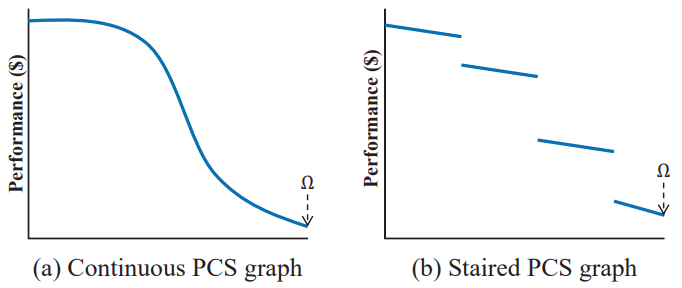
\includegraphics[width=0.8\linewidth]{Chapter-Introduction/Figures/stairs.png}
    \caption{Performance curves. (From ~\cite{oh2017finding})}
    \label{fig:chap1_stairs}
\end{figure}

To elaborate, if we sort the configurations from worst-performance to best and
plot configurations along the X-axis and performance along the
Y-axis. We expected a continuous graph
such as Figure~\ref{fig:chap1_stairs}(a), where high-valued (\$) is bad (worst performance is at the far left) and low-valued (\$) is good (best performance is at the
far right). Interestingly, Marker et al.~\cite{marker2014understanding} discovered that performance curves often occurs (in real world) as stairs, as in Figure 3b. Stairs arise from discrete feature decisions;
some features are highly-influential in performance while others
have little or no impact. Consequently, a few critical features
influences the performance while less important feature decisions alter the performance of nearby configurations only slightly (giving a stair its width and slope).

\noindent\textbf{Intuition}: From the literature, it is evident that most of the configuration options in a (given) software system does not affect the performance of the configurations. Hence, the central insight of this work is that random sampling with no regards to this specific feature of this problem is ineffective and hence adds additional cost. 

\noindent\textbf{Proposal}: This problem can be reformulated as a clustering problem, where we try to find an unsupervised method to cluster the configuration space into meaningful clusters. Once we have these clusters, we can use random samples (of configurations) from each of these clusters. This way, we can reduce redundant measurements.  

\section{Ranking}
Prior work in this area (including~\cite{nair2017faster}), tried to build accurate performance predictors, which can be used to predict the performance of a certain configuration. This work reflects on the prior work and asks: ``\textit{Our goal is to find a good configuration~\footnote{Good is defined as the distance from the optimal configuration} but, why does the prior work transform this problem into building an accurate model?}'' Another reason for this question is the very nature of the model building process previously described in Figure~\ref{fig:chap1_sampling_process}. We ask the question ``How does a user define \textit{Good}''? There is no way for the user to know whether a model can be build with MMRE less that 10\%. 

With respect to aforementioned questions, we drastically modify our approach to this problem. We hypothesize that to find the best performing configuration, we do not want a model which can return a predicted performance score which is as close to the actual performance score. Instead, we build a model which preserves the relative ordering of the configurations. 

\noindent\textbf{Intuition}: The central insight of this work is that exact performance
values (e.g., the response time of a software system) are not
required to rank configurations and to identify the optimal one. To elaborate more, let us assume that we have two humans (Adam---134cm, Billy---173cm) (analogous to configurations) and our objective is to identify the tallest person (Billy). To identify the tallest person, do we need a model which accurately predicts their height in a nano-meter scale? We can easily identify Billy even if the bad model predicted Adams height as 700cm and 890cm. 

\noindent\textbf{Proposal}: 
We show that, if we (slightly) relax the question
we ask, we can build useful predictors using very small sample sets.
Specifically, instead of asking ``How long will this configuration
run?'', we ask instead ``Will this configuration run faster than that
configuration?'' or ``Which is the fastest configuration?''.


\section{Sequential-Model Based Sampling}
Prior work in this area primarily used two strategies.
Firstly, researchers used machine learning to model the configuration
space. The model is built sequentially, where new
configurations are sampled randomly, and the quality or
accuracy of the model is measured using a holdout set. The
size of the holdout set in some cases could be up to 20\% of
the configuration space~\cite{nair2017using} and needs to be evaluated (i.e.,
measured) before even the model is fully built. This strategy
makes these methods not suitable in a practical setting since
the generated holdout set can be (very) expensive. Secondly,
the sequential model-based techniques used in prior work
relied on Gaussian Process Models (GPM) to reflect on the
configurations explored (or evaluated) so far~\cite{zuluaga2016varepsilon}. However,
GPMs do not scale well for software systems with more than
a dozen configuration options~\cite{wang2016bayesian}.



\noindent\textbf{Intuition}: 
To reduce the cost of sampling and eliminate the need for holdout set, we use sequential Model-based Optimization (SMBO). SMBO uses the Bayesian methodology to the iterative optimizer by incorporating a prior model (built using configuration which are already measured) on the space of possible target functions, $f$. By updating this model every time time a configuration is evaluated, a SMBO routine keeps a posterior model of the target function $f$. This posterior model is the surrogate $f^*$ for the function f (ground truth). Figure~\ref{fig:chap1_smbo} encapsulates the process.

\begin{figure}[!htbp]
    \centering
    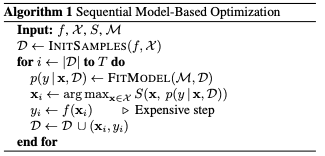
\includegraphics[width=0.6\linewidth]{Chapter-Introduction/Figures/bayesian_opt.png}
    \caption[Algorithm for SMBO methods]{Sequential Model-based Optimization. (From ~\url{http://tiny.cc/3hy80y})}
    \label{fig:chap1_smbo}
\end{figure}

\noindent\textbf{Proposal}:
We use the intuition present above to develop a method called FLASH.
The key idea of FLASH is to build a performance model
that is just accurate enough for differentiating better configurations
from the rest of the configuration space. Tolerating
the inaccuracy of the model is useful to reduce the cost
(measured in terms of the number of configurations evaluated)
and the time required to find the better configuration.
To increase the scalability of methods using GPM (Gaussian Process Models)---used widely in the machine learning domain, FLASH
replaces the GPMs with a fast and scalable decision tree learner.





\section{How to Read the Dissertation}
This dissertation is organized as self-contained chapters that together support
the thesis.

\textbf{Chapter~\ref{chapter:one}} explains, identifies and provides context for the research problem, articulates the objective, significance, and scope of the work.

\textbf{Chapter~\ref{chapter:background}} presents the background and related work in this area. The area of performance optimization has been explored not just in the domain of software engineering and has gained a lot of interest in the systems community as well. In general, there has been a considerable interest in the black-box optimization literature. In this chapter, an attempt has been made to describe the research work using the terminology used in the rest of the thesis.

\textbf{Chapter~\ref{chapter:WHAT}} describes the design and implementation
of \emph{WHAT}.
{\what}'s innovation is  
the use of the spectrum (eigenvalues) of the distance matrix
between the configurations of a configurable software system, to perform dimensionality reduction. Within that
reduced configuration space, many closely associated configurations can be studied
by executing only a few sample configurations. For the subject systems studied
here, a few dozen samples yield accurate and stable predictors---less than 10\,\% prediction error, with a standard deviation of less than 2\,\%.  
When compared to the state of the art, our approach (a)~requires 
2 to 10 times fewer samples to achieve similar prediction accuracies,
and (b)~its predictions are  more stable (i.e., have lower standard
deviation). 
Furthermore, we demonstrate that predictive models generated by
\what can be used by optimizers to discover system configurations that closely approach the optimal performance.


\textbf{Chapter~\ref{chapter:rank}} proposes using ranking models instead of regression models to save cost while finding good configurations. The central  insight of this chapter is that   
exact performance values (e.g., the response time of a software system) are not required to rank  configurations and to identify the optimal one. 
As shown by our experiments, performance models that are cheap to learn but inaccurate (with respect to the difference between actual and predicted performance) can still be used rank configurations and hence find the optimal configuration. This novel \emph{rank-based approach} allows us to significantly reduce the cost (in terms of number of measurements of sample configuration) as well as the time required to build performance models. We evaluate our approach with 21 scenarios based on 9 software systems and demonstrate that our approach is beneficial in 16 scenarios; for the remaining 5 scenarios, an accurate model can be built by using very few samples anyway, without the need for a rank-based approach.

In \textbf{Chapter~\ref{chapter:flash}}, we design and implement FLASH. The central insight of this paper is to use the prior knowledge (gained from prior runs) to choose the next promising configuration. This strategy reduces the effort (measured in terms of the number of measurements) required to find the (near) optimal configuration.  \flash can be used to solve single-objective (e.g., run-time) and can also be adapted to multi-objective (e.g., energy and runtime) performance optimization problems. 
We evaluate \flash  using 30 scenarios based on 7 software systems to demonstrate that \flash saves effort in 100\% and 80\% of cases in single-objective and multi-objective problems respectively by up to several orders of magnitude. 
% We also demonstrate how \flash is more scalable than other state of the art sequential model-based methods. 
% \textcolor{red}{TODO}
% Many design processes can be described as the exploration of options. Hence, 
% \flash can be applied to many areas.
% To demonstrate this,  we evaluate \flash, beside performance configuration optimization,  on standard search-based software engineering case studies   (release planning, process modeling, and sprint planning for agile development). 
% The superior performance
% of  \flash in these software systems, plus its better scalability and faster runtimes, makes us recommend this method XXX

In \textbf{Chapter~\ref{chapter:conclusion}}, we revisit the key contributions of this thesis and provide directions for future work.
\chapter{Background and Related Work}
\label{chapter:background}

This chapter describes the necessary background that is related to
the research problems addressed in this dissertation.
We first describe data-intensive computing and its storage architecture.
Next we discuss performance prediction for distributed systems.
Last, we discuss related work that uses the data-driven approach
to optimize system performance.



\chapter{Faster Discovery of Faster System Configurations with Spectral Learning}
\label{chapter:WHAT}
\noindent\textit{This chapter originally appeared as Nair, V., Menzies, T., Siegmund, N., \& Apel, S. (2017). Faster discovery of faster system configurations with spectral learning. Automated Software Engineering, 1-31. }





\section{Abstract}
Despite the huge spread and economical importance of configurable software systems, there is  unsatisfactory support in utilizing the full potential of these systems with respect to finding performance-optimal configurations.
Prior work on predicting the performance of software configurations suffered from either (a)~requiring far too many sample configurations or (b)~large variances in their predictions.
Both these problems can be avoided using the \what spectral learner.  
{\what}'s innovation is  
the use of the spectrum (eigenvalues) of the distance matrix
between the configurations of a configurable software system, to perform dimensionality reduction. Within that
reduced configuration space, many closely associated configurations can be studied
by executing only a few sample configurations. For the subject systems studied
here, a few dozen samples yield accurate and stable predictors---less than 10\,\% prediction error, with a standard deviation of less than 2\,\%.  
When compared to the state of the art, our approach (a)~requires 
2 to 10 times fewer samples to achieve similar prediction accuracies,
and (b)~its predictions are  more stable (i.e., have lower standard
deviation). 
%unclear: (i.e., much mean errors and standard deviations on the errors, refer to Figure 9-11)
Furthermore, we demonstrate that predictive models generated by
\what can be used by optimizers to discover system configurations that closely approach the optimal performance.
%\keywords{Performance Prediction \and Spectral Learning \and Decision Trees \and Search-Based Software Engineering \and Sampling.}

\section{Introduction}
 
%==Are these comments?== 
%Are feature/variability models too abstract for concrete reasoning?
%Or is it possible to use these models to predict specific properties 
%of programs generated from them? 

% Most software systems today are configurable. Despite the undeniable benefits
% of configurability, 
% large configuration spaces challenge developers, maintainers, and users. In the face of hundreds of configuration options, it is difficult to keep track of the effects of individual configuration options and their mutual interactions. So, predicting the performance of individual system configurations or determining the optimal configuration is often more guess work than engineering. In their recent paper, Xu et al.\ documented the  difficulties developers face
% with understanding  the configuration spaces of their systems~\cite{xu2015hey}. As a result, developers tend to ignore over $5/6$ths of the configuration options, which leaves considerable optimization potential untapped and induces major economic cost~\cite{xu2015hey}.

Addressing the challenge of performance prediction and optimization in the face of large configuration spaces, researchers have developed a number of approaches that rely on sampling and machine learning~\cite{siegmund2012predicting,guo2013variability,sarkar2015cost}.
While gaining some ground, state-of-the-art approaches face two problems: 
(a)~they require far too many sample configurations for learning or (b)~they are prone to large variances in their predictions. For example, prior work on predicting performance scores using regression-trees had to compile and execute hundreds to thousands of specific system configurations~\cite{guo2013variability}. 
% Other studies that tried to make far fewer execution samples resulted in predictors that were considerably inaccurate in their performance predictions.\todo[inline]{Which do you mean?}
A more balanced approach by Siegmund et al.\ is able to learn predictors for  configurable systems~\cite{siegmund2012predicting} with low mean errors, but with large variances of prediction accuracy  (e.g.\ in half of the results, the performance predictions for the Apache Web server were up to 50\,\% wrong). 
%My(Norbert) comment on this: you can't just take the worst heuristic here when the paper was about improving over this worst case...
 %\footnote{The predictions of \cite{siegmund2012predicting} had $\mu=19\%$ errors with $\sigma = 19.5\%$.}
  %that half they time, they could be up to 50\% incorrect\footnote{
 %The range  $\mu \pm 1.5*\sigma$  includes the
 %25th to 75th percentile range of a normal distribution   
%For the \cite{siegmund2012predicting} errors, that range is  0 to 49\%.}. 
% >> Where do you have this data from? Does not match with the paper.
% Vivek: You take the fault rate and standard deviation of the method which uses **almost** same  number of measurements. 
Guo et al.~\cite{guo2013variability} also proposed an incremental method to build a predictor model, which uses incremental random samples with steps equal to the number of configuration options (features) of the system. This approach also
suffered from  unstable predictions (e.g., predictions had a mean error of up to 22\,\%, with a standard deviation of up 46\,\%). Finally, Sarkar et al.~\cite{sarkar2015cost} proposed a proj\-ective-learning approach (using fewer measurements than Guo at al.\ and Siegmund et al.) to quickly compute  the number of sample configurations for learning a stable predictor. However, as we will discuss, after making that prediction, the total number of samples required for learning the predictor is comparatively high (up to hundreds of samples).

The problems of large sample sets and large variances in prediction can be avoided using the \what spectral learner, which is our main contribution.  
{\what}'s innovation is  the use of the spectrum (eigenvalues) of the distance matrix
between the configurations of a configurable system, to perform dimensionality reduction. Within that
reduced configuration space, many closely associated configurations can be studied
by measuring only a few samples.
In a number of experiments, we compared \what against the state-of-the-art approaches of Siegmund et al.~\cite{siegmund2012predicting}, Guo et al.~\cite{guo2013variability}, and Sarkar et al. \cite{sarkar2015cost} by means of six real-world configurable systems: Berkeley DB,  the Apache Web server, SQLite, the LLVM compiler, and the x264 video encoder.
We found that \what performs as well or better than prior approaches,
while  requiring far fewer samples (just a few dozen).
This is significant and most surprising, since some of the systems explored here have up to millions of possible configurations. 

Overall, we make the following contributions:
\begin{itemize}
\item We present a novel sampling and learning approach for predicting the performance of software configurations in the face of large configuration spaces. The approach is based on a
{\em spectral
learner} that uses an approximation to the first principal component of the configuration space to recursively cluster it, relying only on a few points as representatives of each cluster.
\item We demonstrate the practicality and generality of our approach by conducting experiments on six real-world configurable software systems (see Figure ~\ref{fig:systems}). The results show that our approach is more accurate (lower mean error) and more stable (lower standard deviation) than state-of-the-art approaches.
\item We report on a comparative analysis of our approach and three state-of-the-art approaches, demonstrating that our approach outperforms previous approaches in terms of sample size and prediction stability. A key finding is the utility of the principal component of a configuration space to  find informative samples from a large configuration space.
\end{itemize}
%More generally, this paper illustrates the value of spectral learning for software-engineering data sets. We recommend spectral learning for any analytics
%tasks with many options described by sets of attributes
%that might be noisy or redundant. For further details on why we make this recommendation, see Section~\ref{sect:sample}.

%The rest of the paper is organized as follows. Section 2 defines the terms used in the paper. Section 3 describes the background of the problem we are trying to tackle along with the data sets used in the experiments. Section 4 further explores the research question and finds association among them. Section 5 describes the experiment setup etc. Section 6 discusses the results and Section 7 the related work. This paper concludes after mentioning the threats to validity.
 
\section{Background \& Related Work}  
\label{sect:addit}

A configurable software system has a set $X$ of Boolean configuration options,\footnote{In this paper, we concentrate on Boolean options, as they make up the majority of all options; see Siegmund et al., for how to incorporate numeric options~\cite{SGA+15}.} also referred to as features or independent variables in our setting.
We denote the number of features of system $S$ as $n$. The configuration space of $S$ can be represented by a Boolean space ${Z}_{2}^{n}$, which is denoted by $F$. All valid configurations of $S$ belong to a set $V$, 
which is represented by vectors $\vec{C_i}$ (with $1\leq i\leq \left\vert{V}\right\vert$) in ${Z}_{2}^{n}$. Each element of a configuration represents a feature, which can either be \emph{True} or \emph{False}, based on whether the feature is selected or not. 
% We denote the number of features in the system as $n$. All the features of a system can be represents a boolean/binary space (${Z}_{2}^{n}$)--- $F$, where $n$ is the number of features of the system. Every software system has a set of valid configurations ($V$) which is represented as a vector $\vec{C} \in {Z}_{2}^{n}$, where ${Z}_{2}^{n}$
% % http://math.stackexchange.com/questions/892094/notation-for-show-that-a-variable-is-binary
% is Boolean $n$-space i.e. each feature of a configurations is assigned $\mathit{True}$ and $\mathit{False}$ otherwise, based on whether the feature was selected or not.  
Each valid instance of a vector (i.e., a configuration) has a corresponding performance score associated to it. 

The literature offers two approaches to performance prediction of software configurations: a {\em maximal sampling} and a {\em minimal sampling} approach: 
With {\em maximal sampling}, we compile all  possible configurations and record the associated performance scores. 
Maximal sampling  can be impractically slow. For example, the performance data used in this paper required  26 days of CPU time for measuring (and much longer, if we also count the time required for compiling the code prior to execution). 
 Other researchers have commented that,  in 
 real world scenarios, the cost of acquiring the optimal configuration is overly expensive and time consuming \cite{weiss2008maximizing}.
 
 If collecting performance scores of all configurations is impractical,  {\em minimal sampling} 
 can be used to intelligently select and execute just enough configurations (i.e., samples) to build a
 predictive model.
 For example, Zhang et al.~\cite{zhang2015performance} approximate the
configuration space as a Fourier series, after which they can derive an expression showing how many configurations must be studied
 to build predictive models with a given error. While a theoretically satisfying result, that approach still needs thousands to hundreds of thousands of executions of sample
 configurations.  

Another set of approaches are the four "additive" {\em minimal sampling} methods of Siegmund et al.~\cite{siegmund2012predicting}.
Their first method, called feature-wise sampling ({\em FW}), is their basic method.
To explain {\em FW}, we note that, from a configurable software system, it is theoretically possible to enumerate many or all of the valid configurations\footnote{Though, in practice, this can be very difficult. For example, in models like the Linux Kernel such an enumeration is practically impossible ~\cite{sayyad13b}.}. 
Since each configuration ($\vec{C_i}$) is a vector of $n$ Booleans, it  is possible to use this information to isolate examples of how much each feature individually contributes to the total run time:
\begin{enumerate}
\item Find a pair of  configurations $\vec{C_i}$ and $\vec{C}_2$, where $\vec{C}_2$ uses exactly the same features as $\vec{C_i}$, plus one  extra feature $f_i$.
\item Set the run time $\Pi(f_i)$ for feature $f_i$ to be the difference in the performance scores between $\vec{C_2}$ and $\vec{C_i}$.
\item The run time  for a new configuration  $\vec{C}_i$ (with $1\leq i\leq \left\vert{V}\right\vert$) that has not been sampled before is then the sum of the run time of its features, as determined before:
\begin{equation}
  \Pi(C_i) = \sum_{f_j \in C_i}\Pi(f_j)  
\end{equation}
\end{enumerate}

When many pairs, such as ${\vec{C_1},\vec{C}_2}$, satisfy the criteria of point~1, Siegmund et al.\ used the 
pair that covers the {\em smallest} number of features. Their minimal sampling method, {\em FW},
compiles and executes only these smallest $C_1$ and $C_2$ configurations. 
Siegmund et al.\ also offers three extensions to the basic method, which are based on sampling
not just the smallest $\vec{C_i}$,$\vec{C_2}$  pairs, but also any configurations with {\em interactions} between features. 
All the following minimal sampling policies compile and   execute valid configurations selected via one of three heuristics:

\begin{description}
\item[{\em PW (pair-wise):}] For each pair of features, try to find a configuration that contains the pair and has a minimal number of features selected. 
\item[{\em HO (higher-order):}] Select extra configurations, in which three features, $f_1,f_2,f_3$, are selected if two of the following pair-wise interactions exist: $(f_1,f_2)$ and $(f_2,f_3)$ and $(f_1,f_3)$.
\item[{\em HS (hot-spot):}] Select extra configurations that contain features that are
frequently interacting with other features. 
\end{description}


Guo et al.~\cite{guo2013variability} proposed a progressive random sampling approach, which samples in steps of the number of features of the software system in question. They used the sampled configurations to train a regression tree, which is then used to predict the performance scores of other system configurations. The termination criterion of this approach is based on a heuristic, similar to the {\em PW} heuristics of Siegmund et al. 

Sarkar et al.~\cite{sarkar2015cost} proposed a cost model for predicting the effort (or cost) required to generate an accurate predictive model. The user can use this model to decide whether to go ahead and build the predictive model. This method randomly samples configurations and uses a heuristic based on feature frequencies as termination criterion. The samples are then used to train a regression tree; the accuracy of the model is measured by using a test set (where the size of the training set is equal to size of the test set). One of four projective functions (e.g., exponential) is selected based on how correlated they are to  accuracy measures. The projective function is used to approximate the accuracy-measure curve, and the elbow point of the curve is then used as the optimal sample size. Once the optimal size is known, Sarkar et al.\ uses the approach of Guo et al.\ to build the actual prediction model.  


The advantage of these previous approaches is that, unlike  the results of Zhang et al., they require only dozens to hundreds of samples. Also, like our approach, they do not require to enumerate all configurations, which is important for highly configurable software systems. 
That said, as shown by our experiments (see Section~\ref{sec:experiments}), these approaches produce estimates with  larger mean errors and partially larger variances than our approach. While sometimes the approach by Sarkar et al. results in  models with (slightly)
lower mean error rates, it still requires a considerably larger number of samples (up to hundreds, while \what requires only few dozen).
 
 \section{Approach}

\subsection{Spectral Learning}\label{sect:spect}

The minimal sampling method proposed in this paper is based on a spectral-learning algorithm
that  explores the spectrum (eigenvalues) of the distance matrix between  configurations.
In theory, such spectral learners are an appropriate method to handle noisy, redundant, and tightly inter-connected variables, for the following reasons:
When data sets have many irrelevancies or closely associated data parameters $d$, then
only a few eigenvectors $e$, $e \ll d$  are required to characterize the data.
In that reduced space:
\begin{itemize}
\item
Multiple inter-connected variables $i,j,k \subseteq d$ can be represented
by a single eigenvector;
\item
Noisy variables from $d$ are
ignored, because they  do not contribute to the signal in the data;
\item
Variables  become (approximately) parallel lines
in $e$ space. For  redundancies \mbox{$i,j \in d$}, we
can ignore $j$
since effects that change over $j$ also
change in the same way over $i$;
\end{itemize}
That is, in theory, samples of configurations drawn via an eigenspace sampling method
would not get confused by noisy, redundant, or tightly inter-connected variables. Accordingly,
we expect predictions built from that sample to have  lower mean errors and lower variances on that error.

Spectral methods have been used before for a variety of data mining applications~\cite{kamvar2003spectral}.
Algorithms, such as PDDP~\cite{boley98}, use spectral methods, such as principle component analysis (PCA), to
recursively divide data into smaller regions.  Software-analytics researchers use spectral methods (again, PCA) as a pre-processor prior to data mining  to reduce noise in software-related data sets~\cite{theisen2015approximating}.
However, to the best of our knowledge, spectral methods have not been used before in software engineering as a basis of a minimal sampling method.


\what is somewhat different from other spectral
learners explored in, for instance, image processing applications~\cite{shi00}.
Work on image processing does not address
defining a minimal sampling policy to predict performance scores.
Also, a standard spectral method requires an $O(N^2)$ matrix multiplication to compute the components
of PCA~\cite{ilin10}. Worse, in the case of hierarchical division methods, such as PDDP,
the polynomial-time inference must be repeated at every level of the hierarchy.
Competitive results can be achieved
using an $O(2N)$ analysis that we have developed previously~\cite{me12d}, which is  based on  a heuristic proposed by Faloutsos and Lin~\cite{Faloutsos1995} (which Platt has shown computes a Nystr\"om approximation to the first component of PCA~\cite{platt05}).

% \todo[inline]{This paragraph requires a bit more clarification and a relation to the notation introduced in section 2. What is n? What are examples?}  
Our approach inputs $N$ (with $1\leq \left\vert{N}\right\vert\leq \left\vert{V}\right\vert$)
valid configurations ($\vec{C}$), $N_1,N_2,...$, and then:
\begin{enumerate}
\item
Picks any
point $N_i$ ($1\leq i \leq\left\vert{N}\right\vert$) at random;
\item
Finds
 the point  {\em West}~$\in N$ that is
furthest away from $N_i$;
\item Finds the point {\em East}~$\in N$
that is furthest from {\em West}.
\end{enumerate}
The line joining {\em East}
and {\em West} is our approximation for the first principal component.
Using the distance calculation shown in Equation~\ref{eq:dist}, 
we define $\delta$ to be the distance between {\em East}
and {\em West}. 
% \todo[inline]{What is $c$? Changed to $\delta$}
\what uses this distance ($\delta$) to divide all the configurations as follows:
The value $x_i$ is the projection of $N_i$
on the line  running  from {\em East} to {\em West}\footnote{The projection of $N_i$ can be calculated in the following way:\newline $a = \mathit{dist}(\mathit{East}, N_i); b = \mathit{dist}(\mathit{West}, N_i);  x_i = \sqrt{\frac{a^2 - b^2 + \delta^2}{2\delta}}$.
}.  We divide
the examples based on the median value of the projection of $x_i$. Now, we have two clusters of data divided based on the projection values (of $N_i$) on the line joining {\em East} and {\em West}. This process is applied recursively on these clusters until a predefined stopping condition. In our study, the  recursive splitting of the $N_i$'s stops when a sub-region
contains less than  $\sqrt{|N|}$ examples.
\begin{equation}
    \mathit{dist}(x, y) =     
    \begin{cases}
      \sqrt{\sum_i(x_i-y_i)^2}
      & \text{if $x_i$ and $y_i$ is numeric}\\
        \begin{cases}
            0, & \text{ if $x_i = y_i$}\\
            1, & \text{ otherwise}\\
        \end{cases}
        & \text{if $x_i$ and $y_i$ is Boolean}\\
    \end{cases}
    \label{eq:dist}
\end{equation}
We explore this approach for three reasons:
\begin{itemize}
\item
{\em It is very fast}:
This process requires only $2|n|$ distance comparisons
per level of recursion, which is far less than the $O(N^2)$
required by PCA~\cite{Du2008}
or other  algorithms such as K-Means~\cite{hamerly2010making}.
\item
{\em It is not domain-specific}:
Unlike traditional PCA, our approach is general in that it does not assume that all the variables are numeric. As shown in Equation~\ref{eq:dist},\footnote{In our study, $\mathit{dist}$ accepts configurations ($\vec{C}$) and returns the distance between them. If $x_i$ and $y_i$ $\in {R}^n$, then the distance function would be same as the standard Euclidean distance.} we can approximate distances for both numeric and non-numeric data (e.g., Boolean).

\item
{\em It reduces the dimensionality problem}:
This technique explores the underlying dimension (first principal component) without getting confused by noisy, related, and highly associated variables.
\end{itemize}

\subsection{Spectral Sampling}\label{sect:sample}
When the above clustering method terminates, our  sampling policy (which we will call $S_1$:Random) is then applied:
\begin{description}
\item[{\em Random sampling ($S_1$):}] compile and execute one  configuration,  picked at random, from each leaf cluster;
\end{description}
We use this sampling policy, because (as we will show later) it performs better than:
\begin{description}
\item[{\em East-West sampling ($S_2$):}] compile and execute the {\em East} and {\em West} poles of the leaf clusters;
\item[{\em Exemplar sampling ($S_3$):}] compile and execute all items in all leaves and return the one
with lowest performance score.
\end{description}

Note that $S_3$ is {\em not} a {\em minimal} sampling policy (since it executes all configurations). 
We use it here as one  baseline
against which we can compare the other, more minimal, sampling policies. In the results
that follow, we also compare our 
sampling methods against another baseline using information gathered after executing
all configurations.

\subsection{Regression-Tree Learning} \label{rtlearning}
After collecting the data using one of the sampling policies ($S_1$, $S_2$, or $S_3$), as described in Section \ref{sect:sample}, we  use a CART regression-tree learner~\cite{breiman1984} to build a performance predictor. Regression-tree learners seek the attribute-range split that most increases
our ability to make accurate predictions.
CART explores splits that divide $N$ samples  into two sets  $A$ and $B$, where each set  has a  standard deviation on the target variable of $\sigma_1$ and  $\sigma_2$.
CART finds the ``best'' split defined as the split that minimizes $\frac{A}{N}\sigma_1 + \frac{B}{N}\sigma_2$.
Using this best split, CART divides the data recursively.

In summary, \what  combines:
\begin{itemize}
\item
The FASTMAP method of Faloutsos and Lin~\cite{Faloutsos1995};

\item A spectral-learning algorithm initially   inspired by    Boley's PDDP system~\cite{boley98}, which we modify
by replacing  PCA with FASTMAP (called
``WHERE'' in prior work ~\cite{me12d});

\item
The sampling policy that explores the leaf clusters found by this recursive division;

\item 
The CART regression-tree learner that converts the data from the samples collected by sampling policy 
into a run-time prediction model~\cite{breiman1984}.
\end{itemize}
That is,
\begin{center}
\begin{tabular}{rcl}
WHERE& = &PDDP $-$ PCA $+$ FASTMAP\\[1.5ex] 
\what& =  & WHERE $+$ SamplingPolicy $+$ CART
\end{tabular}
\end{center}
This unique combination of methods has not been previously explored in the
software-engineering literature.
% \todo[inline]{PLEASE REMOVE-In the remaining text we dont need to mention S1:Random, as it is part of \what, be the above definition. Since we compare different sampling techniques in first research question, I think it is necessary to mention the sampling policy along with \what}

\section{Experiments}
\label{sec:experiments}
All materials required for reproducing this work are available at \url{https://goo.gl/689Dve}.


\subsection{Research Questions} 

We formulate our research questions in terms of the challenges of
exploring large complex configuration spaces.
Since our model explores the spectral space, our hypothesis is that only a small
number of samples is required to explore the whole space.
However, a prediction model built from a very small sample of the configuration space might
be very inaccurate and unstable, that is, it may exhibit very large mean prediction errors and variances on the prediction error.

%Could be removed if space is needed
Also, if we learn models from small regions of the training data,
it is  possible that a learner will miss {\em trends} in the data
between the sample points. Such trends are useful when building {\em optimizers}
(i.e., systems that input one configuration and propose an alternate
configuration that has, for instance,  a better performance). Such optimizers might
need to evaluate hundreds to millions of alternate configurations. 
To speed up that process, optimizers can use a {\em surrogate model}\,\footnote{Also known as response surface methods, meta models, or emulators.}
that  mimics the outputs of a system of interest, while being computationally cheap(er) to evaluate~\cite{loshchilov13}. For example, when optimizing
performance scores, we might ask a CART  for a performance
prediction (rather than compile and execute
the corresponding configuration).  Note that such surrogate-based
reasoning critically depends on how well the surrogate can guide optimization.


Therefore, to assess feasibility of our sampling policies, we must consider:
\begin{itemize}
\item Performance scores generated from our minimal sampling policy;
\item The variance of the error rates when comparing predicted performance scores with actual ones;
%the next point should always be true. otherwise, what would be the reason to do that?!
\item The optimization support offered by the performance predictor (i.e., can the model work in tandem with other off-the-shelf optimizers to generate useful solutions).
\end{itemize}

%\vfill\eject
The above considerations lead to four research questions:
\begin{description}
\item[{\em RQ1:}] {\em Can  \what generate good predictions after
executing only a small number of configurations?}
\end{description}
Here, by ``good'' we mean that the predictions made by models that were trained using sampling with \what are as accurate, or more accurate,
as those generated from models supplied with more samples.
\begin{description}
\item[{\em RQ2:}] {\em
Does less data used in building the models cause larger variances in the predicted values?}
\item[{\em RQ3:}] {\em
Can ``good'' surrogate models (to be used in optimizers)
be built from minimal samples?}
\end{description}
Note that {\bf RQ2} and {\bf RQ3} are of particular concern with our approach,
since our goal is to sample as little as possible from the configuration space.
\begin{description}
\item[{\em RQ4:}] {\em How good is \what compared to the state of the art of
learning performance predictors from configurable software systems?}
\end{description}

To answer RQ4, we will compare \what 
          against approaches presented by Siegmund et al.~\cite{siegmund2012predicting}, Guo et al.~\cite{guo2013variability}, and Sarkar et al.~\cite{sarkar2015cost}.
 

\begin{figure}[tbh]\small
\framebox[\columnwidth][c]{
\begin{tabular}{lrrr}
\multicolumn{4}{p{.95\linewidth}}{
\textbf{Berkeley DB C Edition (BDBC)} is an embedded database system written in C. It is one of the most deployed databases in the world, due to its low binary footprint and its configuration abilities. We used the benchmark provided by the vendor to measure response time.}\\
%
\multicolumn{4}{p{.95\linewidth}}{
\textbf{Berkeley DB Java Edition (BDBJ)} is a complete re-development in Java with full SQL support. Again, we used a benchmark provided by the vendor measuring response time.}\\
%
\multicolumn{4}{p{.95\linewidth}}{
\textbf{Apache} is a prominent open-source Web server that comes with various configuration options. To measure performance, we used the tools autobench and httperf to generate load on the Web server. We increased the load until the server could not handle any further requests and marked the maximum load as the performance value.}\\
%
\multicolumn{4}{p{.95\linewidth}}{
\textbf{SQLite} is an embedded database system deployed over several millions of devices. It supports a vast number of configuration options in terms of compiler flags. As benchmark, we used the benchmark provided by the vendor and measured the response time.}\\
%
\multicolumn{4}{p{.95\linewidth}}{
\textbf{LLVM} is a compiler infrastructure written in C++. It provides various configuration options to tailor the compilation process. As benchmark, we measured the time to compile LLVM's test suite.}\\
%
\multicolumn{4}{p{.95\linewidth}}{
\textbf{x264} is a video encoder in C that provides configuration options to adjust output quality of encoded video files. As benchmark, we encoded the Sintel trailer (735\,MB) from AVI to the xH.264 codec and measured encoding time.}\\[4ex]
\hline
System & LOC & Features & Configurations\\\hline
BDBC   & 219,811 & 18 & 2,560\\
BDBJ   & 42,596 & 32  & 400\\
Apache & 230,277 & 9 & 192\\
SQLite & 312,625 & 39 & 3,932,160\\
LLVM & 47,549 & 11 & 1,024\\
x264 & 45,743 & 16 & 1,152\\\hline
\end{tabular}
}
\caption[Subject systems to test \what]{Subject systems used in the experiments.}\label{fig:systems}
\end{figure}



\subsection{Subject Systems}
\label{sec:subject_systems}
The configurable systems we used in our experiments are described in Figure \ref{fig:systems}.
Note, with ``predicting performance'', we 
mean predicting performance scores of the subject systems while executing test suites provided by the developers or the community, as described in Figure~\ref{fig:systems}.
To compare the predictions of our and prior approaches with actual performance measures, we use data sets that have been obtained by
measuring {\em nearly all} configurations\footnote{http://openscience.us/repo/performance-predict/cpm.html}.
We say {\em nearly all} configurations, for the following reasoning: For 
all except one of our subject systems, the total number of valid configurations
was tractable (192 to 2560). However,  SQLite has 3,932,160 
possible configurations, which is an impractically large number of configurations to test whether our predictions are accurate and stable. Hence, for SQLite, we use the 4500 samples for testing prediction accuracy and stability, which we could collect in one day of CPU time. Taking this into account, we will pay particular attention to the variance of the SQLite results.




\subsection{Experimental Rig}


{\bf RQ1} and {\bf RQ2} require the construction and assessment of numerous runtime predictors from small samples
of the data. The following rig implements that construction process.

For each configurable software system, we built a table of data, one row per valid configuration. We then ran all configurations of all software systems
and recorded the performance scores (i.e., that are invoked by a benchmark).
The exception is SQLite for which we measured only the
configurations needed to detect interactions and additionally
100 random configurations to evaluate the accuracy of
predictions.  
% \todo[inline]{In Subject Systems we say that we use 4500 samples. In general, this discussion is redundant; I would remove it from Subject Systems.}
To this table, we added a column showing the performance score obtained from the actual measurements for each configuration.

Note that the following procedure ensures that
we \textbf{never} test any prediction model on the data used to learn that model. Next, we repeated the following procedure 20 times (the figure of 20 repetitions was
selected using the Central Limit Theorem): 
For each system in \{BDBC, BDBJ, Apache, SQLite, LLVM, x264\}
\begin{itemize}
\item Randomize the order of the rows in their table of data;
\item For $X$ in \{10, 20, 30, ... , 90\};
\begin{itemize}
\item Let {\em Train} be the first $X$\,\% of the data 
\item Let {\em Test} be the rest of the data;
\item Pass {\em Train} to \what to select   sample   configurations;
\item Determine the performance scores associated with these configurations. This corresponds to a table lookup, but would entail compiling and executing a system configuration in a practical setting.
\item Using the {\em Train}  data and their performance scores, build a performance predictor using CART.
\item Using the {\em Test} data, assess the accuracy of the predictor using the error 
measure of \eq{err} (see below).
\end{itemize}
\end{itemize}


% \todo[inline]{Check the correct placement of this paragraph}
The validity of the predictors built by the regression tree is verified on testing data. 
For each  test item, we determine how long it {\em actually} takes to run the corresponding system configuration and compare the actual measured performance to the {\em prediction} from CART. The resulting prediction error is then computed using:
\begin{equation}\label{eq:err}
\mathit{error}=\frac{\mid\mathit{predicted} - \mathit{actual}\mid}{\mathit{actual}}*100
\end{equation}
(Aside: It is reasonable to ask why this metrics and not some of the others proposed
in the literature (e.g sum absolute residuals). In short, our results are stable
across a range of different metrics. For example, the results of this paper have
been repeated using sum of absolute residuals and, in those other results,
we seen the same ranking of methods; see  http://tiny.cc/sumAR.)

{\bf RQ2} requires testing the standard deviation of the prediction error rate. To support that test, we:
\begin{itemize}
\item Determine the $X$-th point in the above experiments, where all predictions stop improving (elbow point);
\item Measure the standard deviation of the error at this point, across our 20 repeats.
\end{itemize}
As shown in Figure~\ref{fig:sampling_accuracy}, all our results plateaued after studying $X=40$\,\% of the valid configurations\footnote{Just to clarify one frequently asked question about this work, we note
that our rig ``studies'' 40\,\% of the data. We do not mean that our predictive models
 require accessing the performance scores from the 40\,\% of the data. Rather, by ``study'' we mean   reflect 
 on a sample of configurations to determine what minimal subset of that
sample deserves to be compiled and executed.}.
 Hence to answer {\bf RQ2}, we will compare all 20 predictions at $X=40$\,\%.
 
{\bf RQ3}   uses the learned regression tree as a {\em surrogate model} within an optimizer; 
\bi
\item Take   $X=40\,\%$ of the configurations;
\item Apply \what to build a CART model using some minimal sample taken from that 40\,\%;
\item Use that CART model within some standard optimizer while searching for 
configurations with least runtime;
\item  Compare the faster configurations found in this manner with the fastest configuration
known for that system.
\ei
This last item requires access to a ground truth of performance scores for a  
large number of configurations. For this experiment, we have access to that ground truth
(since we have access to all system configurations, except for SQLite). Note that such a ground truth
would not be needed when practitioners choose to use \what in their own work (it is only for our empirical investigation).


For the sake of completeness, we explored
a range of optimizers seen in the   literature in this second experiment:  DE~\cite{storn1997differential}, NSGA-II~\cite{deb00afast},
and our own GALE~\cite{krall2014gale,zuluaga2013active} system.   Normally,
it would be  reasonable to ask
why we used those three, and not the hundreds of other 
optimizers described in the literature~\cite{fletcher13,harman12}. However,
as shown below, all these optimizers in this
domain exhibited  very similar
behavior (all found configurations close to the
best case performance). Hence, the specific
choice of optimizer is not a critical
variable in  our analysis.


\begin{figure}[t]
\centering
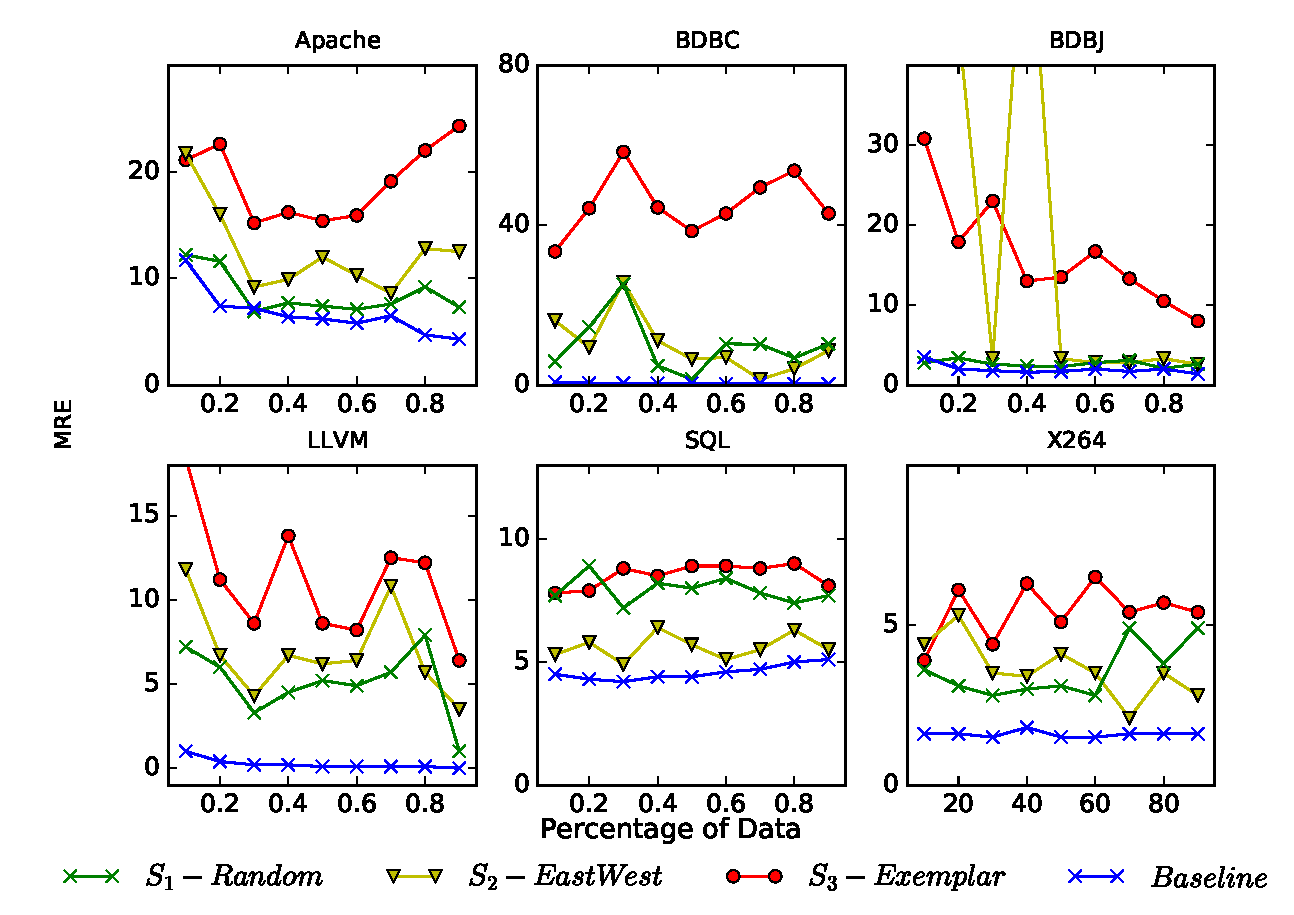
\includegraphics[width=\columnwidth]{Figures/SamplingAccuracy}
\caption[Errors of the predictions made by \what.]{Errors of the predictions made by \what with four different
sampling policies. Note that, on the y-axis,  {\em lower} errors are {\em better}.
}
\label{fig:sampling_accuracy}
\end{figure}

\section{Results}
\subsection{RQ1}

\begin{center}
{\em Can  \what generate good predictions after
executing only a small number of configurations?}
\end{center}

\noindent Figure~\ref{fig:sampling_accuracy} shows the mean errors of the predictors learned
after taking $X$\,\% of the configurations, then asking  \what and some sampling method ($S_1$, $S_2$, and $S_3$)
to (a)~find what configurations to measure; then (b)~asking CART to build a predictor
using these measurements. The horizontal axis of the plots shows what $X$\,\%
of the configurations are studied; the vertical axis shows the mean relative error (from \eq{err}).
In that figure:
\begin{itemize}
\item
The $\times$\hspace{-2pt}---\hspace{-2pt}$\times$ lines in Figure~\ref{fig:sampling_accuracy} show a {\em baseline} result
where data from the performance scores of 100\,\% of  configurations were used by CART
to build a runtime predictor.
\item
The other lines show the results using the sampling methods defined in Section~\ref{sect:sample}.
Note that these sampling methods used  runtime data only from a
subset of 100\,\% of the performance scores seen in configurations
from 0 to X\,\%.
\end{itemize}

% \todo[inline]{PLEASE REMOVE - Actually, RQ1 does not say anything about varying the sampling policy; Furthermore, we have defined: \what =  WHERE $+$ $S_1$:Random $+$ CART, so \what plus S2... makes no sense. Vivek: I have changed the definition of WHAT to sampling policy because we are making a claim that any random point is better. Our recent studies have shown that using using outlier is not a good representative of a cluster}

In \fig{sampling_accuracy}, {\em lower} y-axis values  are {\em better} since this means lower
prediction errors. Overall, we find that:
\begin{itemize}

\item Some software systems exhibit large variances in their error rate, below $X=40$\,\% (e.g., BDBC and BDBJ).
\item Above $X=40$\,\%, there is little effect on the overall change of the sampling methods.
\item
Mostly, $S_3$ shows the highest overall error, 
so that it cannot be recommended.
\item Always, the   $\times$\hspace{-2pt}---\hspace{-2pt}$\times$ baseline shows the lowest errors, which is to be
expected since predictors built on the baseline have access to all data.
\item
We see a trend that the error of  $S_1$ and $S_2$ are within $5$\,\% of the {\em baseline} results.
Hence, we can recommend these two minimal sampling methods.
\end{itemize}

\begin{figure}[t]
\centering
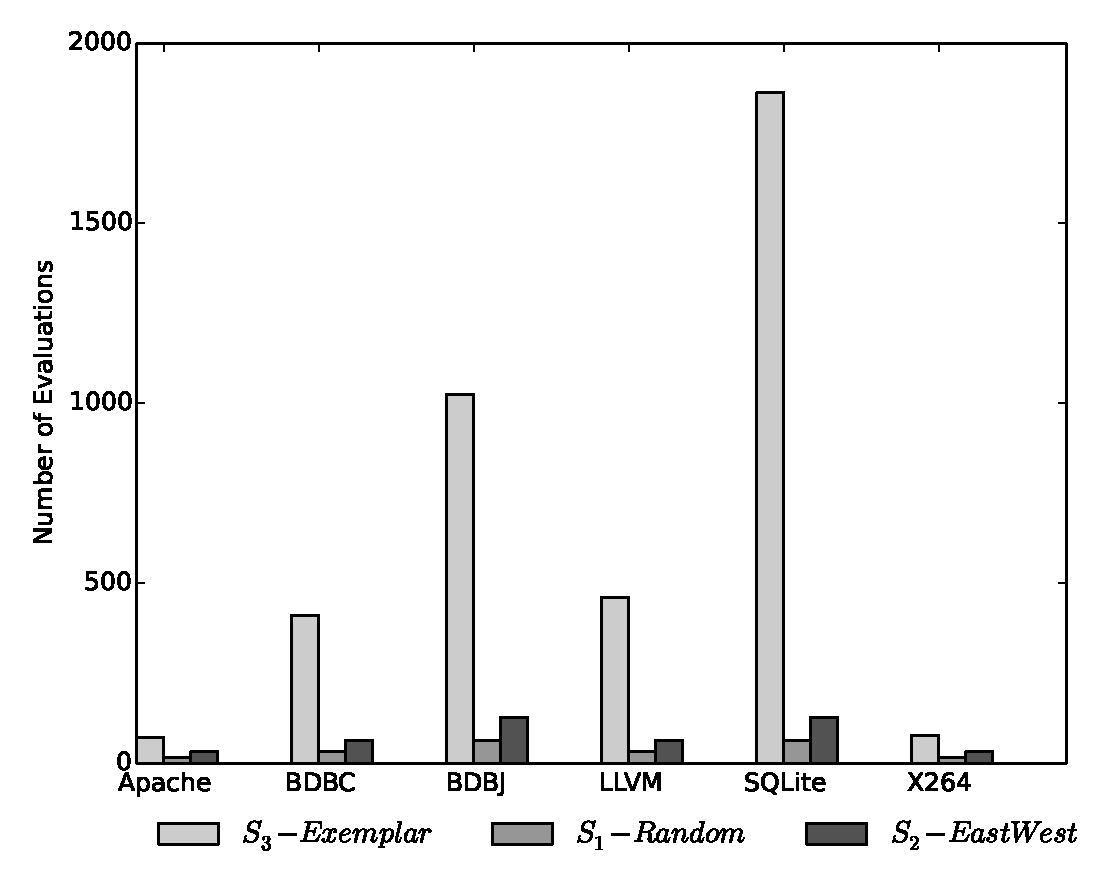
\includegraphics[width=0.75\columnwidth]{Figures/evaluation_graph}
\caption[Comparing evaluations of different sampling policies of \what.]{Comparing evaluations of different sampling policies. We see that the number of configurations evaluated for $S_2$ is twice as high as $S_1$, as it selects 2 points from each cluster, where as  $S_1$ selects only 1 point. }\label{fig:Evaluations}
\end{figure}

\fig{Evaluations} provides information about which  of    $S_1$ or $S_2$ we should recommend.
This figure displays data taken from the $X=40$\,\% point of \fig{sampling_accuracy} and displays
how many performance scores of configurations are needed by our sub-sampling methods (while
reflecting on the configurations seen in the range $0\le X \le 40$). Note that:
\begin{itemize}
\item
$S_3$ needs up to thousands of performance-score points, 
so it cannot be recommended as minimal-sampling policy;
\item $S_2$ needs twice as much performance-score information as 
$S_1$ ($S_2$ uses {\em two} samples per leaf cluster  while
$S_1$ uses only {\em one}).
\item $S_1$ needs performance-score information on only a few dozen (or less) configurations to generate
the predictions with the lower errors seen in \fig{sampling_accuracy}.
\end{itemize}

Combining the results of \fig{sampling_accuracy} and \fig{Evaluations}, we conclude that:

\begin{myshadowbox}
$S_1$ is our preferred spectral sampling method. Furthermore,
the answer to {\bf RQ1} is ``yes'', because applying \what{}, we can (a)~generate runtime predictors
using just a few dozens of sample performance scores; 
and (b)~these predictions have error rates
within 5\,\% of the error rates seen if predictors are built from information about all performance scores.
\end{myshadowbox}




\subsection{RQ2}

\begin{center}
{\em
Do less data used in building models cause larger variances in the predicted values?}
\end{center}


Two competing effects can cause increased or decreased  variances in 
runtime predictions.
The   less we sample the configuration space,
the less we constrain model generation in that space. Hence, one effect that can be expected
is that models learned
from too few samples exhibit large variances. 
But,
a  compensating effect can be introduced by sampling from the spectral space
since that space contains fewer confusing or correlated variables than the raw configuration space.
\fig{Variance} reports which one of these two competing effects are dominant. 
\fig{sampling_accuracy} shows that after some initial fluctuations,
after seeing $X=40$\,\% of the configurations, the variances in prediction errors reduces to nearly zero.


\begin{figure}[tbh]
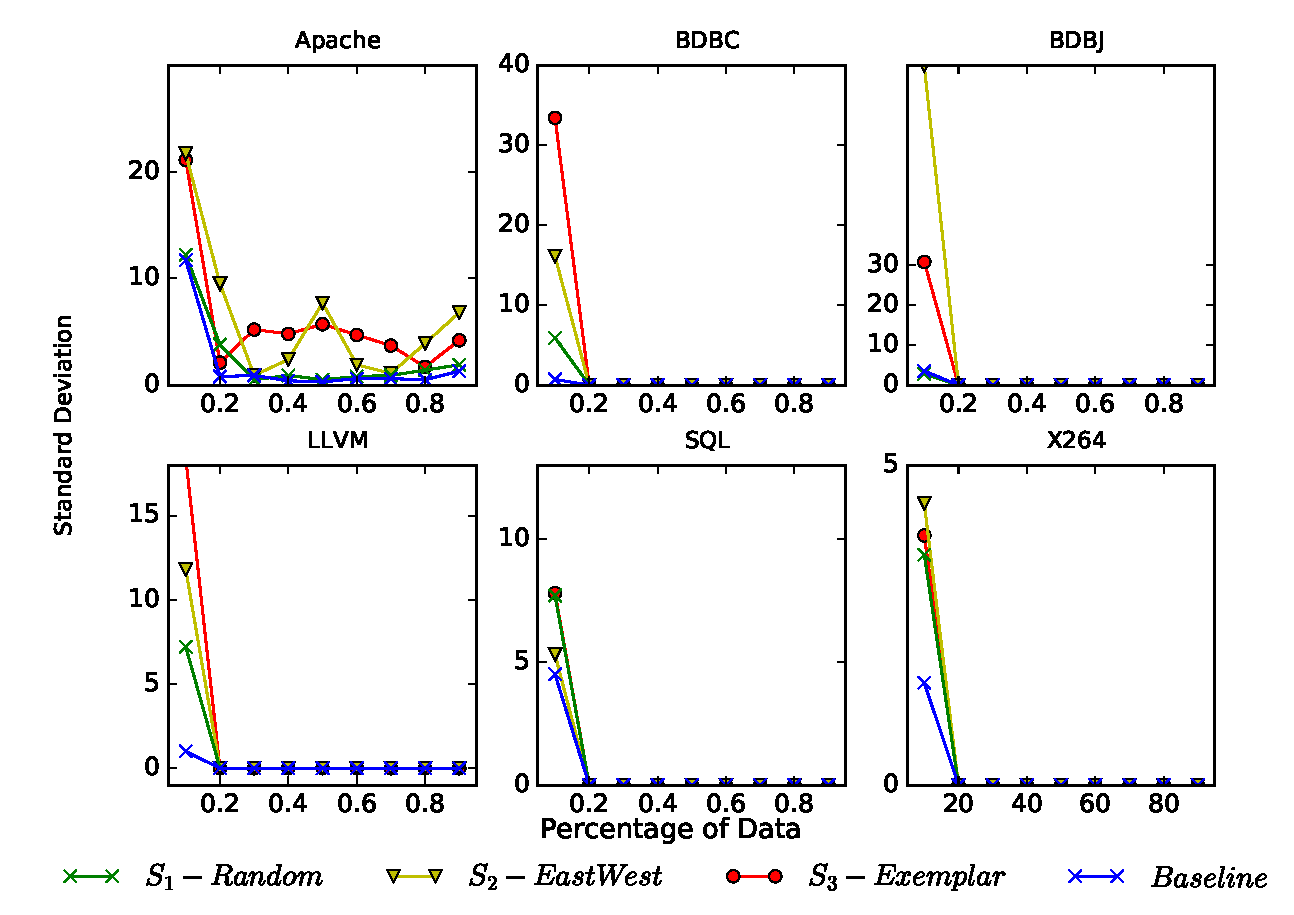
\includegraphics[width=\columnwidth]{Figures/Variance}
\centering
\caption[Standard deviations of different sampling strategies of \what]{Standard deviations seen at various points of  \fig{sampling_accuracy}.}\label{fig:Variance}
\end{figure}

\begin{myshadowbox}
Hence, we answer {\bf RQ2} with ``no'': Selecting a small number of samples does not necessarily increase variance (at least to say, not in this domain).
\end{myshadowbox}


\subsection{RQ3}

\begin{center}
{\em
Can ``good'' surrogate models (to be used in optimizers)
be built from minimal samples?}
\end{center}

The results of answering {\bf RQ1} and {\bf RQ2} suggest to use \what (with $S_1$) to build runtime predictors from a small sample of  data. {\bf RQ3}
asks if that predictor can be used by an optimizer to infer what {\em other} configurations correspond to system configurations with fast performance scores.
To answer this question,  we ran  a random set of 100 
configurations, 20 times, and related that baseline to three optimizers (GALE~\cite{krall2014gale}, DE~\cite{storn1997differential} and  NSGA-II~\cite{deb00afast}) using their
default parameters.
 
When these three optimizers mutated existing configurations to suggest new ones,
these mutations were checked for validity. Any mutants that violated the system's constraints (e.g., a feature excluding another feature) were rejected
and the survivors were ``evaluated'' by asking the CART surrogate model.
%(the  CART regression-tree learned from \what+$S_1$:Random, built using the methods of {\bf RQ1}).
These evaluations either rejected the mutant or used it in generation $i+1$, as the basis for a search for more, possibly
better  mutants.




\fig{performance_graph} shows the configurations found by three optimizers projected onto the ground truth of the performance scores of nearly
all configurations (see Section~\ref{sec:subject_systems}). Again note that, while we use that ground truth for the validation of these results, our optimizers 
used only a small part of that ground-truth data in their search for the fastest configurations (see the \what + $S_1$
results of \fig{Evaluations}).


\begin{figure}[tb]
\centering
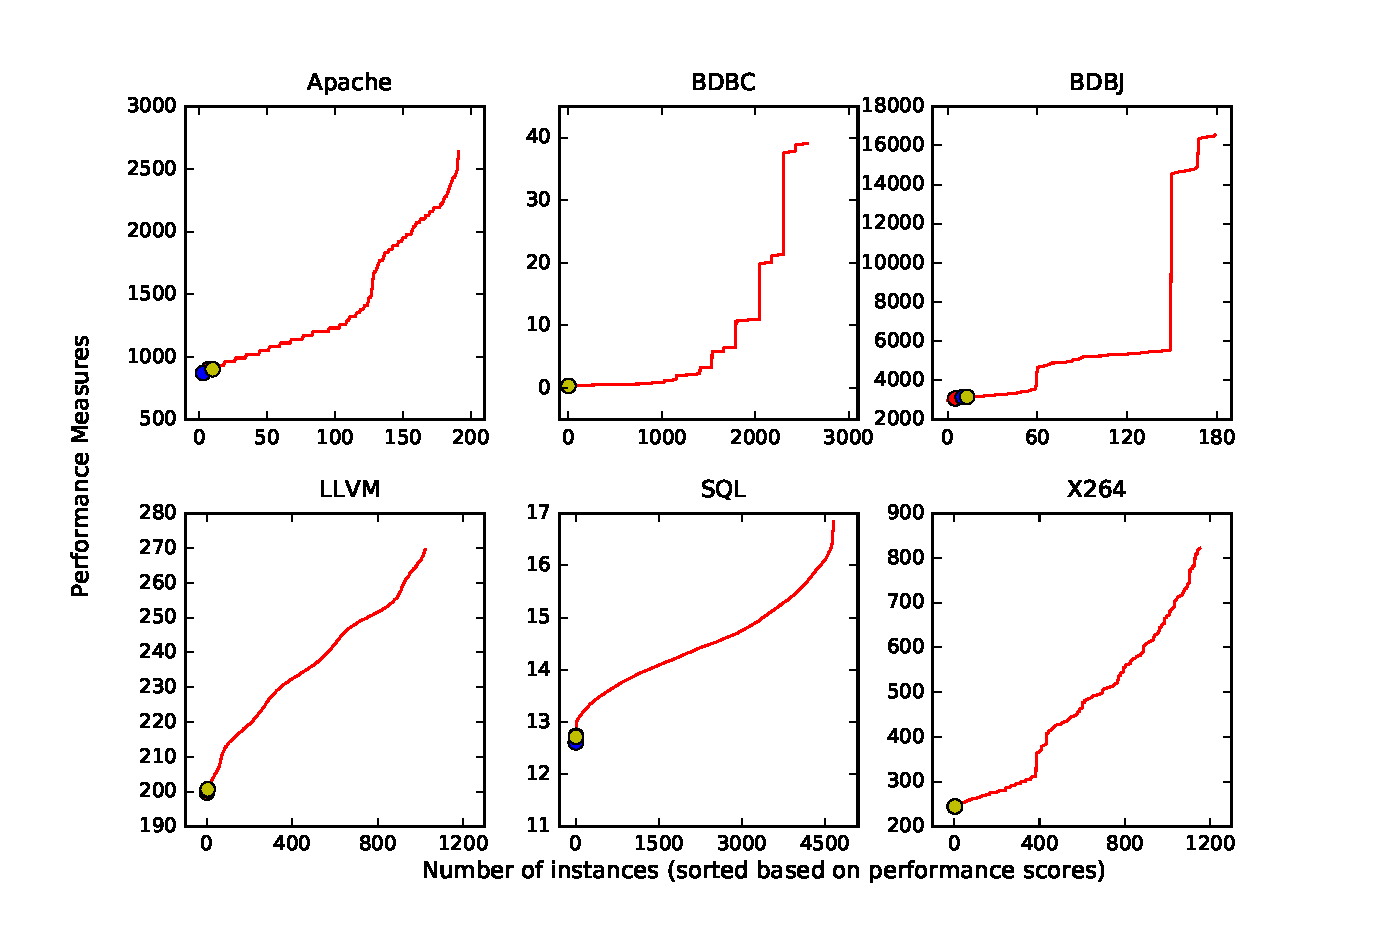
\includegraphics[width=\columnwidth]{Figures/optimizer_result}
\caption[Solutions found by GALE, NSGA-II and DE.]{Solutions found by GALE, NSGA-II and DE (shown as points) laid against the ground truth (all known configuration performance scores). 
% In case of Apache and BDBJ, we can see that the different optimizers find different solutions but in the remaining plots, the results are the same. 
It can be observed that all the optimizers can find the configuration with  lower performance scores.}\label{fig:performance_graph}
\end{figure}


The important feature of \fig{performance_graph} is that all the optimized configurations fall within 1\,\% of the fastest
configuration according to the ground truth (see all the left-hand-side dots on each plot). Table~\ref{fig:external_validity} compares the performance of the optimizers
used in this study. Note that the performances are nearly identical, which leads to the following conclusions:

\begin{myshadowbox}
The answer to {\bf RQ3} is ``yes'': For optimizing performance scores, we can use surrogates built from few runtime samples. The choice of the optimizer does not critically effect this conclusion.
\end{myshadowbox}


\begin{table}[tbh]
\centering
\caption[Minimum performance scores as found by the learners GALE, NSGA-II, and DE.]{The table shows how the minimum performance scores as found by the learners GALE, NSGA-II, and DE, vary over 20 repeated
runs. Mean values are denoted $\mu$ and IQR denotes the 25th--75th percentile. A low IQR suggests that the surrogate model build by \what is stable and can be utilized by off the shelf optimizers to find performance-optimal configurations.
% \todo[inline]{$\mu$ is reserved for the mean of the entire population, not for the mean of the part of the data we look at.}
}
\label{fig:external_validity}
\vspace{2ex}
\begin{tabular}{lrrrrrr}
\toprule
\multirow{3}{*}{\textbf{Dataset}} & \multicolumn{6}{c}{\textbf{Searcher}}                                                                       \\ \cmidrule{2-7} 
                                  & \multicolumn{2}{c}{\textbf{GALE}} & \multicolumn{2}{c}{\textbf{DE}} & \multicolumn{2}{c}{\textbf{NSGAII}} \\ \cmidrule{2-7} 
                                  & \textbf{Mean}    & \textbf{IQR}    & \textbf{Mean}   & \textbf{IQR}   & \textbf{Mean}     & \textbf{IQR}     \\ \midrule
\textbf{Apache}                   & 870              & 0               & 840             & 0              & 840               & 0                \\ 
\textbf{BDBC}                     & 0.363            & 0.004           & 0.359           & 0.002          & 0.354             & 0.005            \\ 
\textbf{BDBJ}                     & 3139             & 70              & 3139            & 70             & 3139              & 70               \\ 
\textbf{LLVM}                     & 202              & 3.98            & 200             & 0              & 200               & 0                \\ 
\textbf{SQLite}                   & 13.1             & 0.241           & 13.1            & 0              & 13.1              & 0.406            \\ 
\textbf{X264}                     & 248              & 3.3             & 244             & 0.003          & 244               & 0.05             \\ \bottomrule
\end{tabular}
\end{table}

% \begin{figure*}[tbh]
% 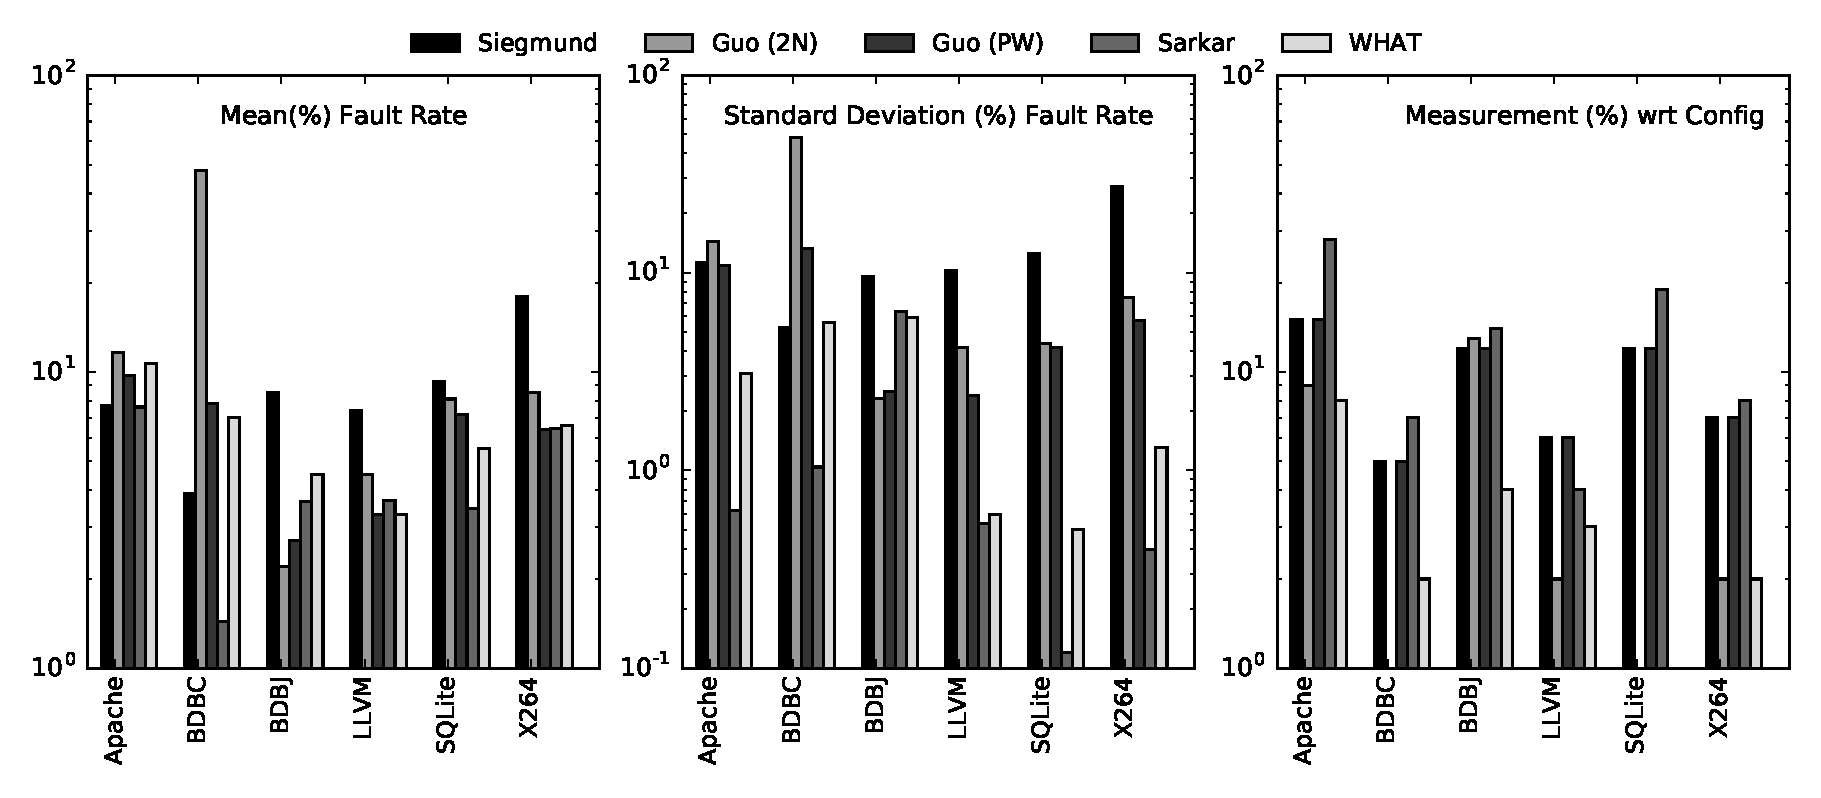
\includegraphics[width=\linewidth]{Figures/compare_graph_h}
% \caption{Comparison between \what and the state-of-the-art approaches regarding mean error, standard deviation, and the percentage of configurations used for training the model.} \label{fig:Comparison}
% % \todo[inline]{Please use different brightness/alpha values or patterns to be able to distinguish the bar on a print out.}
% \end{figure*}
 
 

 
 
\subsection{RQ4}


% \todo[inline]{change fault rate to error rate. note the sampling heuristic used for siegmund (I guess FW?!)}

 \begin{center}
{\em How good is \what compared to the state of the art of learning performance predictors from configurable software systems?}
\end{center}

We compare \what with the three state-of-the-art predictors proposed in the literature~\cite{siegmund2012predicting}, \cite{guo2013variability}, \cite{sarkar2015cost}, as discussed in Section~\ref{sect:addit}. Note that all approaches use regression-trees as predictors, except Siegmund's approach, which uses a regression function derived using linear programming.
The results were studied using non-parametric tests, which was also used by Arcuri and Briand at ICSE
'11~\cite{mittas13}). For testing statistical significance,
we used non-parametric bootstrap test 95\% confidence~\cite{efron93} followed by
an A12 test to check that any observed differences were not trivially small effects;
i.e. given two lists $X$ and $Y$, count how often there are larger
numbers in the former list (and there there are ties, add a half mark):
$a=\forall x\in X, y\in Y\frac{\#(x>y) + 0.5*\#(x=y)}{|X|*|Y|}$
(as per Vargha~\cite{Vargha00}, we say that a ``small'' effect has $a <0.6$). 
Lastly, to generate succinct reports, we use the Scott-Knott test to recursively
divide our optimizers. This recursion used A12 and bootstrapping  
to group together subsets that are (a)~not significantly different and are (b)~not
just a small effect different to each other. This use of Scott-Knott is endorsed
by Mittas and Angelis~\cite{mittas13}
and by Hassan et al.~\cite{7194626}.

\begin{figure}
 \begin{minipage}{4in}

        {\small
          \begin{tabular}{l@{~~~~}l@{~~~~}r@{~~~~}r@{~~}c@{}r}
    
    
  \multicolumn{1}{l}{\textbf{Rank}}& \textbf{using} & \textbf{Mean MRE}& \textbf{STDev} & \textbf{} & \textbf{Evaluations} \\ 
 \rowcolor{lightgray}\arrayrulecolor{lightgray}
\textbf{Apache}  & \textbf{} & \textbf{} & \textbf{}&\textbf{}&  \\\hline
  1 &       Sarkar &    7.49  &  0.82 & \quart{6}{3}{7} & 55 \\
  1 &      Guo(PW) &    10.51  &  6.85 & \quart{3}{33}{22} & 29 \\
  1 &     Siegmund &    10.34  &  11.68 & \quart{0}{55}{21} &  29\\
  1 &         	\textbf{WHAT} &    10.95  &  2.74 & \quart{16}{13}{24} & 16 \\
  1 &      Guo(2N) &    13.03  &  15.28 & \quart{7}{72}{34} &  18\\
\hline  
\rowcolor{lightgray}\arrayrulecolor{lightgray}
\textbf{BDBC}  & \textbf{} & \textbf{} & \textbf{}& \textbf{}&\\\hline
  1 &       Sarkar &    1.24  &  1.46 & \quart{0}{1}{0} &  191\\
\hline  2 &     Siegmund &    6.14  &  4.41 & \quart{4}{5}{6} &  139\\
  2 &         	\textbf{WHAT} &    6.57  &  7.4 & \quart{4}{9}{7} &  64\\
  2 &      Guo(PW) &    10.16  &  10.6 & \quart{2}{13}{11} &  139\\
\hline  3 &      Guo(2N) &    49.9  &  52.25 & \quart{16}{63}{59} &  36\\
\hline  
\rowcolor{lightgray}\arrayrulecolor{lightgray}
\textbf{BDBJ}  & \textbf{} & \textbf{} & \textbf{}& \textbf{}&\\\hline
  1 &      Guo(2N) &    2.29  &  3.26 & \quart{0}{29}{9} &  52\\
  1 &      Guo(PW) &    2.86  &  2.72 & \quart{2}{25}{14} &  48\\
  1 &         	\textbf{WHAT} &    4.75  &  4.46 & \quart{12}{40}{31} &  16\\
\hline  2 &       Sarkar &    5.67  &  6.97 & \quart{6}{62}{39} &  48\\
  2 &     Siegmund &    6.98  &  7.13 & \quart{16}{63}{51} &  57\\
\hline  
\rowcolor{lightgray}\arrayrulecolor{lightgray}
\textbf{LLVM}  & \textbf{} & \textbf{} & \textbf{}&\textbf{}& \\\hline
  1 &      Guo(PW) &    3.09  &  2.98 & \quart{0}{21}{10} &  64\\
  1 &         	\textbf{WHAT} &    3.32  &  1.05 & \quart{9}{7}{12} &  32\\
  1 &       Sarkar &    3.72  &  0.45 & \quart{13}{3}{15} &  62\\
  1 &      Guo(2N) &    4.99  &  5.05 & \quart{11}{36}{24} &  22\\
\hline  2 &     Siegmund &    8.5  &  8.28 & \quart{21}{58}{49} &  43\\
\hline
 
 
\rowcolor{lightgray}\arrayrulecolor{lightgray}
\textbf{SQLite} & \textbf{} & \textbf{} & \textbf{} & \textbf{}&\\\hline
  1 &       Sarkar &    3.44  &  0.1 & \quart{0}{0}{0} &  925\\
\hline  2 &         	\textbf{WHAT} &    5.6  &  0.57 & \quart{7}{2}{8} &  64\\
\hline  3 &      Guo(2N) &    8.57  &  7.3 & \quart{2}{28}{19} &  78\\
  3 &      Guo(PW) &    8.94  &  6.24 & \quart{6}{24}{20} &  566\\
\hline  4 &     Siegmund &    12.83  &  17.0 & \quart{16}{63}{35} &  566\\
\hline  
\rowcolor{lightgray}\arrayrulecolor{lightgray}
\textbf{x264} & \textbf{} & \textbf{} & \textbf{}& \textbf{}&\\\hline
  1 &       Sarkar &    6.64  &  1.04 & \quart{4}{2}{5} &  93\\
  1 &         	\textbf{WHAT} &    6.93  &  1.67 & \quart{4}{4}{6} &  32\\
  1 &      Guo(2N) &    7.18  &  7.07 & \quart{0}{15}{6} &  32\\
  1 &      Guo(PW) &    7.72  &  2.33 & \quart{4}{5}{8} &  81\\
\hline  2 &     Siegmund &    31.87  &  21.24 & \quart{32}{47}{61} &  81\\
\hline 

  \end{tabular}} 
\end{minipage}
\caption[Statistic tests comparing \what with different methods.]{Mean MRE seen in 20 repeats. Mean MRE is the prediction error as described in Equation~\ref{eq:err} and STDev is the standard deviation of the MREs found during multiple repeats. 
Lines with a a dot in the middle 
(e.g. \protect \quartex{3}{13}{13}) 
show the mean as a round dot withing the IQR (and if the IQR is very small, only a  round dot will be visible). 
All the results are sorted by the mean values: lower mean value of MRE is better than large mean value. 
The left-hand side columns \textbf{Rank} the various techniques, smaller the value of \textbf{Rank} better the technique e.g. in Apache, all the techniques have the same rank since their mean values are not statistically different. \textbf{Rank} is computer using Scott-Knott, bootstrap 95\% confidence, and the A12 test.
}
\label{fig:stats}
\end{figure} 

As seen in the Figure~\ref{fig:stats}, the FW approach of Siegmund et al. (i.e., the sampling approach using the fewest number of configurations) $(4/6)$ times has the higher errors rate and the highest standard deviation on that error rate. Hence, we cannot recommend this method or, if one wishes to use this method, we recommend using the other sampling heuristics (e.g., HO, HS) to make more accurate predictions (but at the cost of much more measurements). Moreover, the size of the standard deviation of this method causes further difficulties in estimating which configurations are those exhibiting a large prediction error. 

THere are two cases in Figure~\ref{fig:stats} where \what performs worse than at least one
other methods:
\begin{itemize}
\item 
SQLite: here, the Sukar methods does better that \what (3.44 vs 5.6)
but, as shown in the final column of Figure~\ref{fig:stats},
does so at the cost of $\frac{925}{64} \approx 15$ times more evaluations that \what.
In this case, a pragmatic engineering could well prefer our solution the that of Sukar (since
Sukar uses  more than an order of magnitude slowdown).
\item BDBC: Here again, \what is not doing the best but, compared to the space of
all other solutions, it  is not doing particular bad.
\end{itemize}


As to the approach of Guo et al (with PW), this does not standout on any of our measurements. Its error results are within 1\% of \what; its standard deviation are usually larger and it requires much more data than \what (Evaluations column of the figure). 

In terms of the number of measure samples required to build a model, the right-hand most column of Figure~\ref{fig:stats} shows that \what requires the fewest samples except for two cases: the approach of Guo et al. (with 2N) working on BDBC and LLVM. In both these cases, the mean error and standard deviation on the error estimate is larger than \what. Furthermore, in the case of BDBC, the error values
 are $\mu=14\,\%$, $\sigma=13\,\%$, which are much larger
than \what{}'s error scores of $\mu=6\,\%$, $\sigma=5\,\%$.

Although the approach of Sarkar et al. produces an error rate that is sometimes less than the one of \what, it requires the most number of measurements. Moreover, \what\'s  accuracy is close to Sarkar\'s approach (1\% to 2\%) difference). Hence, we cannot recommend this approach, too.

Table~\ref{tab:measurements} shows the number of evaluations used by each approaches. We see that most state-of-the-art approaches often require many more samples than
\what{}.  Using those fewest numbers of samples, \what has
within 1 to 2\,\% of the lowest standard deviation rates 
and within 1 to 2\,\% of lowest error rates.
The exception is Sarkar's approach, which has 5\,\% lower mean error
rates.  However, 
as shown in right-hand-side of Table~\ref{tab:measurements}, Sarkar's approach needs nearly three times
more measurements than \what (191 vs 64 samples). Given
the overall reduction of the error is   small (5\,\% difference
between Sarkar and \what in mean error), the overall
cost of tripling the data-collection cost is
often not feasible in a practical context and might not justify the small additional benefit in accuracy. 

%  The \framebox{\colorbox{whatcolor}{\textcolor{whatcolor}{\bf blue}}} bars of Figure \ref{fig:Comparison} show the
%  mean error rate, the standard deviation of the error rate, and the mean percentage
%  of total configurations used in 30 repeats of the different approaches.
%  Note that the y-axis of that figure is a logarithmic scale so, within each plot:
%  \begin{itemize}
%  \item Differences near the bottom  are very small differences;
%  \item Differences near the top   are very large differences;
%  \end{itemize}
 
% As seen in the left and middle plots of
% Figure~\ref{fig:Comparison}, 
% the {\em FW} approach of Siegmund et al.\ (i.e., the sampling approach using the fewest number of configurations) often has the highest
% error rate and the highest
% standard deviation on that error rate. Hence,
% we cannot recommend this method or,  if one wishes to use this method, we recommend using the other sampling heuristics (e.g., HO, HS) to make more accurate predictions (but at the cost of much more measurements). Moreover, the size of the standard deviation of this method causes further difficulties in estimating which configurations are those exhibiting a large prediction error. 

% As to the approach of Guo et al.\ (with PW), this   does not standout on any of
% our measurements. Its error results are within 1\,\% of \what;
%  its standard deviation are usually larger; and it requires
%  much more data than \what.
 
%  In terms of the number of measured samples required to build a model, 
%  the right-hand-side plot of  Figure~\ref{fig:Comparison}  shows that
%  \what requires the fewest samples except for two cases:
%  the approach of Guo et al. (with 2N) working on BDBC and LLVM.  In both these cases, the mean error and standard deviation on the error
%  estimate is   larger than \what  (see the \framebox{\colorbox{guocolor}{\textcolor{guocolor}{\bf red}}} bars in the left and middle plots   of Figure~\ref{fig:Comparison}). Furthermore, in the case of BDBC, the error values
%  are $\mu=14\,\%$, $\sigma=13\,\%$, which are much larger
% than \what{}'s error scores of $\mu=6\,\%$, $\sigma=5\,\%$. 


% Although the approach of Sarkar et al.\ produces an error rate that is sometimes less than the one of \what (see the left-hand-side of
% Figure~\ref{fig:Comparison}), it requires the most number of measurements. Moreover, \what's accuracy is close to Sarkar's approach (1\,\%
% to 2\,\% difference). Hence, we cannot recommend this approach, too.

% %Nor can we recommend the approach of Sarkar et al.\ since,
% %as shown on the right-hand-side of Figure~\ref{fig:Comparison}, 
% %this approach requires the most data.
% %While it is true that its error rate 
% %is sometimes less than the one of \what (see the left-hand-side of
% %Figure~\ref{fig:Comparison}), that difference is often small (1\,\%
% %to 2\,\%). 

% %The exception here is BDBC, where Sarker's approach has the lowest
% %error of any approach. This exception is discussed further in the
% %next paragraph.
 

% The right-hand-side of Figure~\ref{fig:Comparison}   shows
% the {\em percent} of required measurements. Table~\ref{tab:measurements} shows the same
% expressed as absolute values. We see that most state-of-the-art approaches often require many more samples than
% \what{}.  Using those fewest numbers of samples, \what has
% within 1 to 2\,\% of the lowest standard deviation rates 
% and within 1 to 2\,\% of lowest error rates.
% The exception is Sarkar's approach, which has 5\,\% lower mean error
% rates (in BDBC, see the left-hand-side plot of Figure~\ref{fig:Comparison}).  However, 
% as shown in right-hand-side of Table~\ref{tab:measurements}, Sarkar's approach needs nearly three times
% more measurements than \what (191 vs 64 samples). Given
% the overall reduction of the error is   small (5\,\% difference
% between Sarkar and \what in mean error), the overall
% cost of tripling the data-collection cost is
% often not feasible in a practical context and might not justify the small additional benefit in accuracy. 


 %Note that:
%  \bi
%     \item
    
%  \ei




\begin{table}[t]
\caption[Comparison of the number of the samples
required by \what with the state of the art]{Comparison of the number of the samples
required with the state of the art. The grey colored cells indicate the approach which has the lowest number of samples.  We notice that WHAT and Guo (2N) uses less data compared to other approaches. The high fault rate  of Guo (2N) accompanied with high variability in the predictions makes WHAT our preferred method.}\label{tab:measurements}
\vspace{2ex}
\centering
\small
\begin{tabular}{lrrrrr}
\toprule
                                   & \multicolumn{5}{c}{\textbf{Samples}}                                                                         \\ \cmidrule{2-6} 
\multirow{-2}{*}{\textbf{Dataset}} & \textbf{Siegmund} & \textbf{Guo (2N)}          & \textbf{Guo (PW)} & \textbf{Sarkar} & \textbf{\what}                \\ \midrule
\textbf{Apache}                    & 29                & 181                        & 29                & 55              & \cellcolor[HTML]{C0C0C0}16 \\ 
\textbf{BDBC}                      & 139               & \cellcolor[HTML]{C0C0C0}36 & 139               & 191             & 64                         \\ 
\textbf{BDBJ}                      & 48                & 52                         & 48                & 57              & \cellcolor[HTML]{C0C0C0}16 \\ 
\textbf{LLVM}                      & 62                & \cellcolor[HTML]{C0C0C0}22 & 64                & 43              & 32                         \\ 
\textbf{SQLite}                    & 566               & 78                         & 566               & 925             & \cellcolor[HTML]{C0C0C0}64 \\ 
\textbf{X264}                      & 81                & \cellcolor[HTML]{C0C0C0}32 & 81                & 93              & \cellcolor[HTML]{C0C0C0}32 \\ \bottomrule
\end{tabular}
\end{table}

% % Please add the following required packages to your document preamble:
% \usepackage{multirow}
% \usepackage[table,xcdraw]{xcolor}
% If you use beamer only pass "xcolor=table" option, i.e. \documentclass[xcolor=table]{beamer}
\begin{figure*}[!t]
\centering
\begin{tabular}{|l|l|l|l|l|l|l|l|}
\hline
                                   & \multicolumn{2}{c|}{}                                             &                                            & \multicolumn{2}{l|}{\thead{FaultRate(Them) \\ Siegmund et al.}}               & \multicolumn{2}{l|}{\thead{FaultRate(US) \\ This paper}}   \\ \cline{5-8} 
\multirow{-2}{*}{\thead{Dataset}} & \multicolumn{2}{c|}{\multirow{-2}{*}{\thead{Measurement(Them) \\ Siegmund et al. \\}}} & \multirow{-2}{*}{\thead{Measurement(Us) \\ This paper \\}} & \thead{Mean}                & \thead{Std}                 & \thead{Mean}         & \thead{Std}          \\ \hline
                                   & FW                              & 15                              &                                            & \cellcolor[HTML]{C0C0C0}44.1 & \cellcolor[HTML]{C0C0C0}42.3 &                       &                       \\ \cline{2-3} \cline{5-6}
                                   & PW                              & \cellcolor[HTML]{FD6864}139                             &                                            & 3.9                          & 5.3                          &                       &                       \\ \cline{2-3} \cline{5-6}
                                   & HO                              & \cellcolor[HTML]{FD6864}160                             &                                            & 2.8                          & 3.7                          &                       &                       \\ \cline{2-3} \cline{5-6}
\multirow{-4}{*}{BDBC}             & HS                              & \cellcolor[HTML]{FD6864}164                             & \multirow{-4}{*}{64}                       & 2.8                          & 3.7                          & \multirow{-4}{*}{9.3} & \multirow{-4}{*}{6.8} \\ \hline
                                   & FW                              & 10                              &                                            & \cellcolor[HTML]{C0C0C0}17.7 & \cellcolor[HTML]{C0C0C0}19.6 &                       &                       \\ \cline{2-3} \cline{5-6}
                                   & PW                              & 48                              &                                            & \cellcolor[HTML]{C0C0C0}8.5  & \cellcolor[HTML]{C0C0C0}9.6  &                       &                       \\ \cline{2-3} \cline{5-6}
                                   & HO                              & \cellcolor[HTML]{FD6864}116                             &                                            & \cellcolor[HTML]{C0C0C0}3.8  & \cellcolor[HTML]{C0C0C0}5.7  &                       &                       \\ \cline{2-3} \cline{5-6}
\multirow{-4}{*}{BDBJ}             & HS                              & \cellcolor[HTML]{FD6864}162                             & \multirow{-4}{*}{64}                       & 1.7                          & 3.5                          & \multirow{-4}{*}{2.7} & \multirow{-4}{*}{0.7} \\ \hline
                                   & FW                              & 9                               &                                            & \cellcolor[HTML]{C0C0C0}14.9 & \cellcolor[HTML]{C0C0C0}24.8 &                       &                       \\ \cline{2-3} \cline{5-6}
                                   & PW                              & \cellcolor[HTML]{FD6864}29                              &                                            & \cellcolor[HTML]{C0C0C0}7.7  & \cellcolor[HTML]{C0C0C0}11.2 &                       &                       \\ \cline{2-3} \cline{5-6}
                                   & HO                              & \cellcolor[HTML]{FD6864}80                              &                                            & \cellcolor[HTML]{C0C0C0}11.6 & \cellcolor[HTML]{C0C0C0}22.7 &                       &                       \\ \cline{2-3} \cline{5-6}
\multirow{-4}{*}{Apache}           & HS                              & \cellcolor[HTML]{FD6864}143                             & \multirow{-4}{*}{16}                       & 5.3                          & 10.8                         & \multirow{-4}{*}{9.9} & \multirow{-4}{*}{2.4} \\ \hline
                                   & FW                              & 26                              &                                            & \cellcolor[HTML]{C0C0C0}7.8  & \cellcolor[HTML]{C0C0C0}9.2  &                       &                       \\ \cline{2-3} \cline{5-6}
                                   & PW                              & \cellcolor[HTML]{FD6864}566                             &                                            & \cellcolor[HTML]{C0C0C0}9.3  & \cellcolor[HTML]{C0C0C0}12.5 &                       &                       \\ \cline{2-3} \cline{5-6}
                                   & HO                              & \cellcolor[HTML]{FD6864}566                             &                                            & \cellcolor[HTML]{C0C0C0}7.1  & \cellcolor[HTML]{C0C0C0}9.1  &                       &                       \\ \cline{2-3} \cline{5-6}
\multirow{-4}{*}{SQL}              & HS                              & \cellcolor[HTML]{FD6864}569                             & \multirow{-4}{*}{64}                       & \cellcolor[HTML]{C0C0C0}7    & \cellcolor[HTML]{C0C0C0}9    & \multirow{-4}{*}{5.6} & \multirow{-4}{*}{0.2} \\ \hline
                                   & FW                              & 11                              &                                            & \cellcolor[HTML]{C0C0C0}7.8  & \cellcolor[HTML]{C0C0C0}9    &                       &                       \\ \cline{2-3} \cline{5-6}
                                   & PW                              & \cellcolor[HTML]{FD6864}62                              &                                            & \cellcolor[HTML]{C0C0C0}7.4  & \cellcolor[HTML]{C0C0C0}10.2 &                       &                       \\ \cline{2-3} \cline{5-6}
                                   & HO                              & \cellcolor[HTML]{FD6864}62                              &                                            & \cellcolor[HTML]{C0C0C0}7.4  & \cellcolor[HTML]{C0C0C0}10.2 &                       &                       \\ \cline{2-3} \cline{5-6}
\multirow{-4}{*}{LLVM}             & HS                              & \cellcolor[HTML]{FD6864}88                              & \multirow{-4}{*}{32}                       & \cellcolor[HTML]{C0C0C0}5.7  & \cellcolor[HTML]{C0C0C0}7    & \multirow{-4}{*}{3.3} & \multirow{-4}{*}{0.3} \\ \hline
                                   & FW                              & 12                              &                                            & \cellcolor[HTML]{C0C0C0}29.8 & \cellcolor[HTML]{C0C0C0}22   &                       &                       \\ \cline{2-3} \cline{5-6}
                                   & PW                              & \cellcolor[HTML]{FD6864}81                              &                                            & \cellcolor[HTML]{C0C0C0}17.9 & \cellcolor[HTML]{C0C0C0}27.2 &                       &                       \\ \cline{2-3} \cline{5-6}
                                   & HO                              & \cellcolor[HTML]{FD6864}89                              &                                            & 5.1                          & 15.1                         &                       &                       \\ \cline{2-3} \cline{5-6}
\multirow{-4}{*}{x264}             & HS                              & \cellcolor[HTML]{FD6864}89                              & \multirow{-4}{*}{32}                       & 5.1                          & 15.1                         & \multirow{-4}{*}{6.6} & \multirow{-4}{*}{0.5} \\ \hline
\end{tabular}
\caption{Comparison of
Seigmund et.al \cite{siegmund2012predicting} with WHAT+$S_1$:Random 
(shown in right-hand columns). Gray   denote cases where prior work has larger median error. Red test denotes all cases where prior work used large samples. Note that in all cases where prior work achieved lower mean error rate, they required more samples for ex. in Apache HS 143 samples to 16 samples with our method.
}\label{fig:vs2012}
\end{figure*}

% % Please add the following required packages to your document preamble:
% \usepackage[table,xcdraw]{xcolor}
% If you use beamer only pass "xcolor=table" option, i.e. \documentclass[xcolor=table]{beamer}
\begin{figure*}[!t]
\centering
\begin{tabular}{|l|l|l|l|l|l|l|}
\hline
\thead{Dataset} & \thead{Mean Fault \\ Rate(Guo)} & \thead{Standard \\ Deviation(Guo)}   & \thead{Measurement \\ (Guo)} & \thead{Mean Fault \\ Rate(Us)} & \thead{Standard \\ Deviation(Us)} & \thead{Measurement \\ (Us)} \\ \hline
\textbf{Apache}  & \cellcolor[HTML]{C0C0C0}11.6  & \cellcolor[HTML]{C0C0C0}14.4  & \cellcolor[HTML]{C0C0C0}18 & 9.9                          & 2.4                         & 16                         \\ \hline
\textbf{LLVM}    & \cellcolor[HTML]{C0C0C0}4.5   & \cellcolor[HTML]{C0C0C0}4.2   & 22                         & 3.3                          & 0.3                         & 32                         \\ \hline
\textbf{X264}    & \cellcolor[HTML]{C0C0C0}8.5   & \cellcolor[HTML]{C0C0C0}7.5   & \cellcolor[HTML]{C0C0C0}32 & 6.6                          & 0.5                         & 32                         \\ \hline
\textbf{BDBC}    & \cellcolor[HTML]{C0C0C0}98.3  & \cellcolor[HTML]{C0C0C0}243.1 & 36                         & 9.3                          & 6.8                         & 64                         \\ \hline
\textbf{BDBJ}    & 2.2                           & \cellcolor[HTML]{C0C0C0}2.3   & 52                         & 2.7                          & 0.7                         & 64                         \\ \hline
\textbf{SQLite}  & \cellcolor[HTML]{C0C0C0}8.1   & \cellcolor[HTML]{C0C0C0}4.4   & \cellcolor[HTML]{C0C0C0}78 & 5.6                          & 0.2                         & 64                         \\ \hline
\end{tabular}
\caption{Comparison of
Guo et.al \cite{guo2013variability}, which uses $2*N$ number of configurations with WHAT + $S_1$ 
(shown in right-hand columns). Here N refers to the number of features of the software system (please refer to \cite{guo2013variability} for more details).  Gray denotes the cases where our method results in lower median fault rate and is more stable i.e. lower standard deviation. We see that our method does better in 3 out of 6 datasets. }\label{fig:guo_2n}
\end{figure*}

% % Please add the following required packages to your document preamble:
% \usepackage[table,xcdraw]{xcolor}
% If you use beamer only pass "xcolor=table" option, i.e. \documentclass[xcolor=table]{beamer}
\begin{figure*}[!t]
\centering
\begin{tabular}{|l|l|l|l|l|l|l|}
\hline
\thead{Dataset} & \thead{Mean Fault \\ Rate(Guo)} & \thead{Standard \\ Deviation(Guo)}   & \thead{Measurement \\ (Guo)} & \thead{Mean Fault \\ Rate(Us)} & \thead{Standard \\ Deviation(Us)} & \thead{Measurement \\ (Us)} \\ \hline
\textbf{Apache}  & 9.7                           & \cellcolor[HTML]{C0C0C0}10.8 & \cellcolor[HTML]{C0C0C0}29  & 9.9                          & 2.4                         & 16                         \\ \hline
\textbf{LLVM}    & 3.3                           & \cellcolor[HTML]{C0C0C0}2.4  & \cellcolor[HTML]{C0C0C0}64  & 3.3                          & 0.3                         & 32                         \\ \hline
\textbf{X264}    & 6.4                           & \cellcolor[HTML]{C0C0C0}5.7  & \cellcolor[HTML]{C0C0C0}81  & 6.6                          & 0.5                         & 32                         \\ \hline
\textbf{BDBC}    & 7.8                           & \cellcolor[HTML]{C0C0C0}13.2 & \cellcolor[HTML]{C0C0C0}139 & 9.3                          & 6.8                         & 64                         \\ \hline
\textbf{BDBJ}   * & 2.7                           & \cellcolor[HTML]{C0C0C0}2.5  & 48                          & 2.7                          & 0.7                         & 64                         \\ \hline
\textbf{SQLite}  & \cellcolor[HTML]{C0C0C0}7.2   & \cellcolor[HTML]{C0C0C0}4.2  & \cellcolor[HTML]{C0C0C0}566 & 5.6                          & 0.2                         & 64                         \\ \hline
\end{tabular}
\caption{Comparison of
Guo et.al \cite{guo2013variability} with PW number of configurations with WHAT+$S_1$ 
(shown in right-hand columns). Here N refers to the number of features of the software system (please refer to \cite{guo2013variability} for more details). Gray denotes the cases where our method results in lower median fault rate and is more stable i.e. lower standard deviation. We see that our method does better in SQLite and close to prior works results using far less evaluation (except for BDBC).}\label{fig:guo_pw}
\end{figure*}

% \begin{figure*}[!t]
\centering
\begin{tabular}{|l|l|l|l|l|l|l|}
\hline
                                   & \multicolumn{3}{l|}{\textbf{Their}}                                                                                                                                                                                                  & \multicolumn{3}{l|}{\textbf{Us}}                                                                                                                                                                                           \\ \cline{2-7} 
\multirow{-2}{*}{\textbf{Dataset}} & \textbf{\begin{tabular}[c]{@{}l@{}}Mean Fault\\ Rate(Sarkar)\end{tabular}} & \textbf{\begin{tabular}[c]{@{}l@{}}Standard\\ Deviation(Sarkar)\end{tabular}} & \textbf{\begin{tabular}[c]{@{}l@{}}Measurement\\ (Sarkar)\end{tabular}} & \textbf{\begin{tabular}[c]{@{}l@{}}Mean Fault\\ Rate (Us)\end{tabular}} & \textbf{\begin{tabular}[c]{@{}l@{}}Standard\\ Deviation (Us)\end{tabular}} & \textbf{\begin{tabular}[c]{@{}l@{}}Measurement\\ (Us)\end{tabular}} \\ \hline
Apache                             & 7.61                                                                       & 0.63                                                                          & \cellcolor[HTML]{FD6864}55                                              & 9.9                                                                     & 2.4                                                                        & 16                                                                  \\ \hline
BDBC                               & 1.44                                                                       & 1.04                                                                          & \cellcolor[HTML]{FD6864}191                                             & 9.3                                                                     & 6.8                                                                        & 64                                                                  \\ \hline
BDBJ                               & \cellcolor[HTML]{C0C0C0}3.66                                               & \cellcolor[HTML]{C0C0C0}6.34                                                  & 57                                                                      & 2.7                                                                     & 0.7                                                                        & 64                                                                  \\ \hline
LLVM                               & \cellcolor[HTML]{C0C0C0}3.67                                               & \cellcolor[HTML]{C0C0C0}0.55                                                  & \cellcolor[HTML]{FD6864}43                                              & 3.3                                                                     & 0.3                                                                        & 32                                                                  \\ \hline
SQLite                             & 3.46                                                                       & 0.08                                                                          & \cellcolor[HTML]{FD6864}925                                             & 5.6                                                                     & 0.2                                                                        & 64                                                                  \\ \hline
X264                               & 6.43                                                                       & \cellcolor[HTML]{C0C0C0}0.4                                                   & \cellcolor[HTML]{FD6864}93                                              & 6.6                                                                     & 0.5                                                                        & 32                                                                  \\ \hline
\end{tabular}
\caption{
Comparison of
Sarkar et.al's \cite{sarkar2015cost} recommended method (projective sampling)  with  \what +$S_1$ 
(shown in right-hand columns). Gray denotes the cases where our method results in lower median fault rate and is more stable i.e. lower standard deviation. We see that out method performs almost similar (LLVM and X264) and sometime better (BDBJ). The cases where we see that Sarkar et. al's method works better than \what, they use any where between 3 ( Apache, BDBC) to 14 (SQLite) times more points.
} \label{fig:sarkar}
\end{figure*}

% \fig{vs2012} compares the errors found by  \what+ $S_1$:Random with those found by the minimal sampling
% methods from Siegmund et al. Note that:
% \bi
% \item
% Simple feature-wise (FW) sampling uses fewer samples that 
% other methods, but its mean error and/or standard deviation can be largest. Hence, a simple addition
% of the known performance scores for individual features is less reliable that the other methods.
% \item
% As to the other minimal sampling methods  (PW,HO,HS)  \what+$S_1$:Random always had a   lower mean
% error rate and a much lower standard deviation on the error.  
% \item In terms of number of samples required to make those predictions, \what+$S_1$:Random needed
% much less detail that PW or HO or HS
% \ei


% Guo et al. proposed progressively random sampling methodology which samples in steps of the number of features in the software system. The termination criteria of this technique is based on the heuristic called as $PW$ same as the one described in  Siegmund et al.

% \fig{guo_2n} compares the errors found by  \what+ $S_1$:Random with those found by the minimal sampling
% methods when it used $2*N$ samples. The number of configurations evaluated is very close to the  number of configurations evaluated by our method.

% \fig{guo_pw} compares the errors found by  \what+ $S_1$:Random with those found by the progressive sampling method  after allowing it to run till completion.

% Note that: 
% \bi
% \item
% Comparing the numbers in \fig{guo_2n}, our method is better than Guo et al. sampling method in terms of higher accuracy and lower standard deviation (more stability). When comparing numbers in the \fig{guo_pw} our method is very close to the mean fault rate (except for BDBJ) but significantly better in terms of stability and number of measurements especially in case SQLite.
% \item
% The results are a clear indication that random sampling in itself is not a good policy where as exploiting the underlying dimension (uses spectral clustering) can generate more accurate and stable predictors
% \ei


\begin{myshadowbox}
Hence, we answer {\bf RQ4} with ``yes'',
since \what yields predictions that are similar to or more accurate than prior
work, while requiring fewer samples.
\end{myshadowbox}

\section{Why does it work?}
In this section, we present an in-depth analysis to understand why our sampling technique (based on a spectral learner) achieves such low mean fault rates while being stable (low variance). We hypothesize that the configuration space of the system configuration lie on a low dimensional manifold. 

\subsection{History}
Menzies et. al~\cite{me12d} suggested data heterogeneity by demonstrating the existence of local regions, which were very different from the global representation. Menzies et al. also makes an important observation about exploiting the underlying dimension to cluster the data. The authors used an algorithm called WHERE (see section~\ref{rtlearning}), which recurses on two dimensions synthesized in linear time using a technique called FASTMAP~\cite{faloutsos1995fastmap}. The use of underlying dimension has been endorsed by various other researchers~\cite{bettenburg2012think, deiters2013using, bettenburg2015towards, zhang2016cross}. There are numerous other methods in the literature, which are used to learn the underlying dimensionality of the data set like Principal Component Analysis (PCA)~\cite{jolliffe2002principal}~\footnote{WHERE is an approximation of the first principal component}, Spectral Learning~\cite{shi00}, Random Projection~\cite{bingham2001random}.  These algorithms  use  different techniques to identify the underlying, independent/orthogonal dimensions to cluster the data points and differ with respect to the computational complexity and accuracy. We use WHERE since it computationally efficient~$O(2N)$ while being accurate.



\subsection{Testing Technique}
Given our hypothesis -- configuration space lies in a lower dimensional hyperplane--  it is imperative to demonstrate that the intrinsic dimensionality of the configuration space is less than actual dimension. To formalize this notion we borrow the concept of correlation dimension from the domain of physics~\cite{grassberger2004measuring}. The correlation dimension of a dataset with $k$ item is found by computing the number of items found at distance withing radius $r$ (where r is the euclidean distance between two configurations) while varying $r$. This is then normalized by the number of connections between $k$ items to find the expected number of neighbors at distance $r$. This can be written as:
\begin{equation}
    C(r) = \frac{2}{k(k-1)} \displaystyle\sum_{i=1}^{n} \displaystyle\sum_{j=i+1}^{n} I(||x_i, x_j|| < r) \\  
 \end{equation} 
$$
where:
    I(x < y) = \begin{cases}
            1, & \text{ if x \textless y}\\
            0, & \text{ otherwise}\\
    \end{cases}
$$
  

Given the dataset with $k$ items and range of distances [$r_0$--$r_{max}$], we estimate the intrinsic dimensionality as the maximum slope between $\ln(C(r))$ vs $\ln(r)$.

\subsection{Evaluation}
\begin{figure}[t]
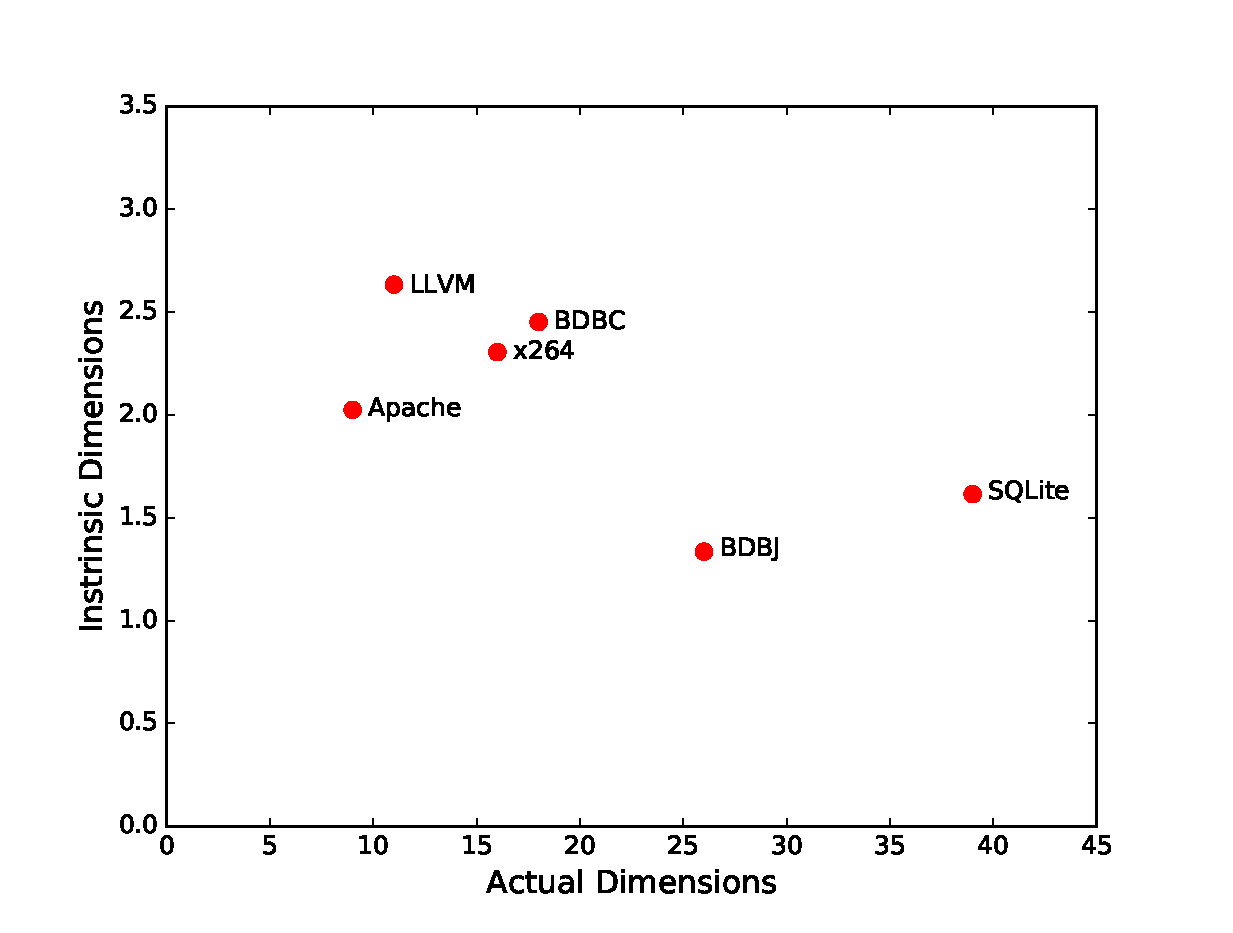
\includegraphics[width=0.9\columnwidth]{Figures/underlying_dimension}
\caption[Intrinsic dimensionality of the subjects systems.]{Intrinsic dimensionality of the subjects systems are shown on the y-axis. The number on the side is the actual dimension of the system. The intrinsic dimensionality of the systems are much lower than the actual dimensionality (number of columns in the dataset).}
\label{fig:underlying_d}
\end{figure}
We observe that \textbf{the intrinsic dimensionality of the software system is much lower than the actual dimension}. Figure \ref{fig:underlying_d} presents the intrinsic dimensionality along with the actual dimensions of the software systems. If we take a look at the intrinsic dimensionality and compare it with the actual dimensionality, then it becomes apparent that the configuration space lies on a lower dimensional hyperplane. For example, SQLite has 39 configuration options but the intrinsic dimensionality of the space is just 7.61 (this is a fractal dimension). At the heart of \what is WHERE (a spectral clusterer), which uses the approximation of the first principal component to divide the configuration space and hence can take advantage of the low intrinsic dimensionality. 

As a summary, our observations indicates that the intrinsic dimension of the configuration space is much lower that its actual dimension. Hence, clustering based on the intrinsic dimensions rather than the actual dimension would be more effective. In other words, configurations with similar performance values lie closer in the intrinsic hyperplane when compared to the actual dimensions and may be the reason as to why \what achieves empirically good results.

\begin{myshadowbox}
The intrinsic dimension of the configuration space is much lower than its actual dimension and hence clustering based on the intrinsic dimension is more effective.
\end{myshadowbox}

\section{Reliability and Validity}\label{sect:construct}

{\em Reliability} refers to the consistency of the results obtained
from the research.  For example,   how well independent researchers
could reproduce the study? To increase external
reliability, this paper has taken care to either  clearly define our
algorithms or use implementations from the public domain
(SciKitLearn)~\cite{scikit-learn}. Also, all the data used in this work is available
on-line in the PROMISE code repository and all our algorithms
are on-line at github.com/ai-se/where.

{\em Validity} refers to the extent to which a piece of research actually
investigates what the researcher purports to investigate~\cite{SSA15}.
{\em Internal validity} checks if the differences found in
the treatments can be ascribed to the treatments under study. 

One internal validity issue with our experiments is the choice
of {\em training and testing} data sets discussed in 
\fig{systems}. Recall that while all our learners used the same
{\em testing} data set, our untuned learners were only given
access to {\em training} data.

Another internal validity issues is {\em instrumentation}. The very low $\mu$ and $\sigma$ error values
reported in this study are so small that it is reasonable to ask whether they are due to some instrumentation
quirk, rather than due to using a clever sample strategy:
\begin{itemize}
\item
Our low $\mu$ values are consistent with prior work (e.g.~\cite{sarkar2015cost});
\item
As to our low $\sigma$ values, we note that, when the  error values are so close to 0\,\%, the standard
deviation of the error is ``squeezed'' between zero and those errors. Hence, we would expect that
experimental rigs
that generate error values on the order of 5\,\% and \eq{err} should have $\sigma$ values of $0\le \sigma \le 5$ (e.g., like those seen in our introduction).
\end{itemize}

Regarding SQLite, we cannot measure all possible configurations in reasonable time. Hence, we sampled only 100 configurations to compare prediction and actual performance values. We are aware that this evaluation leaves room for outliers.
Also, we are aware that measurement bias can cause false interpretations~\cite{me12d}. Since we aim at predicting performance for a special workload, we do not have to vary benchmarks.



  We aimed at increasing the {\em external validity} by choosing software systems from different domains with different configuration mechanisms and implemented with different programming languages. Furthermore, the systems used are deployed and used in the real world. Nevertheless, assuming the evaluations to be automatically transferable  to all configurable software systems is not fair. To further strengthen external validity, we run the model (generated by \textit{\what + $S_1$}) against other optimizers, such as NSGA-II and differential evolution~\cite{storn1997differential}. That is, we validated whether the learned models are not only applicable for GALE style of perturbation. In Table~\ref{fig:external_validity}, we see that the models developed are valid for all optimizers, as all optimizers are able to find the near optimal solutions.



\section{Related Work}
\label{sect:related}
 
In 2000, Shi and Maik~\cite{shi00} claimed the term ``spectral clustering'' as a reference to their normalized cuts
image
segmentation algorithm that  partitions data through a spectral (eigenvalue) analysis of the  
Laplacian representation of the similarity graph between instances in the data.

In 2003, Kamvar et al.~\cite{kamvar2003spectral}  generalized that definition saying that ``spectral learners''
were any data-mining algorithm that first replaced the raw
dimensions with those inferred from the spectrum (eigenvalues) of the affinity (a.k.a.\ distance)
matrix of the data, optionally adjusted via some normalization technique).

Our clustering based on first principal component splits the data on a   approximation to an eigenvector, found at each recursive level
of the data (as described in \tion{spect}). 
Hence, this  method is a ``spectral clusterer'' in the general Kamvar sense. 
Note that,
for our data, we have
not found that Kamvar's normalization matrices are needed.

Regarding sampling, there are a wide range of methods know as experimental designs or designs of experiments~\cite{pukelsheim2006optimal}. They usually rely on fractional factorial designs as in the combinatorial testing community~\cite{Kuhn:2013}. 

Furthermore, there is a recent approach that learns {\em per\-for\-mance-influence models} for configurable software systems~\cite{SGA+15}. While this approach can handle even numeric features, it has similar sampling techniques for the Boolean features as reported in their earlier work~\cite{siegmund2012predicting}. Since we already compared to that earlier work and do not consider also numeric features, we did not compare our work to performance-influence models.
% (but perhaps if we were text mining
%on very large dimensional data, we would add in that normalization). 
 



\section{Conclusions}

Configurable software systems today are widely used in practice, but expose challenges
regarding finding performance-optimal configurations. State-of-the-art approaches require too
many measurements or are prone to large variances in their performance predictions. To avoid
these shortcomings, we have proposed a fast spectral learner, called \what,  along with three
new sampling techniques. The key idea of \what is to explore the configuration space with
eigenvalues of the features used in a configuration to determine exactly those configurations
for measurement that reveal key performance characteristics. 
This way, we can study many closely associated configurations with only a few measurements.

We evaluated our approach on six real-world configurable software systems borrowed from the
literature. Our approach achieves similar to lower error rates, while being stable when
compared to the state of the art. In particular, with the exception of Berkeley DB, our
approach is more accurate than the state-of-the-art approaches by Siegmund et
al.~\cite{siegmund2012predicting} and Guo et al.~\cite{guo2013variability}. Furthermore, we
achieve a similar prediction accuracy and stability as the approach by Sarkar et
al~\cite{sarkar2015cost}, while requiring a far smaller number of configurations to be
measured. We also demonstrated that our approach can be used to build cheap and stable
surrogate prediction models, which can be used by off-the-shelf optimizers to find the
performance-optimal configuration. 



\chapter{Using Bad Learners to find Good Configurations}
\label{chapter:rank}

To solve the CAT problem,
one-shot prediction (such as \paris~\cite{Yadwadkar2017}) suffers from
high variance of prediction error
while \bo (such as \cherrypick~\cite{Alipourfard2017} and \arrow~\cite{Hsu2018Arrow},
described in Chapter~\ref{chapter:arrow}) must
tolerate the \emph{cold-start} issue.
In this chapter, we design and implement an
effective, efficient and reliable system that recommends
the best architectural configurations 
that satisfies performance and cost objectives
to run a given workload.


\section{Introduction}
\label{sec:introduction}


This chapter presents \scout, which 
identifies search regions that contain suitable architecture configurations.
\scout follows sequential model-based optimization (SMBO)
that converges to the best architectural configurations.
This method better tolerates high variance of the prediction error
in a machine learning based prediction model.
Second, \scout adopts pairwise comparison for determining
the next architectural configurations
that are likely to improve upon the current choice.
Instead of predicting workload performance directly
(\eg in \emph{CherryPick} and \emph{PARIS}),
\scout uses relaxed modeling to find
the next \emph{better} choices (relative ordering).
This naturally fits into SMBO.
Third, \scout uses low-level performance metrics
to identify performance bottlenecks and
to capture cost-performance relationship.
Last, \scout uses transfer learning to acquire knowledge of CAT
from other workloads.
These four elements enable \scout to navigate through the search space
more quickly and intelligently.

Any search-based method has two aspects.
\vspace{-0.5em}
\begin{itemize}
    \setlength\itemsep{-0.4em}
    \item \textit{Exploration:} Gather more information about the search space by executing a new cloud configuration.
    \item \textit{Exploitation:} Choose the most promising configuration based on information collected.
\end{itemize}
\vspace{-0.5em}
Additional exploration incurs higher search cost and insufficient exploration may lead to sub-optimal solutions.
This is the exploration-exploitation dilemma the appears in many machine learning problems~\cite{kaelbling1996reinforcement}.
For example, \emph{CherryPick} requires a good exploration strategy
to characterize the search space~\cite{Alipourfard2017}.

In this chapter, we demonstrate that it is possible to
trade exploration for exploitation
without settling for a sub-optimal configuration.
The central insight of this work is that the cost of the search
for the right cloud configuration can be significantly reduced
by using information gathered during tuning.
However, prior work such as \emph{CherryPick} and \emph{Arrow}
learns from an optimization process of a single workload
~\cite{Alipourfard2017, Hsu2018Arrow}.
This produces unnecessary search cost on exploration
(related to the \emph{cold-start} problem) and
may eventually lead to sub-optimal choices (due to irregular search space).
\scout is able to alleviate these problems
with \emph{transfer learning}~\cite{pan2010survey}---
the knowledge is transferred from previous (but distinct) workloads
using relative ordering and low-level performance metrics,
which does not require workload information.

In this chapter, we identify the key components for an effective method
to the CAT problem.
\scout enables practitioners to find a near-optimal
cloud architecture configuration
with a better search performance and a lower search cost than
the state of the art.
Our key contributions are:

\begin{enumerate}[leftmargin=*]
\setlength\itemsep{-0.4em}
\item we propose a novel system, \scout, that
finds (near) optimal solutions and solves the shortcomings of prior work.
(Section~\ref{sec:approach});
\item we present a novel way to represent the search space,
which can then be used to transfer knowledge
from historical measurements(Section~\ref{sec:approach});
\item we compare the performance of \scout with
other state-of-the-art methods
using 125 workloads and 87 architecture configurations
on three different data processing systems.
(Section~\ref{sec:evaluation}); 
and
\end{enumerate}
%\section{Why Collective Optimization}
\label{sec:motivation}

A cloud optimizer is often evaluated with search performance and measurement cost.

\begin{itemize}
\item \textbf{Search performance} is the measure of the quality of the found solutions by an optimizer.
For example, in searching for the most cost-effective configuration, an optimizer that finds a configuration that is only 10\% more expensive than the optimal is considered better than another optimizer
that can only find a configuration that yields 30\% more cost.
Therefore, we use normalized performance (to the optimal) for evaluation.

\item \textbf{Search cost}
is the total cost of running an optimizer.
An optimization process is expensive because it requires
to test a workload on some cloud configurations for deriving
the best choice.
We use the number of tests as the search cost (or measurement cost)
because it is an intuitive measure.
The amount of charge is another measure~\cite{Alipourfard2017}. 

\end{itemize}


There is always a trade-off between measurement cost and search performance.
The primary motivation for collective optimization is to reduce high measurement cost of optimizing multiple workloads.
If users demand strict search performance, they better turn to single-optimizers.
However, we argue that collective optimization is promising
because it achieves comparable or slightly worse search performance
while reducing measurement cost significantly.
In the following,
we discuss the benefits of having a collective optimizer.


\begin{itemize}
\item \textbf{Large scale cloud migration.}
Cloud computing is a cost-effective solution.
Enterprises are moving in-house applications to the cloud,
and need a quick way for large migration~\cite{khajeh2010cloud,sripanidkulchai2010clouds}.
Elaborate optimizers are expensive (in measurement cost) and time-consuming (in optimization process).

\item \textbf{Limited budgets.}
The single-optimizer such as \emph{CherryPick} and \emph{Scout} are effective and desirable for highly recurring workloads because the measurement cost can be amortized.
However, the number of budgets to run optimizers
does not increase linearly with the number of workloads.
To better support multiple workloads,
we need to reduce measurement cost while delivering comparable search performance.

\item \textbf{Expanding cloud portfolio.}
Cloud providers expand their cloud portfolio more than 20 times in a year~\cite{ec2history}.
Therefore, users have to rerun optimizers to update their configurations for all workloads.
Again, this is an expensive and time-consuming process.

\item \textbf{Seed cloud optimizers.}
All the cloud optimizers require initial measurements.
It is unclear how to determine the best starting points.
We aim to find the exemplar configurations,
which can be used as the starting points, thereby
reducing measurement cost.
The exemplar configuration can be used to seed singe-optimizers such as CherryPick and \scout, which will be discussed more in Section~\ref{sec:system}.

\end{itemize}

In summary, users would prefer collective optimization if search performance is comparable to single-optimizers while measurement cost can be reduced greatly.

\section{Design Choices}
\label{sec:design}

\begin{figure}
\resizebox{.8\linewidth}{!}{%
    \small{
        \begin{tabular}{@{}lccccc@{}}
        \toprule
        \textbf{Methods} & \textbf{\begin{tabular}[c]{@{}c@{}}Search-\\ based\end{tabular}} & \textbf{\begin{tabular}[c]{@{}c@{}}Relative\\ Ordering\end{tabular}}  & \textbf{\begin{tabular}[c]{@{}c@{}}Low-level\\ Metrics\end{tabular}} & \textbf{\begin{tabular}[c]{@{}c@{}}Historical\\ Data\end{tabular}} & \textbf{\begin{tabular}[c]{@{}c@{}}Transfer\\ Learning\end{tabular}} \\ \midrule
        CherryPick~\cite{Alipourfard2017} & \cmark & \xmark & \xmark & \xmark & \xmark \\
        PARIS~\cite{Yadwadkar2017} & \xmark & \xmark & \cmark & \cmark & \xmark \\
        Arrow~\cite{Hsu2018Arrow} & \cmark & \xmark & \cmark & \xmark & \xmark \\
        \cellcolor[HTML]{9B9B9B}\textcolor{white}{\textbf{Scout}} & \cellcolor[HTML]{9B9B9B}\color{white}\cmark & \cellcolor[HTML]{9B9B9B}\color{white}\cmark & \cellcolor[HTML]{9B9B9B}\color{white}\cmark & \cellcolor[HTML]{9B9B9B}\color{white}\cmark & \cellcolor[HTML]{9B9B9B}\color{white}\cmark \\ %\bottomrule
        \end{tabular}
    }
    }
    \centering
    \caption{
    \small{
    \textbf{An overall comparison with other CAT methods.}
    A search-based method better tolerates prediction bias.
    Relative ordering better captures the workload-architecture-performance relationship.
    Leveraging low-level metrics improves search performance.
    Historical data helps eliminate unnecessary exploration overhead in a search.
    Transfer learning greatly reduces search cost.}
    }
    \label{fig:model_classification}
\end{figure}


By analyzing the differences between the state of the art methods,
we identified the following key components in solving the CAT problem:
(1) a search-based method (similar to \emph{Cherrypick}~\cite{Alipourfard2017})
is essential since it accommodates mispredictions and performance variances
in the cloud,
(2) relative ordering better captures
the workload-architecture-performance relationship,
which creates fewer mispredictions,
(3) low-level performance metrics are a good proxy of
predicting system performance~\cite{Novakovic2013,Hsu2016,Yadwadkar2017},
(4) historical data (as used in PARIS~\cite{Yadwadkar2017}) is useful
to understand the inherent preferences of a workload, and
(5) transfer learning boosts search performance and improves convergence speed
by minimizing exploration phase.
These components together solve the CAT problem more effectively
and overcome the shortcomings of the current state of the art approaches.
\myfigure{\ref{fig:model_classification}} compares and contrasts the
design choices of \scout against prior work.

Because it is a daunting task to build an accurate model that
predicts performance and cost of workloads on
distinct cloud architectural configurations,
we can instead build an indirect model (for improving prediction accuracy).
A search-based method does not require a direct answer
(which choice is the best),
but an answer to ``are there better choices?''
We do not predict the absolute performance of a configuration but rather
predict the relative performance of two configurations.
That is, we can simplify the prediction model that will assist
a search-based method in finding the solutions more efficiently~\cite{nair2017}.
\emph{Learning to rank} is an important machine learning task
~\cite{harrell2001ordinal,li2008mcrank,cao2007learning}.
We prefer relative ordering instead of total ordering for
ranking architectural configurations because
there does not exist a one-size-fits-all architecture
for any workloads and for any objectives.

SMBO requires exploration efforts
(increases search cost)
to update its belief (prediction) on the search space.
However, the data for the initial model need not come from
the workload being evaluated.
Rather, data from any workload can be used to build a useful model describing
the search space.
For this model to be most useful, the information must be generic---independent
of workloads.
This technique is inspired by \cite{Hsu2016,Yadwadkar2017}.
There are too few features (dimensions and options) in the configuration space
to build a robust model that works across many workloads.
Consequently, a model based only on architectural features
(\eg{cluster sizes and memory per core}) is fragile.

To summarize, the following elements are necessary
to create an effective approach.
\begin{enumerate}[leftmargin=*]
    \setlength\itemsep{-0.4em}
    \item Prefer the \textbf{\textit{search-based technique}}, which converges to the best solution iteratively and avoids the large penalty caused by dramatic prediction error.
    \item Use a \textbf{\textit{relaxed}} model that boosts prediction accuracy, thereby better guides a search process to find the near-optimal configurations more quickly,
    \item Use \textbf{\textit{low-level metrics}} to generate a generic representation of the search space such that it can be used by other combinations of workload and application.
    \item Create a \textbf{\textit{performance database}} so that the knowledge of optimization can be used by other optimizers to find the right cloud configuration and hence reduce the search cost. 
\end{enumerate}
\section{From Observation to Action}
\label{sec:approach}
In this section, we describe how to derive search hints from performance data
to guide a search process.

\subsection{Exploration vs. Exploitation}

A search-based method navigates in the search space
to find the best cloud architectural configuration.
It is mostly concerned with
two questions:
``what are better choices?'' and
``what are more promising regions?''
The former ensures that a search will
eventually, find a near-optimal configuration
while
the latter determines how quickly it finds the solution
(also known as convergence speed).
An effective and efficient search method must answer
these two questions.

To this end, we actually need only to know ``what are better choices?''
At each step, a search-based method aims to find a cloud configuration
that is better than the current best.
A higher probability of \emph{guessing} the next step right
ensures that a search process sequentially finds a better choice.
A right next step also guides a search process
to move towards the right direction.
As long as the optimizer can move closer to the desired solution at each step,
it is more likely to guarantee it will find
near-optimal solutions.

To better determine the next step, a search process can learn
from the observations along the search path.
However, this method faces two challenges.
First, it requires collecting sufficient data to build strong belief.
\emph{CherryPick} is confronted by the cold-start issue
since it must first explore the search space---to identify the promising regions.
Second, an insufficient number of observations leads to
high bias in prediction---the method can wrongly believe that
a particular region (such as VM types or cluster sizes) is more promising
than the other, leading to a sub-optimal solution.

Instead of learning only from observations collected
while executing the target workload, a search process also can learn from
performance data of other workloads---which have been optimized in the past.
This addresses the issue of high bias because a larger number of
measurements (performance data) is available to create a prediction model that
generalizes a performance model better.
This also sidesteps the exploration problem because the search process
does not need to collect observations by running workloads
of the current search task.
The idea of reusing the data is often tricky
since the different combination of application and workload exhibit
very different behavior.
For example, the same application with different inputs can create
very different workload behavior
(such as the execution time and running cost)~\cite{Hsu2018Arrow}.
A performance model, which captures this complex behavior requires
more information about the search space than just
the architecture level information such as VM types and cluster sizes.


\subsection{Core Techniques}
To navigate the search space efficiently, \scout is built on
the following four ideas.


\subsubsection*{Pairwise comparison}
A search-based method determines the next configuration to evaluate.
That is, the method only needs to rank
the set of unevaluated cloud configurations.
Therefore, we can use \textit{Pairwise Comparison} modeling scheme~\cite{wauthier2013efficient}.
\emph{CherryPick} uses Gaussian process to build prediction model,
$f(x_i, K) = y_i$, where $x_i$ is the feature vector to represent
an architecture configuration and $K$ is the covariance kernel function.
With pairwise comparison, the learning task is
\begin{equation} \label{eq:1}
f(x_i, y_i, x_j) = y_j,
\end{equation}
where $x_i \in E$ and $x_j \in S-E$.
In words, it predicts the cost ($y_j$) of a configuration not yet
evaluated ($x_j$) given the cost ($y_i$) from the best configuration
yet found ($x_i$).
This modeling technique does not require to make an assumption ($K$) about
the search space (which is another hyper-parameter to tune),
and
naturally fits into SMBO in updating belief upon new observations.
For the same workload, switching
from a smaller VM type (\eg{\emph{large}}) to a larger one (\eg{\emph{2xlarge}})
may result in different performance on different VM families
(\eg{\emph{c4} and \emph{r4}}).
This performance relationship may change dramatically due to workload changes.
Regression-based modeling needs to fit the corresponding features accurately
for predicting performance~\cite{rasmussen2004gaussian,wettschereck1997review}.
Pairwise comparison helps capture performance transition
between architectural configurations.
Although there are $P(n,2)$ pairs (permutation),
where $n$ is the number of configurations,
in practice, we do not have to obtain full pairs for training this model.
This is because some pairs, \eg{(\emph{c4.large}, \emph{r4.large})}, show
significant performance differences in comparison with other pairs,
\eg{(\emph{m4.large}, \emph{r4.large})}.

\subsubsection*{Relative ordering}
Ranking architectural configurations does not need to predict
absolute performance (a harder problem).
Besides, ``a bad learner'' sometimes can still find a good solution~\cite{nair2017}. 
The idea of using an inaccurate model is useful
because the effort required to build an accurate model is much higher than
an inaccurate model.
%Hence, we do not need to predict performance directly rather
%the relative ordering or ranks.
%\ick[redundant with above?]
Based on this insight, we choose not to infer (inaccurate) performance measure
but rather to infer (accurate) relative ordering---
one configuration is better than another.
To support relative ordering, we modify the learning task from
\myequation{\ref{eq:1}} to
\begin{equation} \label{eq:2}
f(x_i, x_j) = \sigma({\frac{y_j}{y_i}})
\end{equation}
where $\sigma$ is a ranking function.
Binary ranking (\ie{better or worse}), for example, is the simplest form.
This transformation simplifies the learning task because
it does not predict absolute performance.
Furthermore, a coarse-grain ranking function better tolerates
performance variance in the cloud because
a small variance may still result in the same ranks.
%This technique trades search cost for search performance.
\myfigure{\ref{fig:reg_clas}} shows that the prediction accuracy of
relative ordering (using classification) is higher than
total ordering (using regression).
This experiment uses \emph{ExtraTrees}~\cite{geurts2006extremely} in
both the regression and classification task for fair comparison.
The increase in prediction accuracy greatly reduces search cost because
it is more likely to avoid wrong predictions (see Section~\ref{sec:why_better}).


\subsubsection*{Low-Level Insight}
Low-level performance metrics help identify
performance problems~\cite{Bodik2010, Novakovic2013} and
predict application and system performance~\cite{Hsu2016,Yadwadkar2017}.
Understanding resource bottlenecks helps choose the right cloud configuration and helps \scout ignore not so promising cloud configurations.
For example, in optimizing execution time, a memory bottleneck indicates
an instance with larger memory may improve resource efficiency,
thereby reducing execution time.
With low-level performance information, our learning task becomes
\begin{equation} \label{eq:3}
f(x_i, m_i, x_j) = \sigma({\frac{y_j}{y_i}})
\end{equation}
where $m_i$ represents the low-level performance vector.
This is similar to the process of
troubleshooting performance problems and
identifying resource bottleneck.
Instead of constructing rules manually,
this learning task can extract those rules implicitly.
When a workload runs inefficiently on one architectural configuration,
\scout observes abnormal or insufficient resource usage.
This observation is translated to prediction probability implicitly.
\scout ignores those configurations with low prediction probability.


\subsubsection*{Transfer learning}
The accuracy of a performance model depends on the number of data points
used to train the model.
In CAT, the data points are expensive to compute.
When building the performance models, it might be best to reference observations
from other optimization processes.
Researchers in transfer learning report that data
from other optimization processes can yield better models
than just using current data~\cite{pan2010survey,peters2015lace2}.
In this work, workloads share the same search space $S$ and therefore,
architectural features are the same.
Besides, \scout uses generic low-level metrics.
These enable transfer learning possible in \scout.
Although including workload information might improve search performance,
it prevents \scout from transferring knowledge
from historical optimization data.

\begin{figure}[t]
 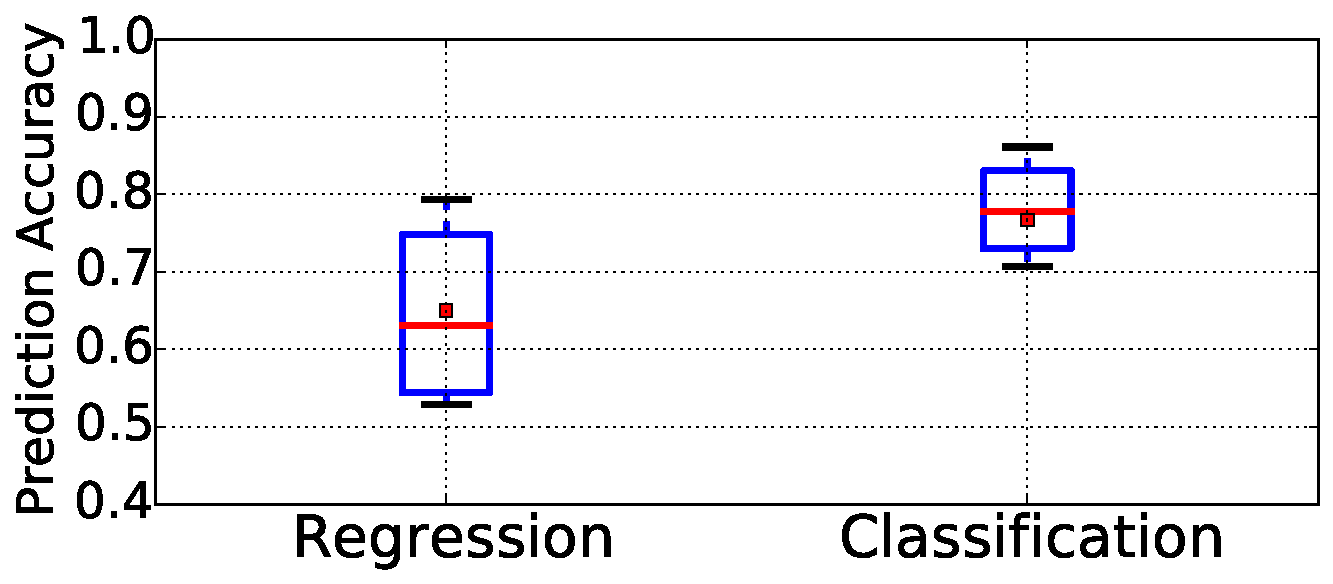
\includegraphics[width=.8\textwidth]{figures/multiple_prediction_accuracy.pdf}
 \centering
 \caption{\textbf{On the model selection of predicting the next step.}
 We evaluate the ability to distinguish a good and a bad configuration.
 In regression, we test rank preserving as prediction accuracy~\cite{nair2017}.}
 \label{fig:reg_clas}
\end{figure}


\subsection{Search Hints}
This section explains how to extract search hints using
probabilistic classification methods
~\cite{friedman2001elements,zadrozny2001obtaining,zadrozny2002transforming}.
A probabilistic classifier predicts probability distribution over
predicted classes.
In \myequation{\ref{eq:3}}, the learning task ranks the relative
performance measure of two architectural configurations.
We can map ranks to classes.
For example, the rank function $\sigma$ outputs \emph{class 1} if
$\frac{y_j}{y_i} < 1.1$. Otherwise, the output is \emph{class 0}.
A binary classifier is able to answer ``is $x_j$ better than $x_i$?''
A probabilistic classifier outputs higher probability for \emph{class 1} if
a specific workload performs better on $x_j$ than $x_i$.

We use an example to illustrate this process.
Consider a configuration space ($S=\{S_1, S_2, S_3, S_4\}$).
An CAT optimizer starts with $S_1$ and $y_1 = \phi(S_1) = 10$ (the current best).
Let us assume we have collected historical data for
training the probabilistic classifier.
The predicted probability distribution over ${S_1, S_2, S_3, S_4}$ 
is $[-, 0.8, 0.2, 0.2]$.
The probability vector $P_{i}$ represents
``how likely $S_j$ is a better choice than $S_i$.''
A higher value indicates $S_j$ is more likely
to perform better than $S_i$. 
In this example, $S_2$ is a better choice than the others.
When the actual performance measure is better $\phi(S_2) \leq \phi(S_1)$,
then CAT optimizer found a better solution than the current best.

The above example uses a binary classifier, and
\scout uses multiclass classification.
The intuition for using multiple classes is that some configurations
yield similar performance, and \scout should not consider little improvement.
For example, we can define the classes to be ``better,'' ``fair,'' and ``worse.''
\scout favors the configurations in the ``better'' class.
\scout uses a predefined discretization policy
(based on user-defined thresholds)  to convert probability to discrete classes.
%For example, $\frac{\phi(S_j)}{\phi(S_i)} \leq 0.8$ is considered as ``better.''
%\ick[do you mean i is better?]


\subsection{Search Strategy}

During the search process, a new observation
(running a workload on a selected cloud configuration)
provides the necessary information to determine
whether there exist better choices (see \myequation{\ref{eq:3}}).
The probability vector $P_{i}$ is derived
for each new observation $\phi(S_{i})$.
A search strategy determines the choice based on the probability predictions.
At each step, the search process selects the configuration $S_j$ with
the maximum probability in $P_{i}$.

This search strategy is similar to depth-first search.
While \emph{CherryPick} requires balancing exploration and exploitation,
\scout tends to exploit---because it uses historical data.
When the prediction model can generate quality predictions,
this search strategy leads to quick convergence speed
(the selected configuration improves over the current best).
Therefore, the search process has low search cost to find near-optimal
configurations. 

A search process should stop when it no longer can find a better configuration. This is controlled by a predefined parameter called  \textit{probability threshold} ($\alpha$) and acts as a stopping criterion.
When the predicted probability $P_{ij}$ is lower than $\alpha$ for all $S_j$,
the search process is not confident that it would find better configurations in the next step.
A search should also stop if it fails to find better solutions due to an inaccurate performance model. This is controlled by another parameter called \textit{ misprediction tolerance} ($\beta$) to avoid excessive search cost.

\subsection{Putting It All Together}
We have shown that the core element of a search based method is to determine
the next best step.
For obtaining hints to guide a search process,
we propose using the probabilistic classification technique
to predict improvement probability.
That is similar to Expected Improvement (EI) in \emph{CherryPick}.
We choose pairwise comparison and relative ordering
to deliver high prediction accuracy and to naturally into the search process.
\scout leverages low-level performance information and
extracts rules (based on resource utilization) implicitly.
This improves a search process because certain types of cloud configurations
can be avoided (as we will show in Section~\ref{sec:evaluation}).
Last, we choose a search strategy that merely picks the configuration
that is most likely to be better than the current best.
This strategy increases convergence speed---has low search cost.

\section{Implementation}
\label{sec:system}

This section describes the implementation of \scout
as shown in \myfigure{\ref{fig:system_design}}.
We implement the system in Python with
scikit-learn~\cite{scikit-learn} for machine learning libraries and
Boto 3~\cite{boto3} for interacting with Amazon web services.


\begin{figure}[!htbp]
 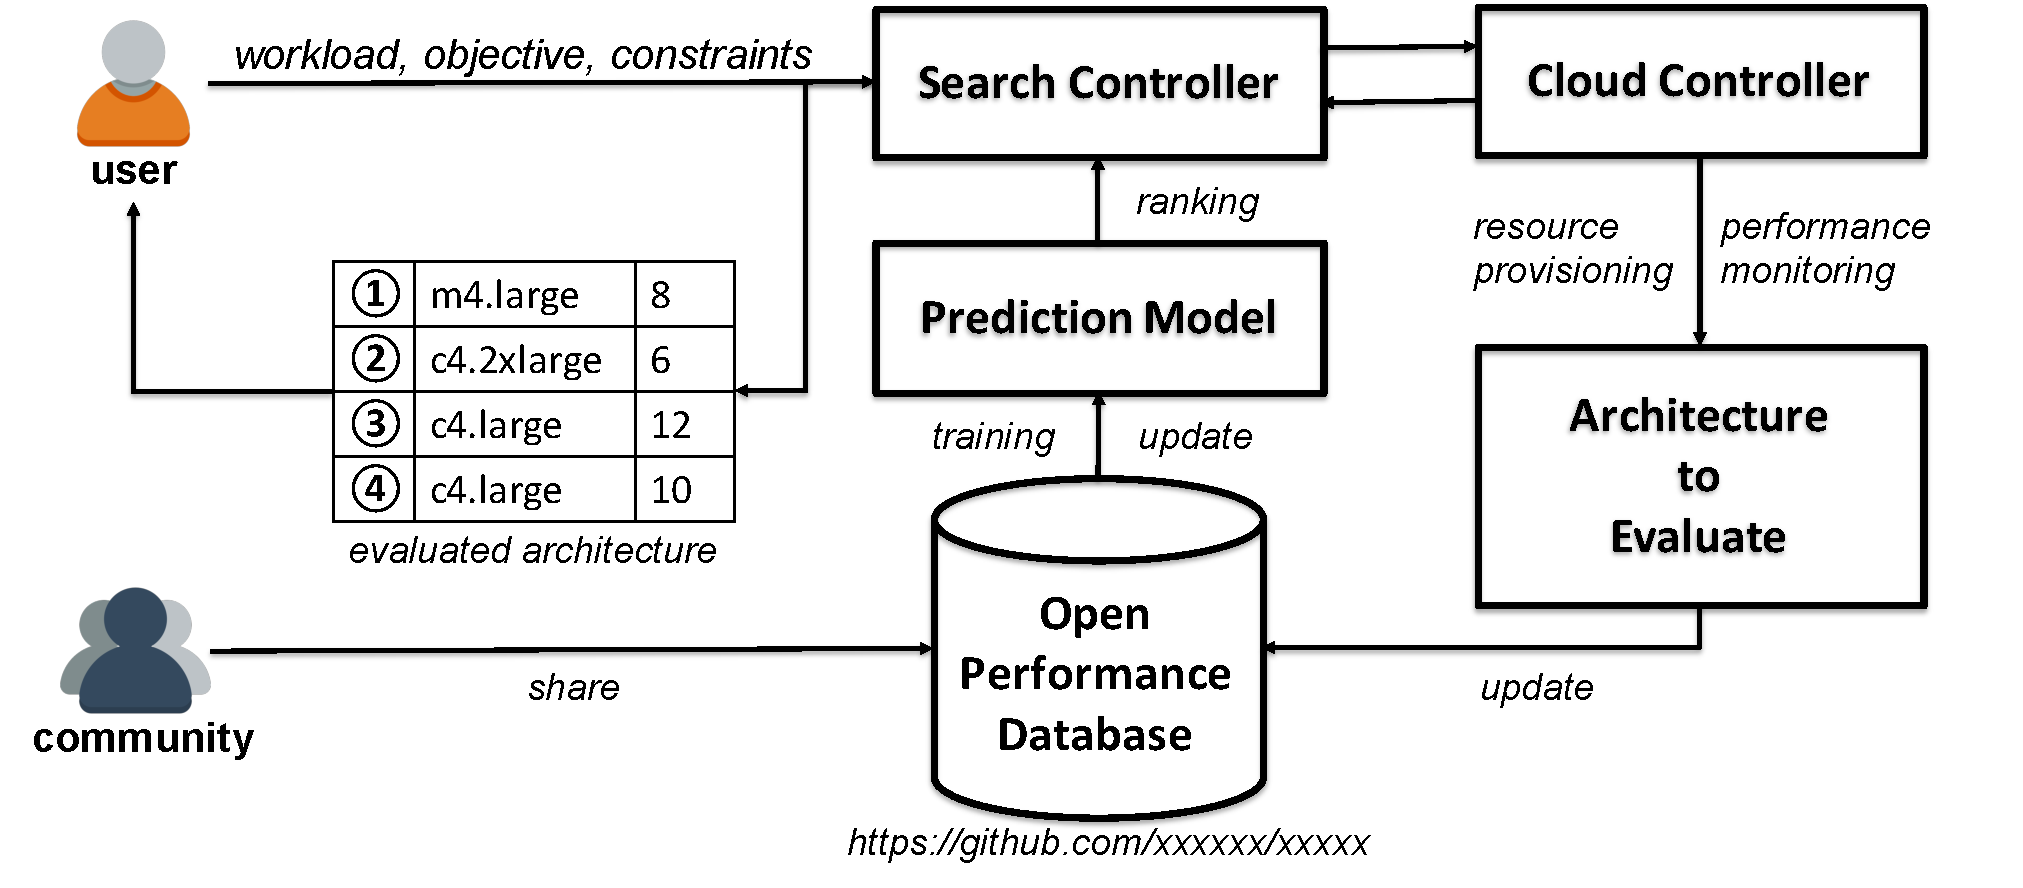
\includegraphics[width=.8\textwidth]{figures/system_design_blind.pdf}
 \centering
 \caption{\small{\textbf{\scout's implementation.}
 }}
 \label{fig:system_design}
\end{figure}


\begin{itemize}
\item \textbf{Search Controller.}
This is the entry point to use \scout.
A user submits a workload along with performance and cost objectives.
The user can also specify constraints such as maximum execution time,
maximum cost budget and the range of cluster sizes, etc.
The performance of \scout is not heavily affected by
the initial architectural configurations.
For evaluations, \scout randomly selects one configuration.
The search controller forwards the workload and the selected configuration
to the cloud controller.
Once the selected configuration is evaluated,
the search controller is notified and determines
the next configuration to evaluate.
\scout selects the configuration that, according to the model, has the
greatest likelihood of improving performance.
% The probability information is provided by the prediction model.
This optimization process stops when the objective is fulfilled or
when the evaluation budget is expended.

\item \textbf{Prediction Model.}
We can use a probabilistic classifier to derive the probability distribution
over prediction classes~\cite{friedman2001elements}.
Possible choices include, but are not limited to,
Logistic Regression, Gaussian Process, Random Forests and neural networks
~\cite{breiman2001random,friedman2001elements}.
\scout uses \emph{ExtraTree}
to train a classification model
for deriving relative ordering (to determine better configurations)
because \emph{ExtraTree} is more efficient and reliable
% to cope -- check this. does it still make your point?
with
numerical performance data~\cite{geurts2006extremely}.

\item \textbf{Cloud Controller.}
The cloud controller bridges the search controller and cloud platforms.
The controller is responsible for running the workload
with a specific architectural configuration.
\scout currently supports AWS but easily can be extended
to other cloud platforms.
For each evaluation, the cloud controller monitors the execution time and
collects low-level performance information.
We use the \emph{Sysstat} package on Linux for system monitoring~\cite{sysstat}.
Since we collect only generic performance metrics, other monitoring tools
should work as well.
We choose a five-second sampling period.
Each sample has 72 metrics from
CPU, memory, cache, disk and network components.
These numbers are then aggregated from various-size
samples (per node) and nodes (per cluster).
We follow the similar process of feature transformation
as described in~\cite{Hsu2016,Hsu2018Arrow}.

\item \textbf{Open Performance Database.}
Performance data is hard to find.
We believe sharing data can greatly advance the research
on CAT.
Moreover, cloud users benefit from the performance database because
they are able to learn the workload performance on
different architecture configurations, which are very expensive
to obtain.

\end{itemize}
\section{Evaluation}
\label{sec:evaluation}

We evaluate \scout with three sets of big data analytics
applications on 18 cloud configurations on a single-node.
We further evaluate 69 cloud configuration on multiple nodes.
Our evaluations show that \scout finds the optimal or near-optimal configuration more often than other methods
and does so while reducing search costs.

\subsection{Experiment Setup}
\label{sec:setup}

\subsubsection*{Workloads}
We choose diverse workloads (CPU-intensive, memory-heavy, IO-intensive and network-intensive) such as PageRank, sorting, recommendation, classification and online analytical processing (OLAP).
We also change the input parameters and data sizes to create
a wide spectrum of workloads. 
These workloads run on Apache Hadoop~\cite{hadoop} and two separate versions of Apache Spark~\cite{spark} (version 1.5 and 2.1). 

\begin{figure}[!htbp]
\centering
\begin{subfigure}[b]{0.4\textwidth}
    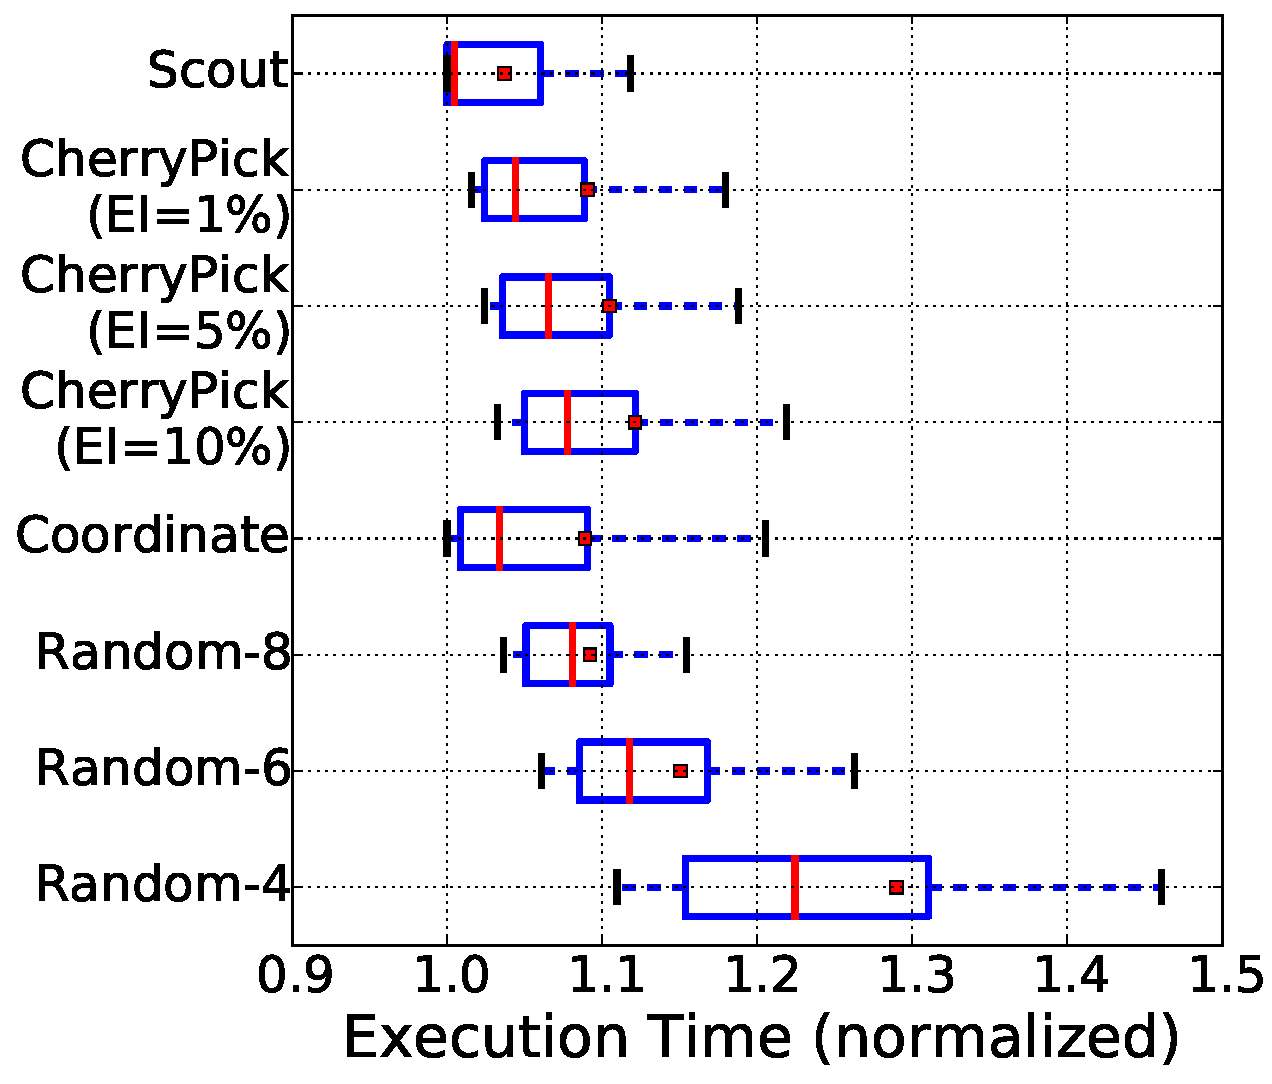
\includegraphics[width=\linewidth]{figures/single_time_overall_performance.pdf}
    \caption{Search Performance}
    \label{fig:single_time_overall_performance}
\end{subfigure}
\begin{subfigure}[b]{0.4\textwidth}
    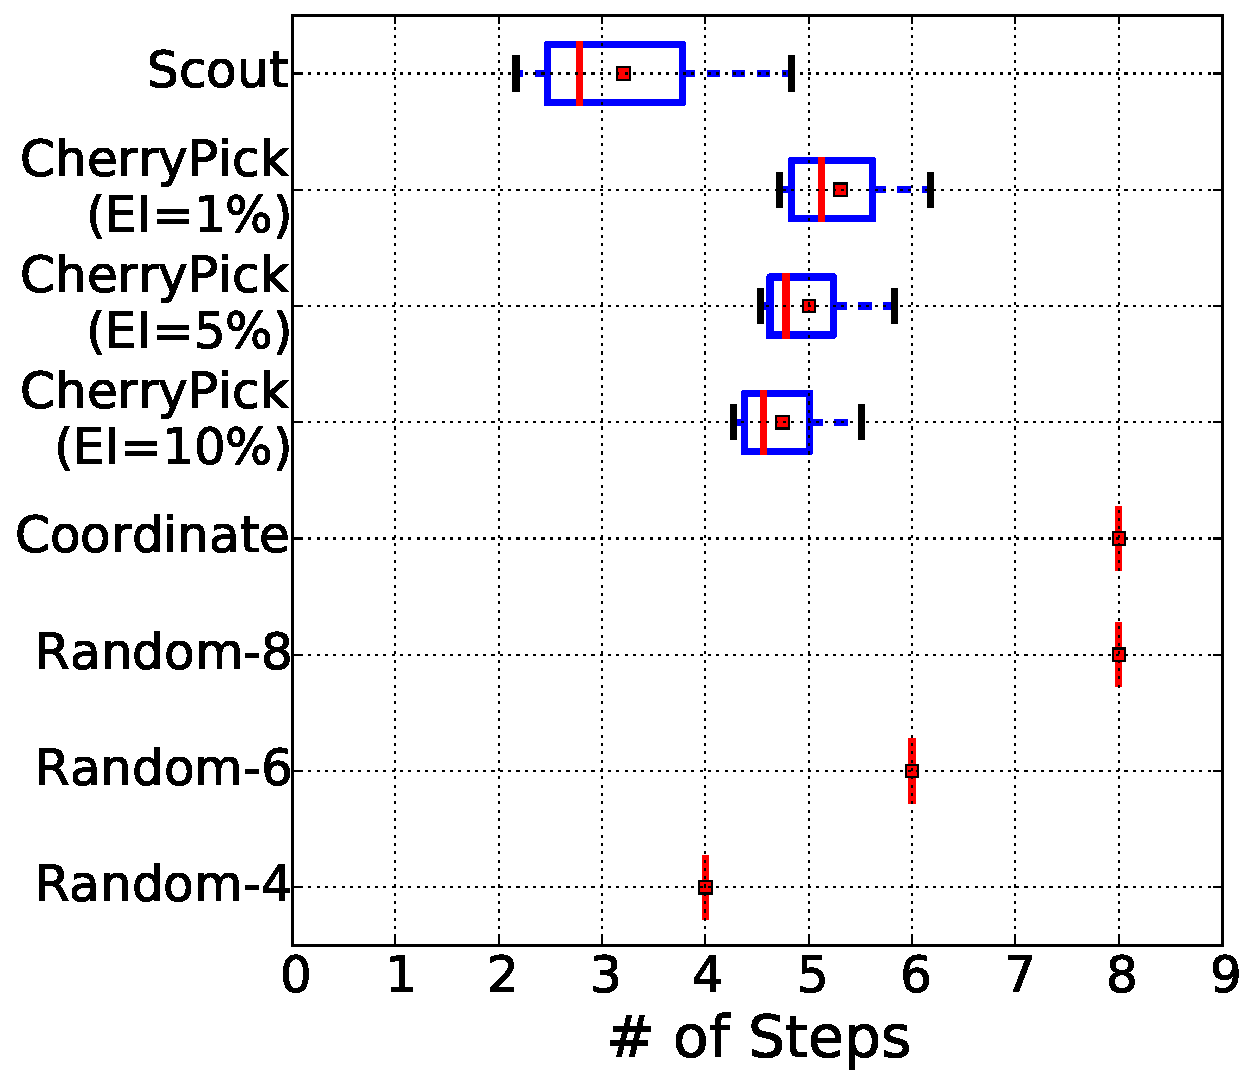
\includegraphics[width=\linewidth]{figures/single_time_overall_steps.pdf}
    \caption{Search Cost}
    \label{fig:single_time_overall_steps}
\end{subfigure}
\caption{\small{\textbf{Minimizing Execution Time.}
 The \emph{x-axis} represents the normalized performance (to the optimal configuration), and the optimal performance is $1$. 
 \scout finds the near-optimal solutions ($< 1.1$) in 87\% workloads while using much fewer steps.}}
\label{fig:single_time_overall}
\end{figure}


\subsubsection*{Deployment Choices}
Our evaluation examines both single- and multiple-node settings.
The single-node setting serves a comparison baseline and allows us to test more workloads (due to smaller search space).
In the single node setting,
we choose 18 distinct instance types or cloud configurations and 107 workloads.
When evaluating different cluster sizes,
we use strong scaling---fixed problem size---because we are interested in how to speed up a workload rather than the efficiency of the cluster.
For the multiple-node setting, we run 18 workloads
on 69 cloud configurations (9 instances with various cluster sizes).
%The search space is shown in~\myfigure{\ref{fig:search_space}}.

\subsubsection*{Dataset}
In order to verify the effectiveness of \scout,
we create a comprehensive performance data conversing all the combinations of
workloads and architectural configurations.
We collected our data on AWS.
\mytable{\ref{tab:dataset_overview}} present a summary.
Please refer to the open performance database for further details in Section~\ref{sec:cat::dataset}.


\subsubsection*{Parameters}
\scout has three important parameters:
1) labeled classes, 2) probability thresholds and 3) misprediction tolerance.
For the labeled classes in classification modeling,
we define five classes,
``better+'', ``better'',  ``fair'', ``worse'' and ``worse+'',
using thresholds [0.8, 0.95, 1.05, 1.2] as the cut points.
Regarding the two stopping criteria,
we choose $0.5$ for the probability threshold and
$3$ and $4$ for the misprediction tolerance
in the single-node and multiple-node setting respectively.
We examine the trade-off of these parameters in Section~\ref{sec:discussion}.

\subsection{Comparison Method}
To evaluate \scout, we examine the search performance
in terms of \emph{effectiveness}, \emph{efficiency} and \emph{reliability}.
We compare \scout with random search, coordinate descent, and \emph{CherryPick}.

\subsubsection*{Random search}
This search method
uniformly samples the configuration space.
The stopping criterion is the number of
configurations to evaluate.
A higher number yields better solution but also incurs higher search cost.
For a fair comparison, the search is repeated 100 times.  Random-4, -6, -8 represent random samples of 4, 6, and 8 cloud configurations respectively.
It serves as a na\"ive baseline method.


\begin{figure}[!htbp]
\centering
\begin{subfigure}[b]{0.4\textwidth}
    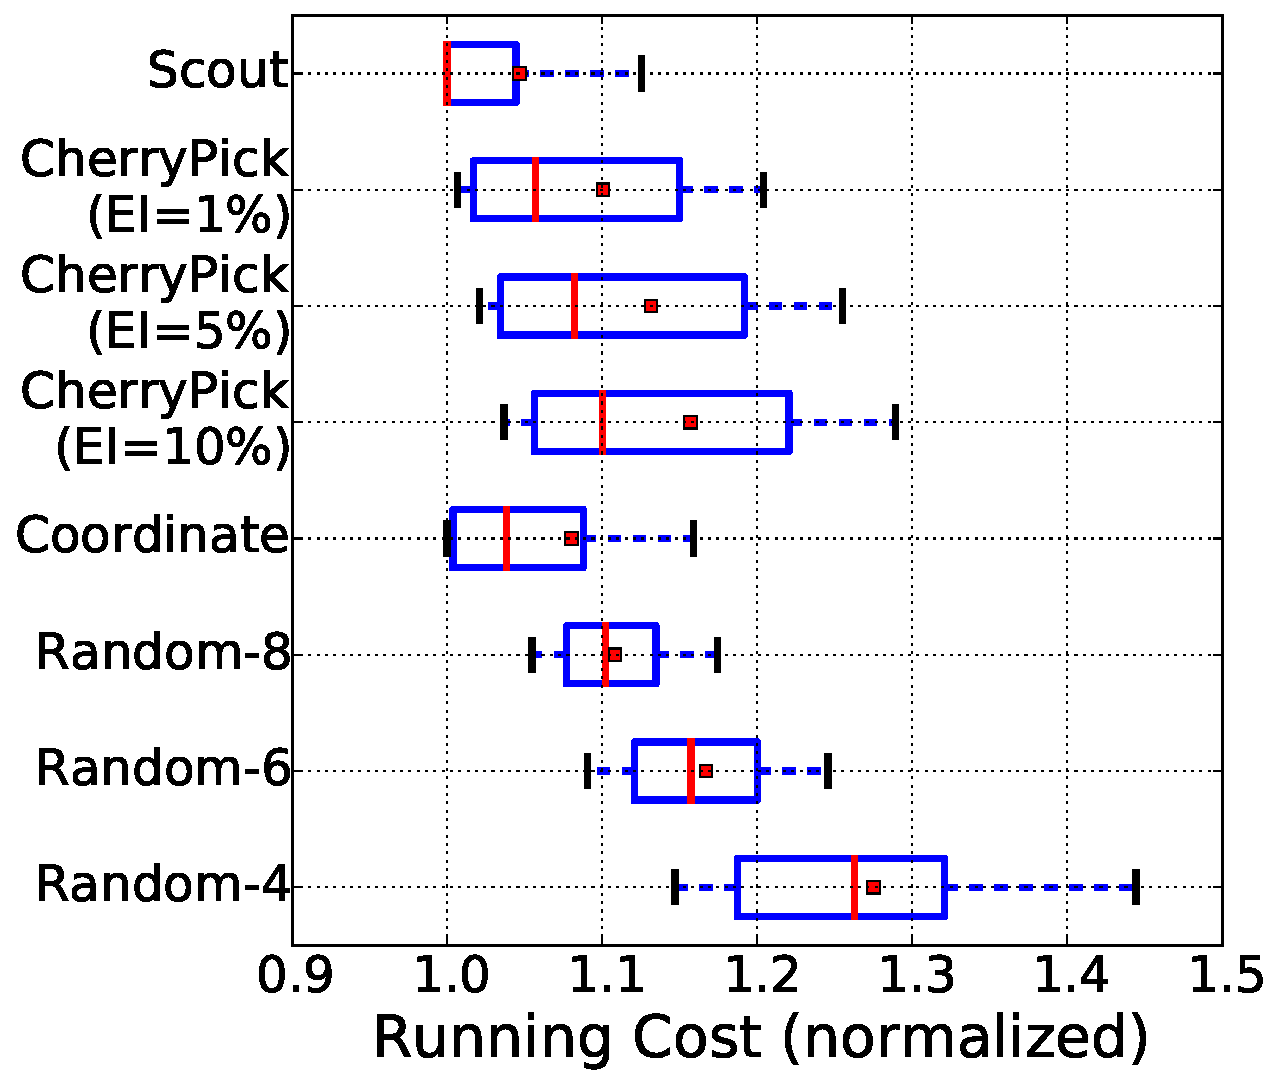
\includegraphics[width=\linewidth]{figures/single_cost_overall_performance.pdf}
    \caption{Search Performance}
    \label{fig:single_cost_overall_performance}
\end{subfigure}
\begin{subfigure}[b]{0.4\textwidth}
    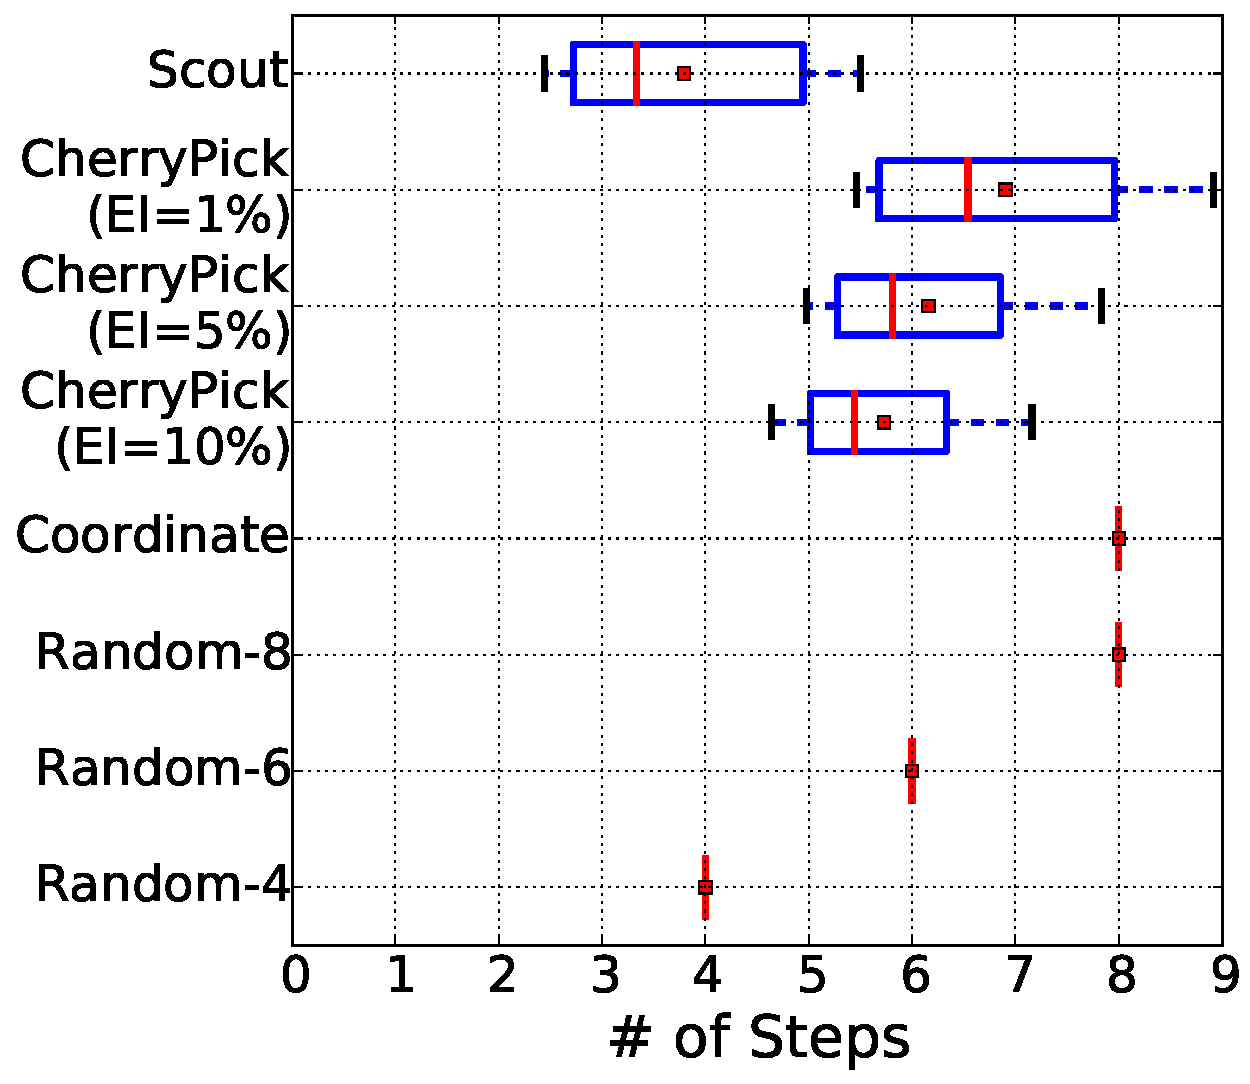
\includegraphics[width=\linewidth]{figures/single_cost_overall_steps.pdf}
    \caption{Search Cost}
    \label{fig:single_cost_overall_steps}
\end{subfigure}
\caption{\small{\textbf{Minimizing Running Cost.}
 Searching for the optimal cost is more difficult because the search cost is higher than the scenario of minimizing execution time. \scout still finds near-optimal solutions with a small increase in search cost while \emph{CherryPick} only finds near-optimal solutions in about 50\% workloads.}}
\label{fig:single_cost_overall}
\end{figure}


\subsubsection*{Coordinate descent}
This method searches
one dimension (\eg{CPU type and memory size}) at a time.
It determines the best choice of the dimension and
continues to choose the best from other dimensions.
This approach may suffer from local minimum due to
diminishing return and irregular performance outcome~\cite{Alipourfard2017}.
This situation worsens when the number of dimension increases.
In the evaluation, there are three dimensions:
(1) the instance family (such as \emph{c4} or \emph{r4}), (2)
the instance size (such as, \emph{large} or \emph{2xlarge}), and (3) the cluster size (the number of VMs).
The results are from 100 distinct searches, in which the starting point was randomly selected.


\subsubsection*{\cherrypick}
We implement the approach
proposed in \emph{CherryPick}~\cite{Alipourfard2017}.
We use
the same kernel function (\emph{Mat\'ern 5/2}) and
the same stopping criteria (\textbf{EI}=10\%).
We uniformly sample three configurations as starting points.
Since the search performance of \emph{CherryPick} is highly dependent on the selection of the starting points,
this experiment repeats 100 times to reduce artifacts
and give a better picture of \emph{CherryPick}'s capability.

We compare these approaches using three metrics.
First, we evaluate the effectiveness of the methods using
the \textit{normalized performance} (to the optimal choice).
It can be the \textit{execution time} or the \emph{deployment cost}.
Second, we use the search cost--- the number of cloud configurations measured to find the right cloud configuration.
% We consider the number of steps instead of the search cost (the total cost of actual measurements) because the former reveals how fast a method finds a solution.
Last, we examine how reliable our method is across the workloads. % (in single node setting) and 18 (in multiple-node setting).
We compare the aggregate of the normalized performance and the search cost along with their the 10\textsuperscript{th} and 90\textsuperscript{th} percentiles to observe whether our method performs well with consistency.  These numbers better illustrate reliability of the methods.


\begin{figure}[!htbp]
\centering
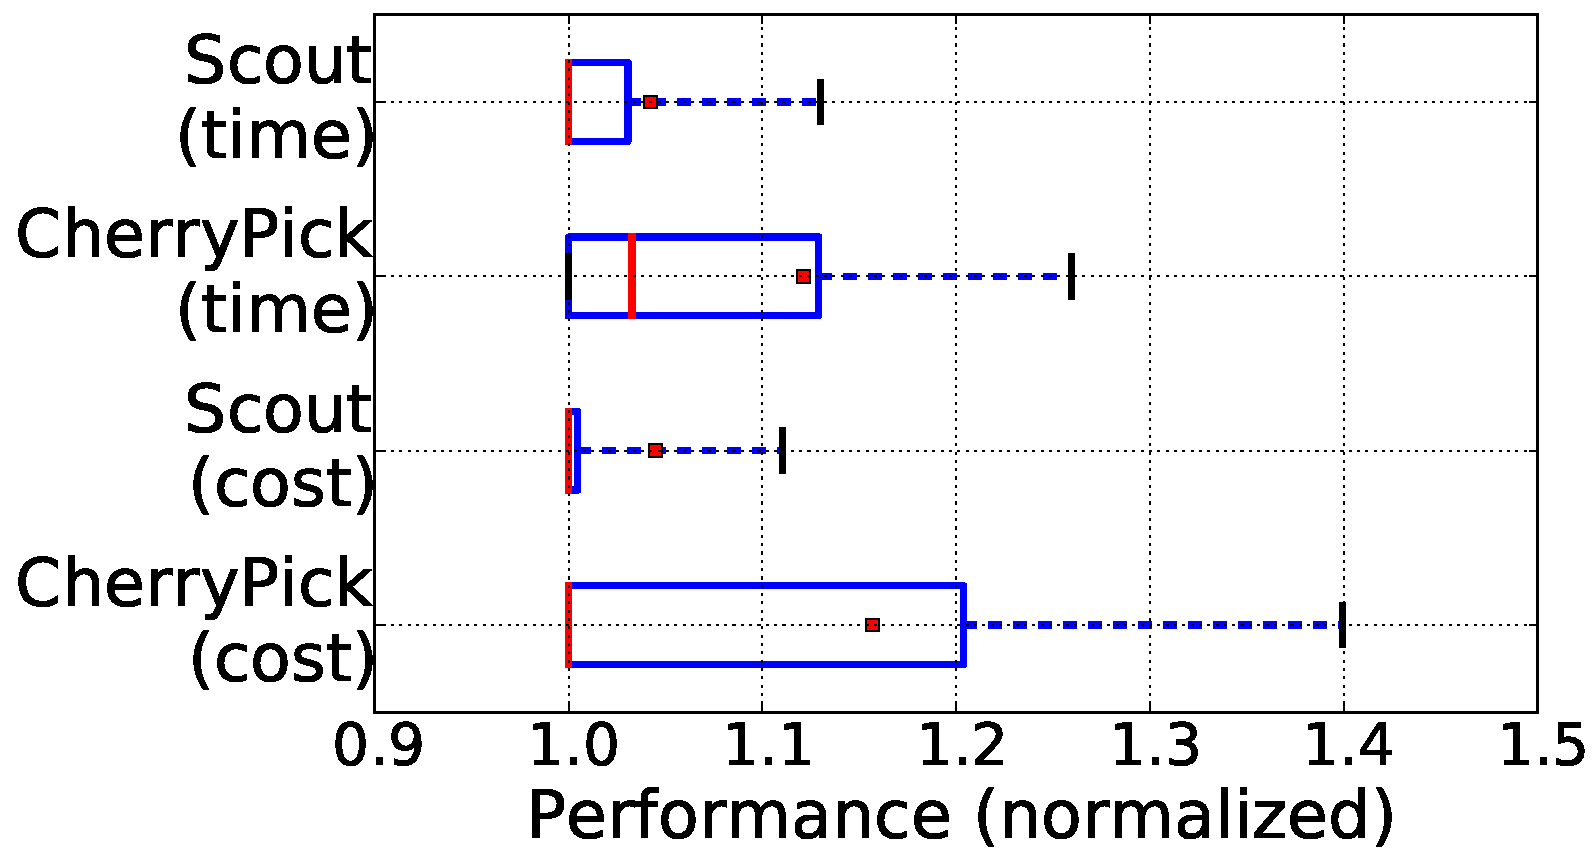
\includegraphics[width=0.6\textwidth]{figures/single_fragility.pdf}
\caption{\small{\textbf{Quality of found solutions.}
    Although both \emph{CherryPick} and \scout find the near optimal-solutions in most of the time,
    \scout is less fragile.}
}
\label{fig:single_fragility}
\end{figure}

\begin{figure}
\centering
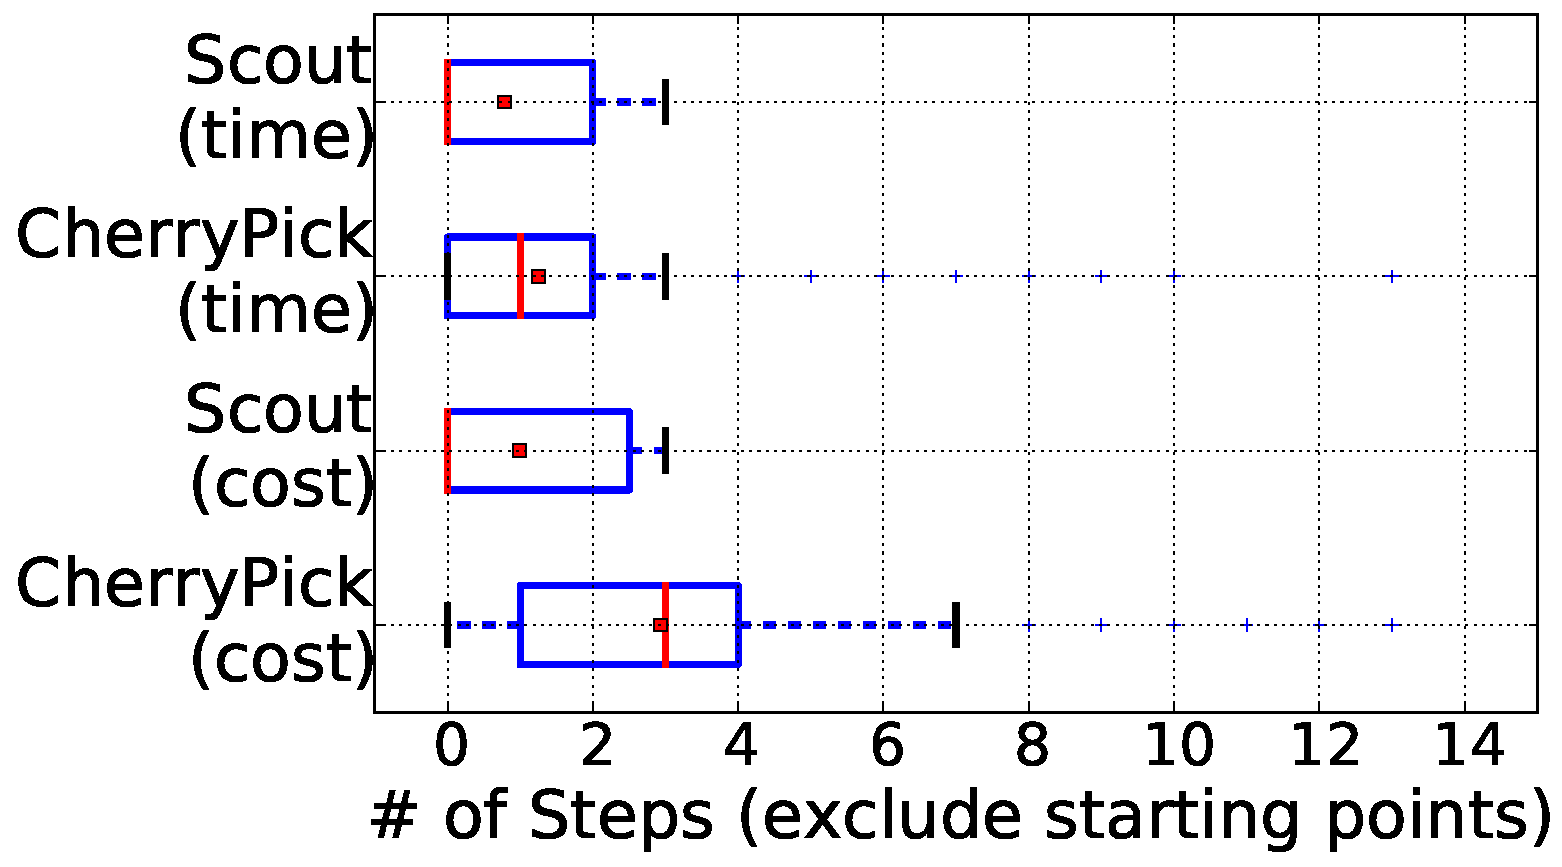
\includegraphics[width=0.6\textwidth]{figures/single_stopping_awareness.pdf}
\caption{\small{\textbf{Stopping awareness.}
    Search optimization avoids unnecessary search cost if it knows when the optimal solution is found.
    % \scout better acknowledges its existence.
    }}
\label{fig:single_startingpoint}

\end{figure}

\begin{figure}
\centering
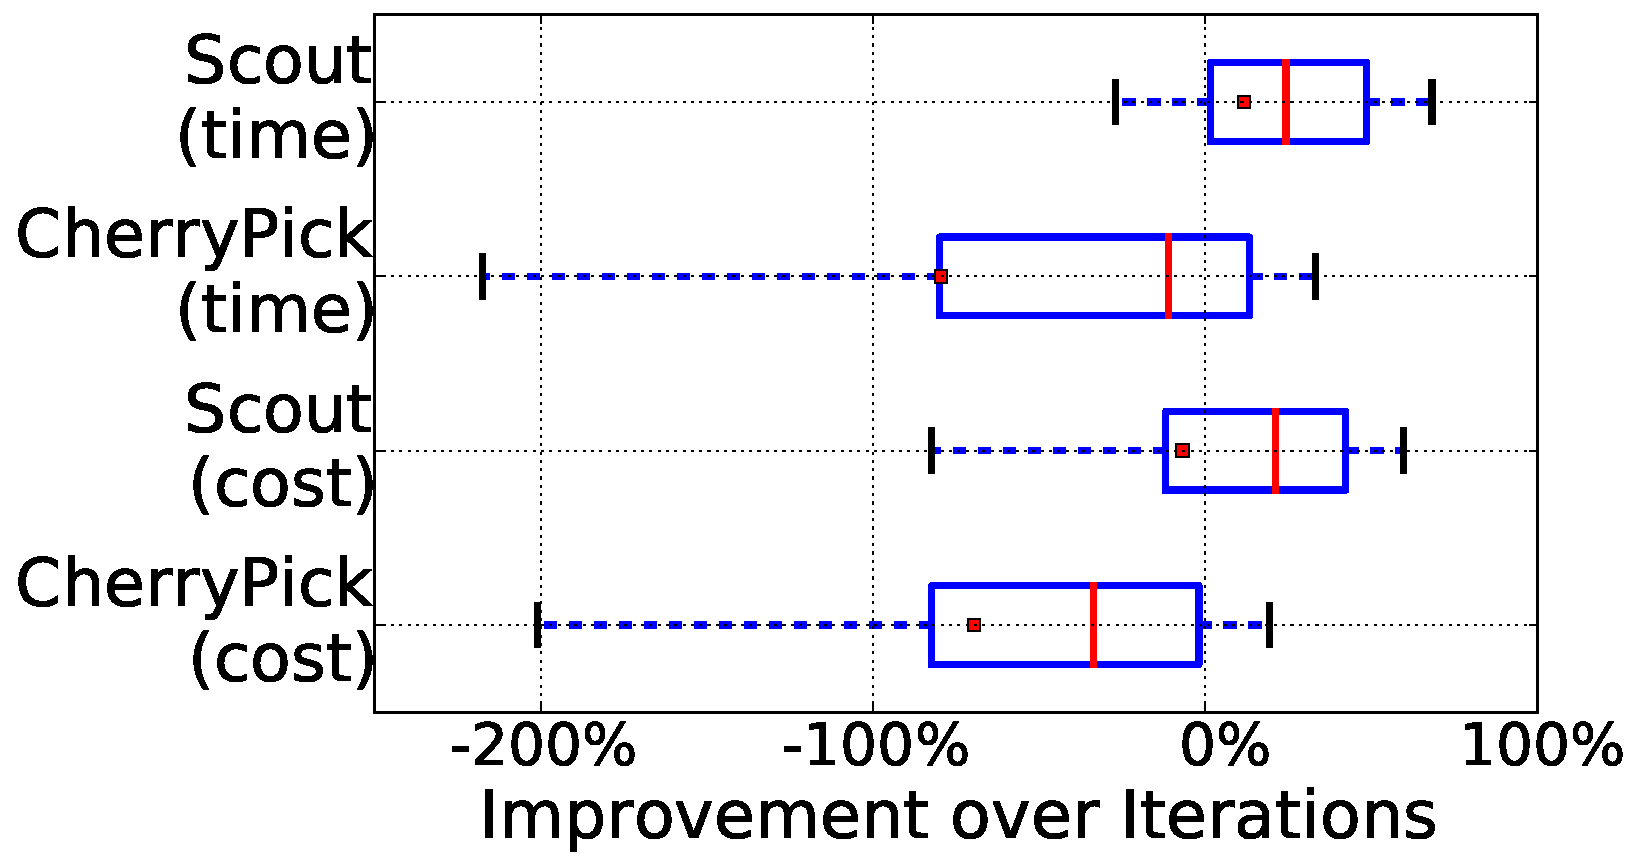
\includegraphics[width=0.6\textwidth]{figures/single_convergence.pdf}
\caption{\small{\textbf{Convergence speed.}
    \scout finds a better solution with 25\% improvement (on average) at each iteration, which suggests \scout is more likely to 
    converge.}}
\label{fig:search_convergence}
\end{figure}


\subsection{Is Scout effective and efficient?}

We examine search performance and search cost across 107 workloads in the single-node setting.
This evaluation largely answers whether a search method is reliable.

\textbf{Scout finds the near-optimal configurations
(within 10\% difference) for 87\% workloads}.
\myfigure{\ref{fig:single_time_overall_performance}} and \myfigure{\ref{fig:single_cost_overall_performance}} presents
the best cloud configuration (normalized to the optimal performance---1.0 represent the best, higher the worse) found by \scout and other methods while minimizing execution time and deployment cost, respectively. \myfigure{\ref{fig:single_time_overall_steps}} and \myfigure{\ref{fig:single_cost_overall_steps}} presents the search cost required the find the best cloud configuration which minimizes execution time and deployment cost, respectively. 
The figures display a box plot.
The box shows the inter-quartile range (from 25\textsuperscript{th} to 75\textsuperscript{th} percentile).
The vertical red line is the median, and the dot is the mean.
The whiskers to left and right show the 10\textsuperscript{th} and 90\textsuperscript{th} percentiles, respectively.
The horizontal axis shows execution time, and the vertical axis shows different techniques. 
An ideal search-based technique would find the best cloud configuration (in terms of performance) using the lower search cost.
These figures show the following.

\begin{itemize}[leftmargin=*]
    %\setlength\itemsep{-0.4em}
    \item \scout finds the best relative performance in terms of both execution time and deployment cost. The median performance of \scout, while searching for the cloud configuration which minimizes the deployment cost is 1.0, which means \scout was able to find the right cloud configuration.
    \item \scout is better than CherryPick across all measures (execution time, deployment cost, and search cost).
    \item \scout finds the best relative performance using the least search cost (fewer number of steps). Random-4 also requires low search cost, but its performance is much worse than \scout.
    \item The variance in the performance (in terms of execution time and deployment cost) of \scout is much lower than the other methods. The large variance of the Random methods can be attributed to their inherent randomness.
\end{itemize}


Overall, we see that \scout is that best performing method and \emph{CherryPick}, the state of the art method, only delivers similar performance in 64\% workloads while requiring 47\% greater search cost (4.7 compared to 3.2 steps). We also observe that the variance in the best cloud configuration found by \scout over 100 runs across 107 workloads is much lower than the other method. Hence, we can conclude that \scout is a reliable method to find the best cloud configuration.

\noindent\textbf{Cost creates a level playing field.}
Optimizing execution time is relatively easy
because a larger, more powerful instance type is more likely to have a shorter execution time.
However, the more powerful types are more expensive to execute.
Consequently, a smaller instance type may run longer but cost less.
Because the cost to execute an instance grow as the raw hardware performance increase, the differences in deployment cost between configurations tend to be much less than the differences between execution time.
This levels the playing field for cost---many more configurations are good candidates.
This leveling leads to, in general, longer searches,
as shown in \myfigure{\ref{fig:single_cost_overall_steps}}.
\emph{CherryPick} requires one extra step in optimizing deployment cost with a 15\% decrease of workloads in which it fails to find a solution within 10\% of the optimal configuration. To summarize, the performance of a search-based method is dependent on the objective of the search. From the data, we observe that searching for the best cloud configuration in terms of cost is more challenging than finding the best cloud configurations in terms of execution time. 




\subsection{Is \scout reliable?}
Users are willing to use a tool only when it is reliable. We evaluate the performance of \emph{CherryPick} and \scout
with different initial points for understanding their consistency.
In BO in \emph{CherryPick}, uses a random initial points to seed the search process and the effectiveness of CherryPick depend on these initial points. Selecting these initial points is non-trivial because (1) a good set of starting points for one workload does not work for other workloads, and (2) cloud providers frequently upgrade their instance portfolio with new instance types which make the process of selecting initial points more challenging. \scout is robust such that the effectiveness of \scout does not rely on initial points.


\begin{figure}[!htbp]
\centering
\begin{subfigure}[b]{0.4\textwidth}
    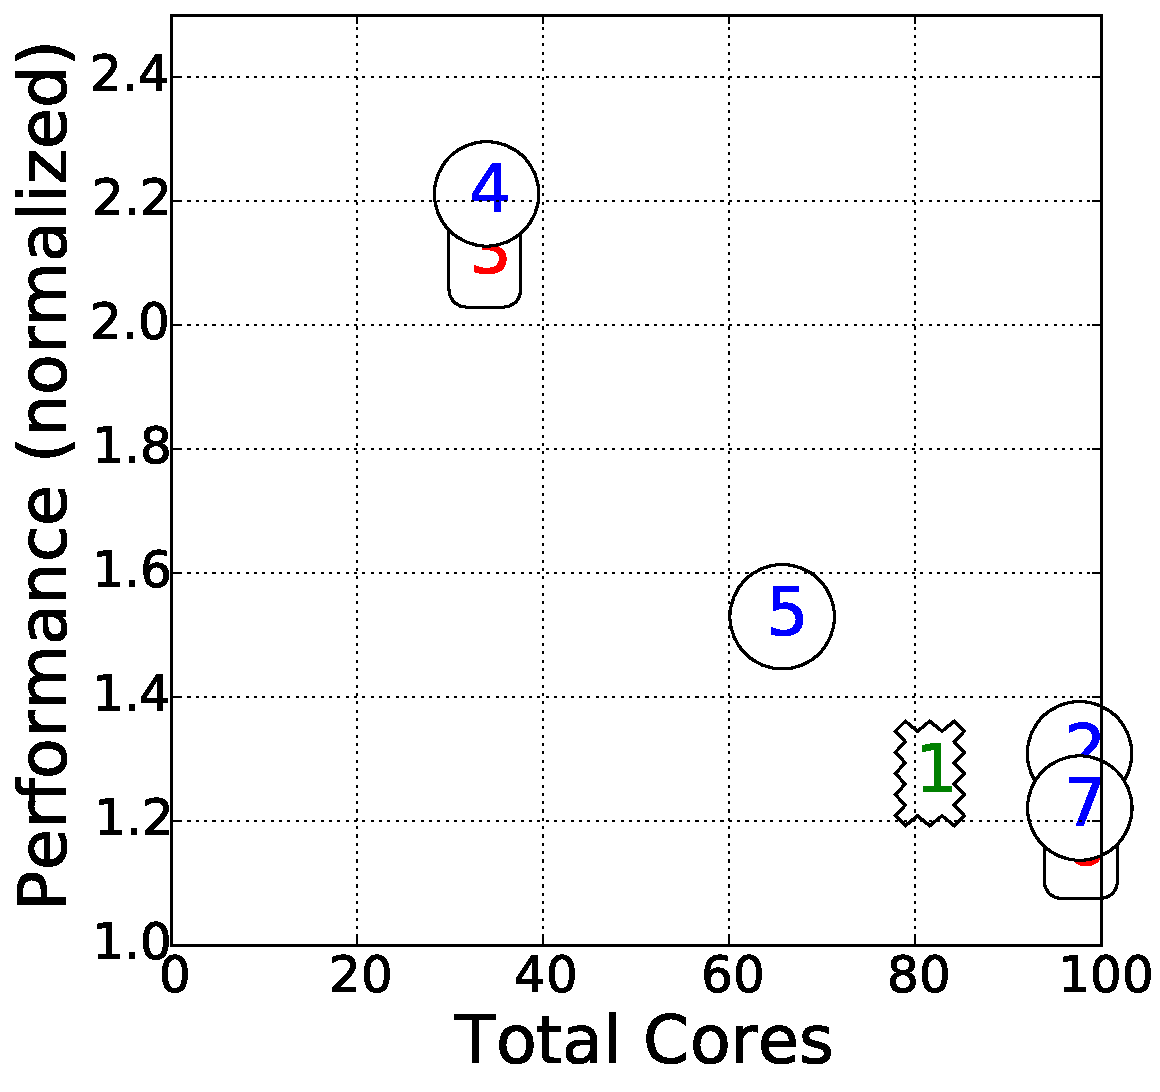
\includegraphics[width=\linewidth]{figures/multiple_bo_time_hadoop.pagerank.bigdata_12_cores.pdf}
    \caption{\cherrypick}
    \label{fig:comparison_time_cherrypick}
\end{subfigure}
\begin{subfigure}[b]{0.4\textwidth}
    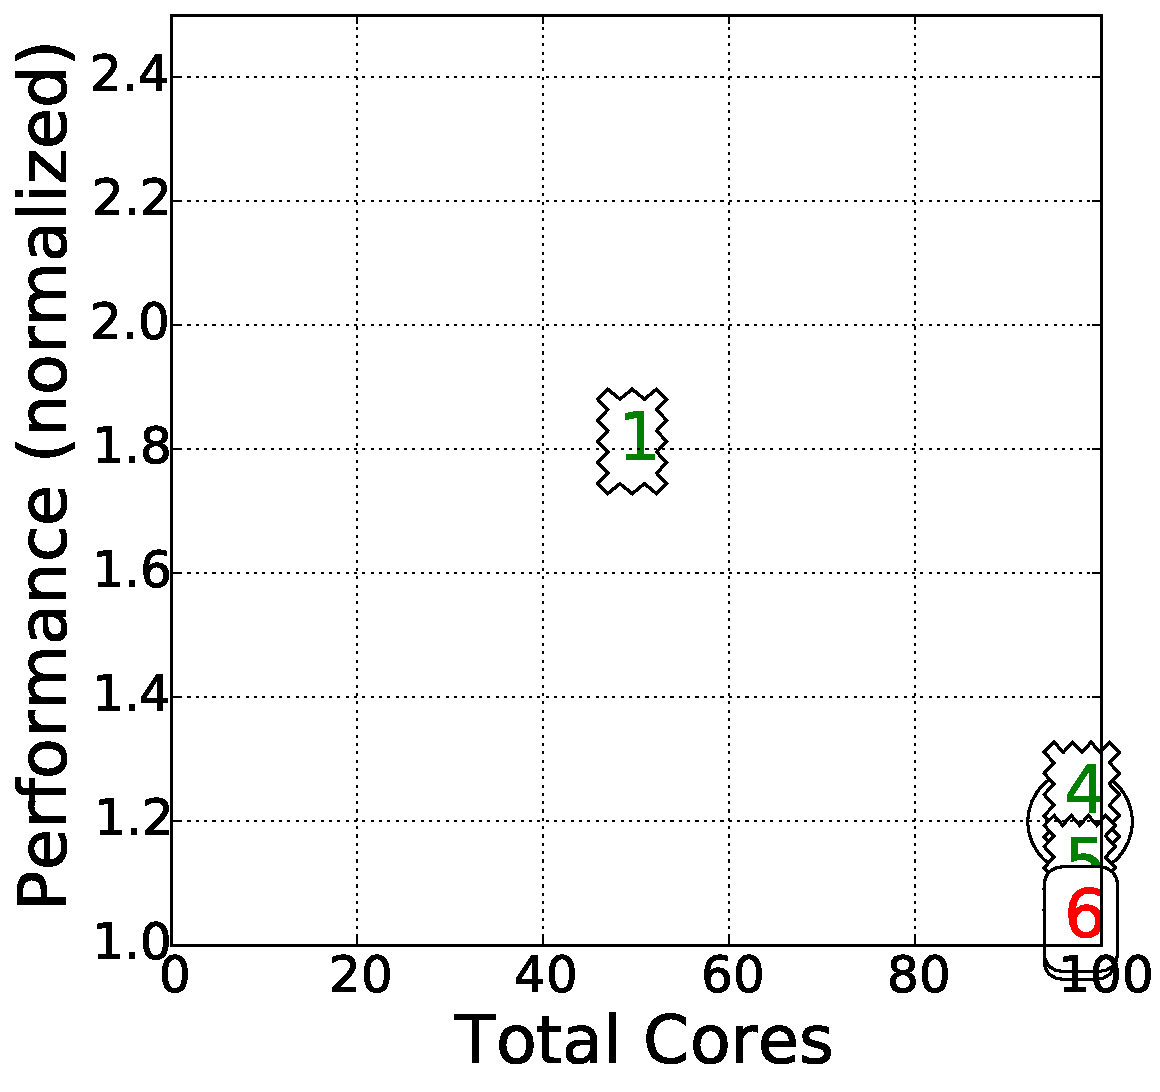
\includegraphics[width=\linewidth]{figures/multiple_scout_time_hadoop.pagerank.bigdata_24_m4.large_cores.pdf}
    \caption{\scout}
    \label{fig:comparison_time_scout}
\end{subfigure}
 \caption{\small{\textbf{Finding the fastest configuration for PageRank on Hadoop.} Left \& right sub-figure show the search path of CherryPick and \scout respectively. \scout identifies PageRank as a compute-intensive workload.  It chooses the configurations with higher core counts and CPU speed.}}
\label{fig:compare_1}
\end{figure}


To demonstrate the robustness of \scout, for each workload, we varied the initial points used in \emph{CherryPick}.
These points were randomly (without replacement) selected from the search space. On the other hand, \scout only needs one starting point, which is also selected randomly. This experiment was repeated 100 times to understand the implication of randomness.
\myfigure{\ref{fig:single_fragility}} shows the variance in the normalized performance of the found solutions by both the methods.
We see that 

\begin{itemize}[leftmargin=*]
    %\setlength\itemsep{-0.4em}
    \item \scout can find the optimal cloud configuration for most of the case since median performance is 1.0. However, there are some outliers which pushes the mean to 1.05. This is not a major concern since the 75$^{th}$ percentile is less than 1.05. This goes to show that the variance in the performance of 107 workloads aggregated over 100 runs is low.
    \item CherryPick is also effective in finding the cloud configuration since its median performance over 107 workloads is 1.05. We notice that the variance of the performance (both in terms of search performance and time) is larger than \scout. 
\end{itemize}


The variance in the results of CherryPick can be a major concern for the practitioners since a bad choice of initial points can lead to selecting either a slow or expensive configurations.
\scout, on the other hand, has more stable search performance regardless of the starting point.


\subsection{Why \scout works better?}
\label{sec:why_better}

\scout relies on quality routing policy to deliver good solutions.
We find \scout effective because
it knows when to stop searching and
converges to better solutions.

\begin{itemize}
\item \textbf{\scout knows when to stop.}
When an optimizer can stop as soon as it finds the optimal solution (or near-optimal solutions),
it can avoid unnecessary search efforts. \myfigure{\ref{fig:single_startingpoint}} shows that \scout requires a fewer number of steps if the starting point is already the optimal configuration.

\item \textbf{Convergence speed.}
The speed of convergence of a search-based method is dependent how it selects the next cloud configuration to measure. An ideal search-based method will always find the next cloud configuration, which is better than the cloud configurations sampled previously. \textit{Converge speed} can be defined as the average difference between the performance score (execution time or deployment cost) of the previous measurement (i$^{th}$ step) and the current measurement (i+1$^th$ step). A positive number would indicate that the current cloud configuration is better than the previous measurement (for both deployment cost and execution time, lower is better). \myfigure{\ref{fig:search_convergence}} compares the convergence speed of CherryPick and \scout. \myfigure{\ref{fig:search_convergence}} indicates that \scout overall finds cloud configurations 50\% (median) better execution time than the current cloud configuration, whereas CherryPick overall moves to cloud configuration which is 25\% worse than the current best configuration. Similar behavior is seen for deployment cost. This is evidence to show that \scout uses the historical data to find the promising region in the search space and exploits that space effectively.

\end{itemize}



\begin{figure}[!htbp]
\centering
\begin{subfigure}[b]{0.4\textwidth}
    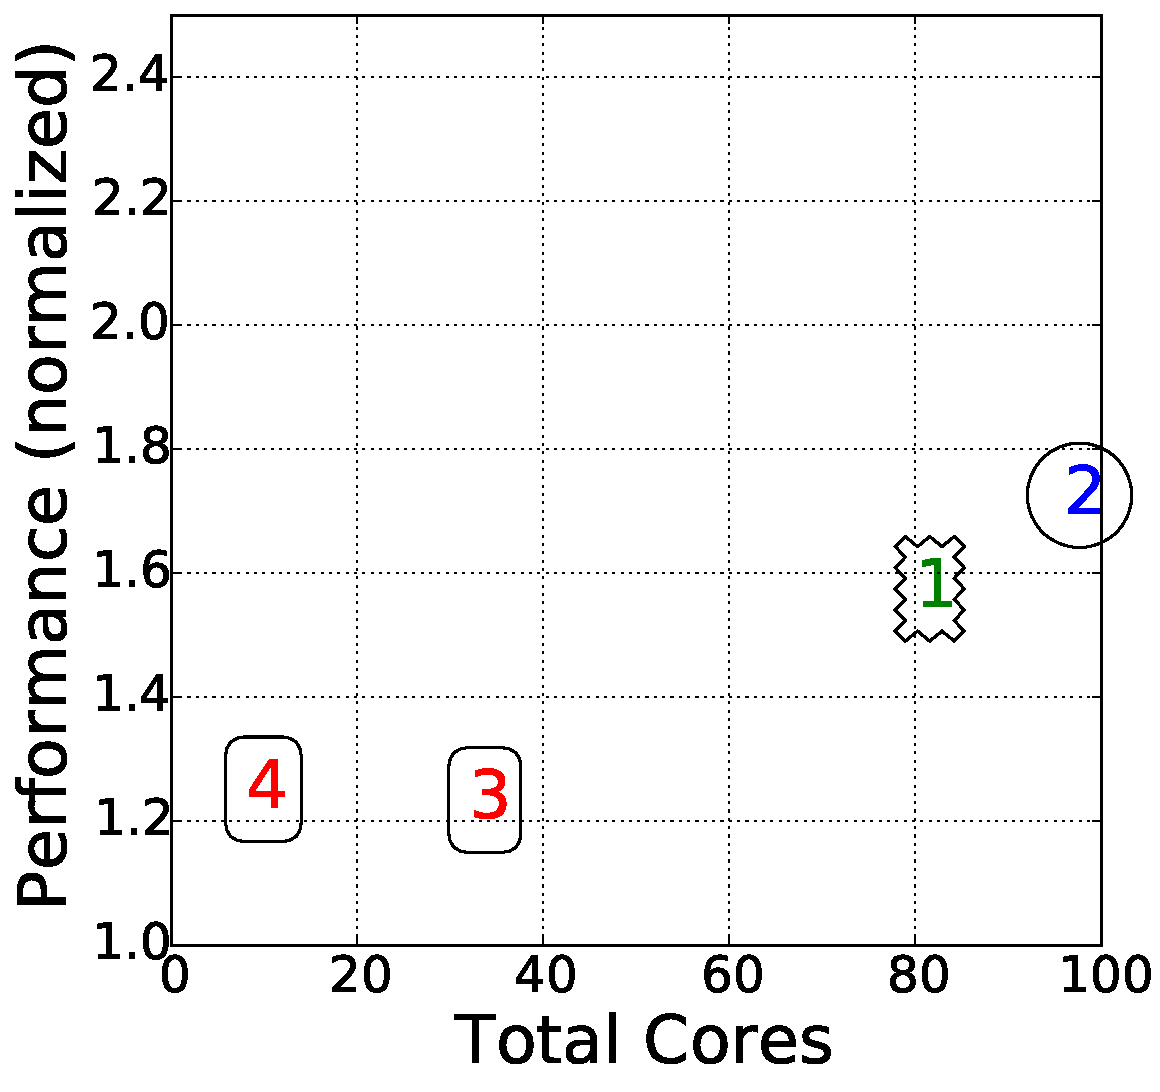
\includegraphics[width=\linewidth]{figures/multiple_bo_cost_spark1.5.naive-bayes.huge_12_cores.pdf}
    \caption{\cherrypick}
    \label{fig:comparison_cost_cherrypick}
\end{subfigure}
\begin{subfigure}[b]{0.4\textwidth}
    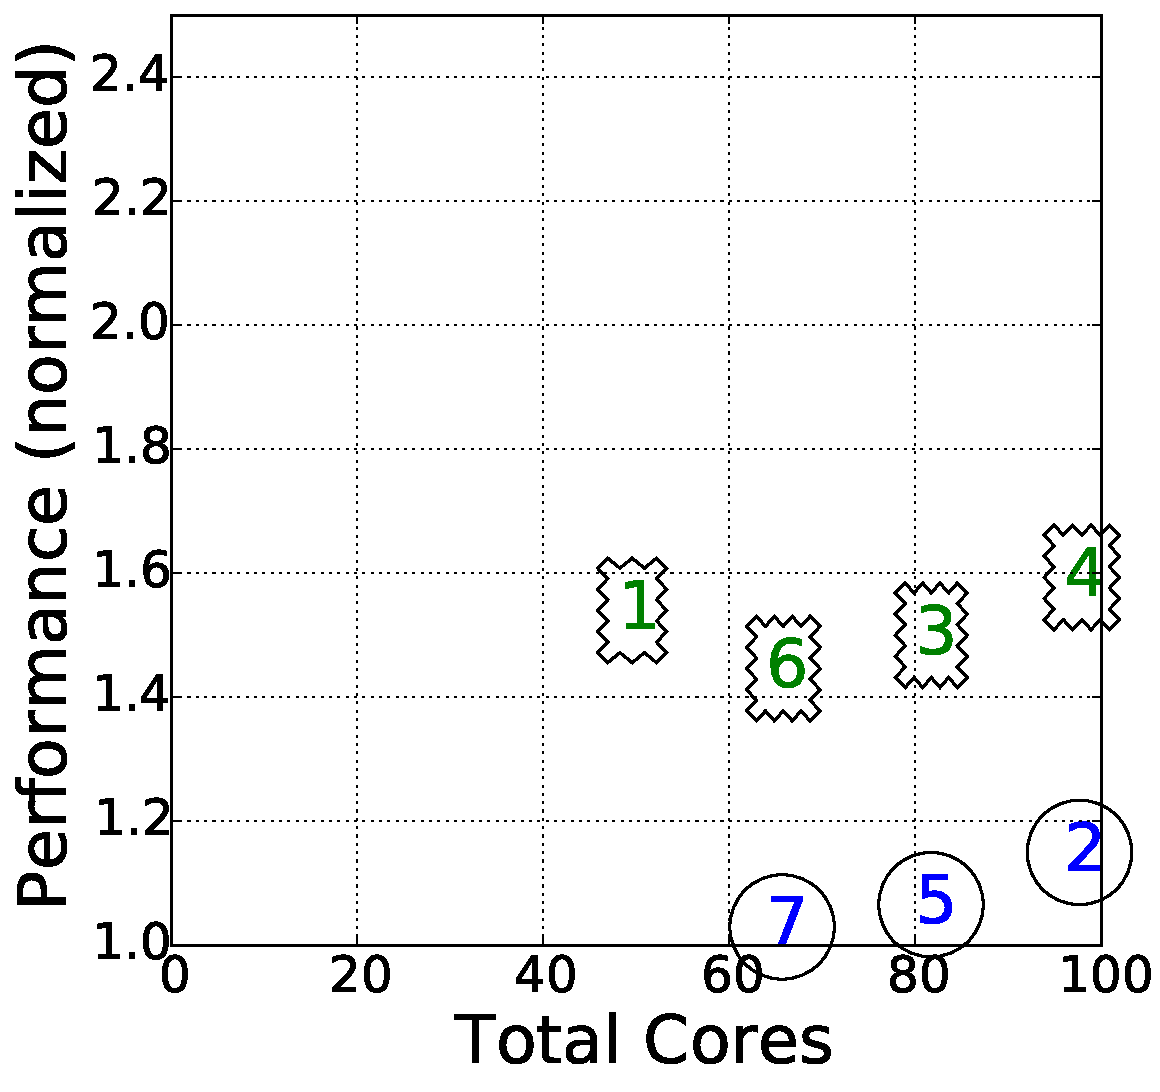
\includegraphics[width=\linewidth]{figures/multiple_scout_cost_spark1.5.naive-bayes.huge_24_m4.large_cores.pdf}
    \caption{\scout}
    \label{fig:comparison_cost_scout}
\end{subfigure}
\caption{\small{\textbf{Minimizing the running cost for Naive-Bayes on Spark.} This is a memory-intensive workload.  \scout does not even try the \emph{c4} family due to its small memory per core.}}
\label{fig:compare_4}
\end{figure}



\subsection{Example Search Process}

This section compares and contrasts the properties of \emph{CherryPick} and \scout.
We provides four examples of optimizing execution time (in Figure~\ref{fig:compare_1} and~\ref{fig:compare_2}) and running cost (in Figure~\ref{fig:compare_3} and~\ref{fig:compare_1}). Different colored markers in the graphs represent different families of instances: \textcolor{green}{green} represent the m4 family---general purpose, \textcolor{blue}{blue} represent the r4 family---memory optimized, and \textcolor{red}{red} represent the c4 family---compute optimized.
We evaluate \emph{CherryPick} and \scout on four representative workloads, selected based on diverse resource requirements (CPU intensive, Memory intensive).
For \emph{CherryPick}, we choose
\emph{20$\times$m4.xlarge}, \emph{48$\times$r4.large} and \emph{16$\times$c4.large} as the starting points because
they are wide spread in the search space.
Since \scout only needs one starting point,
we choose \emph{24$\times$m4.large} because it is the mid point of the search space.
We observe that \emph{CherryPick} can find near-optimal solutions for few workloads if not all.

\begin{figure}[!htbp]
\centering
\begin{subfigure}[b]{0.4\textwidth}
    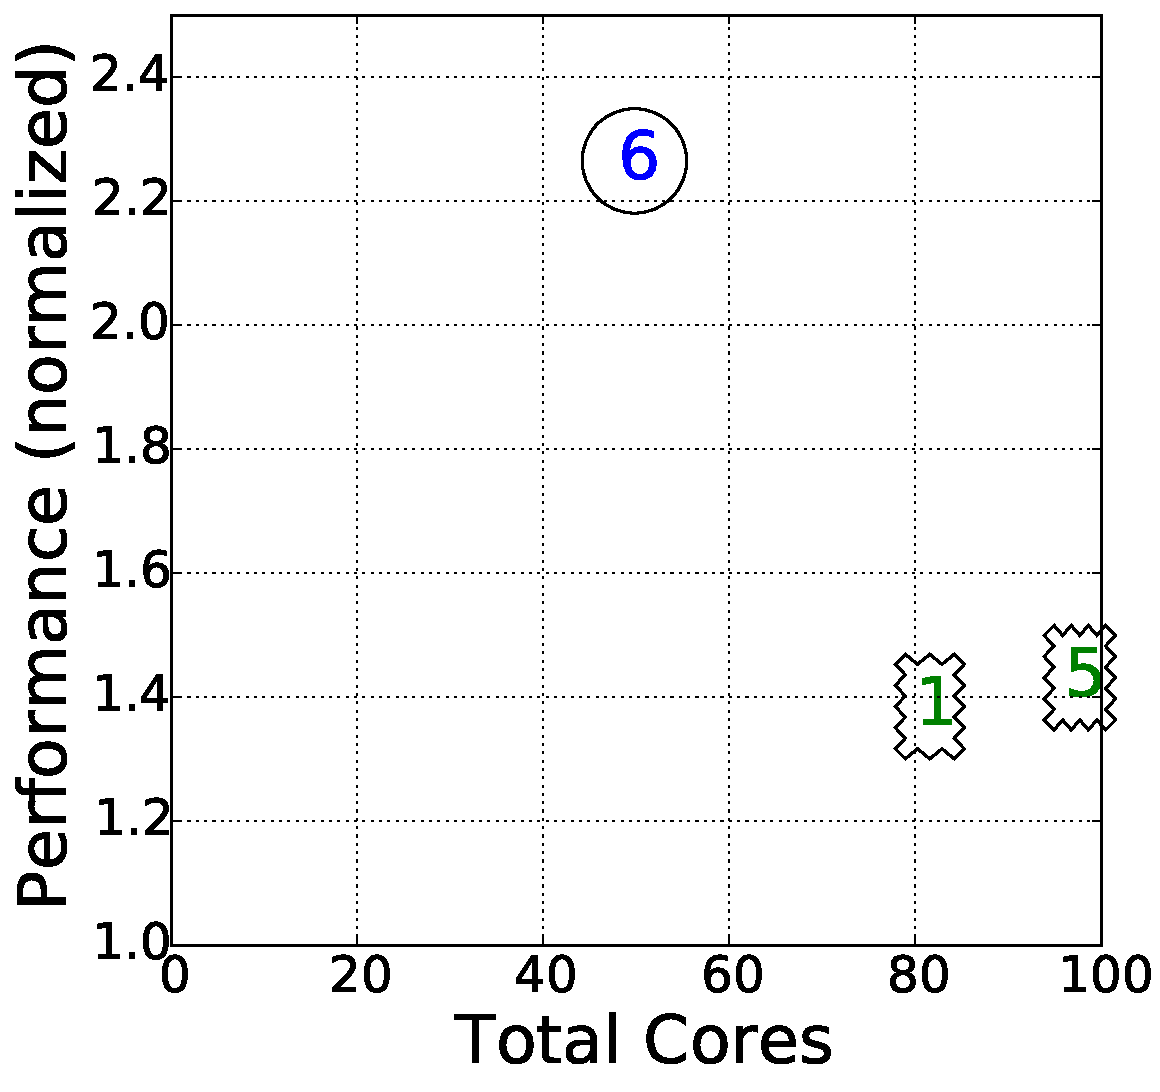
\includegraphics[width=\linewidth]{figures/multiple_bo_time_spark1.5.regression.huge_12_cores.pdf}
    \caption{\cherrypick}
    \label{fig:search_time_cherrypick}
\end{subfigure}
\begin{subfigure}[b]{0.4\textwidth}
    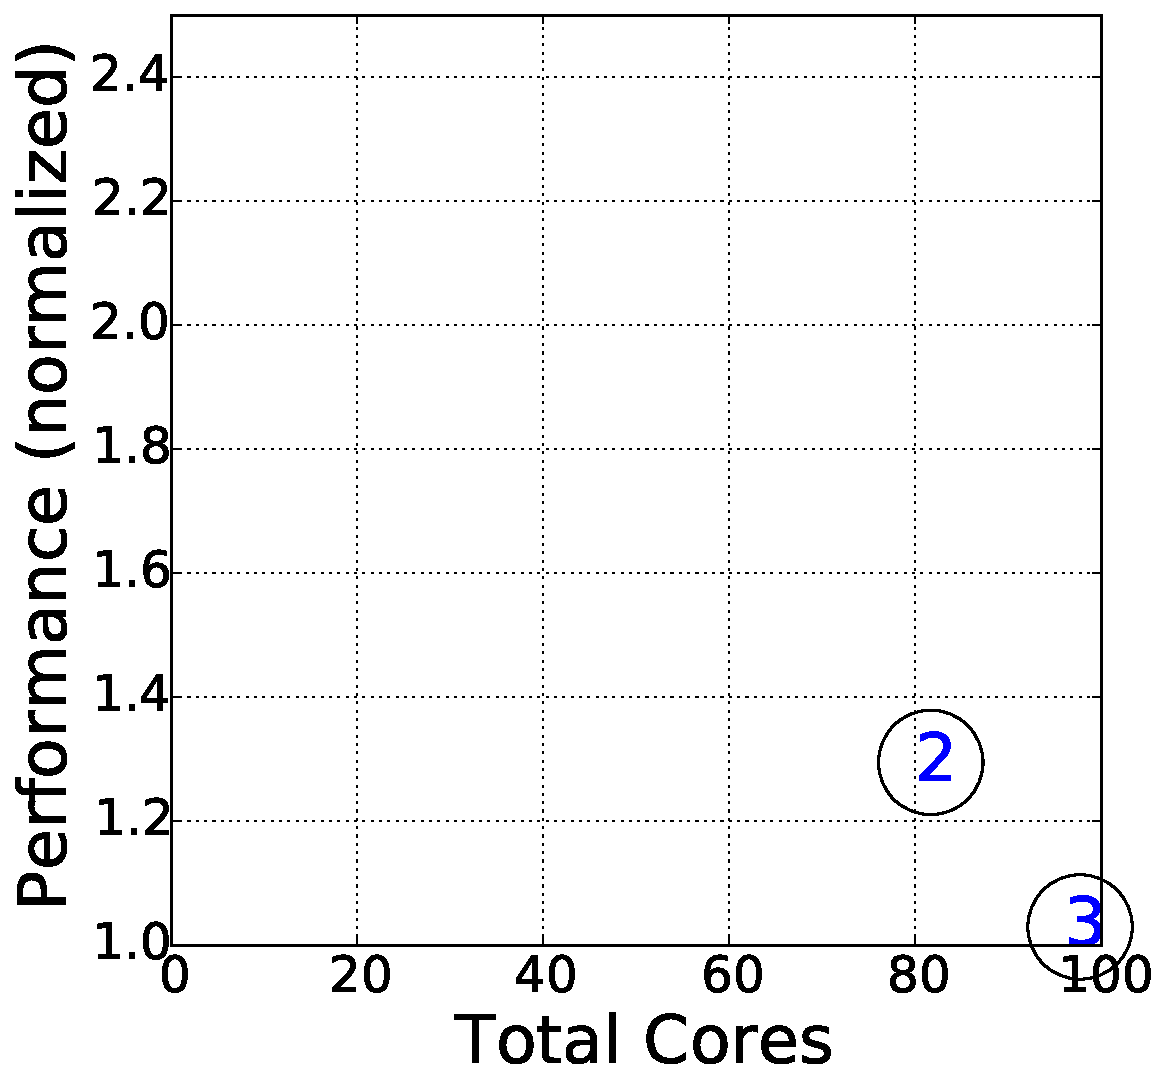
\includegraphics[width=\linewidth]{figures/multiple_scout_time_spark1.5.regression.huge_24_m4.large_cores.pdf}
    \caption{\scout}
    \label{fig:search_time_scout}
\end{subfigure}
\caption{\small{\textbf{Minimizing execution time of Regression on Spark.} Since the Regression workload requires both computation and large memory, \scout directly chooses configurations with the \emph{r4} family and larger cores.}}
\label{fig:compare_2}
\end{figure}

\subsubsection*{Reliable exploration is difficult and generates high search cost}
In Figure~\ref{fig:compare_2},~\ref{fig:compare_3},~\ref{fig:compare_1},~\ref{fig:compare_4}, we observe that the search path generated by \emph{CherryPick} involves more distinct VM types due to the need to explore the performance model. For example, in Figure~\ref{fig:compare_3}, CherryPick visits each instance family at once in all examples while \scout skips some specific families.
This is because \scout builds the performance model from historical data. Hence, it requires only little (or no) exploration. This phenomenon, exploration-exploitation dilemma, is studied extensively in Machine learning~\cite{kaelbling1996reinforcement}. The cold-start issue (as described in Section~\ref{sec:motivation} arises partly because of the requirement to explore the configuration space since \scout learns the performance behavior from historical data from workloads (previously explored) can sidestep the need to explore the search space.




\subsubsection*{Fragility of CherryPick}
As explained in Section~\ref{sec:motivation}, CherryPick is fragile
because it is sensitive to its parameters and the starting points.
In the four examples, \emph{CherryPick} starts from the same three configurations; however, the results are very different.
In \myfigure{\ref{fig:compare_3}}, \emph{CherryPick} fails to characterize the search space, which results in long search path (and high search cost).
While in \myfigure{\ref{fig:compare_4}},
\emph{CherryPick} stops too early and only finds a local minima (the $c4$ family).
These two examples show that \emph{CherryPick} is fragile and therefore, its search performance is not stable.

\subsubsection*{\scout identifies resource requirements}
When resource requirements can be articulated, a search process is more likely to find cloud configurations effectively and efficiently. In \myfigure{\ref{fig:compare_1}},
the \emph{PageRank} workload runs faster on a larger cluster (higher core counts) and higher-frequency CPUs. The \emph{r4} family, with larger memory but slower CPU speed, does not seem to be the best choice, hence avoided by \scout and instead prefers \emph{c4} and \emph{m4} family.
This tendency is more clear in the other cases as well (Figure~\ref{fig:compare_2}, ~\ref{fig:compare_3}, and~\ref{fig:compare_4}).


\begin{figure}[!htbp]
\centering
\begin{subfigure}[b]{0.4\textwidth}
    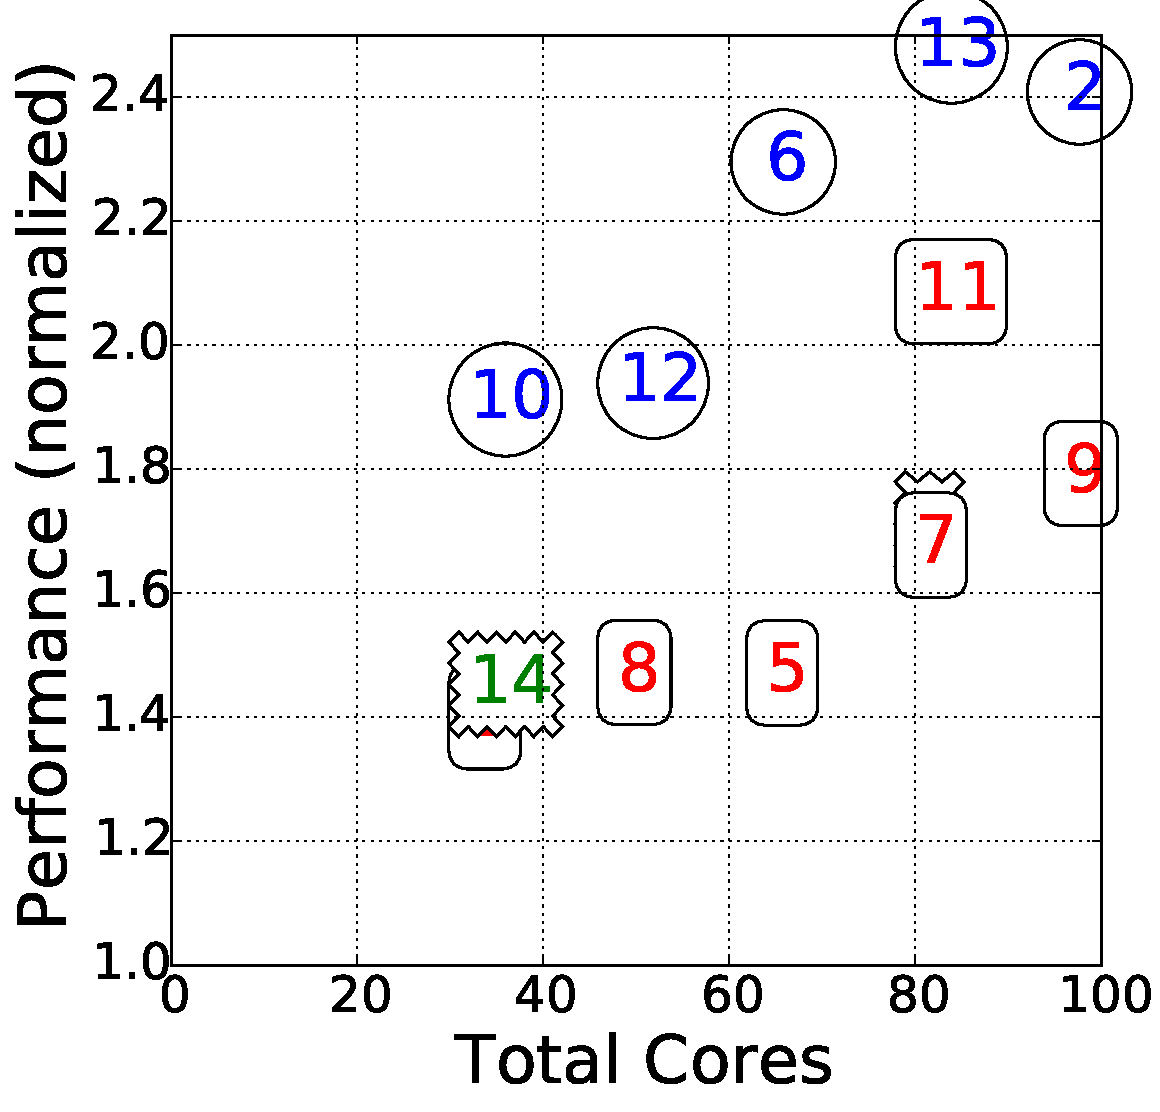
\includegraphics[width=\linewidth]{figures/multiple_bo_cost_hadoop.terasort.bigdata_12_cores.pdf}
    \caption{\cherrypick}
    \label{fig:search_cost_cherrypick}
\end{subfigure}
\begin{subfigure}[b]{0.4\textwidth}
    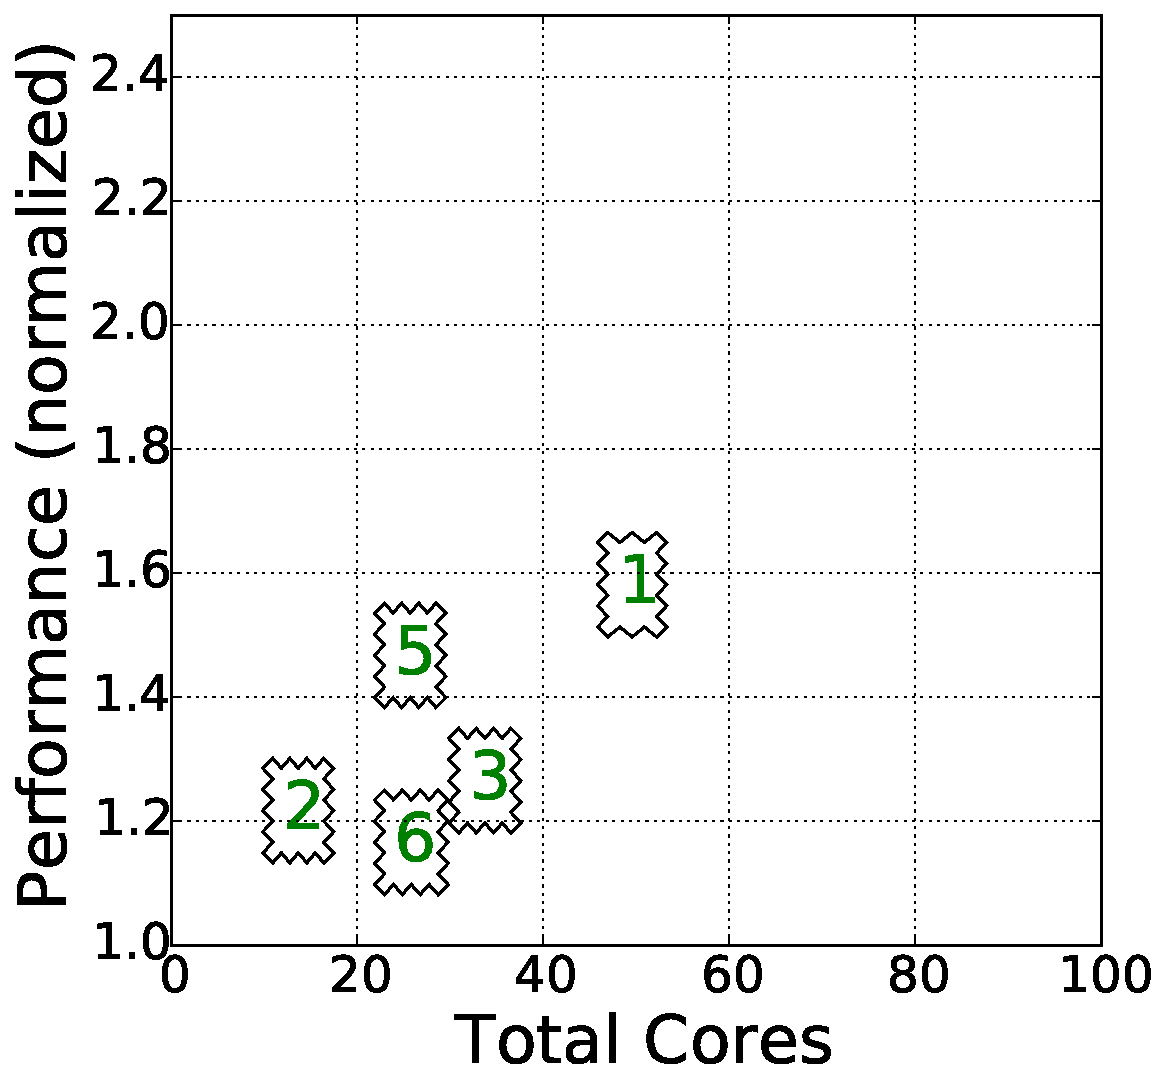
\includegraphics[width=\linewidth]{figures/multiple_scout_cost_hadoop.terasort.bigdata_24_m4.large_cores.pdf}
    \caption{\scout}
    \label{fig:search_cost_scout}
\end{subfigure}
\caption{\small{\textbf{Finding the cheapest configuration for Terasort on Hadoop.} The Terasort workload requires enough memory to avoid spilling data to disks. Besides, a large cluster can be insufficient due to the shuffle phase in MapReduce.  \scout chooses a smaller cluster with the general-purpose VM type. }}
\label{fig:compare_3}
\end{figure}



\subsubsection*{\scout captures the complex cost model}
In a real-world setting, practitioners can choose either a smaller cluster built using more powerful instances or choose large cluster built using smaller or less powerful instances (a scale-out and a scale-out configuration). The performance model used by \scout can infer the size of the cluster of the best cloud configuration.
In \myfigure{\ref{fig:compare_3}}, \scout chooses to run \emph{TeraSort} on a smaller cluster to save cost. On the contrary, in Figure~\ref{fig:compare_4}, \scout selects a larger cluster for efficiently running the \emph{Naive-Bayes} workload while achieving lower cost. These two examples show that \scout captures the complex relationship between the resource metrics and the running cost.


\subsubsection*{Summary}
The main difference between \emph{CherryPick} and \scout lies how the method explores the space of possible cloud configuration options. We can see that \emph{CherryPick} has to explore more cloud configuration options and hence have higher search cost (longer search path) while \scout searches within a relatively restricted region. This feature of \scout can be attributed to its performance model, which learns from the historical data. This also goes to show that encoding scheme, which uses low-level performance metrics, is successful in transferring knowledge from one workload to another.



\section{Discussion}
\label{sec:discussion}


\subsection*{Tuning Searching Performance}

\scout uses ``probability threshold'' and ``misprediction tolerance'' as stopping criteria.
%We examine how they affect the search performance of \scout.\\

\subsubsection*{Probability Threshold}
\scout chooses the next configuration to evaluate
based on the probability of improvement and
stops when the probability is lower than the probability threshold $\alpha$.
\myfigure{\ref{fig:single_probability_threshold}} shows that
a higher probability threshold is pessimistic and 
terminates the search process prematurely,
hence, shorter search path
and unstable search results). 
The probability threshold presents a trade-off between
search performance and search cost.
The right threshold must consider
the reliability curve of classification methods~\cite{niculescu2005predicting}.

\subsubsection*{Misprediction Tolerance}
\scout terminates the search process if the selected configurations do not improve the current best choice (considered as a misprediction).
\scout maintains a counter of mispredictions.
A higher limit tolerates more mispredictions but yields better search performance due to more chances.
A proper limit should consider both
the size of search space and the accuracy of prediction.
In \myfigure{\ref{fig:single_misprediction_tolerance}},
we show that a higher tolerance level leads to better search performance but higher search cost.
This trade-off is similar to the probability threshold.

\begin{figure}[!htbp]
\centering
\begin{subfigure}[b]{0.4\textwidth}
    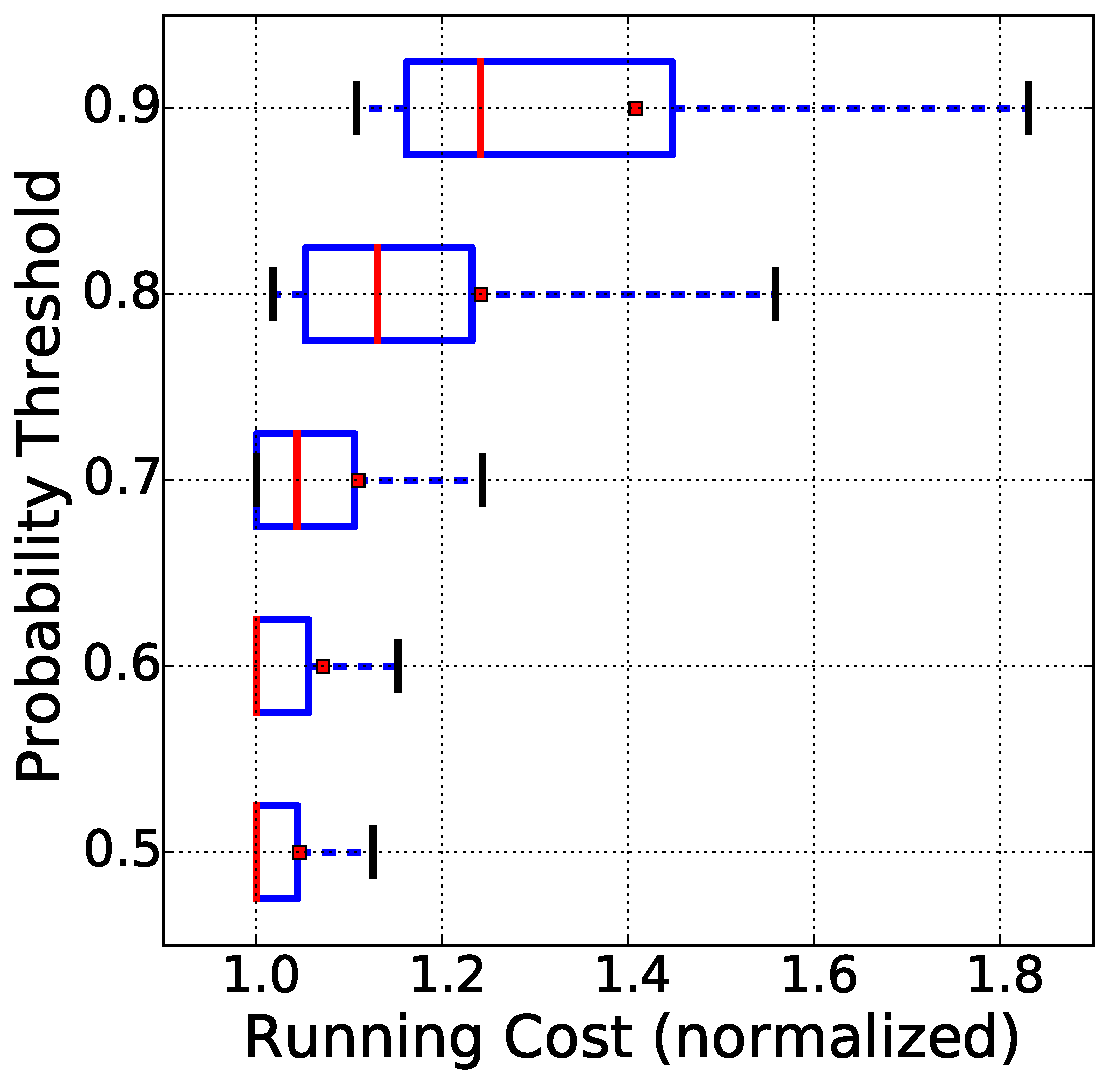
\includegraphics[width=\linewidth]{figures/single_cost_tuning_probability_performance.pdf}
    \caption{Search Performance}
    \label{fig:single_cost_tuning_threshold_performance}
\end{subfigure}
\begin{subfigure}[b]{0.4\textwidth}
    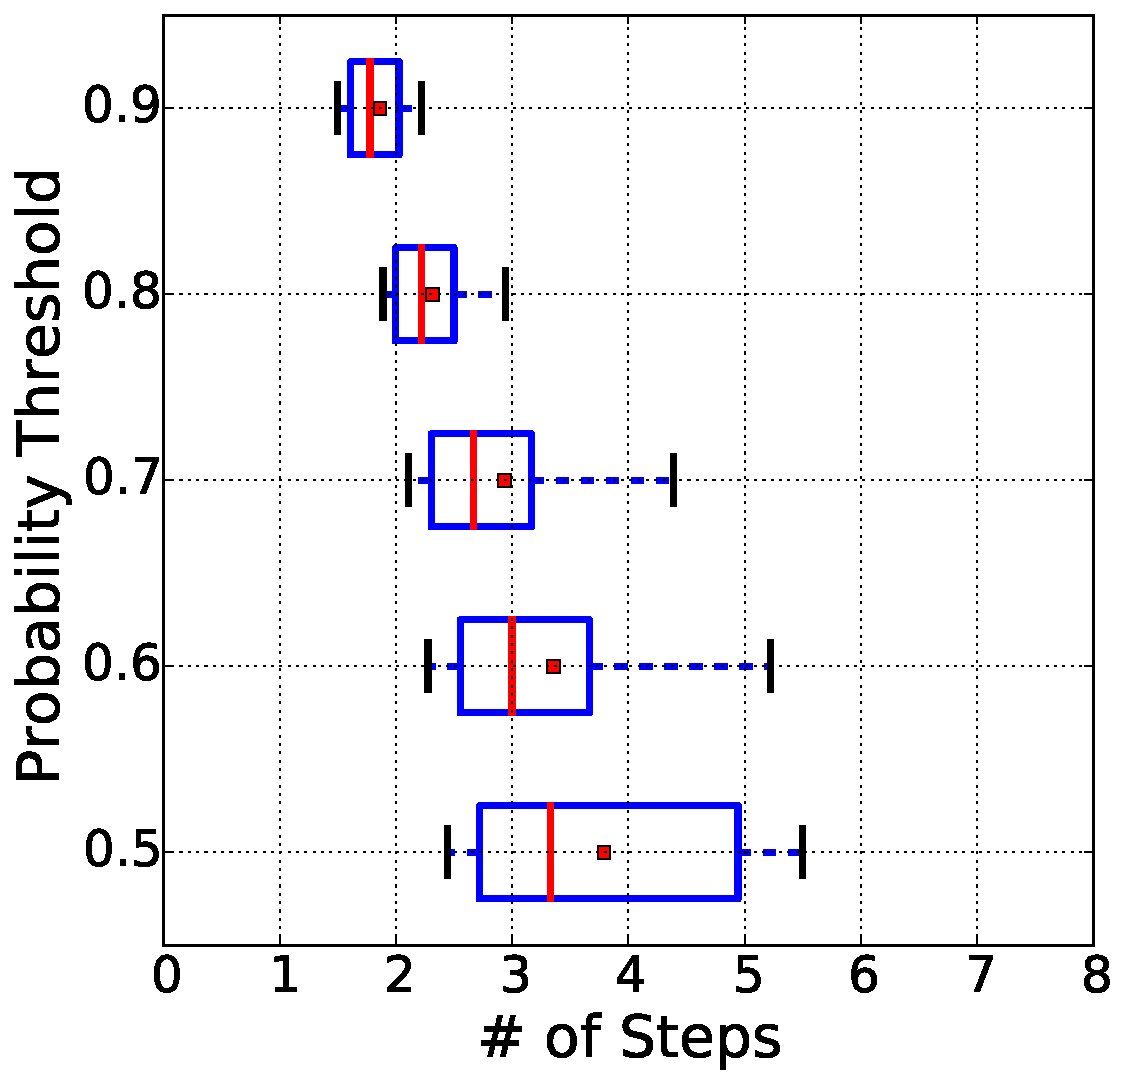
\includegraphics[width=\linewidth]{figures/single_cost_tuning_probability_steps.pdf}
    \caption{Search Cost}
    \label{fig:single_cost_tuning_threshold_steps}
\end{subfigure}
\caption{\small{\textbf{Tuning the probability threshold.} A smaller threshold generates a longer search path but ensures better search performance.}}
\label{fig:single_probability_threshold}
\end{figure}

\begin{figure}[!htbp]
\centering
\begin{subfigure}[b]{0.4\textwidth}
    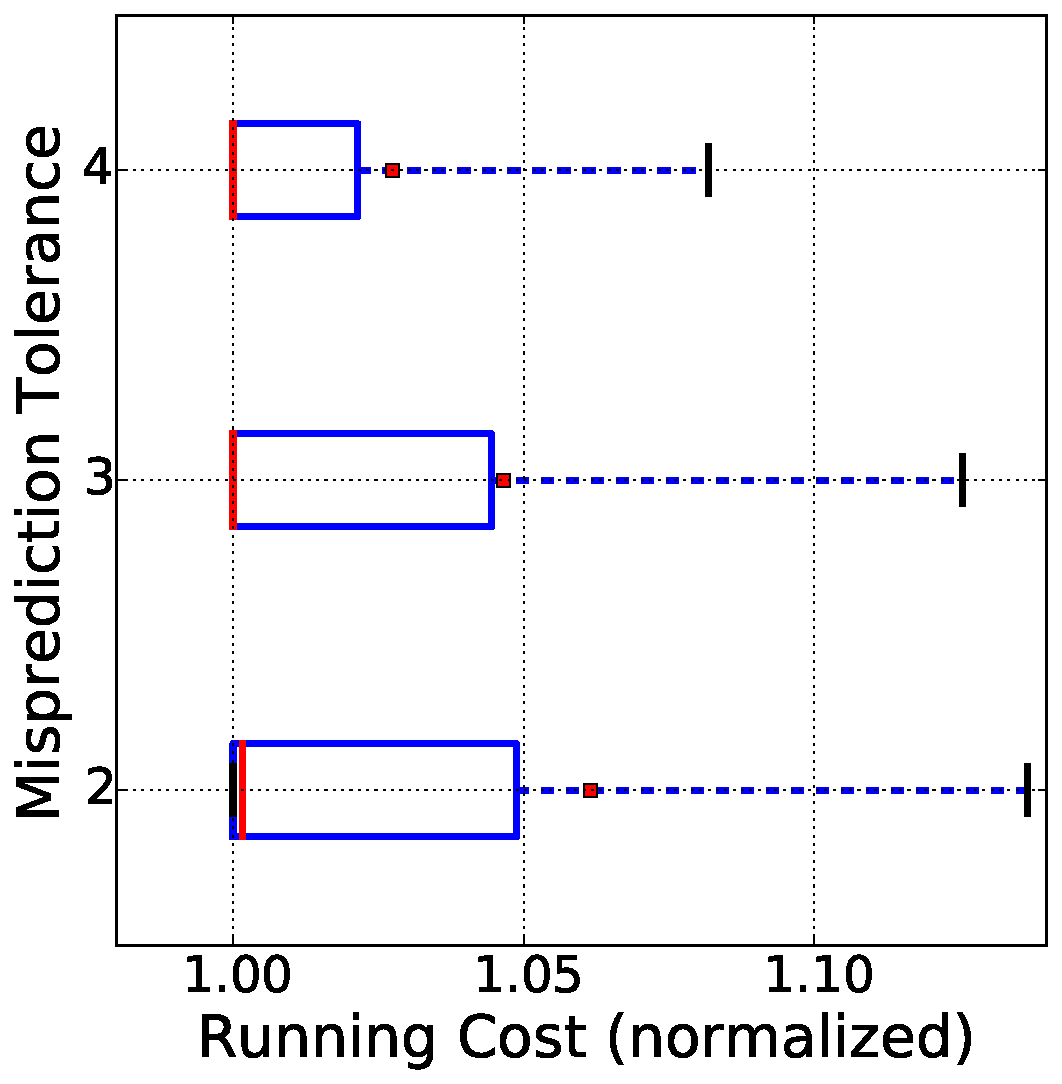
\includegraphics[width=\linewidth]{figures/single_cost_tuning_tolerance_performance.pdf}
    \caption{Search Performance}
    \label{fig:single_cost_tuning_tolerance_performance}
\end{subfigure}
\begin{subfigure}[b]{0.4\textwidth}
    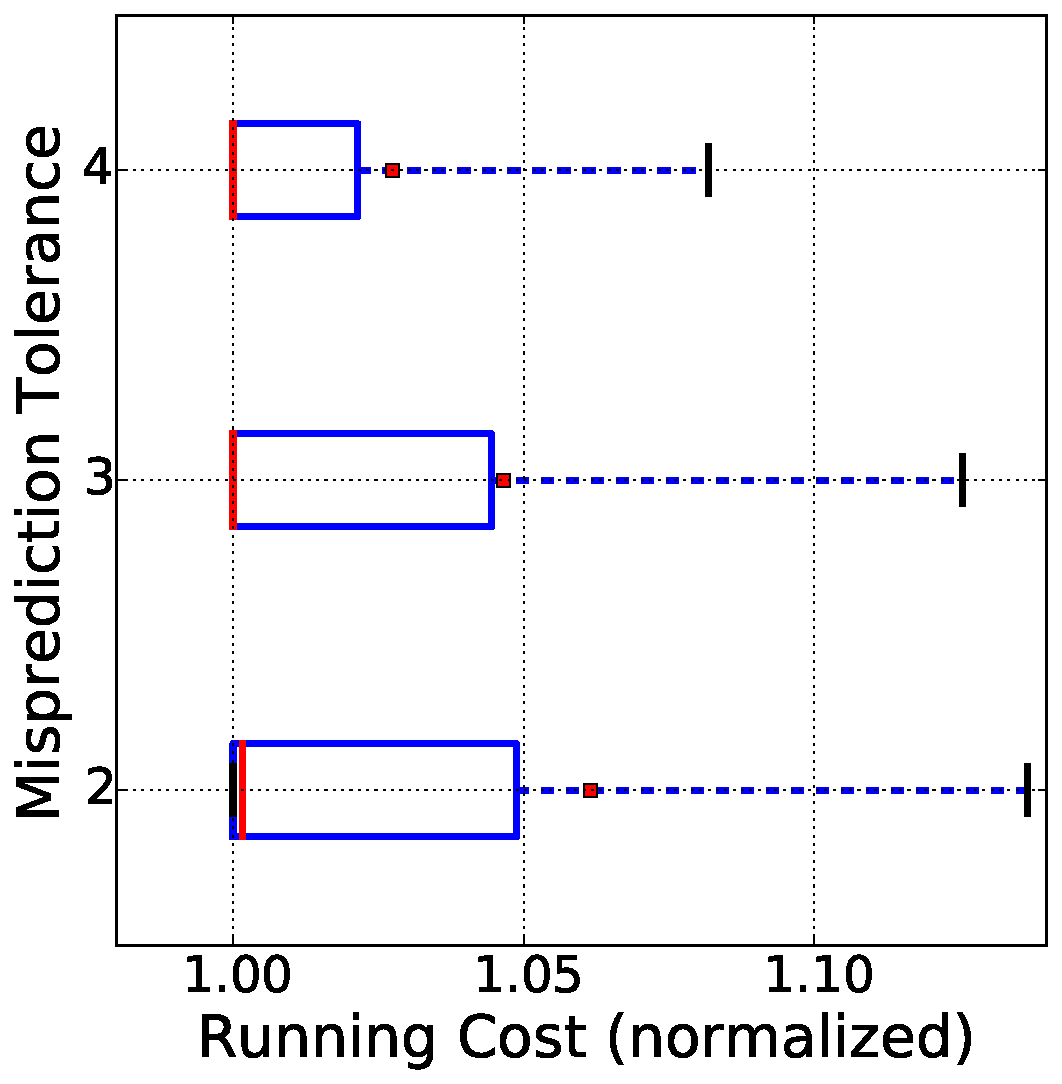
\includegraphics[width=\linewidth]{figures/single_cost_tuning_tolerance_performance.pdf}
    \caption{Search Cost}
    \label{fig:single_cost_tuning_tolerance_performance}
\end{subfigure}
\caption{\small{\textbf{Tuning the misprediction tolerance.} A higher tolerance to mispredictions generates higher search cost.}}
\label{fig:single_misprediction_tolerance}
\end{figure}


\subsection*{Alternative search strategies}
\scout generates the probability vector $P_{i}$
for each new observation (running the workload on $S_i$).
Our current search strategy only uses information from the latest observation.
\scout stores historical observations and therefore,
the next search step can be determined using several past observations.
%In \myfigure{\ref{fig:search_strategies}}, we illustrate a way to incorporate other observations.
Given two observations on $S_1$ and $S_2$ and two unevaluated configuration $S_3$ and $S_4$,
\scout generates prediction probability
$P_{13}$ and $P_{14}$ from $S_1$, and $P_{23}$ and $P_{24}$ from $S_2$.
Instead of choosing $P_{23}$ after the second step,
\scout should choose $P_{14}$ when $S_2$ is much worse than $S_1$ (due to mispredictions).
This strategy is more likely to avoid bad choices.
On the other hand, 
\scout currently relies on offline performance modeling.
Another alternative is to update the prediction model upon new observations.
For unseen workloads, this update enables \scout to improve prediction accuracy.
However, the downside is the cost of retraining the model.
An online learning method might help reduce the retraining cost.
The two possible alternatives remain as future work.

\begin{figure}[!htbp]
 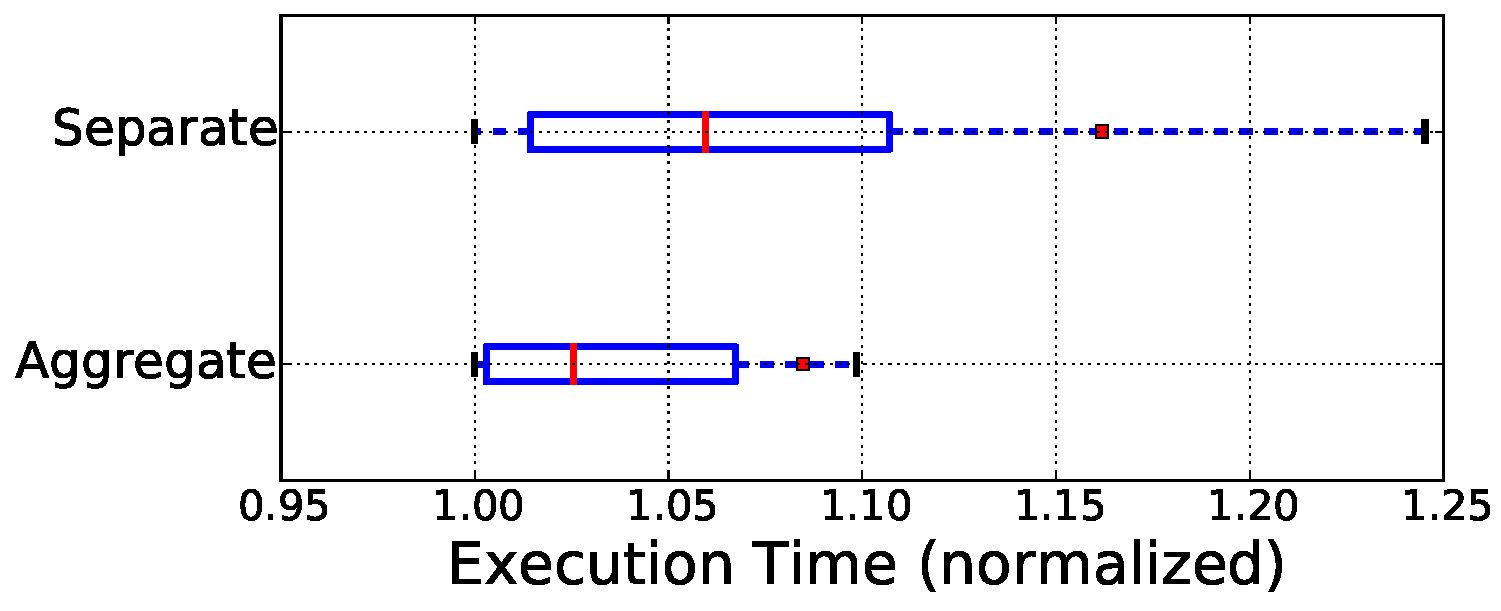
\includegraphics[width=.8\textwidth]{figures/multiple_size_of_dataset.pdf}
 \centering
 \caption{\textbf{Universal performance models.}
 Training data form multiple systems improves prediction.}
 \label{fig:prediction_accuracy_comparison}
\end{figure}

\textbf{Universal Prediction Models.}
% The performance models are built to find the best cloud configuration for a certain workload. These performance models generalize the information learned from the evaluated configurations. This helps the model to be accurate while predicting new cloud configurations. 
In prior work, the performance model needs to be retrained
for every optimization process, which leads to wasted effort.
There is a need for a modeling strategy, which becomes more accurate with experience. 
% This experienced model is useful in our setting, since measuring a new cloud configuration can be resource intensive. 
Transfer learning can be beneficial in our setting,
where the performance model can predict a new workload
using knowledge learned from optimization results of other workloads~\cite{pan2010survey}.
\scout tries to learn from other performance data so that all the experience from the past optimization process is not lost.
Figure~\ref{fig:prediction_accuracy_comparison} shows
how the performance model learned from more data (from different workloads) can
generalize better than the performance model training for a single application.
In the figure, the horizontal axis represents the execution time of the workload,
and the vertical axis shows two versions of \scout. \emph{Separate}
refers to the \scout which is trained with performance data from just
Hadoop workloads, whereas \emph{Aggregate} refers to \scout trained on Hadoop
as well as Spark workloads. We can see that \emph{Aggregate} can find cloud
configurations with better performance (lower execution time). 
\textit{Overall, the prediction model used in \scout is universal and can learn from any workload.}

\subsection*{Time-cost trade-off}
Often a
user is willing to wait longer for a result if there is a big
reduction in cost.
For example, many might be willing to trade a 20\% increase execution time for a 50\% decrease in running cost.
This is similar to the energy-time trade-off in high-performance computing~\cite{Freeh2007}.
\scout can support this scenario.
In our design, we define prediction classes based on the normalized performance of a single performance measure, \ie{time or cost}.
Previous work supports this trade-off in a similar manner~\cite{Hsu2018Arrow}.
%We instead define the classes based on the normalized performance of the product of time and cost.
%In our previous work, we show that how to support time-cost trade-off in a search-based method~\cite{Hsu2018Arrow}.
%We plan to support this feature in \scout.


\section{Conclusion}
\label{sec:conclusion}

Cloud architecture tuning (CAT) is essential
to maximize the performance of an application
while keeping the deployment cost down.
In this chapter, we identify key elements for an effective CAT method.
We design and implement a novel system \scout, which delivers
\emph{efficient}, \emph{effective} and \emph{reliable} search performance.


%Today most applications are hosted in the cloud.
%It is essential to maximize the performance of an application while keeping the deployment cost down.
%Machine learning and sampling techniques have been previously proposed to
%build models to predict the performance of cloud configurations.
%However, the techniques proposed in prior work are either expensive to train or are unreliable---if trained on %sparse samples. 

%Our method, \scout, is different to the previously proposed directions and promotes learning from previous %experience---optimization process.
%We advocate using historical data to identify regions on the configuration space, which might contain the best cloud configuration. To use the historical data, we propose a new modeling scheme which use low-level metrics along with pair-wise modeling technique to transfer knowledge from one optimization process to the other.


\chapter{Finding faster configurations using flash}
\label{chapter:flash}

This chapter presents an approach to estimating end-to-end performance
of distributed storage systems.
We explain why low-level performance metrics are a desirable proxy
for estimating end-to-end performance.
We then present our automatic model building tool for generating
robust and accurate performance models.

% \section{Introduction}
\label{ch4:sec:introduction}

Many storage systems are moving away from dedicated appliance-based storage model to software-defined 
storage (SDS), which separates software that provisions and manages storage from the hardware that provides raw physical storage~\cite{sds_att, Thereska2013, Jalaparti2012}.
This trend is partly driven by the tremendous growth of data and the emergence of cloud applications that operate in a multi-tenant environment with diverse workload characteristics.
As a result, the rigid appliance-based model, with tightly-coupled hardware and software features, is no longer cost-effective, lacks flexibility, and does not scale well.
SDS systems are increasingly abandoning centralized storage services in favor of distributed systems like Ceph~\cite{ceph}, HDFS~\cite{hadoop}, Swift~\cite{openstack}. 
Distributed storage systems are attractive because they scale well, allowing storage services to grow or shrink, based on storage demands. 
They are also better suited to handle diverse multi-tenant workloads. 

Providing reliable quality of service (QoS) to storage applications is critical in an SDS environment shared by multiple applications 
with diverse usage patterns. However, in a distributed storage environment, it is challenging to provide storage QoS in a consistent 
and reliable manner. Practical deployments of modern distributed storage systems like Ceph are composed of a large number of 
individual storage components that can interact in a complex manner. 
Diverse and time-varying storage workloads and performance interference in a multi-tenant environment further 
complicate the reliable assurance of storage QoS. Reliable and accurate monitoring of 
high-level storage performance metrics (e.g. throughput and IOPS) is critical 
for providing storage QoS guarantees.    
However, monitoring end-to-end storage performance is difficult in a distributed storage service. 
Instrumenting user applications to measure storage performance is not always practical. 
Performing benchmark tests in production systems also has practical limitations since they 
interfere with storage application workload.
Furthermore, running exhaustive benchmark experiments to cover diverse application workloads, 
deployment topologies, and large configuration parameter space is time-consuming and impractical in many cases. 
Building accurate analytical performance models, on the other hand, is also difficult for the reasons mentioned above.
 
This chapter proposes the idea of using low-level system metrics (e.g., CPU usage, RAM usage and network I/O)
as a proxy for measuring high-level performance (e.g., end-to-end IOPS and throughput) of 
distributed storage applications.
We design, implement and evaluate a practical tool, called \emph{Inside-Out}, that applies 
machine learning techniques to the low-level metrics collected from individual components 
of a distributed storage system to accurately estimate high-level storage performance metrics---like throughput and IOPS---of the entire 
distributed storage system.
We believe that a tool like Inside-Out can serve as an important component of the overall SDS architecture.

Inside-Out takes a black-box modeling approach, which does not require knowledge about distributed storage system protocol, workload characteristics, and deployment topology. 
Inside-Out relies upon machine learning techniques to automatically derive an accurate end-to-end performance model.
We explore several well-known machine learning algorithms including linear regression, 
decision tree learning, and ensemble methods \cite{Wang2004, Noorshams2013}, and conclude that  
there does not exist an one-size-fits-all algorithm that can work in all prediction cases.
Hyperparameter tuning \cite{Chapelle2002, Noorshams2013}, model selection \cite{Kohavi1995} and 
feature selection \cite{guyon2003introduction, Saeys12007} all turn out to be too complicated for optimizing prediction accuracy.
In contrast, Inside-Out uses a two-level learning method that automatically selects important features, boosts prediction accuracy, and achieves consistent prediction. 
This two-level learning method pipelines two supervised learning algorithms to eliminate irrelevant features while avoiding overfitting problems.\footnote{\label{ft:overfitting}
Overfitting describes the situation when a model captures the relationship of noisy data but not the underlying relationship \cite{domingos2012few}.
Overfitting becomes more prominent in the presence of high dimensional data}

Inside-Out offers several key benefits. 
%[MRA] Unlike traditional analytic performance modeling approach, Inside-Out is generic in nature, and therefore, it can be applied to different storage services.  
Unlike traditional analytic performance modeling approach, Inside-Out is more generic, 
and therefore can be more easily applied to different storage services.  
Different from previous work, Inside-Out 
does not require information about system configuration and application workload~\cite{Ruemmler1994, Shriver1998, Wang2004, Kelly2004, Yin2006, Noorshams2013, Ardagna2014}. 
Due to the self-learning property, \emph{Inside-Out} improves performance prediction accuracy with more data.
It can also adapt to changes in the system
by continuously learning the system behavior. 

We evaluate Inside-Out using Ceph~\cite{ceph} %as an example distributed storage system 
running on an OpenStack-based SDS platform.
The low-level performance metrics are collected from participant virtual machines 
running various components of a Ceph storage service.\footnote{\label{ft:vm}
Our approach is not limited to VM-based environments.
It can be applied to container-based and bare-metal storage servers as well.
}
Our in-depth evaluation shows that Inside-Out generates end-to-end performance models with 91.1\% prediction accuracy on average.
More importantly, as discussed above, Inside-Out is generic in nature as it captures the behavior of the storage system 
by analyzing low-level system metrics (that are protocol and application agnostic). Furthermore, we demonstrate that Inside-Out 
%[MRA] can provide reliable performance monitoring even in the presence of evolving workload characteristics, changing storage 
can provide reliable hints for performance monitoring tasks even in the presence of evolving workload characteristics, changing storage 
configuration and interfering tenants. We also show that Inside-Out is reliable in estimating end-to-end performance 
even when the storage system expands or shrinks.
We show that Inside-Out provides reliable performance 
prediction when the storage system is up to four times larger than the one used for building machine learning models during 
the training phase. 
Lastly, Inside-Out is able to learn new storage behavior over time.
% \section{Mapping from Low to High}
\label{sec:challenges}

%[commented by MRA] We discuss how to use low-level performance metrics collected from distributed components to build an accurate end-to-end performance model for a distributed storage system in the SDS environment.
This section discusses the guiding principles and challenges in using low-level performance metrics
to build accurate end-to-end performance models for a distributed storage system.
%collected from individual components of a 
%distributed storage system for building an accurate end-to-end performance model.

%\subsection{Searching for Representative Features}
\subsection{Important Considerations}

This section describes how we use low-level performance metrics
to predict high-level system performance.
We discuss how we pick the metrics and how to transform metrics
to meaningful features.

\label{sec:feaatures_for_distributed_system}

%[commented by MRA] We have to keep in mind that we are developing a tool that can apply to diverse storage services to be deployed in SDS.
%Manually building models for each storage service requires energy and cost that are several times more than an automatic and general approach.
%Note that we are developing a tool that can be applied to a diverse set of storage systems and services.
%Manually building a model for each storage service requires more effort and cost compared to an automated 
%and general, i.e., application-agnostic, approach.

%\subsubsection{Requiring general performance metrics}
\subsubsection*{General low-level metrics}
%
%Low-level performance metrics are general and application independent.
Since our goal is to provide a tool for estimating the end-to-end performance of a diverse set of 
storage systems, the inputs to our model need to be generic in nature, \ie they need to 
be independent of storage systems or the distributed protocols used by such applications. An SDS provider 
should be able to obtain the input metrics without instrumenting storage application or requiring domain 
knowledge about the storage application. Low-level system metrics (e.g. CPU utilization, memory usage, network IO, etc.) 
satisfy these requirements. DeepDive uses low-level metrics to identify performance anomaly for a running VM~\cite{Novakovic2013}. 
To the best of our knowledge, this work presents the first study that maps low-level system metrics to 
high-level end-to-end performance of a distributed storage service.

%Low-level performance metrics are application independent.
%An SDS provider can obtain this information without instrumenting applications.
%For example, DeepDive~\mra{citation?} use low-level metrics to identify performance anomaly for a running VM \cite{Novakovic2013}.
%To the best of our knowledge, this paper presents the first study that maps low-level performance metrics to high-level end-to-end performance of a distributed storage service.

\begin{figure}
\centering
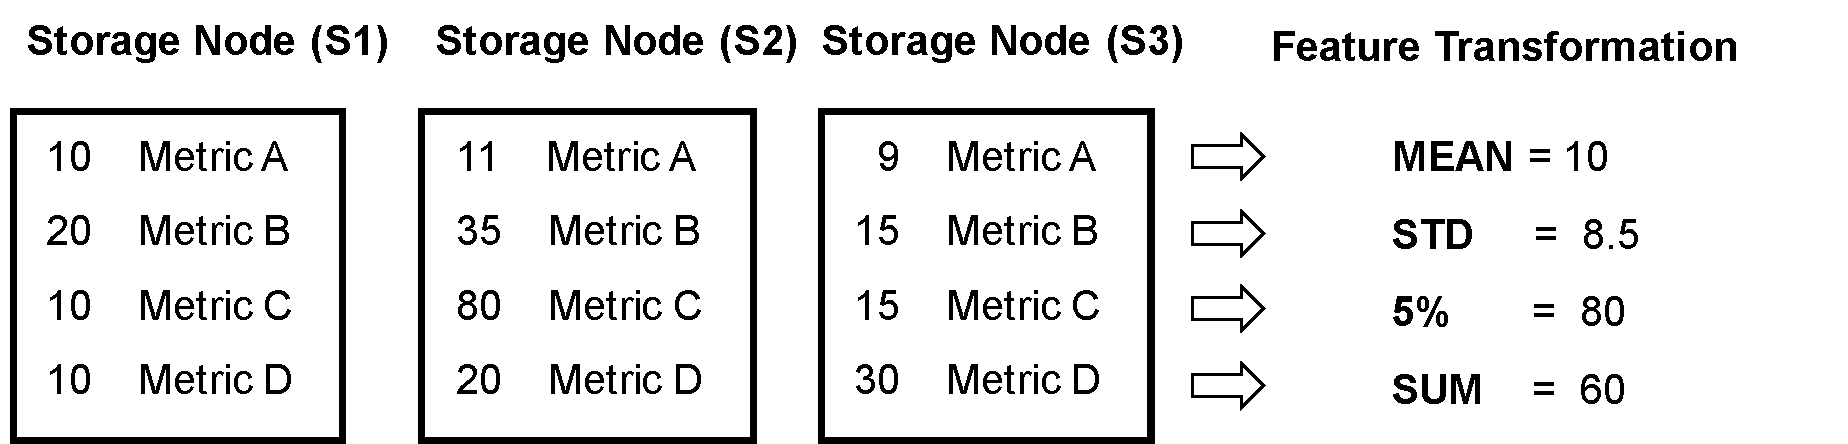
\includegraphics[width=0.9\textwidth, keepaspectratio]{figures/features.pdf}
\caption{Four statistical features used in Inside-Out to capture load and internal status of a distributed storage system.  The numbers and metrics represent low-level performance data collected from storage nodes.}
\label{fig:feature_types}
\end{figure}


%\subsubsection{Handling the distributed system scenario}
\subsubsection*{Capture important features of a distributed storage system}
%
%One important characteristic of a distributed storage system is that it can expand or shrink on demand 
A distributed storage system can dynamically expand or shrink
according to demand.
The performance model has to capture the current 
scale of the deployment, the bottlenecks, and the average and variance in performance
of individual components of the distributed system. For each low-level system metric collected from 
various components of the distributed system, we use four statistical variables to characterize the behavior of a distributed system (see \myfigure{\ref{fig:feature_types}}). 
The statistical variable \textit{mean} and \textit{std} describe whether the impact of the workload is evenly distributed among 
storage components. The \textit{sum} variable represents the scale of the deployment, while the variable \textit{5\%} (top 5 percentile) captures the hot spot situations. 
The feature transformation from raw system metrics to these four statistical values also allows Inside-Out to apply 
the uniform input format for developing performance models for distributed systems at different scales.

\subsection{Feature Selection}
\label{sec:non-deterministic}

In this work, we collect low-level performance metrics
from two components of Ceph
namely monitor (MON) and Object Storage Daemons (OSD).
We use \emph{dstat}, a monitoring tool to collect resource statistics,
to collect 32 low-level performance metrics in total.
These measurements are then transformed using the process described in \myfigure{\ref{fig:feature_types}} (refer to Section~\ref{sec:data_preprocessing} for more details).


Selecting the ``right'' features from high dimensional data
is a challenging task because
as computation complexity increases, prediction accuracy may decreases
~\cite{guyon2003introduction, Saeys12007}.
Furthermore, for our case, the right feature set is not always the identical.
Table \ref{tab:challenge_feature_selection} shows the \emph{model accuracy} of different learning methods when modeling 
read throughput. 
%\chin{
%verified with $10$-fold cross validation.
%}
We see that all learning methods achieve high model accuracy
even though they choose different features. 
The model accuracy was obtained using $k$-fold cross validation (\textit{k}=10),
a common technique for assessing model accuracy. 
The training data is partitioned into $k$ disjoint sets. 
A single data partition is used for validation purpose and the remaining $k-1$ partitions are used for training data.
Although all models yield good model accuracy, they perform poorly and inconsistently when the storage environment changes. 
In \myfigure{\ref{fig:challenge_generalization}},
we show the prediction accuracy under
%we show prediction accuracy when we make
three types of changes in the storage environment---increase in the size of the distributed 
storage system, read workload and individual storage IO request size.
These algorithms (discussed later in Section~\ref{sec:algorithm_selection}) do not yield consistent prediction accuracy any more. 
For example, Lasso can still predict well when workload has changed but Decision Tree cannot.
On the contrary, Decision Tree performs better than Lasso when the size of the storage system increases.
We suspect this is caused by the large feature space, which leads to the overfitting problem \cite{domingos2012few, hastie2005}.
Next, we manually remove most features and select only a few with a trial-and-error strategy.
As shown in \myfigure{\ref{fig:challenge_generalization}}, we see significant improvement in some cases, but not all. 
Since an SDS environment can change over time, it is important for our model to provide consistent prediction accuracy under system changes
such as software reconfiguration and cluster expansion.


\begin{table*}[t!]
\caption{Important features selected by different algorithms are not deterministic}
\centering
\label{tab:challenge_feature_selection}
%\begin{tabular}{|lll|lll|lll|lll|lll|}
%\resizebox{!}{.8\linewidth}{
\resizebox*{\textwidth}{!}{
\begin{tabular}{|lll|lll|lll|lll|lll|}
%\begin{tabularx}{1.0\linewidth}{|lXl|lXl|lXl|lXl|lXl|}

\hline
\multicolumn{3}{|c|}{\textbf{Lasso}}   & \multicolumn{3}{c|}{\textbf{Ridge}}   & \multicolumn{3}{c|}{\textbf{Elastic Net}} & \multicolumn{3}{c|}{\textbf{Decision Tree}} & \multicolumn{3}{c|}{\textbf{Random Forest}} \\
\hline
osd  & network.send  & sum  & \textbf{osd}  & \textbf{network.recv}  & \textbf{mean} & osd   & network.send   & sum    & osd    & disk.read       & sum    & osd    & disk.read       & sum    \\
osd  & disk.writ     & sum  & \textbf{osd}  & \textbf{disk.read}     & \textbf{5\%}  & osd   & disk.writ      & sum    & osd    & network.send    & sum    & osd    & network.send    & sum    \\
\textbf{osd}  & \textbf{cpu.sys}       & \textbf{sum}  & \textbf{osd}  & \textbf{load.15m}      & \textbf{std}  & osd   & disk.read      & sum    & osd    & network.recv    & sum    & osd    & disk.writ       & sum    \\
osd  & io.read       & sum  & osd  & network.send  & sum  & osd   & cpu.sys        & sum    & osd    & disk.writ       & sum    & \textbf{osd}    & \textbf{network.recv}    & \textbf{sum}    \\
osd  & vm.minpf      & mean & osd  & tcp.tim       & std  & osd   & tcp.lis        & sum    & \textbf{mon}    & \textbf{memory.buff}     & \textbf{mean}   & osd    & memory.cach     & sum    \\
\textbf{mon}  & \textbf{memory.used}   & \textbf{5\%}  & osd  & network.recv  & std  & osd   & io.read        & std    & osd    & cpu.sys         & sum    & osd    & memory.buff     & mean   \\
\textbf{mon}  & \textbf{memory.cach}   & \textbf{5\%}  & osd  & load.5m       & std  & osd   & io.read        & sum    & osd    & vm.alloc        & sum    & osd    & memory.buff     & 5\%    \\
osd  & tcp.lis       & sum  & osd  & cpu.idl       & sum  & osd   & vm.minpf       & mean   & osd    & vm.minpf        & 5\%    & mon    & io.writ         & sum    \\
osd  & io.read       & std  & osd  & cpu.wai       & sum  & osd   & io.writ        & mean   & \textbf{mon}    & \textbf{cpu.idl}         & \textbf{std}    & osd    & memory.buff     & sum    \\
osd  & io.writ       & mean & osd  & cpu.sys       & sum  & \textbf{mon}   & \textbf{memory.used}    & \textbf{sum}    & mon    & memory.cach     & sum    & mon    & vm.free         & sum    \\
\hline
\multicolumn{3}{|c|}{96.20\%} & \multicolumn{3}{c|}{96.60\%} & \multicolumn{3}{c|}{96.18\%}     & \multicolumn{3}{c|}{96.78\%}       & \multicolumn{3}{c|}{96.94\%} \\
\hline
\end{tabular}
%\end{tabularx}
}
\end{table*}



\begin{figure*}
    \centering
    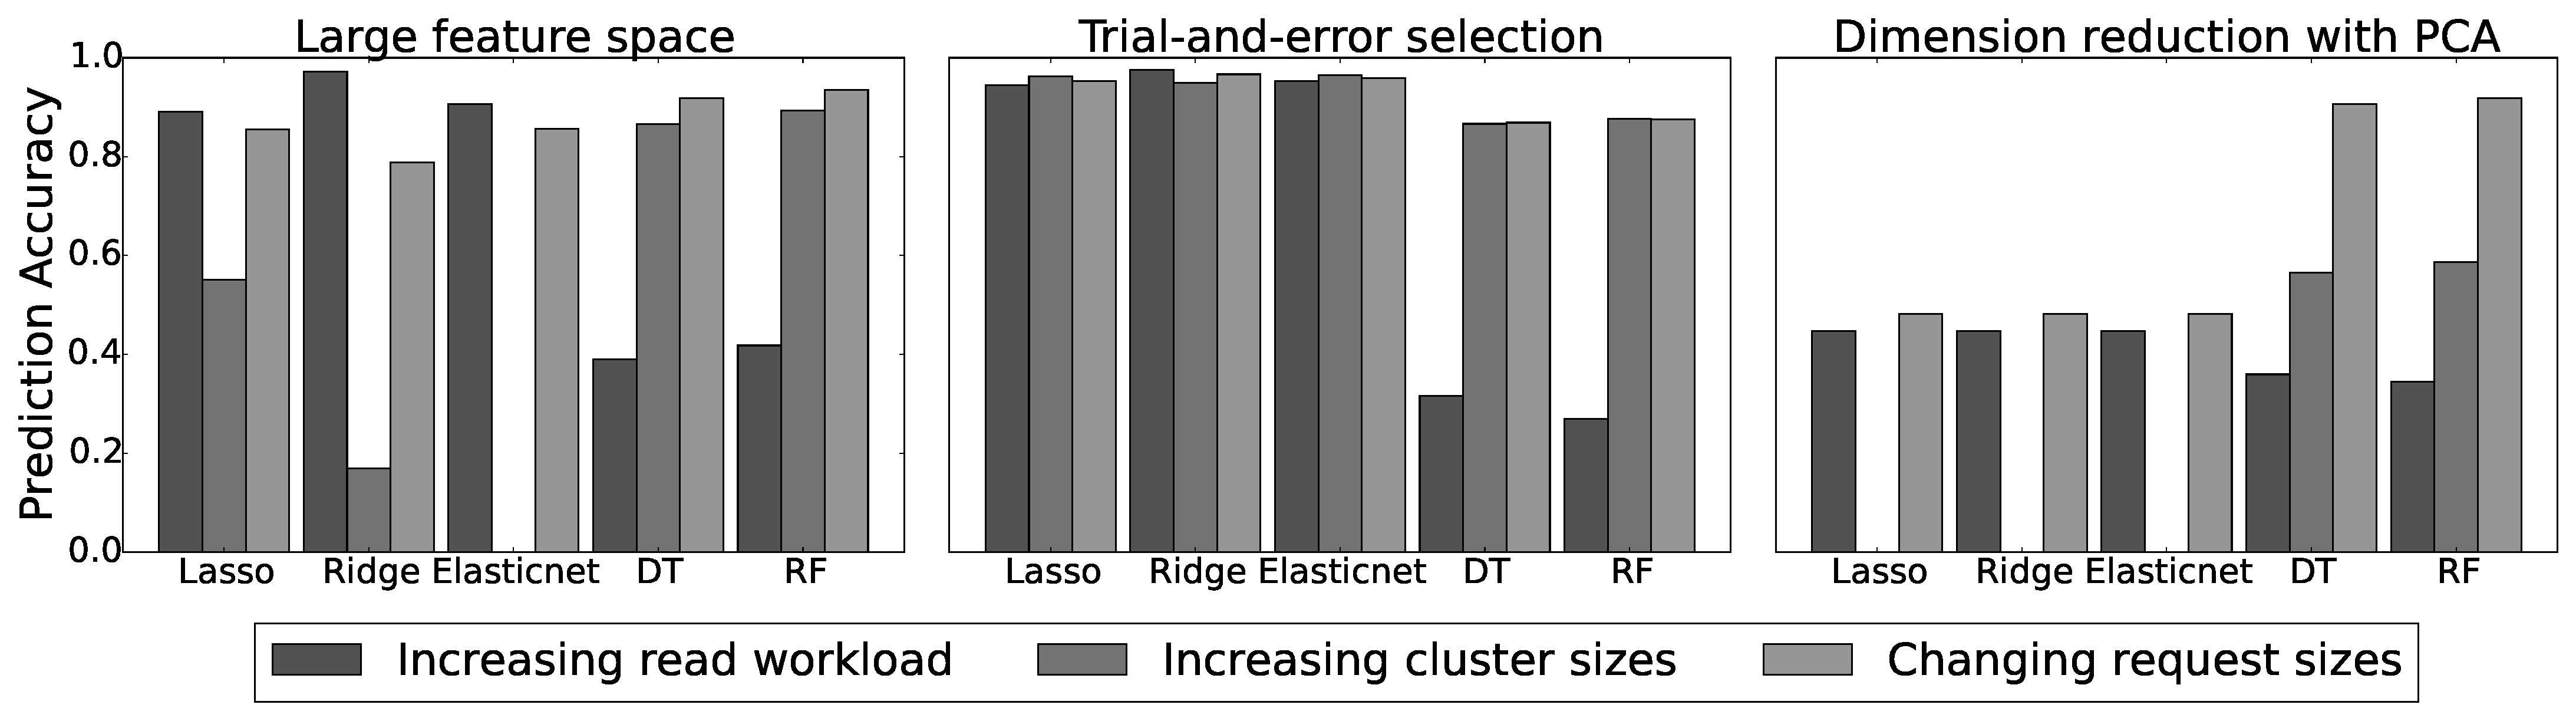
\includegraphics[width=1\textwidth]{figures/challenge_generalization_combined_horizental.eps}
    \caption{Prediction accuracy is inconsistent due to the large feature space.
    Learning methods fail to select the right features in some cases.
    Dimension reduction (PCA with 10 components) does not help in this case.
    In the trial-and-error case, we select a subset of metrics, e.g. \emph{mean(disk.read)}, \emph{sum(network.recv)} and \emph{std(cpu.usr)}.}
    \label{fig:challenge_generalization}
\end{figure*}

Although Hyperparameter tuning, model selection, and 
feature selection have been proposed as potential solutions, it is challenging 
to use them in practice, not to mention the complexity of automating this task. 
PCA (Principle Component Analysis) is another potential solution \cite{Shlens2003}.
PCA transforms original data into a lower dimension while keeping high fidelity.
However, PCA has several limitations. 
First, PCA is not scale invariant.
Not all performance metrics are comparable and therefore, there is no standard way to scale these metrics.
Second, PCA assumes Gaussian distribution in data points; however, many storage workloads have Pareto distribution \cite{Kim2010}.
Third, determining a good number of components is also a challenging task.
In our case, PCA does not address the problems.
In fact, \myfigure{\ref{fig:challenge_generalization}} shows that it can further degrade prediction accuracy.

\subsection{A Two-Level Approach}

Instead of performing feature selection or dimension reduction, we propose a generic two-step approach that can improve the consistency of prediction accuracy. 
In the first step, we use some heuristic methods to filter out irrelevant features.
Then, in the second step, we apply machine learning algorithms to build performance models with the reduced feature set.
The intuition behind this idea is that it is difficult to determine the most important performance features but it is relatively easy to eliminate unimportant features.
For example, the features which are not in the top 100 list after step one can be labeled as unimportant features.
% \section{The Inside-Out Design}
\label{sec:methodology}
%\rp{Chin: In the previous section, you say ``As we will explain in Section V-A, we use 32 low-level performance 
%metrics collected with dstat''. This section does not say anything about 32 metrics. Please mention them here. 
%I think we need to write this section in a much better way. You should clearly explain the steps: something like: We collect 32 
%low level system metrics from each VM (either give the list or mention just the few) every x seconds. Then say we take mean, std, sum and 5\% of each 
%of these 32 metrics for every moving window of xxx seconds. Then explain why we use moving window. then say that for training and validation purposes, 
%we measure the end-to-end performance metrics (IOPS, throughput, and latency) using cosbench every x seconds. Then we take average, xxx, xxx etc. 
%of these metrics ...I think you get the point now, right? We have to clearly explain what we exactly did. }
In this section, we present the design of Inside-Out.
We also discuss the trade-offs among a set of representative machine learning algorithms
and propose a two-step learning technique for mitigating overfitting problems.



\subsection{Collecting and Pre-Processing Low-Level Metrics}
\label{sec:data_preprocessing}

Inside-Out collects general, low-level system metrics from individual machines running the distributed storage service.
However, the raw collected data suffers from various problems due to inefficiency of data collectors, system clock skews,
incomparable data formats, workload outliers, bursty system anomalies, \etc
The noisy data can lead to unstable and 
inaccurate performance models. 
Inside-Out performs a series of data pre-processing functions to address these issues.

%\rp{The goal of this step is to remove unwanted characteristics of the collected data, such as
%workload outliers, system clock deviation, incomparable data format, etc.
%}


%Data preprocessing is a preparation step before training a model.


\subsubsection{Monitoring storage components}
We collect low-level system metrics of the underlying operating system to capture resource utilization 
(\eg cpu, memory, disk and network usage).  
The low-level performance metrics are sampled with one-second granularity.
Such data can be collected from \textit{libvirt}, Ganglia, instrumented hypervisors \cite{Koh2007} and \textit{Ceilometer} in OpenStack.
We use  \emph{dstat} monitoring tool (with option: -tcly -mg --vm -dr -n --tcp --float) to collect these data.


%This step helps us eliminate unwanted characteristics of the collected data, such as
%high variation due to workloads, uncertainty originated by physical hardware, 
%system clock deviation, incomparable data format, etc.
%For the collected performance data, fluctuating metrics, time synchronization and feature transformation for a distributed system are the major challenges.

%\subsubsection{Smoothing monitored data}
\subsubsection{Data smoothing}
%
Building a performance model with data collected at one-second granularity is challenging because 
system data can exhibit high variance at small time scales, \eg due to dynamic/bursty workloads and interference among co-located tenants.
Furthermore, the storage IO operation needs to pass through a series of software layers 
between the storage client and the back-end raw physical storage device. 
The long storage IO path can introduce high variability in resource utilization at smaller time scales. 
For example, HDFS and Ceph both replicate data blocks across storage nodes distributed in physically disjoint 
servers, racks or even datacenters.
To address the uncertainties due to complex IO path spanning several software layers, 
we compute the moving average of the collected performance data.
We have empirically found that one-minute window for processing the moving average is sufficient to 
eliminate outliers from the raw data.
%we use moving averages to construct a stable prediction model.
%We choose one-minute windows for moving average since we have empirically found 60-second moving averages to smooth out raw data sufficiently, without 
%compromising data quality, in order to yield stable and accurate performance models.
%A fine granularity, at lease 15 seconds, is also desirable from our experience.

%RP: Chin, I commented the following line becuause it looks too vague. If you want to clarify this, 
%we can restate in a better way. 
%and the uncertainty come from the interaction between software and hardware components.
%We use moving average to smooth the collected performance data for stable prediction model.
%\rp{Chin: Please explain ``moving average of xxx'', ``why 15 seconds is a desirable window''. These aspects need to be mentioned 
%in a clear manner, not in a handwavy way.}
%We use moving average to construct a stable prediction model.
%Based on our data collected from our internal testbed, 
%it is desirable to use a window greater than 15 seconds. 
%From our experience, a window greater than 15 seconds shows stable results.
%One reason is that a storage request can last longer than 10 seconds for accessing large objects (or files).

\subsubsection{Timestamp alignment}
Proper time synchronization among participating servers is essential to correlate data collected from those servers. 
We use NTP for time synchronization.
The average timestamp of all nodes is taken as the basis for time alignment.

\subsubsection{Feature transformation for a distributed storage system}
%
As mentioned earlier, elasticity is an important feature of SDS, since it needs to adjust its size based on storage demand. 
%The built prediction model needs to be able to predict end-to-end performance at different system scales.
Thus our model must accurately predict end-to-end performance at arbitrary deployment scales.
However, the data collected from different scales may have different dimensions. 
For instance, Ceph with 10 Object Storage Servers (OSDs) generates 10 copies of low-level performance metrics, 
while Ceph with 5 OSDs generates fewer data points. This makes it hard to train and build a unified model.
As mentioned in Section~\ref{sec:feaatures_for_distributed_system}, we use \emph{mean, sum, std, and 5\%} statistical 
variables to capture 
different types of workload distribution such as
\emph{hotspot}, \emph{load imbalance}, and \emph{aggregate performance}.

%To achieve the goal, we need to make sure the dimension of data, collecting from different system configurations are comparable.
%As suggested in Section~\ref{sec:feaatures_for_distributed_system}, our feature transformation describes a distributed system as in one of the four conditions: load-balancing, non-load-balancing, hotspot and the aggregate workload.
%As suggested in Section~\ref{sec:feaatures_for_distributed_system}, our feature transformation process 
%takes four conditions into account: load-balancing, non-load-balancing, hotspot and the aggregate workload.

In summary, Inside-Out collects 32 raw low-level system metrics with one-second granularity.
Inside-Out applies proper time alignment and moving average with one-minute windows for stabilizing performance data.
Then it calculates \emph{mean}, \emph{std}, \emph{sum} and \emph{5\%} of individual metrics collected from multiple machines.
This ensures that our performance model can accept input data for systems with varying scales of deployment, 
while preserving important characteristics of a distributed storage system.
For training and validation purposes, 
we measure end-to-end performance metrics (IOPS, throughput, and latency) every 5 seconds using COSbench \cite{cosbench}, and take average over the one-minute window.
Next, we describe how we build end-to-end performance models in order to capture the relationship between low-level system metrics and end-to-end throughput and IOPS.

%Lastly, we transform low-level performance metrics to create comparable dataset while preserving characteristics 
%of a distributed storage system, using the feature transformation specified in Figure~\ref{fig:feature_types}.

%In summary, we use a 60-seconds window to smooth performance data, and proper time alignment has applied to the monitored performance data.
%\mra{Chin, what did you use to transform the data? average? It would be good if we can briefly state how we transform the data.
%if you already described this somewhere later in the paper, we could forward reference the section.}


\subsection{Exploring Learning Methods}
\label{sec:algorithm_selection}

%We collect time series data composed of low-level system metrics collected from all machines running the distributed storage system. 
%At each sampling time (every $t$ seconds), a low-level performance snapshot of a running distributed storage system is \rp{obtained from} the dataset.
%Given a performance snapshot at time $t$ of a running distributed storage, we aim to build a model that predicts the storage's end-to-end performance, e.g. throughput and IOPS.
%The performance snapshot is the low-level performance metrics collected from distributed storage nodes.

Our goal is to build a model that accurately predicts end-to-end throughput and IOPS by analyzing only the low-level metrics of a distributed storage system.
We explore several algorithms, including statistical regression \cite{Fron2004, hastie2005}, 
decision tree learning and random forests learning \cite{hastie2005,Wang2004}.
For statistical regression, we mainly focus on linear regression techniques, 
which can be extended to support non-linear regression by expanding features that simulate, 
for example, quadratic terms \cite{Kundu2010}.
We did not find this necessary in our application and exclude the discussion.

%\subsubsection{Lasso}
%\textit{Lasso\footnote{Least Absolute Shrinkage and Selection Operator}} 
% remove the full name above
\textit{Lasso} 
is a least square linear regression technique with L1-norm regularization.
The L1 penalty function leads to a sparse solution, which has an effect of restricting 
the number of selected variables.
This property is useful for figuring out important features, especially 
when the number of variables or features is large.
%
%\subsubsection{Ridge}
\textit{Ridge} is similar to Lasso but instead uses L2-norm regularization, 
which has the effect of group selection of variables.
This property does not restrict the number of variables selected by the prediction model 
and therefore, the prediction accuracy might degrade and become inconsistent 
%when the feature space is large.
when the number of input features to the training model is large. 
%when we use a small number of features out of much larger feature space.
%\mra{Chin, I modified the previous sentence. Check if it is ok with you.}
%
%\subsubsection{Elastic Net}
\textit{Elastic Net} combines both advantages---it does group selection while enforcing sparsity.
Based on our data set, Lasso and Elastic Net have similar prediction performance, and Ridge shows larger variance.
%
The \textit{Decision Tree} (DT) learning uses a top-down approach and recursively partitions data to fit target values.
The tree-based model is easy to interpret and scales well to large datasets.
\textit{Random Forests} (RF) is an ensemble method that uses multiple decision trees~\cite{hastie2005}.
%In practice, it is accurate, efficient, and more robust compared to a single decision tree.
RF improves a single decision tree in many ways, e.g., accuracy, efficiency, and robustness.
%Due to space limit, please refer to \cite{hastie2005} for detailed description.

To summarize, linear regression models assume a linear relationship and might oversimplify the storage behavior. 
Nonetheless, it has the potential to exhibit better generalization for extrapolating performance prediction 
for the unknown behavior case (the pattern not included in the training dataset).
On the other hand, the tree-based learning can achieve good model accuracy (perfectly fits the training data), 
but it can easily lead to overfitting problems.
Its prediction accuracy decreases, for example,
under different storage workloads,
as shown in \myfigure{\ref{fig:challenge_generalization}}.


\subsection{Two-level Training}
\label{sec:auto_feature_selection}

%As discussed in Section~\ref{sec:non-deterministic}, 
The fundamental challenge 
in building an effective prediction model from a large set of features is the overfitting problem.
One way to address this problem is to perform manual feature selection.
However, this approach is problematic because the right set of features depend on application types, 
deployment topology, resource constraint, etc.

Instead, we propose a two-level training process that filters out irrelevant features in the first step 
and then builds models by using the reduced set of features in the second step.
To this end, Inside-Out pipelines Ridge and Lasso together, where Ridge filters features in 
coarse-granularity and then Lasso builds the prediction model.
We choose Ridge as the filtering algorithm because it is not a sparse solution and considers all features. 
We then apply exhaustive grid search to find the optimized score for important features.
We use $\alpha \times$ \textit{median(coefficients)} derived from Ridge as the threshold.

For comparison, we consider Decision Tree with Lasso (Auto-DTL) and RandomForest with Lasso (Auto-RFL).
Our evaluation shows Inside-Out outperforms consistently across all prediction cases, 
and boosts prediction accuracy in several scenarios, where the linear regression models 
fail to generalize the behavior of a distributed storage system.
We also experimented by using Lasso and Elastic Net as the filter algorithm but did not find comparable performance with Inside-Out.
%Beside, we also evaluated Lasso and used Elastic Net as a filter algorithm and 
%found they are not comparable with Auto-RL.
%\mra{this sentence is a little confusing..}
%We will leave them as future work to further study the major difference.

Inside-Out uses the following pseudo code to generate an end-to-end performance model.
In practice, we set $k$ to $10$ for stable prediction results.
The data processing part is explained in previous sections.
Features are automatically selected using the Ridge algorithm
with multiple thresholds.
We vary $\alpha$ from $0.1, 0.2, ..., 1.0$.
The grid search approach is used to select the best model.


 \begin{algorithm}
 \caption{Inside-Out Model Building}
 \begin{algorithmic}[1]
 \renewcommand{\algorithmicrequire}{\textbf{Input:}}
 \renewcommand{\algorithmicensure}{\textbf{Output:}}
 \REQUIRE low-level performance metrics from distributed nodes
 \ENSURE  an end-to-end performance model
 \\ \textit{Initialisation}
  \STATE $thresholds = \left \{ \alpha_{1}, ... , \alpha_{N} \right \} $\
  \STATE $m1 =$ filtering algorithm $\rightarrow Ridge$
  \STATE $m2 =$ model algorithm $\rightarrow Lasso$
  \STATE $k =$ k-fold cross validation
  \STATE $score = 0$
 \\ \textit{Data preprocessing} (refer to Section~\ref{sec:data_preprocessing})
  \STATE alignment of input data
  \STATE calculate moving average across metrics
  \STATE feature transformation for the distributed scenario
 \\ \textit{Grid Search}
  \FORALL{$t \in thresholds$}
  \STATE $features =$ execute $m1$ with threshold $t$
  \STATE $score, m = $max(crossvalidation($k$, $m2$, $features$))
  \ENDFOR
 \RETURN $m$ with maximum $score$
 \end{algorithmic} 
 \end{algorithm}

% 
\section{Evaluation}
\label{sec:evaluation}

%In this section, we present a comprehensive evaluation of how well Inside-Out can predict end-to-end storage performance (latency, throughput and IOPS) 
%using low-level system metrics for a wide range of SDS environment.
In this section, we present a comprehensive evaluation of Inside-Out.
We demonstrate that Inside-Out can accurately predict end-to-end performance, 
i.e., throughput and IOPS, using low-level system metrics and
is applicable to a wide range of realistic scenarios.

%SDS offers wide flexibility for hosting storage services and in this section, we present comprehensive evalution to study whether low-level performance metrics can accurate end-to-end performance and Inside-Out can be applied for practical use in many SDS senarios.
%All SDS scenarios are listed in Table~\ref{tab:prediction_scenario}.


\subsection{Setup}
\label{sec:dataset}

%We choose Ceph as the storage service running on our SDS platform \cite{ceph}. 
%We use COSBench for measuring the storage performance \cite{cosbench}.
%COSBench supports several object storage protocols, including \textit{librados} used by Ceph. 
We choose Ceph~\cite{ceph} as a target distributed storage service for our evaluation and             
use COSBench~\cite{cosbench} to generate various types of storage workloads.
COSBench supports several object storage protocols, including \textit{librados} for Ceph, and
provides a set of knobs to change storage traffic pattern. 
Table~\ref{tab:cosbench_configurations} lists Ceph and COSBench configurations used in our experiments.
%We collected benchmarking data from three SDS clusters 
%located in a research lab of a major telecommunication company. 

\newcommand{\scenarioMU}{Increasing users}
\newcommand{\scenarioCUB}{Complex usage}
\newcommand{\scenarioCRB}{Complex request}
\newcommand{\scenarioWIB}{Write intensive}
\newcommand{\scenarioRIB}{Read intensive}
\newcommand{\scenarioMWIB}{Medium write intensive}
\newcommand{\scenarioMRIB}{Medium read intensive}
\newcommand{\scenarioMM}{Reconfigure Ceph}
\newcommand{\scenarioSUI}{Scale-up instances}
\newcommand{\scenarioMBS}{Medium network SLO}
\newcommand{\scenarioLBS}{Low network SLO}
\newcommand{\scenarioSON}{Scale out to}
\newcommand{\scenarioSIN}{Shrink in to}
\newcommand{\scenarioMTA}{Case 1 - tenant 1 (250 Mbit)}
\newcommand{\scenarioMTB}{Case 1 - tenant 2}
\newcommand{\scenarioMTAA}{Case 2 - tenant 1}
\newcommand{\scenarioMTBB}{Case 2 - tenant 2}


\newcommand{\spheading}[2][10em]{% \spheading[<width>]{<stuff>}
  \rotatebox{90}{\parbox{#1}{\raggedright #2}}}

\begin{table*}[t!]
  \fontsize{8}{8}\selectfont
  \centering
  \caption{Common scenarios that storage behavior can change in a software-define storage environment}
  \begin{tabularx}{.95\linewidth}{|l|c|c|c|X|}
  \hline
  & \textbf{Scenario} & \textbf{Training Dataset} &  \textbf{Prediction Dataset} & \textbf{Explanation} \\
  \hline
  \multirow{7}{*}[-0.3ex]{\rotatebox[origin=c]{90}{\textbf{Changing Workload}}} & \scenarioMU & \{1, 2\} & \{4\} & The number of client virtual machines running COSBench. \\
  \cline{2-5}
  & \scenarioCUB & \{1, 2, 4, 8\} & \{16, 32\} & The number of threads for all benchmark clients. \\
  \cline{2-5}
  & \scenarioCRB & 512KB & 1-1024KB & The request size (either static or variable) of the workload, configured in COSBench. \\
  \cline{2-5}
  & \scenarioWIB & \{50, 75, 100\} & \{25, 0\} & \multirow{4}{1\linewidth}{The percentage of read operations the workload. The read and write percentages are 100 in total.}\\
  \cline{2-4}
  & \scenarioRIB & \{0, 25, 50\} & \{75, 100\} & \\
  \cline{2-4}
  & \scenarioMWIB & \{0, 50, 100\} & \{25\} & \\
  \cline{2-4}
  & \scenarioMRIB & \{0, 50, 100\} & \{75\} & \\
  \hline
  \hline
  \multirow{4}{*}[-1.7ex]{\rotatebox[origin=c]{90}{{\textbf{Reconfiguration}}}} & \scenarioMM & \{1\} & \{2\} & The number of Ceph monitor daemons.\\
  \cline{2-5}
  & \scenarioSUI & m1.small & m1.medium & The instance type of the virtual machines running Ceph is upgraded to a powerful one.  A m1.small instance has one core and 2GB memory and m1.medium has two cores and 4GB memory.  Note that in this setting, the configuration of disk I/O remains the same.\\
  \cline{2-5}
  & \scenarioMBS & unrestricted & 500 Mbps & The network bandwidth of virtual machines is limited at 500 Mbps.  We use the Linux tool \textit{tc} for network throttling\\
  \cline{2-5}
  & \scenarioLBS & unrestricted & 250 Mbps & Network bandwidth is limited at 250 Mbps.\\
  \hline
  \hline
  \multirow{2}{*}[-0.5ex]{\rotatebox[origin=c]{90}{\textbf{Elasticity}}} & \scenarioSON { \textit{n}} & \{4, 6, 8, 10\} & \{20, 30, 40\} & The total number of Ceph OSDs.  Note that each OSD is running in a virtual machine and different OSDs can run on the same physical servers (10 servers in total). \\
  \cline{2-5}
  & \scenarioSIN { \textit{n}} & \{20, 30, 40\} & \{4, 6, 8, 10\} & Similar to the above, but the cluster size is decreased. \\
  \hline
  \end{tabularx}
  \label{tab:prediction_scenario}
\end{table*}

\begin{table}[htp]
 \centering
 \caption{Ceph and COSBench settings for data collection.}
 \begin{tabular}{ ll  }
  \hline
  \textbf{\normalsize{Parameters}} & \textbf{\normalsize{Values}} \\
  \hline
  \textbf{Ceph version} & 9.2 (Infernalis) \\
  \textbf{\# of physical nodes} & 16 \\
  \textbf{Storage back end} & Logic Volume (iSCSI) \\
  \textbf{\# of storage nodes} & \{4, 6, 8, 10, 20, 30, 40\}\\
  \textbf{\# of drivers} & \{1, 2, 4\} \\
  \textbf{\# of workers} & \{1, 2, 4, 8\} \\
  \textbf{Request size} & \{512KB, 1-1024KB\} \\
  \textbf{Duration} & 180 sec \\
  \textbf{\# of containers} & \{64\} \\
  \textbf{\# of objects} & \{1024\} \\
  \textbf{read/write ratio} & \{100/0, 75/25, 50/50, 25/75, 0/100\} \\
  \hline
 \end{tabular}
 \label{tab:cosbench_configurations}
\end{table}



We collected benchmarking data from an OpenStack-based SDS platform.
The cluster has 16 machines, and
each machine has 16 cores, 24GB memory and 250GB disk space.
Each machine has 1Gbps network interface connected to a 10Gbps switch.
The dataset is collected from about 5300 benchmark runs. The total dataset is composed of about 15.2 million records, each of which is 
a vector of 32 low-level performance data.
The end-to-end performance data collected from COSBench contains 
3 million records. 
The combined dataset is about 24GB, collected over two weeks. 

%[comment: please briefly describe cluster A/B/C in text as well (using the table II's content). we need to be kind.]
%The dataset is collected from 8300 benchmark runs in total; 5300 runs on \textit{Cluster A}, 
%1500 runs on \textit{Cluster B}, and 1500 runs on \textit{Cluster C}.
%The total number of records of low-level performance data is more than 18 million 
%and each record is a vector with 32 metrics.
%Our resulting dataset is made up of 18 million records, each of which is 
%a vector of 32 low-level performance data.}
%The number of records for \chin{end-to-end} performance data collected from COSBench contains 
%\chin{3.6 million} records, which is one-fifth of the low-level records.
%The combined dataset is about 34GB, and is worth about two-week measurements in total.
%All raw performance data can be found at \chin{http://xxx.xxx}.
%RP: We cannot publish any data without approval from AT&T.


\subsection{The Comparison Method}
Our goal is to find a function $f(X_t)$ that predicts the end-to-end performance, where $X_t$ is a vector that describes the internal status at time $t$ of a distributed storage service.
We say a model is accurate if $f(X_t)=\hat{y_t} \simeq y_t$, where $y_t$ is the ground truth (measured at the client side) and $\hat{y_t}$ is the predicted values.
To interpret performance models, we are interested in four indicators:
1) the overall prediction accuracy,
2) the goodness-of-fit,
3) the consistency across diverse scenarios and
4) the consistency across prediction instances.

First, we use mean absolute percentage error (MAPE) to compute prediction accuracy as 
\setlength{\abovedisplayskip}{0pt} \setlength{\abovedisplayshortskip}{0pt}
%\begin{center}
\begin{equation} \label{eq:prediction_accuracy}
max(1 - \frac{\sum_{t=1}^{n} {|\frac{y_t - \hat{y_t}}{y_t}|}}{n}, 0)
\end{equation}
%\end{center}
where $n$ is the length of the observation period.
%For example, for a three-minute measurement period with one-minute sampling window, 
%if the measured performance values are $[10, 20, 30]$ and the predicted values are $[9, 18, 33]$, the average prediction accuracy is $90\%$.
We restrict the scope of prediction accuracy between $0$ to $1$ because the prediction accuracy can be negative (e.g. when $y_t$ is small).

Second, we use the coefficient of determination $R^2$ to interpret \emph{Goodness-of-Fit}, which is less than or equal to one \cite{Noorshams2013}.
Third, we examine whether a performance model can present consistent prediction in various SDS scenarios.
Last, we further analyze the probability density function of prediction decisions for different categories of prediction scenarios.

We consider prediction of throughput and IOPS for both read and write operations, and use the following terms $TP_r$, $TP_w$, $OP_r$ and $OP_w$ for read 
throughput, write throughput, read IOPS and write IOPS, respectively.



\subsection{Baseline: Prediction Performance on Static Deployment}
%

We evaluate prediction accuracy of Inside-Out under a variety of scenarios 
with different storage workloads and configurations
listed in Table~\ref{tab:prediction_scenario}.
In this subsection, we focus on a static deployment scenario with one storage tenant 
running on a distributed Ceph storage service that does not expand or shrink in terms 
of number of VMs used for running Ceph.
Later, we evaluate more challenging scenarios 
in which the Ceph cluster expands or shrinks based on user demand,
and storage traffic of multiple tenants interfere with each other.

%with the Ceph cluster expanding or shrinking based on user demand, 
%and multiple tenants interfering with each others storage traffic. 
%shows various scenarios where the prediction dataset differs from the training dataset.



\vspace{1ex}
%\subsection{Changing Workload}
\subsubsection{Can Inside-Out handle diverse workloads?}
\label{sec:changing_workload}

\begin{figure}
    \centering
    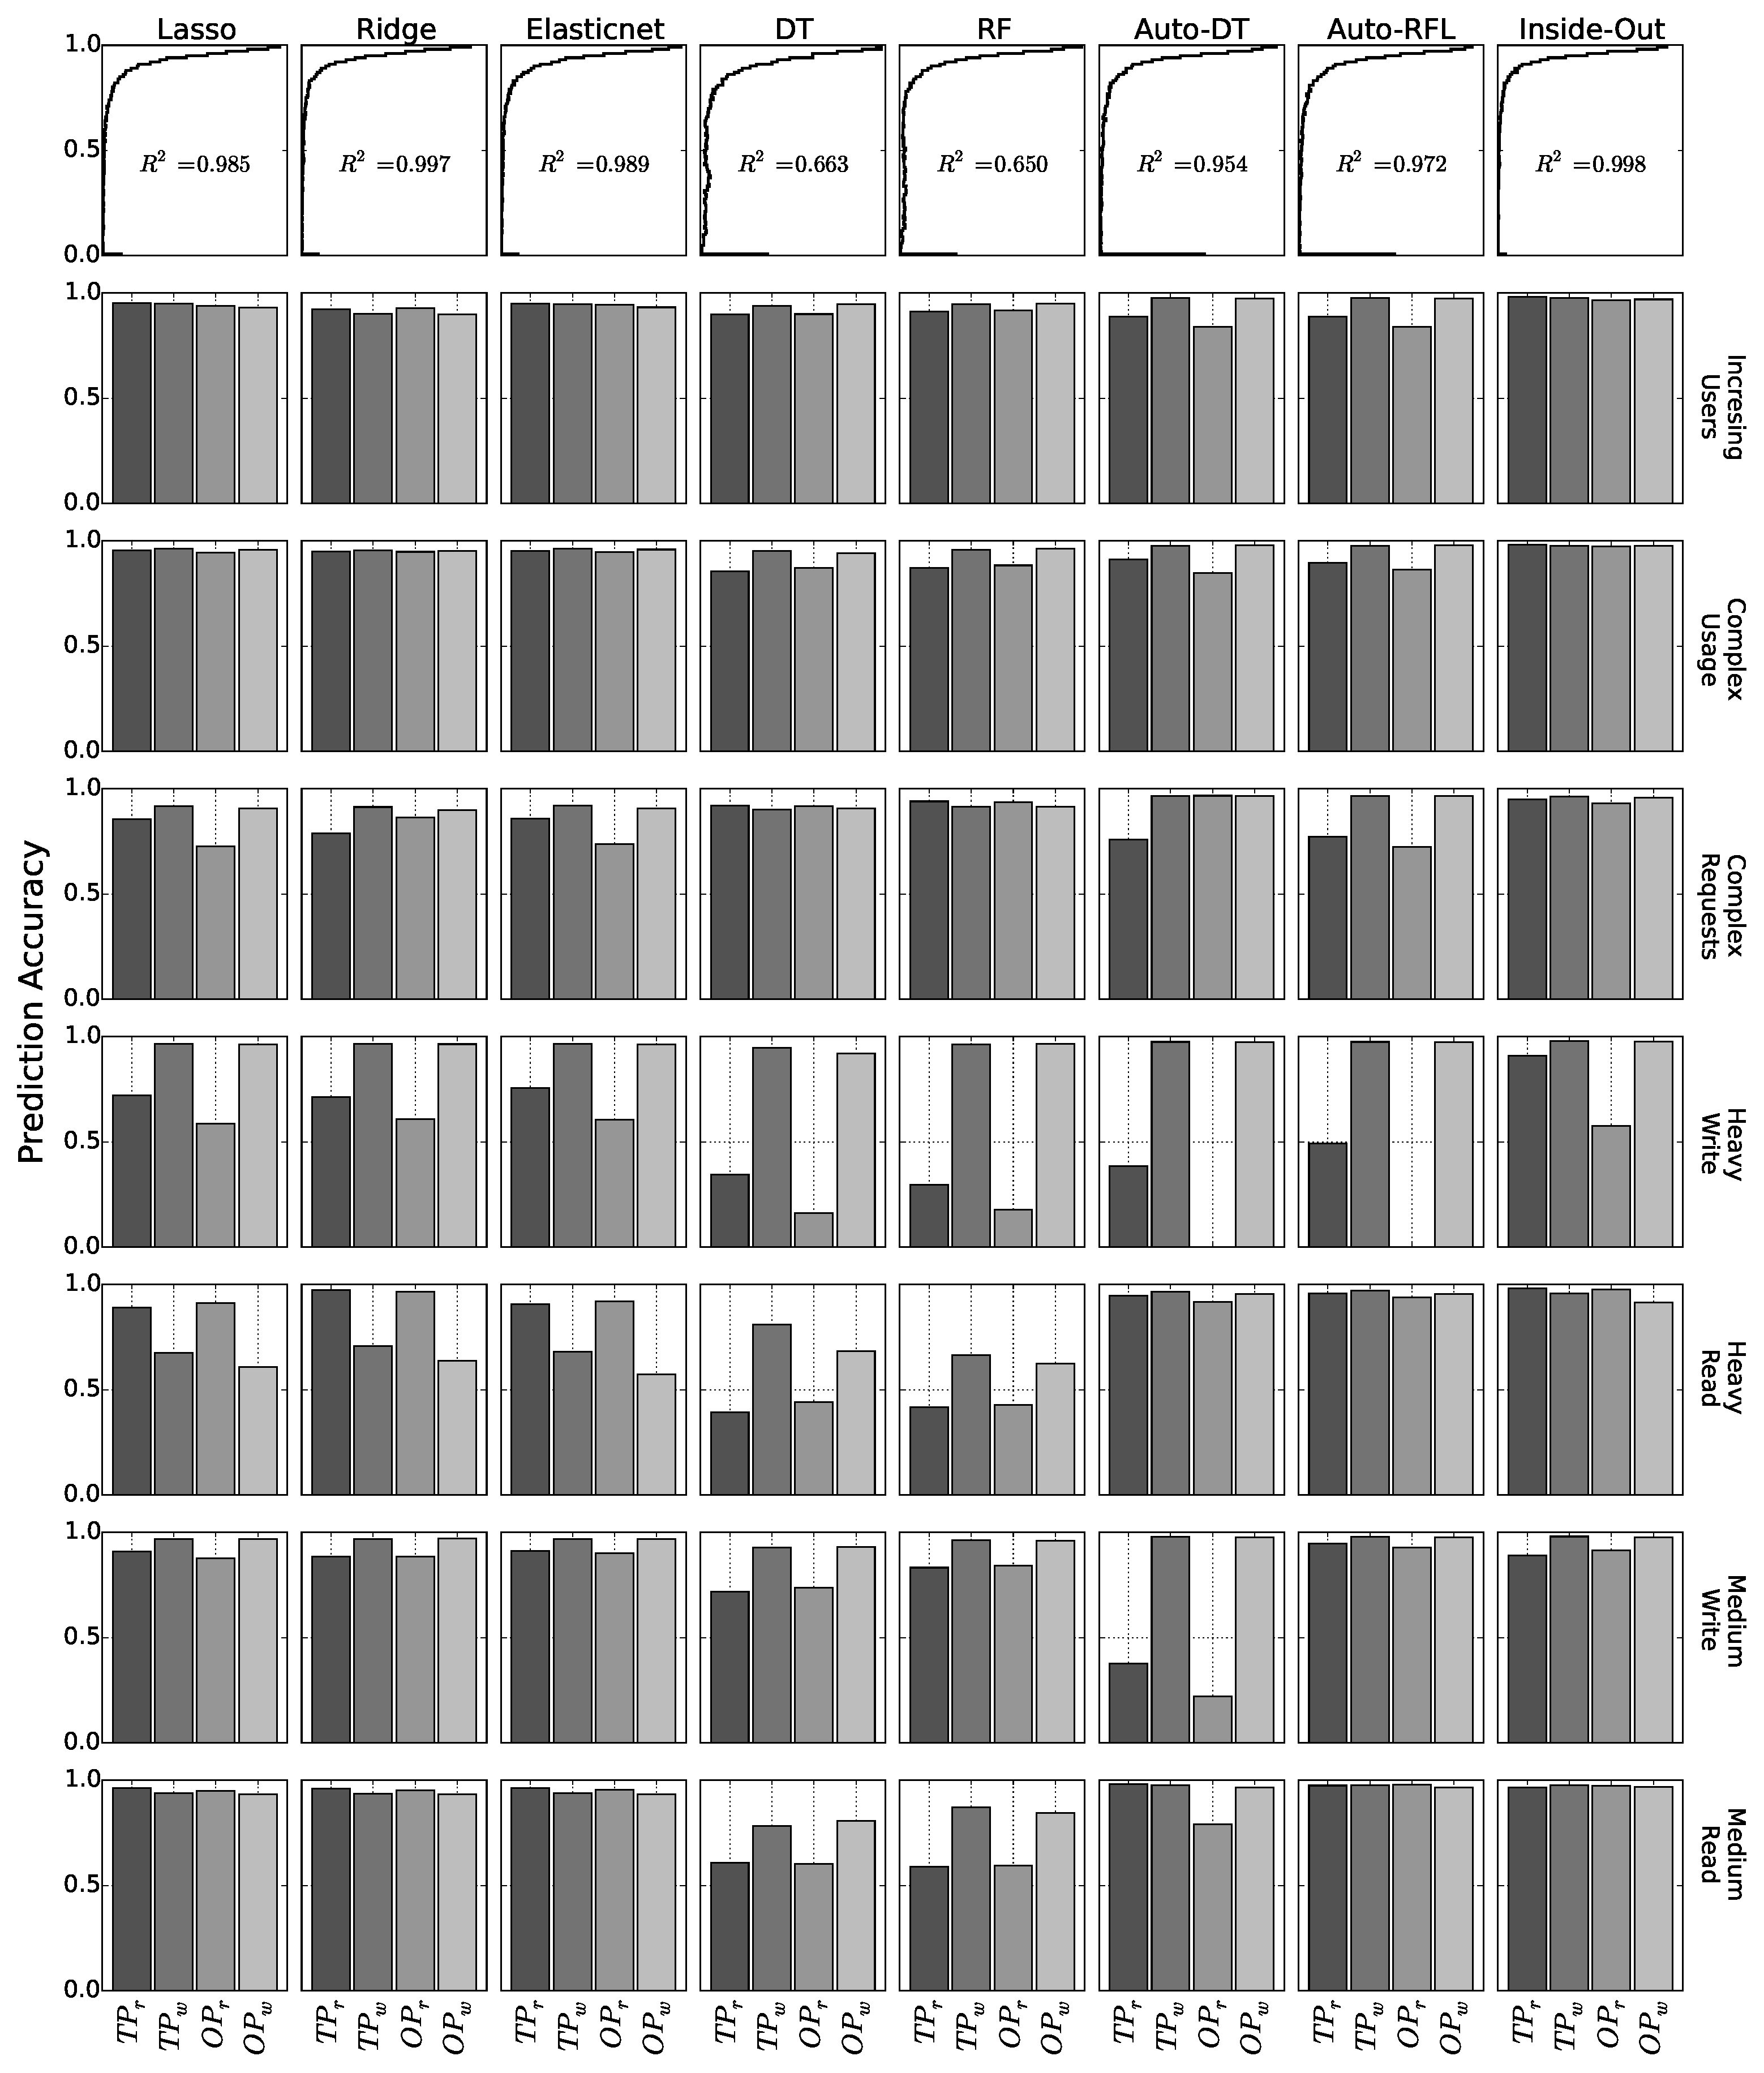
\includegraphics[width=0.9\textwidth]{Chapter-InsideOut/figures/unseen_workload_all_new.eps}
    \caption{Analysis of performance models with diverse workloads. Each bar is the average prediction accuracy. The top row is the probability density function of prediction accuracy for each performance model.}
    \label{fig:changing_workload}
\end{figure}

%\hfill\break

An SDS application needs to handle various request volumes, object/file sizes and different ratios of read/write workloads.
%In practice, it is difficult to obtain a training dataset that includes all access patterns.
First we examine whether Inside-Out can achieve accurate and consistent predictions when workload changes.


\paragraph*{Changing user behavior}
%\textbf{Changing user behavior.}

We increase the number of concurrent clients to stress the Ceph cluster.
%We push the Ceph cluster to a certain limit by increasing the parallelism of clients.
The \emph{\MakeLowercase{\scenarioMU}} scenario changes the number of COSBench clients and the \emph{\MakeLowercase{\scenarioCUB}} scenario increases the worker threads of each client.
As shown in \myfigure{\ref{fig:changing_workload}}, all prediction models perform well. The linear regression technique performs slightly better than the tree-based learning.
The linearly increasing load is well captured by linear models because of proportional change in low-level metrics.
When we switch to the \emph{\MakeLowercase{\scenarioCRB}} scenario, the variable request size slightly changes the behavior of Ceph, affecting prefetching and caching. 
We observe that the linear regression methods (Lasso, Ridge and Elastic Net) show drops in accuracy, e.g. 20\% in the $OP_r$ case; however, Inside-Out 
maintains good accuracy. 
The tree-based learning shows comparable predictions (5-10\% lower) with Inside-Out in these settings.



%\textbf{Complex request behavior.}
%Next, we change the workload from a constant IO request size to variable size.
%In this case, Inside-Out slightly improves the prediction accuracy over Lasso, %and outperforms the three linear models.
%Auto-DT and Auto-RFL show inconsistent prediction result with about 15\% %degradation of accuracy, comparing with the best case.
%One possible expalantion is that some important features filtered by DT and RF 
%are removed.
%Lasso and Elastic Net encounters accuracy drop in the read IOPS prediction


\paragraph*{Varying I/O pattern}

%The workload is a strong performance factor to a storage system \cite{Noorshams2013}.
%The read performance, for example, is affected by the amount of concurrent read or write operations.
Next, we consider workloads with different ratios of read to write operations.
\myfigure{\ref{fig:changing_workload}} shows that varying workload poses a big challenge to performance models. 
The linear regression methods (Lasso, Ridge and Elastic Net) present better prediction accuracy than tree-based models (DT, RL).
In addition, we observe that several models make poor predictions of $TP_r$ and $TP_r$.
The reason is that read behavior is largely affected by \textit{cache}, and large read variance contributes to low prediction accuracy.
Inside-Out performs consistently well, whereas the three linear regression techniques show accuracy drops.
One exception is the $OP_r$ prediction in the \textit{write-intensive} scenario even though $TP_r$ prediction is accurate.
As we will show later in Section~\ref{sec:online_learning}, \emph{over- and under-predictions} cause such behavior. 
The self-learning property of Inside-Out improves its prediction accuracy as it keeps learning the new storage behavior.


\begin{figure}
    \centering
    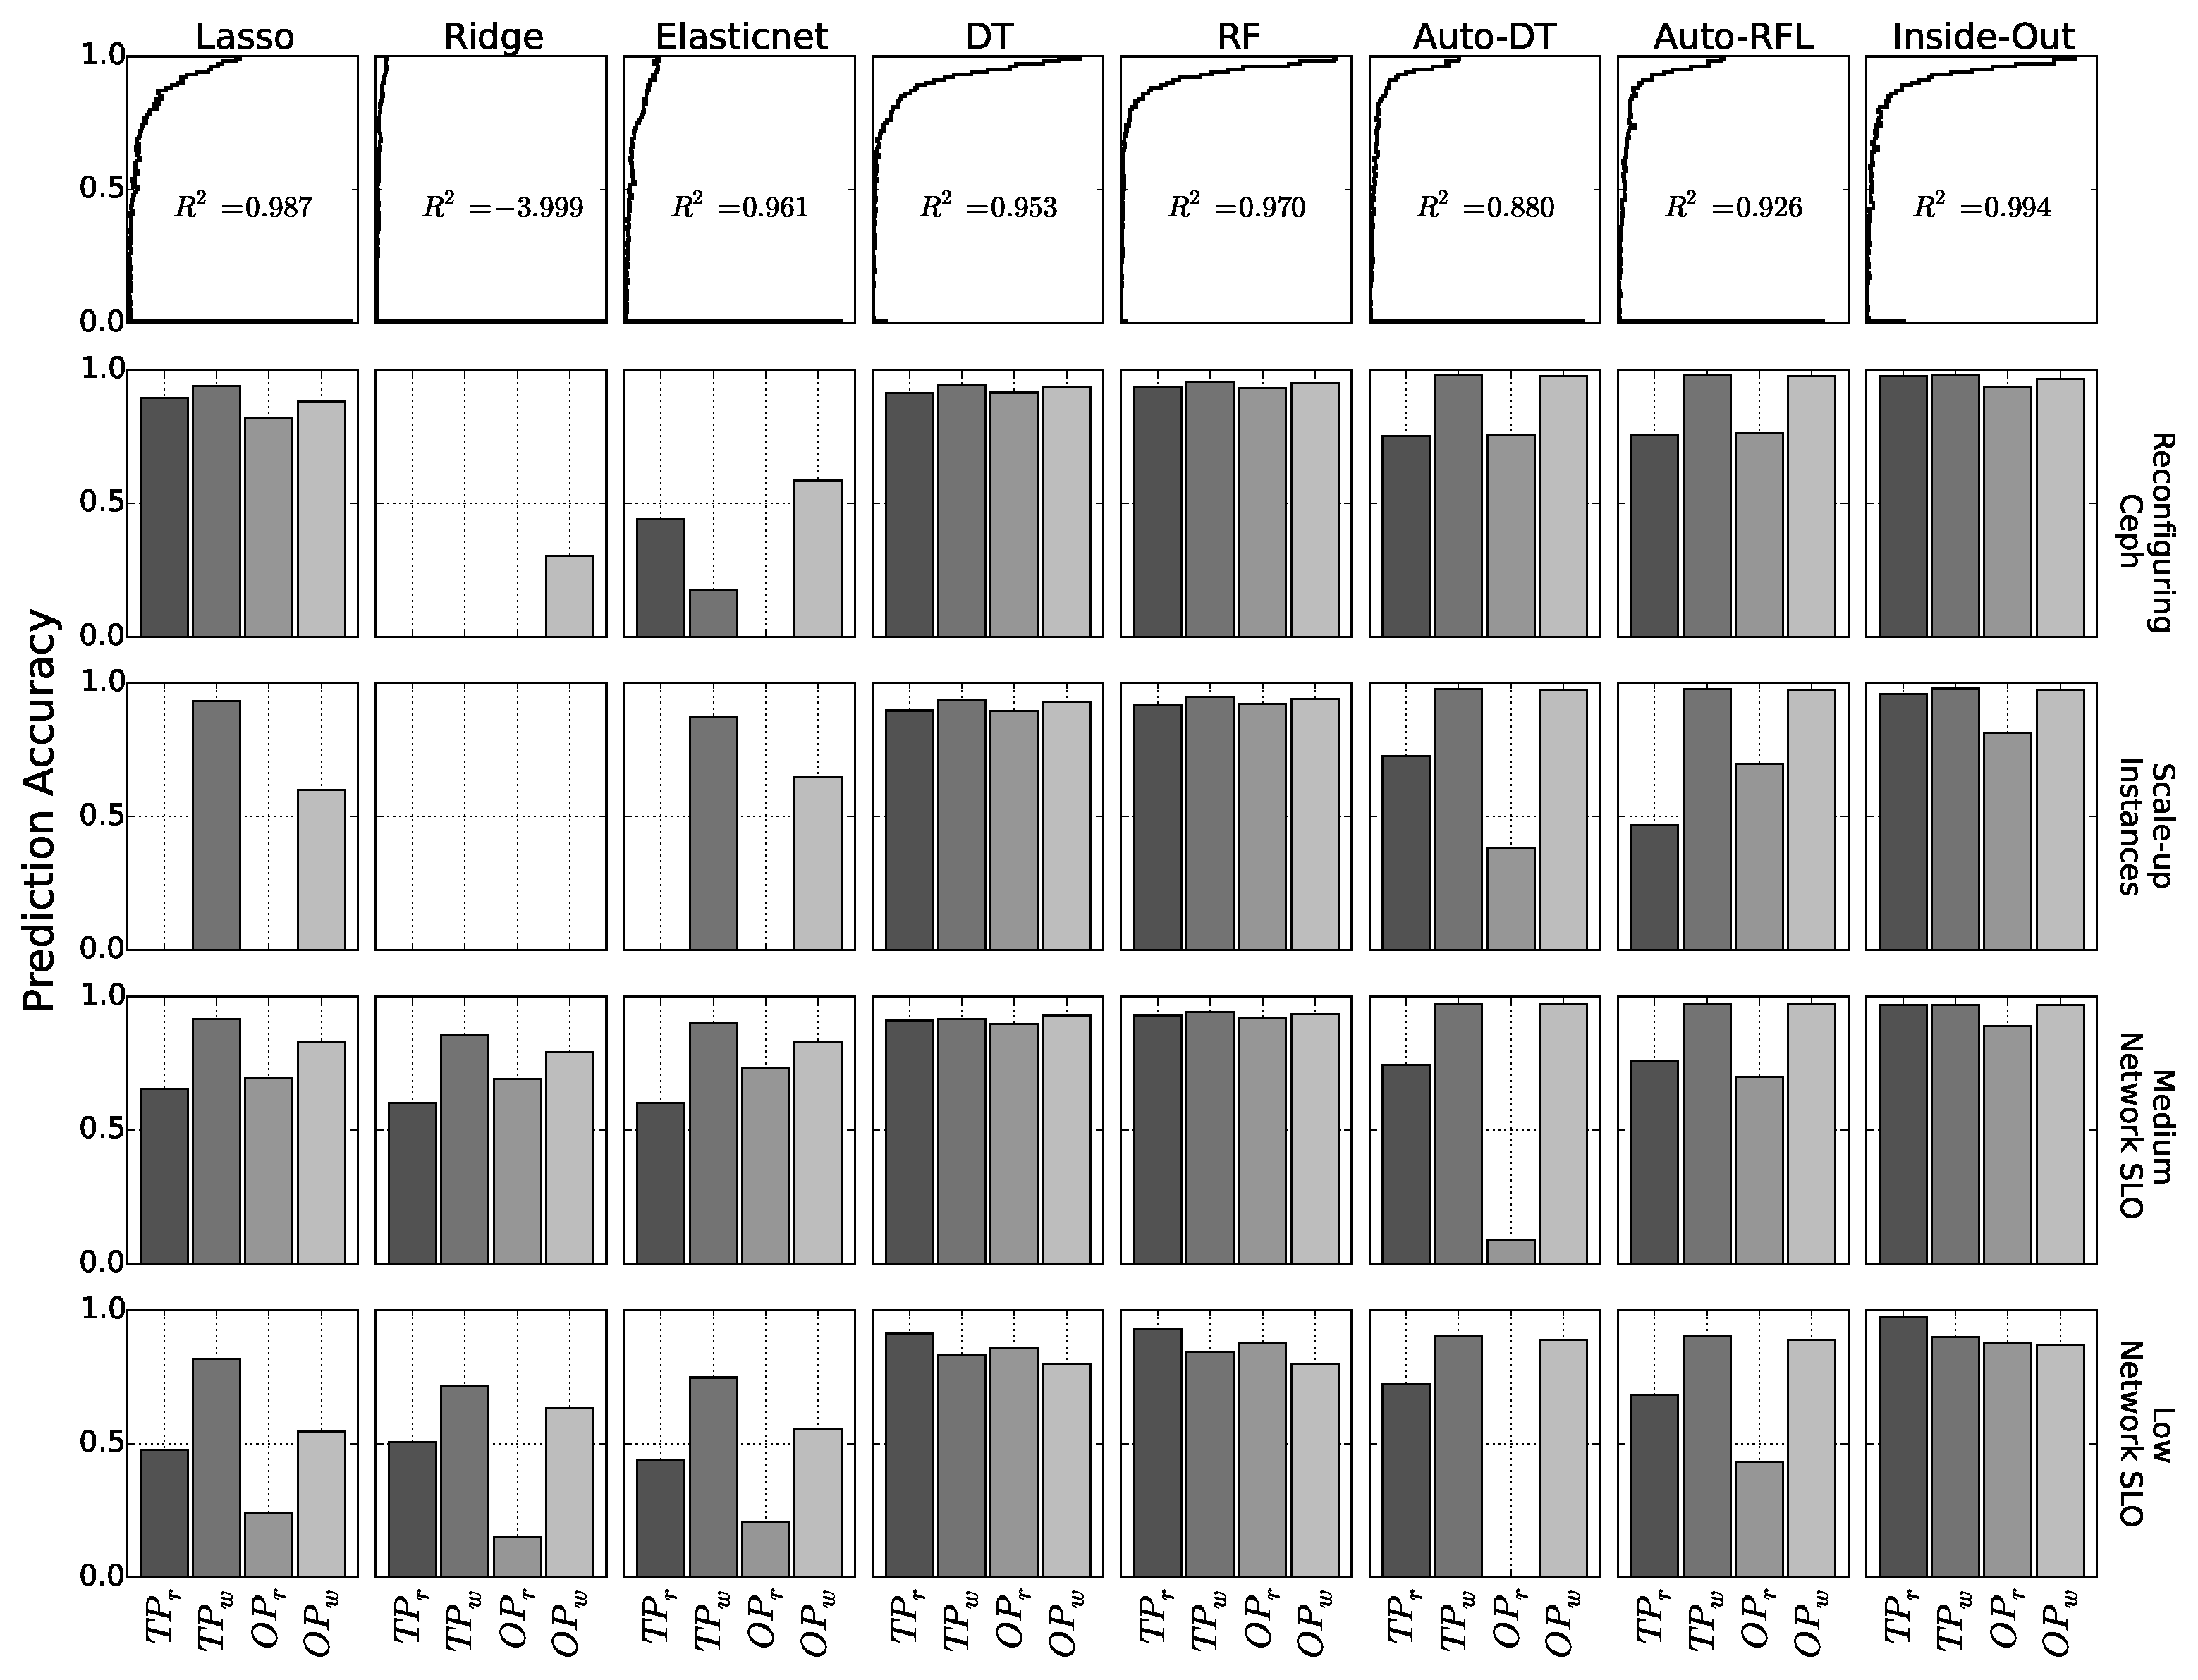
\includegraphics[width=0.9\textwidth]{Chapter-InsideOut/figures/unseen_configuration_all_new.eps}
    \caption{Comparison of performance models when the storage service is reconfigured: Ceph, VMs and network SLOs}
    \label{fig:reconfiguring_storage}
\end{figure}


\paragraph*{Summary}
The linear regression models achieve high prediction accuracy, great goodness-of-fit ($>0.98$) and consistency in prediction 
for many instances (see the distribution of prediction accuracy in \myfigure{\ref{fig:changing_workload}}), but they 
are not consistent across all prediction scenarios.
Inside-Out achieves good prediction accuracy across all cases consistently because the two-level approach 
filters out many irrelevant features in the first step, thereby presenting a smaller relevant feature space to the second step. 
The tree-based learning methods (DT and RF) do not show consistent prediction across all scenarios.
Auto-DT and Auto-RFL, which use DT and RF as the filter algorithms, are not as consistent as Inside-Out.

\vspace{1ex}

%\subsubsection{Reconfiguring Storage}
\subsubsection{Can Inside-Out handle different system configurations?}
\label{sec:unseen_configuration}

We study whether low-level metrics can capture the storage behavior when it is reconfigured by tenants. The results are reported in \myfigure{\ref{fig:reconfiguring_storage}}.


\textbf{Reconfiguring Ceph.}
The first change is to add one extra Ceph monitor daemon. %\chin{which increases the capability to handle a large number of clients.}
Ridge and Elastic Net fail to generate consistent predictions, but Lasso is able to achieve around 80\% to 90\% prediction accuracy.
DT, RF and Inside-Out have very close prediction accuracies, but Auto-DRL and Auto-RFL perform slightly worse in predicting $TP_r$ and $OP_r$.

\textbf{Scale-up instances.}
Increasing CPU and memory allocation to Ceph VM instances improves Ceph's ability to handle more requests.
In this test, we change the instance type from m1.small (1 vCPU, 2GB memory) to m1.medium (2 vCPUs, 4GB memory).
The linear models are unable to predict $TP_r$ and $OP_r$, but Inside-Out's two-level learning performs well by avoiding the overfitting problem. 

\textbf{Network SLOs.}
Here we consider the case where the amount of network bandwidth allocated to Ceph VMs is limited. 
We use Linux network throttling tool \textit{tc} to limit network bandwidth at 500 Mbps and 250 Mbps for medium and low bandwidth SLOs, respectively.
We observe that linear models without the two-level method do not show comparable prediction accuracy across both throughput and IOPS predictions.
The tree-based learning models, on the other hand, achieve 80\% to 90\% accuracy, comparable to Inside-Out.


\textbf{Summary.}
Tree-based learning (DT, RF) models demonstrate promising prediction in terms of prediction accuracy and consistency.
Lasso, Ridge and Elastic Net show inconsistent behavior in the above four scenarios.
Inside-Out, on the other hand, provides consistent predictions and improves Lasso, from 23.9\% to 87.6\% in the extreme case.


\begin{figure}
    \centering
    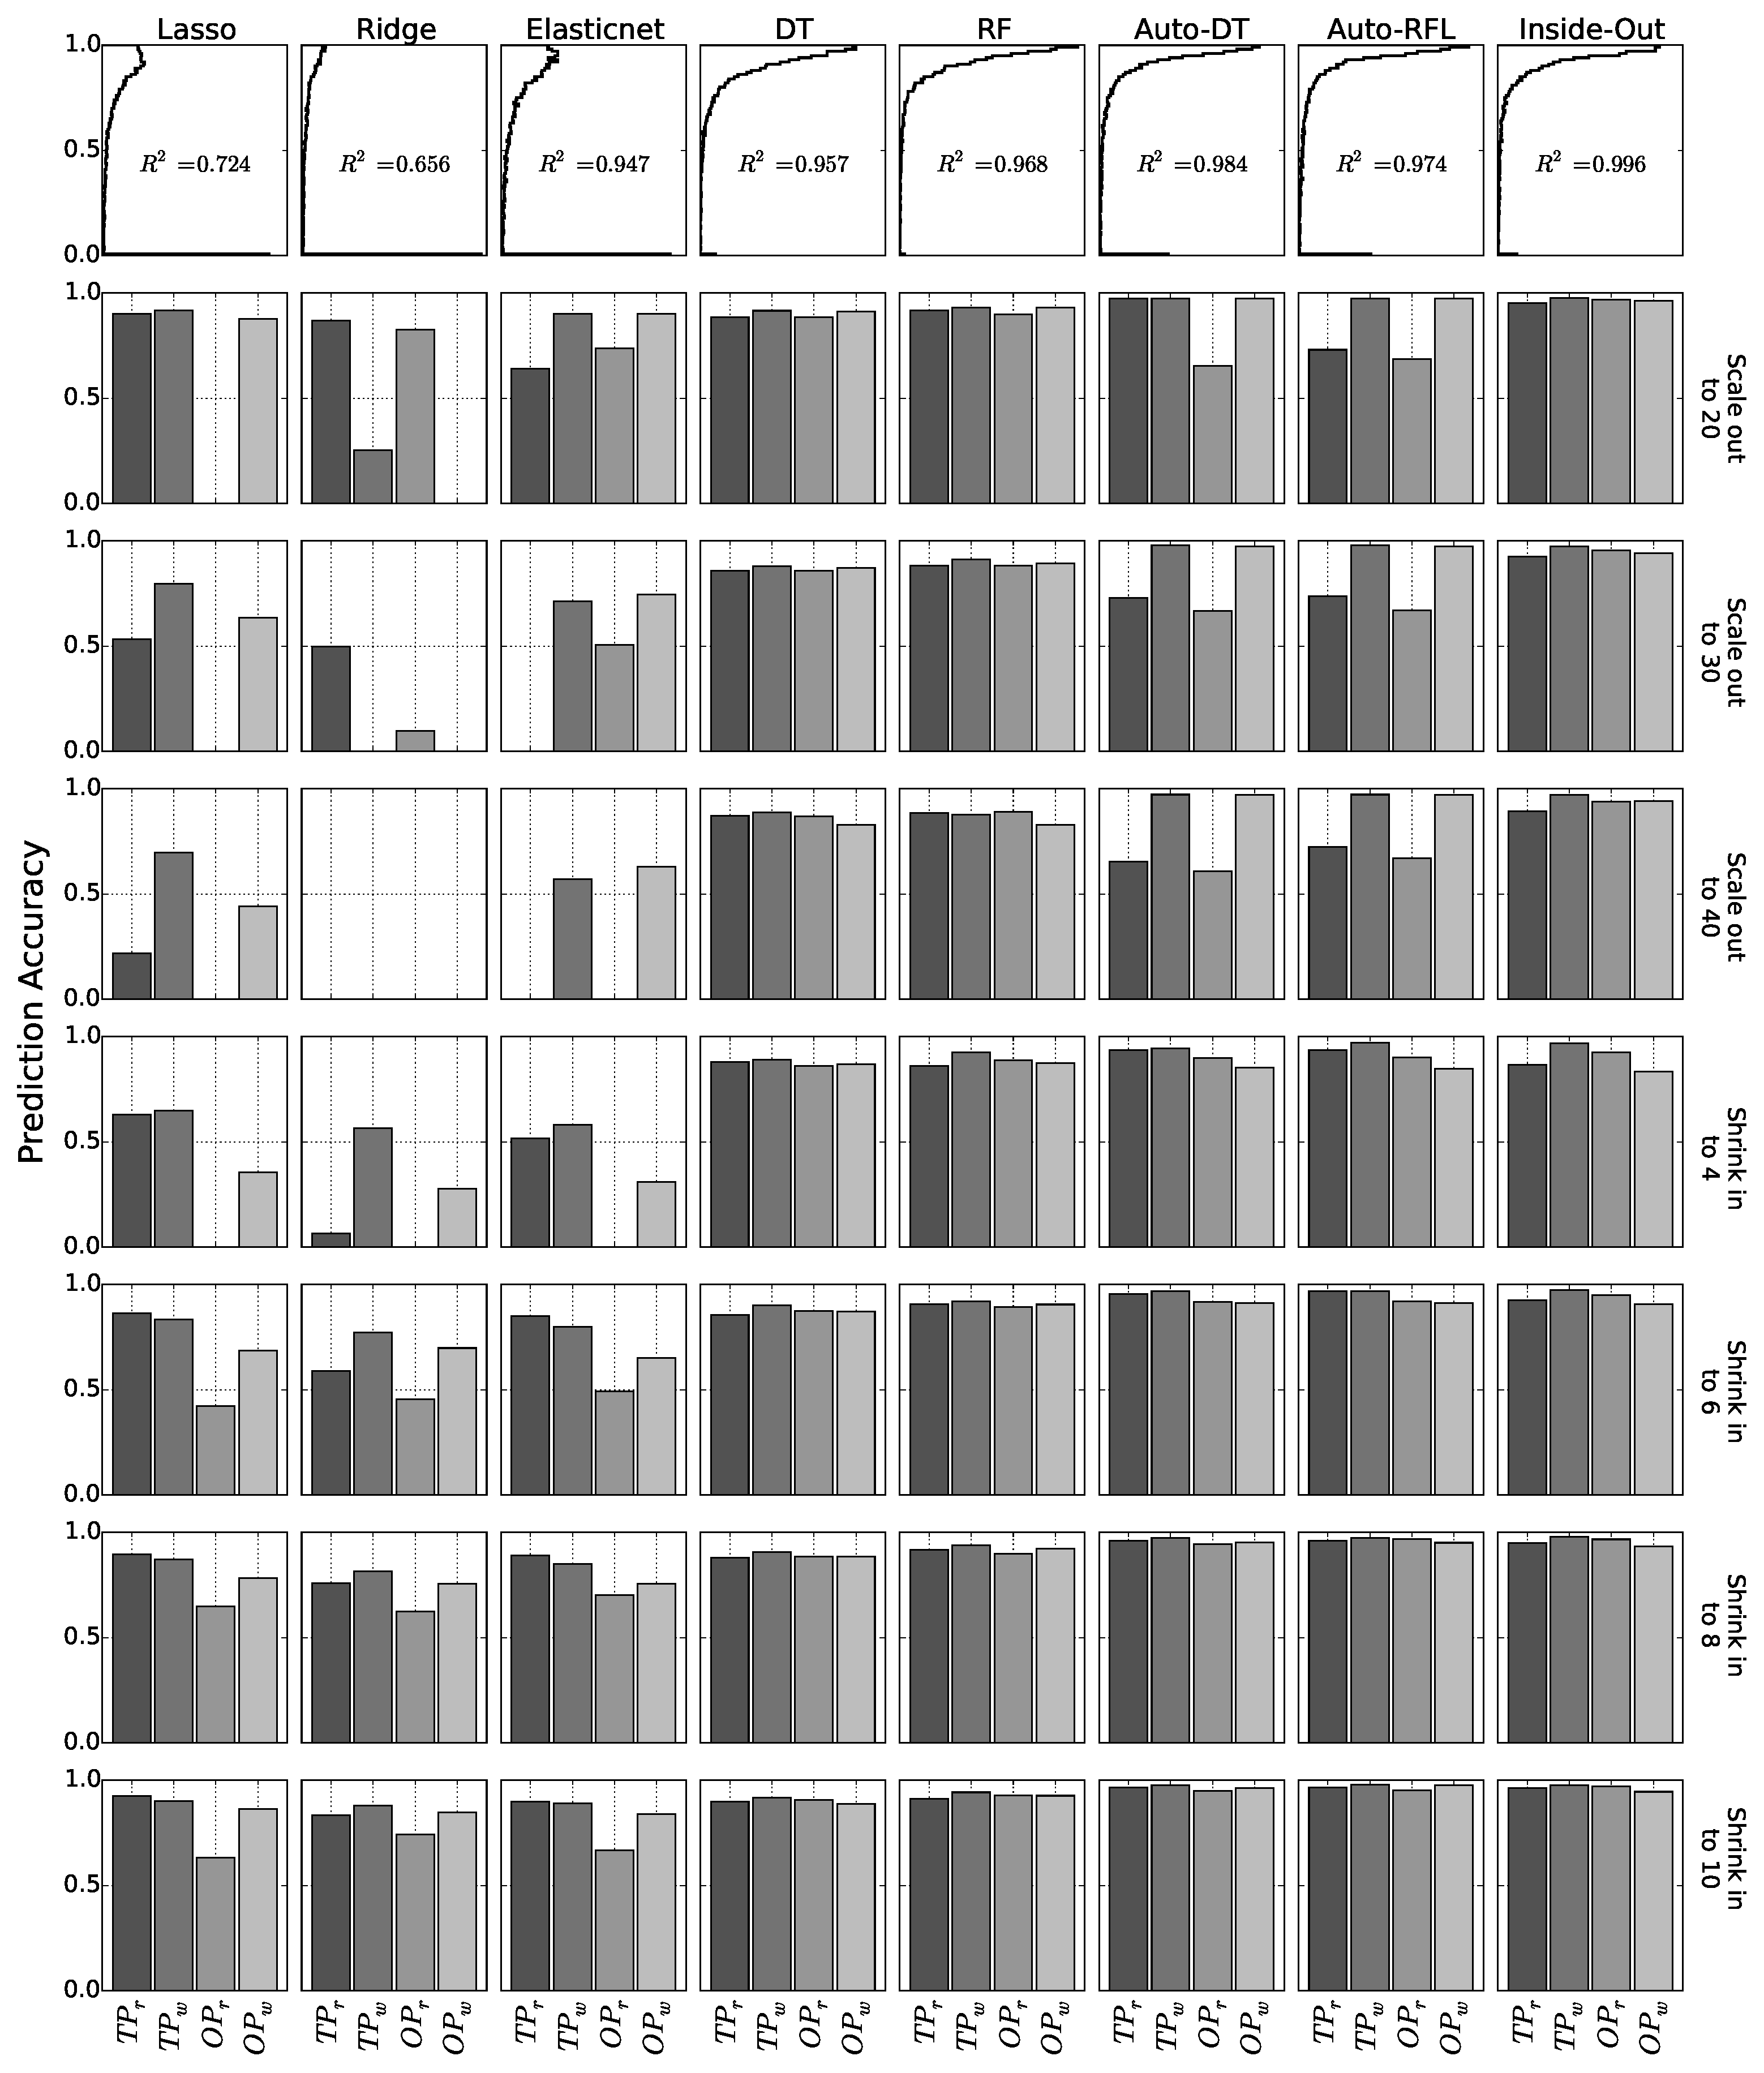
\includegraphics[width=0.9\textwidth]{Chapter-InsideOut/figures/unseen_scale_all_new.eps}
    \caption{Comparison of model performance in the on-demand scaling scenario. In the scale-out scenario, a performance model trained with 10 Ceph nodes is used to predict the performance of Ceph cluster with 20, 30 and 40 nodes.}
    \label{fig:elasticity}
\end{figure}


\subsection{Prediction Performance in a Multi-tenant Cloud}

This section examines the modeling performance of Inside-Out.
We first evaluate whether Inside-Out is able to extrapolate
performance of a larger Ceph cluster. 
Next, we evaluate how Inside-Out performs
when systems are subject to performance interference.

\subsubsection{Elastic Storage (On-demand Scaling)}
\label{sec:scaleout_prediction}

A storage service needs to grow or shrink its capacity on demand.
We evaluate Inside-Out's ability to capture the storage behavior at different system scales.
As shown in \myfigure{\ref{fig:elasticity}}, we use training data collected from 
4, 6, 8, and 10 nodes, and then predict the performance of 20, 30, and 40 nodes.
We also evaluate prediction accuracy in the \emph{shrink-in} scenario.
For both read and write throughput predictions, the linear models exhibit high variance.
In the $OP_r$ and $OP_w$ cases, the prediction results are not even comparable to the other methods.
Inside-Out, on the other hand, helps mitigate this issue, and achieves more than 90\% accuracy.
With increasing sizes of the storage, the prediction accuracy decreases because the prediction target 
becomes increasingly different from the training data.
Running a benchmark test against a very large system is time-consuming.
Here we demonstrate that Inside-Out can predict performance for systems that are 
four times larger than the system for which training data was collected.
%Due to resource limitations, we cannot show the upper bound of the largest system size that we can predict.
%However, we believe the upper bound can increase as the performance model keeps learning the system behavior.

\begin{figure}
    \centering
    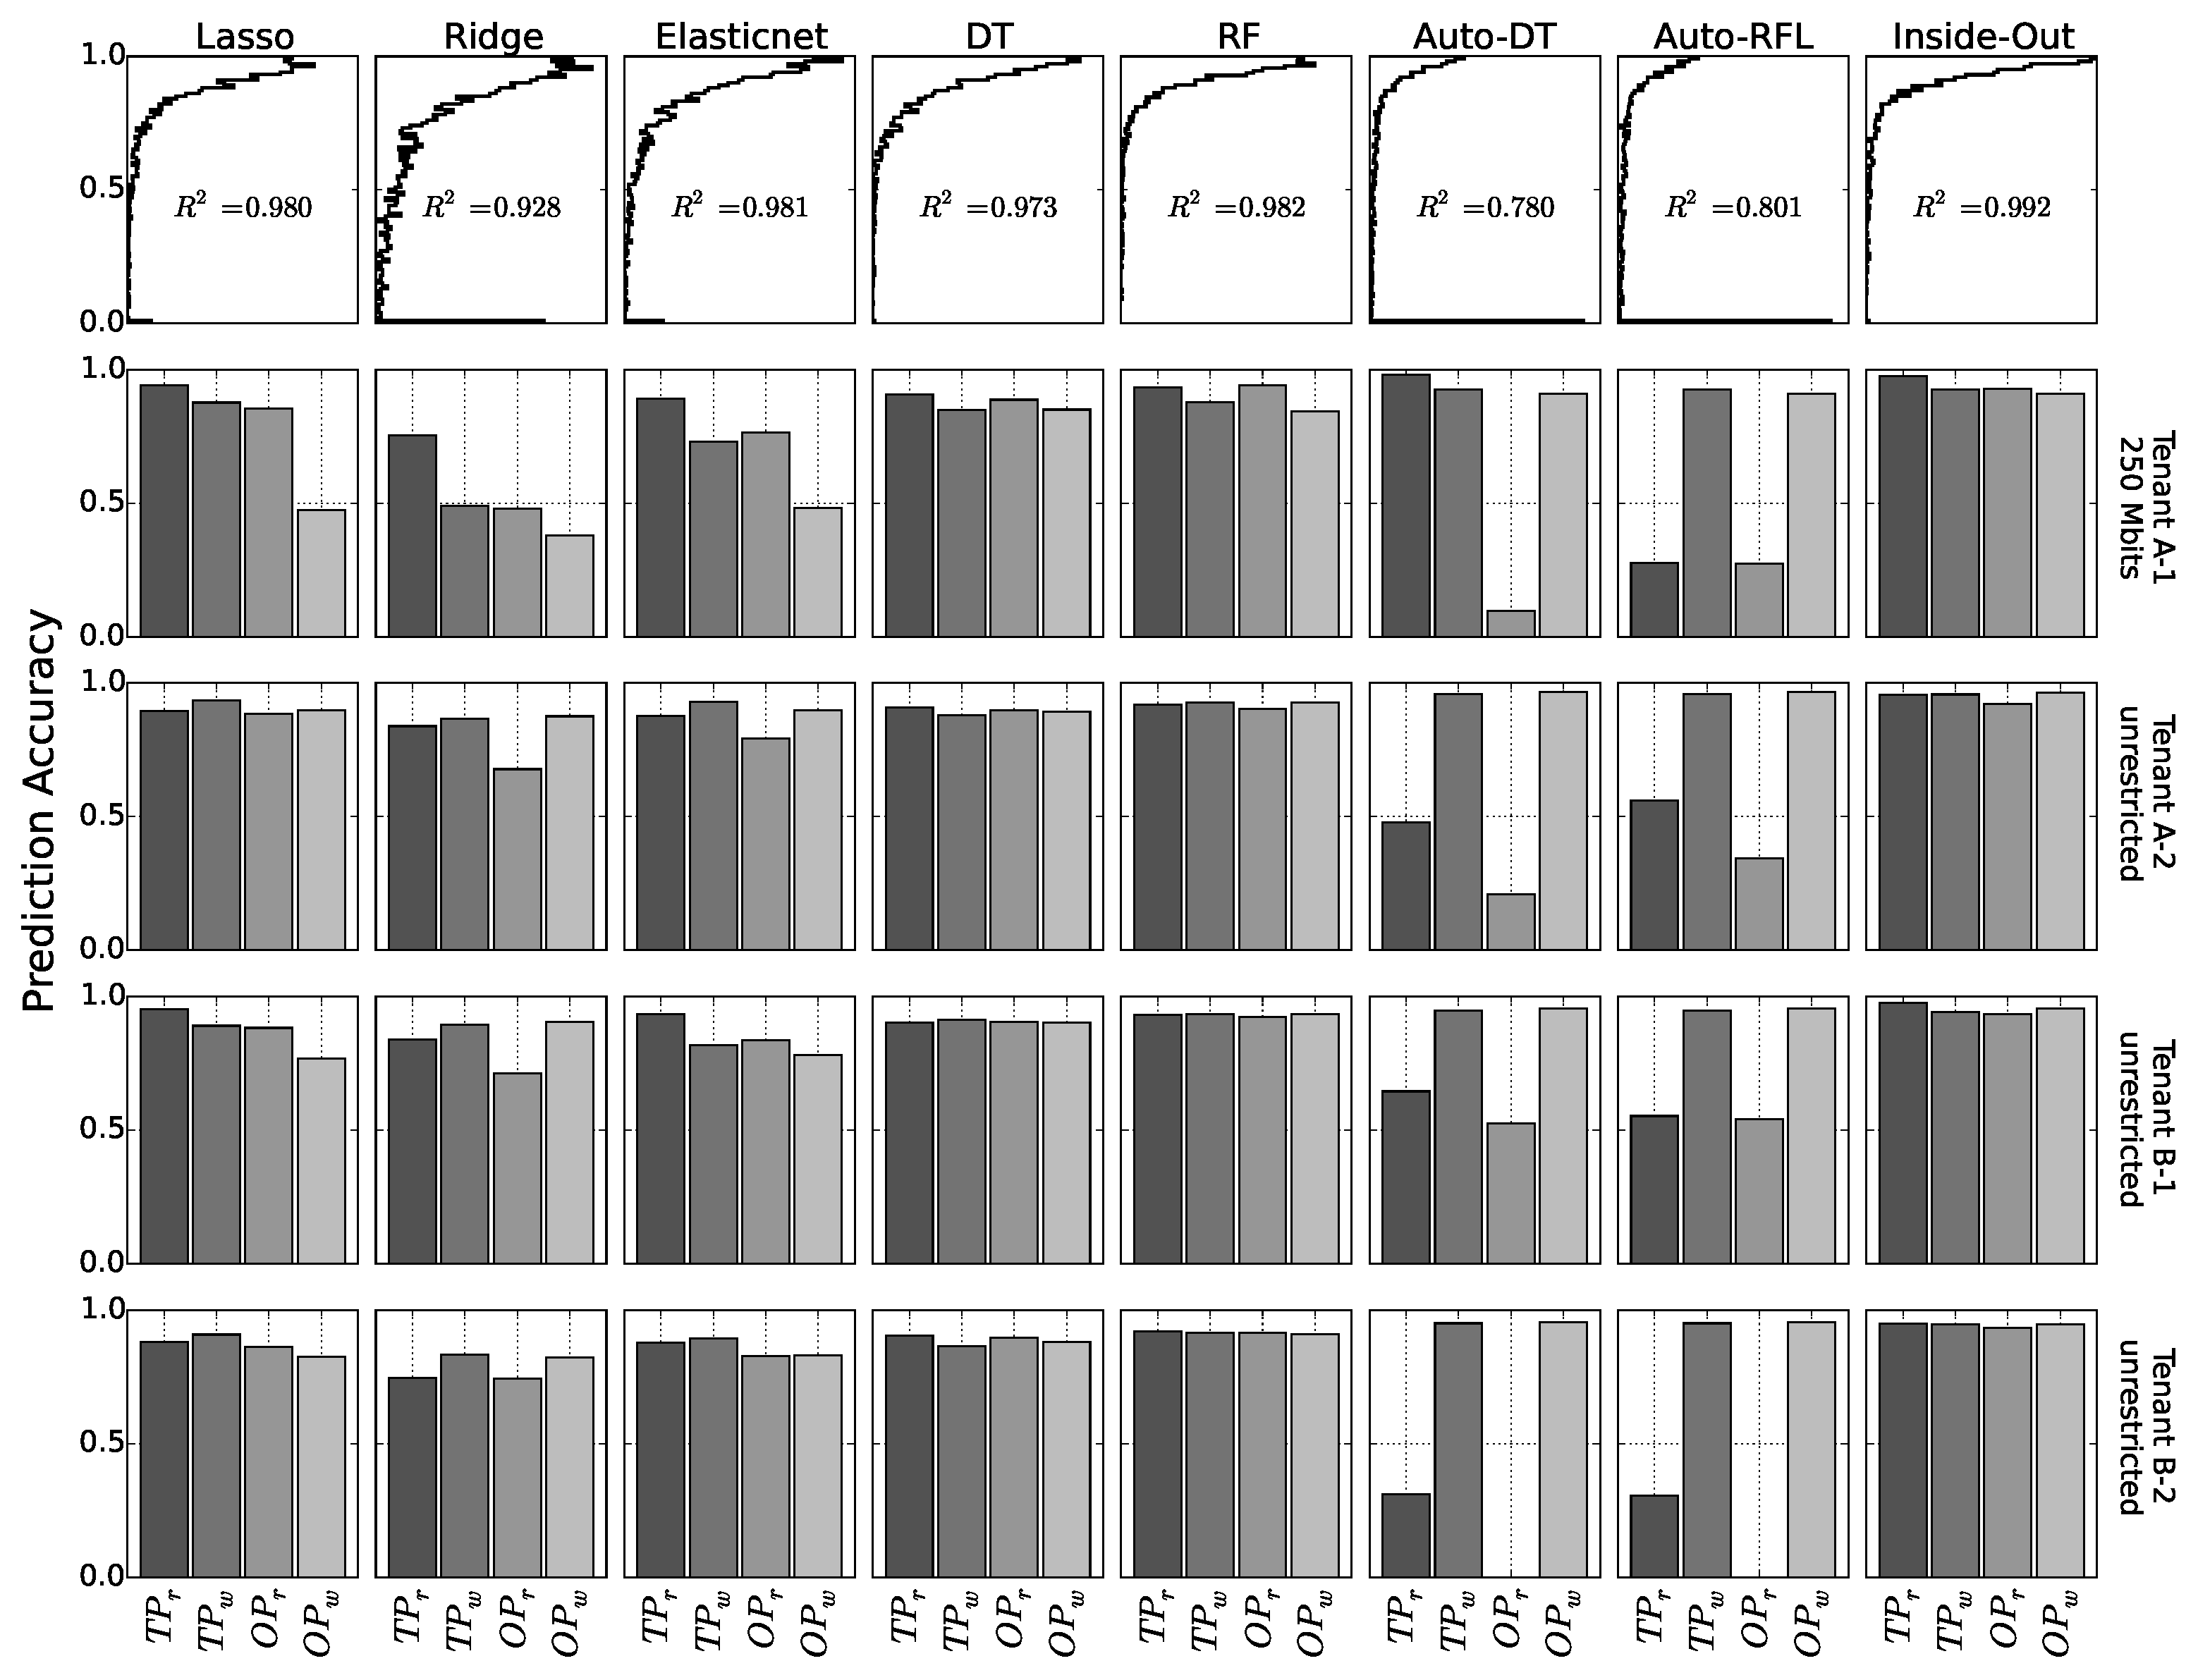
\includegraphics[width=0.9\textwidth]{Chapter-InsideOut/figures/multi_tenancy_all_new.eps}
    \caption{Prediction accuracy in a multi-tenancy scenario. Tenant A-1 is co-located with Tenant B-2. Tenant A-1 is throttled at 250Mbps. Tenant B-1 and B-2 are co-located without any traffic throttling.}
    \label{fig:multi_tenancy}
\end{figure}


\begin{figure*}
    \centering
    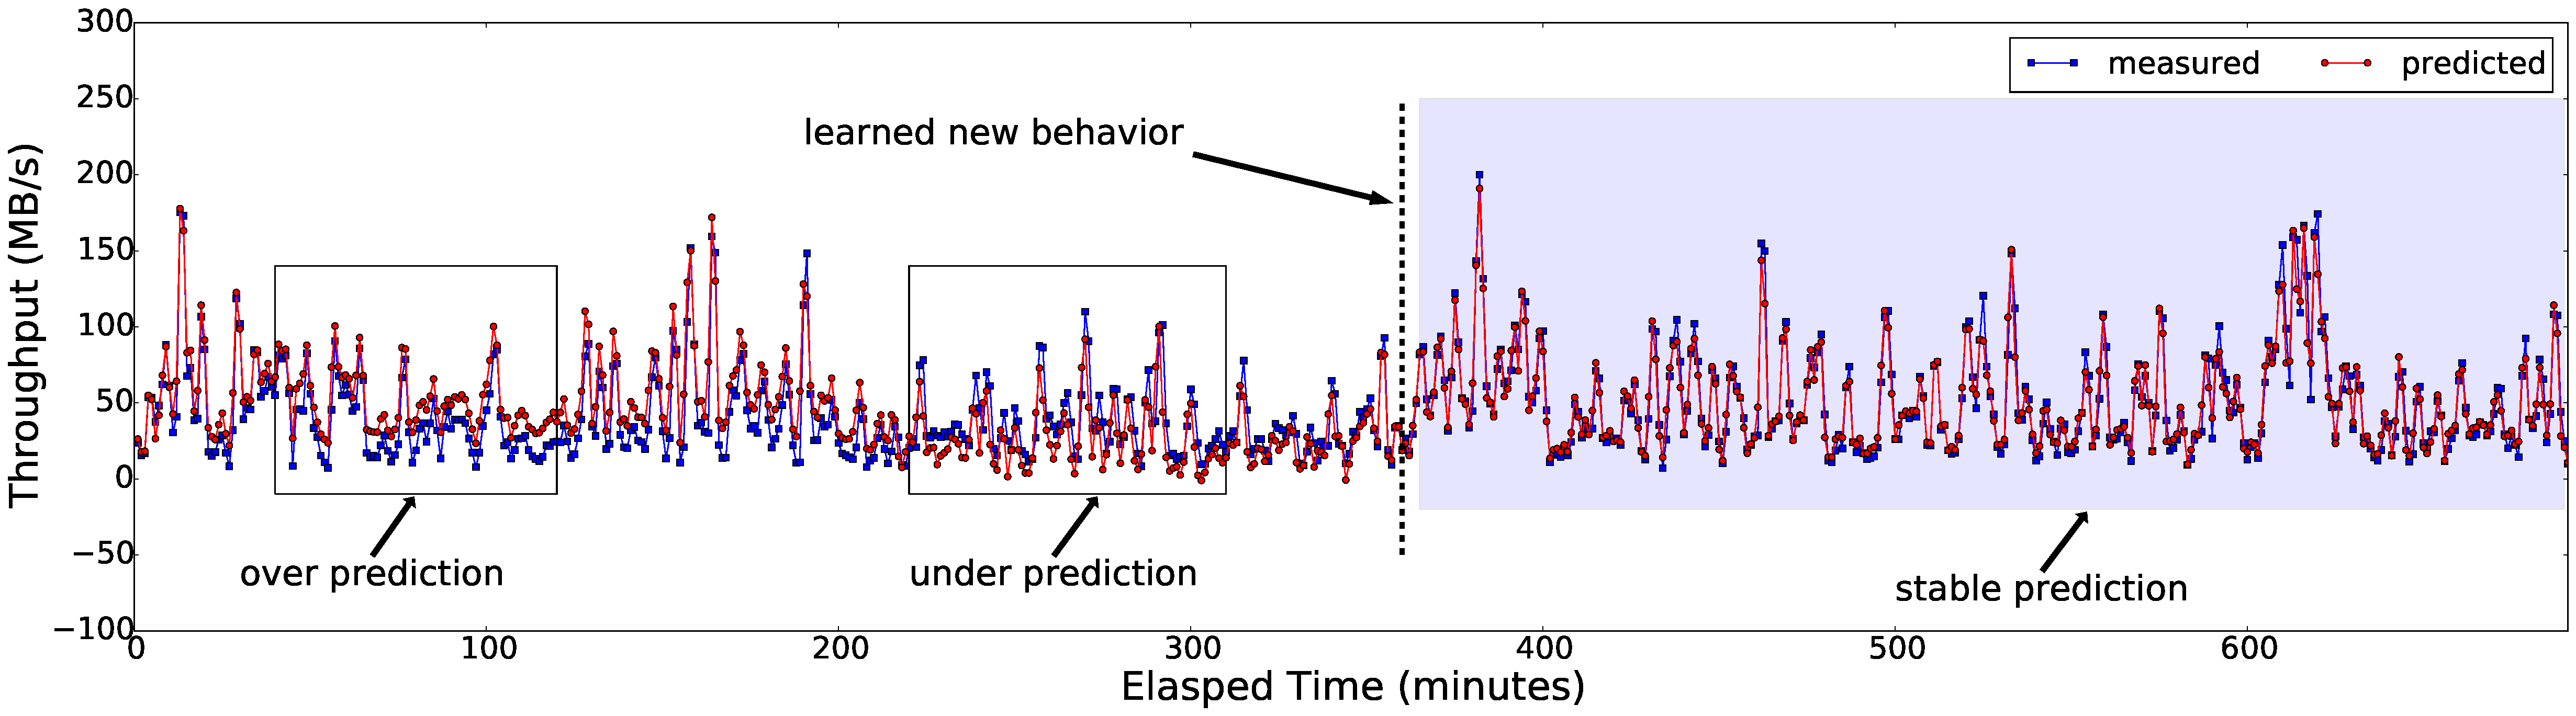
\includegraphics[width=0.9\textwidth]{Chapter-InsideOut/figures/real-world_tp_read.pdf}
    \caption{Application of Inside-Out to real time prediction of read throughput on a 10-node Ceph cluster.  Inside-Out starts from a simple prediction model trained by our collected benchmarking data.  Inside-Out keeps learning the storage behavior while improving prediction accuracy over time.}
    \label{fig:real_workload}
\end{figure*}


\subsubsection{Multi-Tenancy}
 
Next we evaluate Inside-Out's ability to adapt to performance interference among storage tenants.
We consider two cases for this evaluation. 
Each tenant runs a Ceph cluster with 10 OSDs separately, but tenants share the same 10 physical machines.
In the first case, we restrict the bandwidth of only the first tenant at 250Mbps.
%Two tenants compete for resources and \chin{\textbf{Tenant A-1}} has lower bandwidth SLO.
In the second case, we run two concurrent Ceph clusters but without network throttling.
\myfigure{\ref{fig:multi_tenancy}} shows that most prediction models are able to achieve more than 80\% accuracy.
The linear models like Ridge and Elasticnet yield lower prediction accuracies in some cases; however, Inside-Out performs well consistently.
Performance interference is challenging for a performance model designed for an isolated environment.
This evaluation demonstrates that the low-level performance metrics are good proxies for measuring
the end-to-end storage performance, even in a shared SDS environment.
%These metrics are able to reflect the behavior changes in the storage system.

%low-level performance feature selection approach is effective in capturing end-to-end performance, even under high storage interference.
%This property is important to SDS because it can help guarantee reliable end-to-end performance in a shared SDS environment.



\begin{comment}
\begin{figure*}
    \centering
    \includegraphics[width=0.9\textwidth]{figures/synthetic.eps}
    \caption{An online prediction scenario about six-hour long workload.  This synthetic workload is composed of 360 stages and each stage uniformly selects parameters such as workload types, request sizes and the number of clients.  The average stage duration is 60 seconds with standard deviation 20 seconds.}
\end{figure*}
\end{comment}

\begin{comment}
\begin{figure*}
    \centering
    \begin{subfigure}[b]{0.45\textwidth}
        \includegraphics[width=\textwidth]{figures/synthetic_read.eps}
        \caption{Read Throughput}
        \label{fig:synthetic_read}
    \end{subfigure}
    ~ %add desired spacing between images, e. g. ~, \quad, \qquad, \hfill etc.
      %(or a blank line to force the subfigure onto a new line)
    \begin{subfigure}[b]{0.45\textwidth}
        \includegraphics[width=\textwidth]{figures/synthetic_write.eps}
        \caption{Write Throughput}
        \label{fig:synthetic_write}
    \end{subfigure}
    \caption{An online prediction scenario about six-hour long workload.  This synthetic workload is composed of 360 stages and each stage uniformly selects parameters such as workload types, request sizes and the number of clients.  The average stage duration is 60 seconds with standard deviation 20 seconds.}
    \label{fig:synthetic_workload}
\end{figure*}
\end{comment}

%\subsection{Synthetic Workload}
\subsection{Online Self-Learning}
\label{sec:online_learning}

%Our goal is to apply Inside-Out to an online system so that SDS providers can guarantee the performance of a storage service hosted on their SDS platform.
%To evaluate this potential, 
Next, we create several synthetic workloads with mixed read/write ratios.
This synthetic workload spans 12 hours with 720 stages.
Each stage is 60-second long on average, with a standard deviation of 20 seconds.
We run four COSBench virtual machines for benchmarking and up to eight threads per COSBench client, with 10 Ceph OSDs and one monitor daemon.
We use Inside-Out to build an initial performance model with the training dataset described in Section~\ref{sec:dataset}.
\myfigure{\ref{fig:real_workload}} shows the prediction result for read throughput.
We can observe that the generated model can capture the overall trend, but suffers from over and under predictions.
This is because our training dataset is generated from a relatively clean environment, \ie the OS memory is flushed before any benchmarking process.
However, in the online prediction setting, cache is continuously consumed by non-stop client requests, which 
causes the real time storage behavior to be different from the training dataset.
With continuous monitoring of the performance of the storage service, 
we use Inside-Out to generate a new performance model at the sixth hour.
\myfigure{\ref{fig:real_workload}} shows that Inside-Out learns the new storage behavior and therefore, 
the over- and under-prediction issues are greatly mitigated.
%This evaluation demonstrates the potential of Inside-Out when applying it in an online system.
By continuously learning the storage behavior, SDS can accurately capture performance changes and therefore is able to provide reliable storage service.

%the problems due to over- and under-predictions are greatly mitigated.
%This evaluation demonstrates how Inside-Out can be used to continuously learn the storage behavior in an online system.


\begin{figure}
\centering
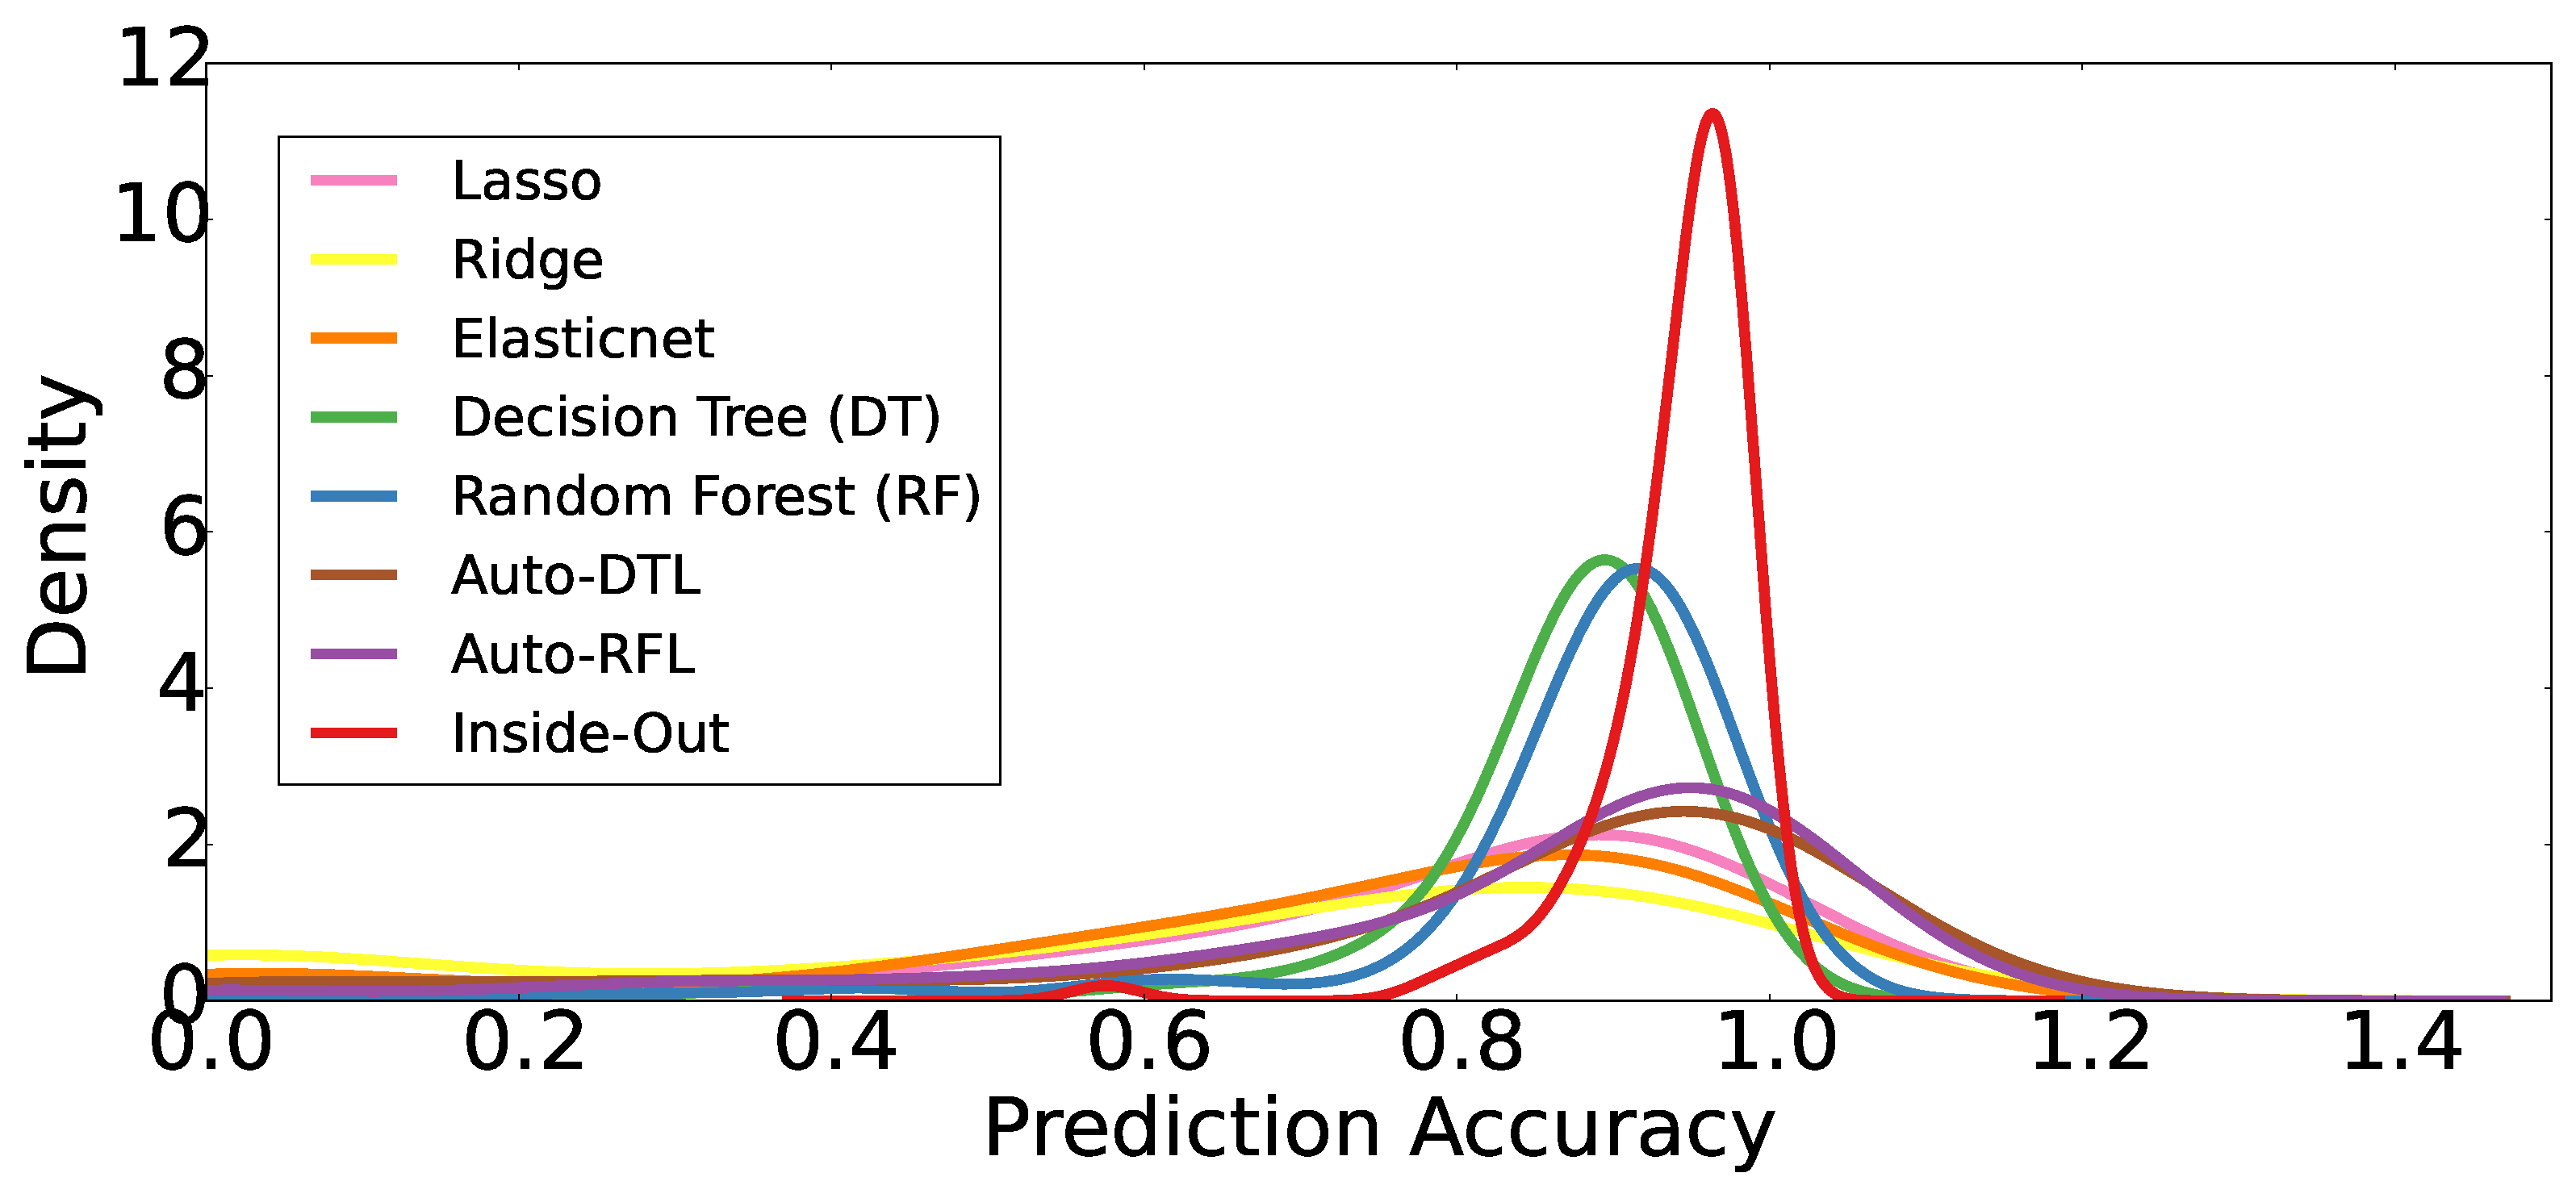
\includegraphics[width=0.9\textwidth, keepaspectratio]{Chapter-InsideOut/figures/aggregate_median.eps}
\caption{Kernel density function of prediction accuracy from \myfigure{\ref{fig:changing_workload}} to \myfigure{\ref{fig:multi_tenancy}}.  Each colored line represents the density function of a modeling approach.  Inside-Out is more consistent and accurate across almost every prediction case.}
\label{fig:aggregate}
\end{figure}


\vspace{1ex}
\subsection{Discussion}
We have shown that low-level performance metrics are useful to predict end-to-end throughput and IOPS.
%We applied Inside-Out to latency prediction and observe large variance and inconsistency.
%\chin{One} possible explanation is insufficient features and high variance in latency.
%The \chin{collected} low-level metrics are related to utilization, and these metrics might not provide enough information to fit a good model for predicting latency.
%Common approaches usually require request-level information \cite{Wang2004}.
%We need to further investigate latency prediction with other alternative generic low-level performance metrics.
Our evaluation has shown that low-level performance metrics are good indicators of end-to-end throughput and IOPS. 
Most existing performance models exhibit an inconsistent prediction behavior in the presence of diverse storage scenarios, 
such as changing workload, storage reconfigurations,
growing/shrinking storage, and multi-tenancy environments.
Our proposed two-level learning method can greatly improve prediction accuracy and yield consistent behavior.
Machine learning provides powerful tools, but they need to be used intelligently to achieve the best prediction accuracy. 
\myfigure{\ref{fig:aggregate}} shows the kernel density function of prediction accuracy across all prediction scenarios.
Inside-Out is a clear winner in terms of accuracy and consistency. 
More importantly, Inside-Out is able to learn new storage behavior, thereby enabling the performance model to adapt to the complex SDS environment.





% %\section{Related Work}
\label{ch4:sec:relatedwork}

Storage performance modeling has been extensively explored in many prior works. 
Three common modeling techniques are analytical, simulation and data-driven approaches \cite{Shriver1998, Kelly2004, Ardagna2014}.
The analytical (mathematical) model requires domain knowledge to manually identify the factors that affect performance\cite{Shriver1998, Kelly2004}.
Kelly et al. use a probability model to predict response time for an enterprise storage array.
Ruemmler et al. found that a disk is too complex to model with analytical methods and designed a disk simulator to characterize storage behavior \cite{Ruemmler1994}.
However, the simulation approach becomes inefficient when searching a large design space \cite{Kelly2004}.


The data-driven or the measurement-based approach
uses measurement data to derive a prediction model. 
Wang et al. \cite{Wang2004} adopt classification-and-regression-tree (CART) to predict the response time of a single disk and a disk array.
The authors propose request-level and workload-level device models for different prediction granularities.
Yin et al. also use the regression tree to predict storage throughput and latency \cite{Yin2006}.
Their work mainly focuses on multiple workloads, and proposes a scalable model, by combining related workload features.
Noorshams et al. extensively analyze four different types of algorithms 
(including linear regression and CART models) and apply to IBM storage servers \cite{Noorshams2013}.
They also propose an optimization technique to search for parameters that can improve prediction accuracy.
Their proposed parameter optimization complements our work for improving prediction accuracy.
To sum up, Inside-Out uses only low-level performance metrics and does not require workload profiles and storage configurations.
Unlike these studies, Inside-Out is primarily designed for diverse storage services that need to be reconfigured frequently to meet users' demand. 


Mesnier et al. \cite{Mesnier2007} propose a novel black-box approach that can describe the performance difference between two storage devices.
It may be possible to borrow this idea and apply it to the unseen configuration scenarios as described in Section \ref{sec:unseen_configuration}.
With this approach, we can study the performance difference between two configurations and create a combined model with better prediction accuracy.
Bodik et al. propose an exploration policy for quick collection of essential data required to train a performance model \cite{Bodik2009}.
This policy can reduce the time required for offline and online model training.


Chen et al. propose SLA decomposition that combines profiling and queuing model to derive resource thresholds for meeting application SLA \cite{Chen2007}.

%SLA decomposition is used to determine the resource threshold that can meet a certain SLO \cite{Chen2007}.
%In \cite{Chen2007}, the authors propose using component profiling to build a queuing network model for predicting end-to-end performance. 
%Our black-box approach does not require domain knowledge.
%Their work focuses on three-tier web applications and our focus is to create accurate performance models for software-defined storage.
%Moreover, we consider more realistic cases such as unseen workload, different configurations, resource interference and varying cluster sizes.
%% to add
%% \cite{Madhyastha2012}

Machine learning has also been applied to performance modeling for virtual machines (VMs).
DeepDive uses the classification technique to detect performance anomaly among VMs \cite{Novakovic2013}.
In \cite{Kundu2010}, the authors apply regression and artificial neural network to model performance of a single VM.
Our work focuses on performance prediction of a distributed storage system that includes multiple software and hardware entities.

% \section{Conclusion}
\label{sec:conclusion}

Ensuring end-to-end performance in software-defined storage (SDS) requires accurate performance models. This chapter presents Inside-Out, a tool that provides reliable and consistent prediction of end-to-end performance of distributed storage systems using low-level system metrics. Our evaluation indicates that Inside-Out is able to generate accurate prediction models even when the storage environment differs significantly from the training phase. Inside-Out is generic in nature because it does not use application or protocol specific data for building performance models. Although we used Ceph as an example distributed storage service to evaluate Inside-Out, we believe it should be applicable to other storage systems as well with minor modifications.

% \chapter{Background and Related Work}
\label{chapter:background}

This chapter describes the necessary background that is related to
the research problems addressed in this dissertation.
We first describe data-intensive computing and its storage architecture.
Next we discuss performance prediction for distributed systems.
Last, we discuss related work that uses the data-driven approach
to optimize system performance.



% \chapter{Background and Related Work}
\label{chapter:background}

This chapter describes the necessary background that is related to
the research problems addressed in this dissertation.
We first describe data-intensive computing and its storage architecture.
Next we discuss performance prediction for distributed systems.
Last, we discuss related work that uses the data-driven approach
to optimize system performance.



%\chapter{Background and Related Work}
\label{chapter:background}

This chapter describes the necessary background that is related to
the research problems addressed in this dissertation.
We first describe data-intensive computing and its storage architecture.
Next we discuss performance prediction for distributed systems.
Last, we discuss related work that uses the data-driven approach
to optimize system performance.



% \chapter{Workload-Aware Data Placement}
\label{chapter:dp}

A CAT optimizer determines the best architectural choices.
For example, users can scale out or shrink in a cluster size to meet workload changes.
In this chapter, we focus on optimizing performance after a software system
is reconfigured.

% Claims
% 1. Uniform elasticity is suboptimal in many cases
% 2. Workload-aware data placement increases the system performance
%    - coarse-grained: 15% for powerlaw workload distribution (common workload)
% 3. Placement strategy (to show the tradeoff)
%    - increasing color span (rainbow) → better balancing workload
%    - minimizing color span (monochromatic) → largely exploting caching locality
% 4. Hybrid placement strategy shows both advantages

\section{Introduction}
\label{sec:introduction}

In large-scale, distributed systems the dataset, which is too large
for a single node, is partitioned among the nodes.
Incoming workload (\emph{i.e.,} requests) is routed among nodes by a
load balancer.
For extreme horizontal scaling to be effective, it is necessary for
nearly all requests to be routed to a node containing the needed data
locally, which avoids unnecessary node-to-node interactions.
Consequently, data replication and data placement are components of load
balancing and have a substantial impact on system performance.
In the literature, for example,
AUTOPLACER \cite{Rodrigues2013} and MET \cite{Cruz2013}
optimize data placement to fit workload characteristics in NoSQL databases.
Replicating hotter data in storage is a common approach
to balance load \cite{Lim2010}.
In relational databases, sharding is used to distribute load
by partitioning tables to achieve effective horizontal scaling
\cite{Chang2008, george2011hbase, Lakshman2010, Adya2016, Curino2010}.


Cloud computing has changed how computing resources are used.
Before cloud computing, infrastructure is purchased and used for many
years before it is upgraded or replaced.
However, with Infrastructure as a Service (IaaS) equipment is rented
for a short time, including as short as one execution of an
application.
This shift from buying to renting greatly increases the flexibility of
infrastructure available for a given application.
Therefore, rather than tune an application to run well on a specific
machine, a cloud user instead can tune the
infrastructure to accommodate each application on each
dataset.
When an infrastructure is resized in response to changes in workloads,
it is necessary to replicate and place data partitions among nodes.
It is still unclear what are the better strategies
for this decision---prior work on data placement
does not totally address these issues~\cite{Rodrigues2013, Cruz2013, Lim2010}.


Efficient deployment of distributed systems with an
irregular workload requires both cluster sizing and
data placement.
N\"aive uniform data replication (where all data partitions have the
same number of replicas) is effective only when the workload is also
uniform---requests are equally distributed among all partitions.
\emph{Workload-aware} data placement replicates and places
partitions to match the distribution of requests in the anticipated
workload.

\begin{figure}[!htbp]
    \centering
    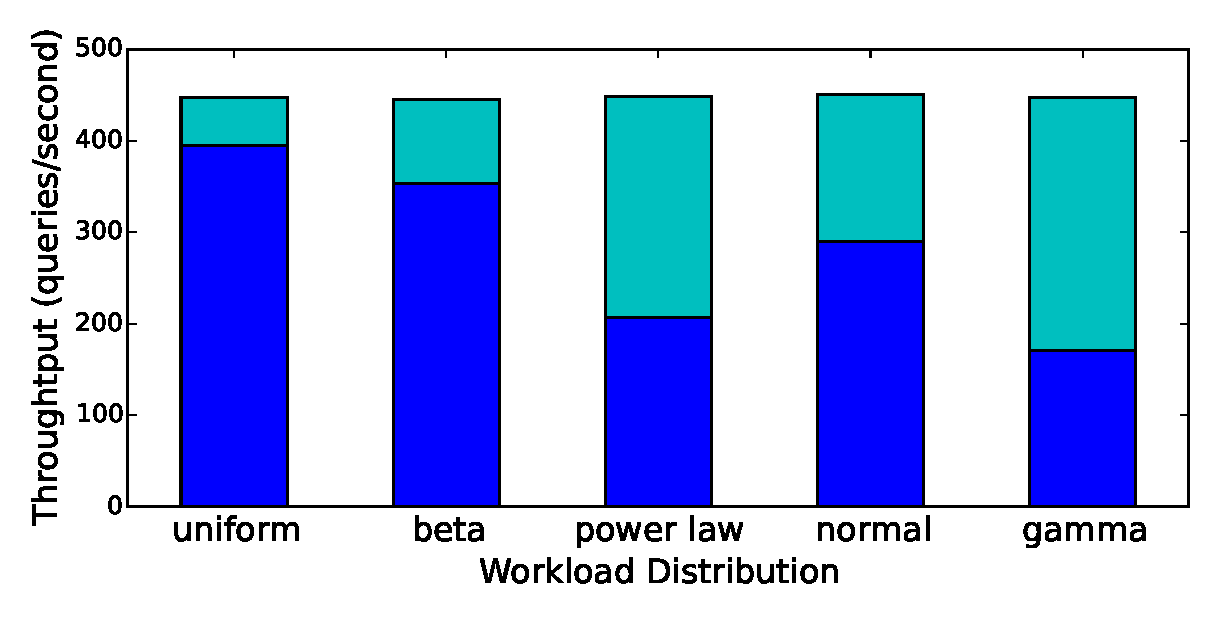
\includegraphics[width=0.8\linewidth]{figures/E34_uniform_suboptimal_tp_stacked_scdm2017.eps}
    \caption{Uniform data placement is suboptimal.
             The lower bar is the measured throughput of uniform placement while
             the upper bar is the performance loss to the idealistic placement.
(Data is a subset of data shown in
\mytable{\ref{tab:throughput_comparison_local}} on Section~\ref{sec:evaluation}.)}
    \label{fig:uniform_suboptimal}
\end{figure}

\myfigure{\ref{fig:uniform_suboptimal}} illustrates the cost of
uniform data replication on non-uniform workloads.
The results for five different workloads are presented on the $x$-axis;
the skew (degree of imbalance) in the workload increases from
left to right.
The \emph{complete} placement solution, where each node has all data,
is an idealistic upper bound on the potential gains of
matching data replication and workload.
% Uniform placement is within 10\% of ideal when the workload is
% uniform.
Because any node can process a request, new requests are sent to the
least loaded node and the performance of \emph{complete} is flat across all
workloads.
In this example, the cluster has twice the minimum capacity, so uniform
replication has two copies of each partition.
Therefore, a request must be sent to
one of the two nodes that hold the data associated
with the request.
Throughput decreases as the
workload skew increases because some nodes are over loaded and
others are under utilized.
While uniform placement achieves 88\% of ideal on uniform workload, it
is only 38\% of ideal on the highly-skewed gamma workload.
This example illustrates the need to properly \emph{replicate} and
\emph{place} data on the nodes of a cluster.


This chapter explores the three dimensions that affect data placement.
The first dimension is \emph{granularity} of data partitions.
Fine-grain (more than one partition per node) placement has costs
(overhead) and benefits (flexibility).
The second dimension is how many \emph{replicas} of each partition.
We let the anticipated demand per partition (\emph{i.e.}, the
\emph{workload}) 
determine the replication factor for each data partition.
The hotter the data, the greater the replication.
The number of data partitions influences how closely the replication
matches the workload.
However,
a coarse-grain partition (one per node) is unlikely to match the
workload.
Last, fine-grain partitioning introduces the
\emph{placement} dimension because there are several ways to distribute
the partitions among the nodes.

We present results from a simulation program that
examines these three dimensions.
We find that coarse-grain placement does not provide sufficient
flexibility to balance non-uniform loads.
A surprisingly small amount of additional partition granularity
is sufficient to load balance and obtain most benefits.
The work presents and evaluates the tradeoff between several
fine-grain placement strategies that either
increase robustness to tolerate workload deviation or
reduce storage footprint.

To further examine these conclusions, our empirical study
on an HPCC cluster\footnote{HPCC Systems is an open source
  \emph{data-analytics computer}---a highly scalable, distributed
  framework for processing and analyzing
  large datasets---supported by LexisNexis Risk Solutions at
  \url{https://hpccsystems.com/}.
}
shows that proper data replication and placement
affect system performance greatly.
The coarse-grain scheme improves system throughput by
$25\%$ and $85\%$ for the normal and power law distribution,
respectively.
A fine-grain placement strategy 
improves query throughput by $52\%$ and $105\%$.
On the most highly-skewed case, the improvement is $166\%$ increase over the
n\"aive solution.

Because data placement relies on a prediction of the upcoming
workload, which will invariably be wrong to some degree.
This chapter, therefore, considers the \emph{robustness}, which
is a measure to describe how sensitive a data placement scheme is to
slightly mis-predicted workloads, of several placement strategies.
Results show that maximizing the number of unique partitions per node
increases the robustness of a placement.
\section{Modeling Data Replication and Placement}
\label{sec:model}

Our work concerns systems in which the dataset
must be partitioned among the nodes because the dataset
is too large to be completely
replicated on each node.
We replicate subsets of the whole dataset in order to increase
throughput and decrease latency.
While replication for availability is critically important, it is not a
subject of this research. 

Distributed, large-scale systems such as
Apache Hadoop, Spark, Cassandra, and Ceph
largely exploit data locality while reducing node-to-node
communication for achieving high horizontal
scaling~\cite{DeanJ2004_MapReduce,zaharia2010spark,Lakshman2010,SageWeil2006Ceph}. 
Data partitions are replicated as the system scales out.
An inefficient data placement scheme is unable to achieve the
optimal system performance and service-level objective (SLO)
violations may occur~\cite{Rodrigues2013,Cruz2013,Trushkowsky2011,Majors2010}.

The goal of this work is to place data partitions onto nodes such
that the performance is maximized for the upcoming workload.
There is a large body of work supporting workload
prediction~\cite{Gmach2007,box2015time,Akdere2012}.
This work assumes that a reliable (though not
necessarily perfect) prediction is provided by some other work.
Instead of solely relying on accurate workload prediction,
systems can dynamically adjust replication factors
and data locations for handling workload changes
~\cite{Lim2010, Trushkowsky2011, Cruz2013}.
This work focuses on determining the optimal
partition granularity, replication factors, and placement strategy.
Our work is complementary to a dynamic approach.

The following model characterizes the 
\emph{data replication and placement problem} in large-scale,
distributed systems. 
Let $M>1$ be the minimum cluster size that is sufficient to hold all
data.
The storage capacity is strictly limited by the amount of data it
physically can store locally.
In many real-world applications, $M$ is in the hundreds of nodes.
However, for this model it is only necessary that $M$ not be equal to
one, which does not require data partitioning.

Let $N$ ($N \ge M$) be the number of nodes in a cluster.
When the workload changes, the cluster expands ($N$ increases)
to meet increased demand and minimize QoS violations, or it contracts
($N$ decreases) to reduce resources and cost. 
But the cluster cannot contract smaller than the $M$ nodes needed to
hold the data.

The data is partitioned into $k \ge 1$ equal-sized data partitions on each node.
Thus, the dataset has $P = Mk$ unique partitions.
Because the cluster has $N$ nodes, there are $S = Nk$ \emph{slots} for
data partitions.
We define the \emph{replication factor}, $R$, as $R=N/M$.
When $R>1$, then $N>M$ and $S > P$ and some partitions will
be replicated among
the ``extra'' slots.
\emph{Coarse-grain} data placement occurs when there is only one
partition per node, $k=1$.
\emph{Fine-grain} data placement, $k>1$, which has more total
data partitions and partition slots, supports more distinct placements
than coarse-grain providing a better opportunity to match the
workload, and increases performance.

\medskip
\begin{tabular}[h]{lll}
  \multicolumn{3}{l}{\textbf{Model parameters}}\\
  ~~~~&\emph{Minimum number of nodes:} & $M>1$\\
  &\emph{Per node granularity:} & $k\ge 1$ \\
  &\emph{Replication factor:} & $R\ge 1$ \\
  \multicolumn{3}{l}{\textbf{Derived terms}}\\
  &\emph{Instantiated nodes:} & $N=RM$\\
  &\emph{Unique data partitions:} & $P = Mk$\\
  &\emph{Slots:} & $S = Nk = RMk$\\
\end{tabular}
\medskip

We present a motivating example below.
The base cluster has four nodes, $M=4$.
The current demand is twice the current capacity.
\myfigure{\ref{fig:dp_before_coarse}}
shows the load per partition on four nodes.
The load is unevenly distributed among the partitions.
In particular, in terms of node capacity the load on the four partitions in
\myfigure{\ref{fig:dp_before_coarse}} is 3.5, 2, 1.5, and 1 (which
conveniently totals 8).
\myfigure{\ref{fig:dp_before_fine}}, shows the same
aggregate demand as it is distributed among 16 partitions, four per
node: $k=4$.
Fine-grain replication gives rise to a \emph{placement} decision.
Redistributing loads helps reduce load imbalance among nodes
by placing highly requested partitions onto least loaded nodes.
In \myfigure{\ref{fig:dp_before_fine_placement}} the load is nearly
balanced: two nodes have a load of 2.125 and two have 1.875.
However, this alone does not help solve the overloading issue
because the workload demand is twice the system capacity.

Suppose the cluster doubles in size to eight nodes exactly meeting
anticipated demand: $R=2$ and $N=8$.
Uniform replication onto eight nodes creates two replicas of each
partition as shown in \myfigure{\ref{fig:dp_uniform}}.
The red box above the two left-most nodes shows the excess demand on those
nodes as 3.5 units of node capacity are serviced by two nodes.
The white regions in the four right-most nodes show the
underutilization because the demand is less than the capacity.

A coarse-grain, non-uniform solution is clearly better
than uniform because \emph{hotter} partitions can be
replicated more than \emph{colder} ones.
For example, in \myfigure{\ref{fig:dp_coarse}} the 3.5 units of P1 are
distributed over three nodes.
Unsurprisingly, a fine-grain solution can better match the demand to
the capacity.
\myfigure{\ref{fig:dp_fine_monochromatic}} shows that demand is perfectly matched to
capacity in this idealized example.


\myfigure{\ref{fig:dp_fine_rainbow}} shows a second placement that also
perfectly balances load but has four unique partitions on each
node.
The nodes in \myfigure{\ref{fig:dp_fine_monochromatic}} have either
one or two unique partitions.
Fewer unique partitions per node reduces the footprint of both primary
(memory) and secondary (disk) storage.
On the other hand,
more unique partitions per node increases the number of nodes that can
respond to a given request, which may better share the load among nodes.

This simple example was constructed to clearly show
the benefits of non-uniform, fine-grain data placement.
Unless the demand is uniformly distributed among the partition (an
extremely unlikely occurrence as explained in
Section~\ref{sec:workloads}) then a n\"aive uniform placement leads to
over- and underutilization.


\begin{figure}[!htbp]
\begin{subfigure}[b]{0.75\textwidth}
    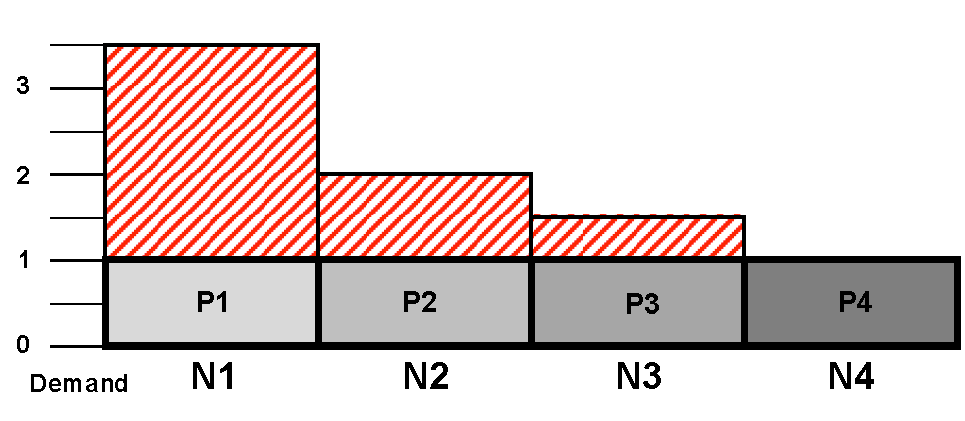
\includegraphics[width=\linewidth]{figures/dp_final_before_coarse.pdf}
    \caption{Coarse-Grain ($M=4,R=1,k=1$)}
    \label{fig:dp_before_coarse}
\end{subfigure}
\begin{subfigure}[b]{0.75\textwidth}
    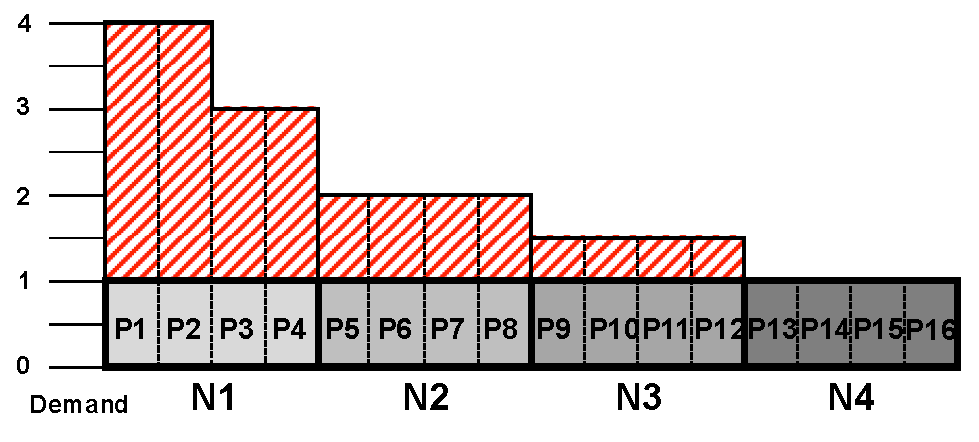
\includegraphics[width=\linewidth]{figures/dp_final_before_fine.pdf}
    \caption{Fine-Grain ($M=4,R=1,k=4$)}
    \label{fig:dp_before_fine}
\end{subfigure}
\begin{subfigure}[b]{0.75\textwidth}
    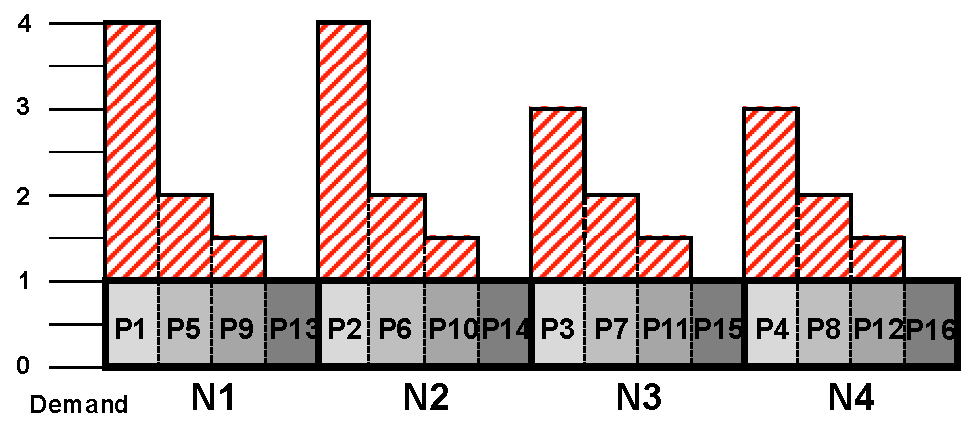
\includegraphics[width=\linewidth]{figures/dp_final_before_fine_R1.pdf}
    \caption{Fine-Grain alternative placement}
    \label{fig:dp_before_fine_placement}
\end{subfigure}
\centering
\caption{The workload demand exceeds the system capacity.}
\label{fig:dp_before}
\end{figure}


\begin{figure}[!htbp]
\begin{subfigure}[b]{0.9\textwidth}
    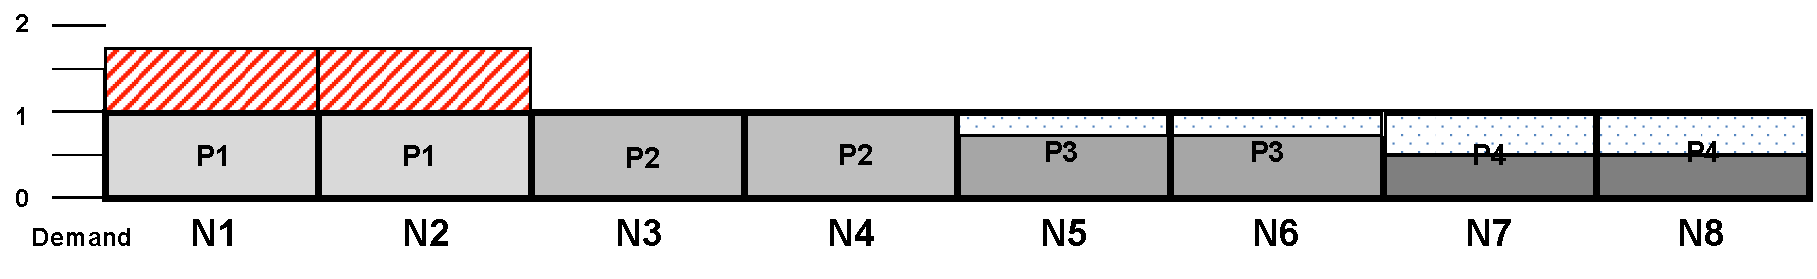
\includegraphics[width=\linewidth]{figures/dp_final_uniform.pdf}
    \caption{Uniform data placement ($M=4,R=2,k=1$)}
    \label{fig:dp_uniform}
\end{subfigure}
\hfill
\begin{subfigure}[b]{0.9\textwidth}
    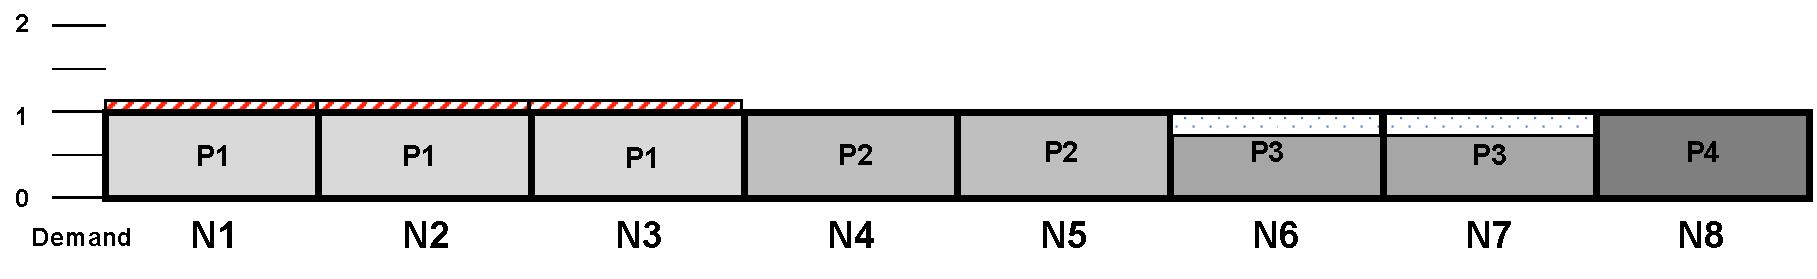
\includegraphics[width=\linewidth]{figures/dp_final_coarse.pdf}
    \caption{Coarse-grain data placement ($M=4,R=2,k=1$)}
    \label{fig:dp_coarse}
\end{subfigure}
\hfill
\begin{subfigure}[b]{0.9\textwidth}
    \includegraphics[width=\linewidth]{figures/dp_final_fine_monochromatic.pdf}
    \caption{Fine-grain \emph{compact} data placement ($M=4,R=2,k=4$)}
    \label{fig:dp_fine_monochromatic}
\end{subfigure}
\hfill
\begin{subfigure}[b]{0.9\textwidth}
    \includegraphics[width=\linewidth]{figures/dp_final_fine_rainbow.pdf}
    \caption{Fine-grain \emph{balanced} data placement ($M=4,R=2,k=4$)}
    \label{fig:dp_fine_rainbow}
\end{subfigure}
\centering
\caption{Different data placement schemes.}
\label{fig:dp_schemes}
\end{figure}

\section{Workloads}
\label{sec:approach}

This section presents the data placement problem.
First, it characterizes the workloads used in the work.
Next, it expounds on the three dimensions of the problem:
(1) granularity, (2) replication, and (3) placement.
Last, it explains and analyzes three data placement methods,
comparing
performance in terms of load imbalance, storage footprint, and robustness.

\subsection{Workload Characteristics}
\label{sec:workloads}

A workload can be described with several critical characteristics,
such as arrival rate and autocorrelation.
Because this work considers data replication and placement, 
the workload characteristic that matters most is access frequency of the
individual elements of the
dataset, such as, the pages of a web server or the keys in an index.
Other characteristics are not factored into
this work because they do not have a direct impact on data replication
or placement.

A uniform workload is atypical and likely artificial,
which is unsurprising because
non-uniform workloads are common in many natural settings
~\cite{Pavlo2012}.
For example, the normal (Gaussian) distribution can be observed
in class score distribution,
while the log-normal distribution is useful to describe
the response file size in web servers~\cite{Barford1998}.
In addition, the power law probability distribution is widely applicable to
web hits, word frequency, personal income, \emph{etc}.\ and tends to
be highly skewed towards a small subset of the full
dataset~\cite{Newman2005}.
That is, a small number of partitions accounts the vast majority of key access
and most of the partitions are touched infrequently. 
Several studies show that frequency of access to different pages or
keys often follows a Zipf or power law distribution.
This has been shown in web servers~\cite{dilley1998web,panteleenko2003web},
video streaming~\cite{sripanidkulchai2004analysis}, 
and Wikipedia traffic~\cite{urdaneta2009wikipedia} to name a few.

In this work, we consider the
\emph{normal} and the \emph{power law} distribution for their
wide appearance in many workloads.
We also consider the \emph{uniform} distribution for a n\"aive baseline,
\emph{beta}, which is less skewed than
\emph{normal} and \emph{power law}, and
\emph{gamma}, which generates the highest skewed workload and
has been used in modeling workloads in storage systems~\cite{Wilkes2001}.


\mytable{\ref{tab:load-imbalance}} shows
the five workload distributions used in the work.
This table presents the distribution of the
requests on each of four partitions ($M=4$, $k=1$).
There are 30,000 unique requests among the 1024 keys,
and the average is 7,500 requests per partition.
The requests-per-node values are ordered in decreasing magnitude.
As expected there are approximately the same number of requests for
each partition in the uniform distribution.
The \emph{max:mean} column shows the ratio of the maximum number of requests
to the average.
Because the total running time is largely dependent on the slowest or
most heavily loaded node, the max-mean ratio foretells the performance
penalty for each workload on a uniform distribution.
The ratio for uniform is 1.01, meaning the maximum is 1\% greater
than the average.
But the highly-skewed gamma distribution has one partition that receives
no requests and one has more than three times the average.
It is clear from \mytable{\ref{tab:load-imbalance}} that in
non-uniform workloads
the maximally loaded partition demands
more resources than the other partitions.
The final column presents access imbalance using the 
\emph{skew} metric~\cite{Pavlo2012}. 

This work evaluates the problem using synthetic workloads.
An alternative is to evaluate using real-world traces.
But such traces are in short supply.
Moreover, a trace represents a very specific situation that may not be
representative of a general class.
Additionally, a trace has many characteristics that are hard to
control.
Using synthetic workloads enables us to evaluate more distributions and
confine the observed effects to the change in distribution.


\begin{figure}[!htbp]
\begin{subfigure}[b]{0.45\textwidth}
    \includegraphics[width=\linewidth]{figures/E45_simulation_imbalance_coarse_std_uniform.eps}
    \caption{uniform}
\end{subfigure}
\begin{subfigure}[b]{0.45\textwidth}
    \includegraphics[width=\linewidth]{figures/E45_simulation_imbalance_coarse_std_beta.eps}
    \caption{beta}
\end{subfigure}
\begin{subfigure}[b]{0.45\textwidth}
    \includegraphics[width=\linewidth]{figures/E45_simulation_imbalance_coarse_std_powerlaw.eps}
    \caption{power law}
\end{subfigure}
\begin{subfigure}[b]{0.45\textwidth}
    \includegraphics[width=\linewidth]{figures/E45_simulation_imbalance_coarse_std_normal.eps}
    \caption{normal}
\end{subfigure}
\begin{subfigure}[b]{0.45\textwidth}
    \includegraphics[width=\linewidth]{figures/E45_simulation_imbalance_coarse_std_gamma.eps}
    \caption{gamma}
\end{subfigure}
\centering
\caption{The load distribution among nodes under the coarse-grain data placement ($M=64, k=1$).}
\label{fig:simulation_imbalance_coarse}
\end{figure}


\begin{figure}[!htbp]
\begin{subfigure}[b]{0.45\textwidth}
    \includegraphics[width=\linewidth]{figures/E45_simulation_imbalance_fine_std_uniform.eps}
    \caption{uniform}
\end{subfigure}
\begin{subfigure}[b]{0.45\textwidth}
    \includegraphics[width=\linewidth]{figures/E45_simulation_imbalance_fine_std_beta.eps}
    \caption{beta}
\end{subfigure}
\begin{subfigure}[b]{0.45\textwidth}
    \includegraphics[width=\linewidth]{figures/E45_simulation_imbalance_fine_std_powerlaw.eps}
    \caption{power law}
\end{subfigure}
\begin{subfigure}[b]{0.45\textwidth}
    \includegraphics[width=\linewidth]{figures/E45_simulation_imbalance_fine_std_normal.eps}
    \caption{normal}
\end{subfigure}
\begin{subfigure}[b]{0.45\textwidth}
    \includegraphics[width=\linewidth]{figures/E45_simulation_imbalance_fine_std_gamma.eps}
    \caption{gamma}
\end{subfigure}
\centering
\caption{The load distribution among nodes under the fine-grain data placement with various $k$ ($M=64, R=2$).}
\label{fig:simulation_imbalance_fine}
\end{figure}


\begin{table}[!htbp]
  \centering
  \caption{Load-imbalance of workloads.}
  \resizebox{\columnwidth}{!}{%
  \begin{tabular}[h]{lrrrrcc}
    \toprule
Distribution & 	\multicolumn{4}{l}{Requests for individual partitions}
    & max:mean & skew\\
\midrule
Uniform & \textbf{7,565} & 7,548 & 7,449 & 7,438 & 1.01 & 0.15\\
Beta & \textbf{10,313} & 10,288 & 4,715 & 4,684 & 1.38 & 0.39\\
Power law & \textbf{17,344} & 8,795 & 3,361 & 500 & 2.31 & 0.60 \\
Normal & \textbf{14,882} & 14,827 & 149 & 142 & 1.98 & 0.74\\
Gamma & \textbf{23,542} & 6,329 & 129 & 0 & 3.14 & 0.77\\
\bottomrule
  \end{tabular}
  }
  \label{tab:load-imbalance}
\end{table}


%%%%%%%%%%%%%%%%%%%%%%%%%%%%%%%%%%%%%%%%
% Approaches
%%%%%%%%%%%%%%%%%%%%%%%%%%%%%%%%%%%%%%%%

\subsection{Data Placement Steps}
\label{sec:dp_methods}

A data placement method requires determining
partition granularity, replication factors, and placement schemes.
Partition granularity represents the smallest unit
for replicating data and calculating loads.
The coarsest granularity is one partition per node ($k=1$), and
the finest is one partition per key.
A small $k$ decreases the likelihood of balancing a non-uniform workload.
However, a large $k$ increases management overhead.

Once the partition granularity $k$ is determined,
the next step
in deriving a solution is determining the number of
replicas for each partition based on the expected workload.
For example, suppose there are four partitions ($P=4$) with a
replication factor of four ($R=4$), then
there are sixteen slots for these partitions ($S=16$) in a
coarse-grain solution.
Given a uniform expected workload the replication factor vector would be 
[4, 4, 4, 4], that is there are four copies of each of the four
partitions. 
For a workload with a normal distribution the replication factor
vector might be [2, 6, 6, 2] and for 
power law it might be [1, 2, 4, 9].
In general, there is no perfect match between the vector and the
anticipated workload.

Assuming that the predicted load on each partition is $\lambda_i$ and the total
load is $\Lambda = \sum_{i=1,P}\lambda_i$.
The replication problem is to determine the \emph{replication vector},
$\vec{R}, R_i \in \mathcal{I}$, such that
$R_i \ge 1~\forall i$  and
$S = \sum_{i=1,P}R_i$.
In words, the replication vector contains the number of replicas (an
integer value) of each partition, such that the total number of
replicas equals the number of slots available.
The replication error is
$E = \sum_{i=1,P} | R_i/S - \lambda_i/\Lambda |$, which is the
accumulation of difference between 
the actual relative
replication of each partition ($R_i/S$) and
the anticipated relative
workload per partition ($\lambda_i/\Lambda$).

%\input{tables/delta_powerlaw}

The last step is assigning the replicas to the slots on the nodes.
For coarse-grain, the number of replicas equals the number of
slots and there is only one possible placement.
But for fine-grain, $k>1$, there are many possible placements.
One placement strategy is to minimize the number of unique
partitions on each node in order to reduce dataset footprint on the
nodes.
We call this strategy \emph{compact}.
If there are multiple choices,
it picks the node with the least load.
The opposite strategy to \emph{compact} is \emph{full},
which maximizes the number of different partitions on each node and
also picks the node with the least load.
The third strategy is placing partitions in order to balance loads as much as possible.
We call this strategy \emph{balanced}. 
We show that although \emph{full} and \emph{balanced} have
different goals, the resultant placements and effects are similar.
Furthermore, \emph{compact} and \emph{full}
balance loads among the
nodes with their best efforts within their given constraints.
Consequently, all three strategies achieve good load balancing, of
course \emph{balanced} is a slightly better at it.
To reiterate:
The goal of \emph{compact} is reducing the number of unique partitions
on each node, which reduces the 
footprint of the data set.
On the other hand, the goal of \emph{full} is to distribute
replicas for the same partition to as many nodes as possible---balancing
the load---with the intent of increasing the availability of hot partitions. 



Our data placement procedure is described in Algorithm \ref{alg:dp}.
This is a framework and therefore, different placement strategies can be used.
The complexity for generating the replication vector is proportional
to the number of partitions, $\mathcal{O}(Mk)$.
Different placement strategies implement distinct
\emph{pick\_node} functions,
which is $\mathcal{O}(N)$.
This function is executed for each slot ($Nk$).
Therefore, the total complexity is of the placement algorithm
is $\mathcal{O}(kN^2)$.
Although it is quadratic, it is in the number of nodes that, even in a
very large cluster, is tractable.
A straightforward Python implementation executes in under few seconds
when $N=256$ and $k=16$.
Furthermore, this solution is a heuristic, it does not find the
optimal solution.
However, the solution is nearly optimal and because it is based on a
prediction of anticipated load optimal is unnecessary.


\begin{algorithm}[!htbp]
 \SetAlgoLined
 \DontPrintSemicolon
 \DontPrintSemicolon
 \KwIn{an historical workload}
 \KwOut{partition placement on each node}
 $M$ := the minimum number of nodes that hold all data\;
 $k$ := the selected partition granularity\;
 $R$ := the replication factor\;
 $loads$ := the predicted loads $\lambda_i$ of partitions\;
 $replicas$ := the replication vector (see Section~\ref{sec:model})

 \For{$p_i$ in $replicas$}{
   \For{$j$=1; $j<=p_i$; $j=j+1$}{
   	 /* strategy is \emph{compact}, \emph{balanced} or \emph{full} */\;
     n := pick\_node(strategy)\;
     assign $p_i$ to $n$
   }
 }
 \caption{Data Placement Procedure}
 \label{alg:dp}
\end{algorithm}




\subsection{Tradeoffs in Placement Strategy}
\label{sec:dp_tradeoff}

Our data placement framework is shown in Algorithm~\ref{alg:dp}.
This framework yields several variants of data placement
when choosing different placement strategies.
This section compares their effects on load balancing and storage footprint.

\subsubsection{Load Balancing}
The primary goal of data placement is distributing workloads evenly among nodes.
A highly skewed system is more likely to encounter performance bottlenecks.
Therefore, a well-balanced system achieves a higher system throughput.
To explore the benefit of fine-grain replication and placement, we
evaluate the effectiveness of 
our data placement schemes in balancing the anticipated workload.
We generated 100 instances of workloads, of 300,000 queries, for each of
the five distributions.
The workload instances vary because the access counts are generated
probabilistically.
Each generated workload is considered a prediction of the upcoming
workload.

First, we evaluate how the replication factor $R$ affects load balancing.
This simulation is conducted with $M=64$ and $k=1$.
We use the box plot, as shown in \myfigure{\ref{fig:simulation_imbalance_coarse}},
to analyze the loads distributed among nodes.
The bottom and top of the rectangle represent the first and third quartile of loads.
The red line is the median, and the red dot is the mean.
To facilitate comparison, the loads are normalized so that the means equal one.
Above the box is the whisker that is calculated by
adding $1.5$ times the interquartile range (IRQ) to the third quartile.
Similarly, the whisker below the box is the first quartile
minus $1.5$ times the IRQ.
The plus signs represent the data points that have the loads
beyond the two whiskers.
These is the standard representation for a box plot.
In a well balanced system, the median and mean values
will be close and the box will be small.

This figure clearly shows that increasing the replication factor
reduces load imbalance to a degree.
However, this alone is insufficient to eliminate
under-utilized loads totally because
increasing the number of replicas only reduces the loads.
The only way to reduce under utilization is
to overlap under and over utilized partitions,
which is not possible in the coarse grain method. 
Therefore, the replication factor alone is not sufficient
for balancing loads because it does not reduce under-utilization.
Take the \emph{gamma} distribution for example,
when $R=1$, most of the nodes are under utilized (low median) and
few nodes have extremely excess loads (large size box).
Doubling the replication factor creates more overloaded nodes
because $R=2$ is not enough to distribute loads.
As $R$ increases, the median value moves closer to the mean and
the variance (the size of box) also decreases,
which suggests over-utilization is mostly addressed.
However, increasing $R$ is still insufficient because
there are still many outliers (beyond the two whiskers).


Next, we examine how much the partition granularity can reduce load imbalance.
We run a set of simulations with $M=64$, $R=2$, and various $k$ values,
and choose \emph{balanced} as the placement scheme.
\myfigure{\ref{fig:simulation_imbalance_fine}} clearly shows that
fine partition granularity greatly reduces load imbalance.
Even in the most skewed workload (gamma), $k=16$ is able to almost perfectly balance loads.
For most workloads, $k=4$ is sufficient to reduce the load imbalance
below $10\%$.
When workloads are highly skewed (the \emph{normal} and \emph{gamma} case),
their load imbalance (the size of box in the figure) drops greatly from $k=1$ to $k=2$
because finer partitioning provides higher flexibility to mix
over- and under-utilized partitions on the same node.
Increasing partition granularity eventually leads to (for all
practical purposes)
perfectly balanced loads.


\begin{figure}[!htbp]
    \centering
    \includegraphics[width=0.8\textwidth]{figures/E42_simulation_colors_resized_powerlaw.eps}
    \caption{The number of unique partitions per node (storage footprint) under different placement schemes.}
    \label{fig:simulation_colors}
\end{figure}

\subsubsection{Storage Footprint}
There are $S=Nk$ choices for placing a partition replica.
When placing multiple replicas of the same partition on the same node,
it reduces the number of unique partitions per node.
When the number of unique partitions per node is lower,
it generally requires lower storage footprint.
A lower storage footprint reduces memory pressure, and may lead to higher cache efficiency.
We run a set of simulations with $M=64$, $R=2$ and various $k$.
This work only presents the results of the \emph{power law} workloads.
Other workload cases show very similar effects.

\myfigure{\ref{fig:simulation_colors}} shows the average number of
unique partitions on each node.
By definition all partitions in 
\emph{full} are unique and it is always 1 (normalized).
\emph{Balanced} is very nearly 1 in all cases.
On the other hand, as $k$ increases, 
\emph{compact} tends to $0.5$, which is $1/R$.
We further investigate how the replication factor affects storage footprint.
\myfigure{\ref{fig:simulation_colors_replication}} shows that the
number of unique partitions tends to $1/R$ as $k$ increases,
which is the desired outcome of the \emph{compact} scheme.


\begin{figure}[!htbp]
    \centering
    \includegraphics[width=0.8\textwidth]{figures/E42_simulation_colors_replication_resized_powerlaw.eps}
    \caption{The number of unique partitions per node under the \emph{compact} method with various $k$.  The number converges at $k=32$, which is equal to $1/R$.}
    \label{fig:simulation_colors_replication}
\end{figure}

\section{Evaluation}
\label{sec:evaluation}

This section presents our evaluation.
We introduce our experimental setup and benchmark
design.
We then evaluate different placement schemes
by measuring query throughput and
testing their robustness to slight workload mispredictions.


\subsection{Experiment Setup}

We conducted our evaluation on Virtual Computing Lab (VCL), a cloud
platform provided by NC State University.
All servers are equipped with 2-core Intel Xeon CPU and 8GB memory
and connected to a 10 Gbit switch. 
VCL only provides limited storage capacity of local disks or
\emph{instance storage}.
This is also the case for many cloud configurations.
In fact, a majority of EC2 instance types in Amazon Web Services (AWS) do not
have any instance storage.
Instead one must mount a remote volume served by a enterprise-level
storage system.
(AWS calls this \emph{elastic block storage}--EBS.)
We evaluate our approach using both instance storage (local disks) and
remote volumes provided by network file system (NFS),
backed by NetApp 2554 filer with dual controllers.

We evaluate our placement schemes on
high performance computing cluster (HPCC)~\cite{middleton2011hpcc}.
HPCC is an open source
data analytics computer developed by LexisNexis Risk
Solutions for processing big data.
They maintain several clusters with more than 100 nodes, the largest
with more than 500, to provide services to their clients.
Experiments were conducted on a HPCC Roxie cluster.
Roxie is a \emph{data delivery engine} that responds to queries.
It finds the answers to requests in an index that is partitioned and,
if desired, replicated across the nodes.
Roxie is optimized to handle massive amounts of concurrent requests
with low latency.

Data replication and placement that fit workload demands
have direct performance impact on performance.
Roxie clusters partition and distribute data
with two replicas per partition by default.
We modified Roxie to incorporate our data placement schemes.
Our approaches are not specific to Roxie.
They should be able to apply to
Apache Hadoop, HBase, Cassandra, and Ceph, providing benefit when
workloads are not uniformly distributed across
keys, partitions or nodes.


\subsection{Workload Generator and Benchmark Suite}

To evaluate the results learned in our simulation, we developed a
distributed benchmark tool 
that is able to issue a large volume of concurrent queries to
Roxie. 
This benchmark tool adopts the master-slave architecture, where
the the master node generates workload according to a workload profile, and
the slave nodes execute the query requests.
This tool is customizable and supports any number of
workload distributions.
This benchmark suite is written in Python, and designed for testing
query performance at large scale.

In our evaluation, we are interested in how placement schemes
with different levels of partition granularity
respond to different types of workload distribution.
We consider \emph{uniform}, \emph{beta}, \emph{power law}, \emph{normal}, and \emph{gamma} distributions.
The beta distribution is defined on the interval $[0, 1]$ with
two shape parameters, $\alpha$ and $\beta$.
We choose $\alpha=2$ and $\beta=2$ for the base case of beta distribution. 
The power law distribution is controlled by the
\emph{shape} parameter and we choose $3$ for the base case.
Regarding the normal (or Gaussian) distribution it has a
\emph{mean} and a \emph{standard deviation} parameter, which is
$0$ and $1$ in our case.
The gamma distribution also has a \emph{shape} parameter and the base case
uses $5$.
%\ick[redundant?] -> we didn't specify the parameters in detail.
A single instance of each workload is used in all the empirical tests
of Roxie so that results can be compared across multiple runs and
different configurations.
The specific workloads used are those shown in
\mytable{\ref{tab:load-imbalance}}.


\subsection{Benchmark Steps}

To best measure the performance, our benchmark service runs
one worker node for each Roxie server, which 
eliminates the performance impact at the client side.
We use separate machines from the Roxie cluster on the VCL for the benchmark service.
The Roxie controller node dispatches requests and synchronizes with workers.
Worker nodes request jobs and execute them as soon as possible.


We generate the five workload distributions
with different access counts to keys.
All datasets are 128GB.
Next, we specify the smallest cluster size $M$,
the replication factor $R$ (which determines
the cluster size $N$), and
the partition granularity $k$.
In our evaluation, $M$ is equal to 4.
The coarse-grain schemes replicate data on
a node basis.
Fine-grain schemes, on the other hand,
divides the data on a node into 32 equal-size partitions
(1GB per partition).

We compare five placement schemes in total.
First, \emph{base} represents the uniform data placement.
It is coarse grain ($k=1$) and not workload aware.
The \emph{coarse} scheme is also coarse-grain but replicates partitions
based on anticipated workload.
For the fine-grain schemes ($k=32$), we consider
\emph{compact} to reduce storage footprint while maximizing cache locality,
and \emph{balanced} to minimize load imbalance among machines.
In our evaluation, we found that the \emph{balanced} and \emph{full} scheme
have comparable performance.
Due to the page limit, we report the results of \emph{balanced} in most cases.
Last, the \emph{complete} is an ``idealistic'' placement where each
node holds the entire dataset.
It represents an upper bound.

\begin{table}[t]
\centering
\caption{Steady-State Throughput Comparison (instance storage)}
\resizebox{\columnwidth}{!}{%
\begin{tabular}{llllll}
\toprule
{} &  Uniform & Beta &  Power Law & Normal  &   Gamma \\
\midrule
\emph{base}          & 394.8            &  353.5            &  206.6             &    290.4             &  171.2 \\
\emph{coarse}        & -                &  367.8 ($4.0\%$)  &  381.9 ($84.9\%$)  &    364.0 ($25.3\%$)  &  309.7 ($80.9\%$) \\
\emph{compact}       & 375.4 ($-4.9\%$) &  377.5 ($6.8\%$)  &  383.2 ($85.5\%$)  &    374.6 ($29.0\%$)  &  374.2 ($118.6\%$) \\
%Rainbow       & 388.6 ($-1.6\%$) &  398.8 ($12.8\%$) &  438.7 ($51.1\%$)  &    416.8 ($101.8\%$) &  438.5 ($156.2\%$) \\
\emph{balanced}      & 408.1 ($3.4\%$)  &  412.6 ($16.7\%$) &  422.8 ($104.7\%$) &    442.5 ($52.4\%$)  &  455.9 ($166.3\%$) \\
%MCMLB         & 447.0 ($6.8\%$) &  449.0 ($14.8\%$) &  484.0 ($56.1\%$)  &    460.0 ($119.4\%$) &  483.0 ($201.9\%$) \\
\emph{complete}      & 446.8 ($13.2\%$) &  445.4 ($26.0\%$) &  448.3 ($117.0\%$) &    450.1 ($55.0\%$)  &  447.0 ($161.1\%$) \\
\bottomrule
\multicolumn{6}{r}{unit: queries/second} 
\end{tabular}
}
\label{tab:throughput_comparison_local}
\end{table}


Our next step is to change the data layout in Roxie to reflect
the desired data placement decision.
The Roxie cluster is restarted to load the new data layout.
To avoid cache interference, the file system cache is cleared
before every benchmark run.

Last, a workload profile is submitted to the benchmark controller.
The controller node generates the query plan accordingly.
In this way, the same stream of requests is presented for each
benchmark, which allows us to verify results with multiple identical
runs and to compare results from different placements.
We collect query throughput during the entire benchmark process.

\subsection{Steady-State Throughput}
\label{sec:throughput}

We conduct this evaluation to test steady-state throughput.
We generate 30,000 requests for each of the five workload
distributions.
We then calculate the average throughput over the sampling period
(the first and last $10\%$ period are not included.)
This measurement ensures we capture the stable throughput, but not
the warm-up period (low throughput) and
the long-tail period (system is not saturated).


\begin{figure}[!htbp]
\begin{subfigure}[b]{0.6\textwidth}
    \includegraphics[width=\linewidth]{figures/E38_robustness_std_beta.eps}
    \caption{Beta}
    \label{fig:robustness_beta}
\end{subfigure}
\begin{subfigure}[b]{0.6\textwidth}
    \includegraphics[width=\linewidth]{figures/E38_robustness_std_powerlaw.eps}
    \caption{Power Law}
    \label{fig:robustness_powerlaw}
\end{subfigure}
\begin{subfigure}[b]{0.6\textwidth}
    \includegraphics[width=\linewidth]{figures/E38_robustness_std_gamma.eps}
    \caption{Gamma}
    \label{fig:robustness_gamma}
\end{subfigure}
    \centering
    \caption{Compare robustness under slight workload mispredictions. The $y$-axis represents queries per second, and starts from 200 for better presentation to tell performance difference.}
    \label{fig:robustness}
\end{figure}


\subsubsection{Local Storage}

Our evaluation starts with storing data required for Roxie queries
on local disks.
This evaluation involves 8 Roxie nodes: $M=4$ and $R=2$.
\mytable{\ref{tab:throughput_comparison_local}} shows the throughput
of proposed replication and placement schemes under
different workloads.
The values in parenthesis are the speedup relative to \emph{base} performance at
the top of each column.
The \emph{base} placement strategy is uniform.
It does not perform well as
the skewness of workload increases.
For example, the power law workload in the uniform data placement
can only achieve $52.3\%$ of the throughput of a uniform workload.
The second strategy is also coarse grain but replicates according to
anticipated workload.
On a uniform workload this is the same as \emph{base}.
It out performs \emph{base} on skewed workloads.
For example, it
achieves $84.9\%$ more throughput than \emph{base} on \emph{power law}.


Two fine-grain approaches, \emph{compact} and \emph{balanced}, which
further improve performance over \emph{coarse}, are also shown.
In the normal workload case, \emph{compact} and \emph{balanced}
improve on \emph{coarse} by an additional $10.6$ and $78.5$ queries per second.
In the gamma case, \emph{balance} adds $146.2$ queries,
a $47.2\%$ improvement over \emph{coarse}.
Workload-aware data placement is preferable for non-uniform workloads.
The fine-grain strategies out perform \emph{coarse} on all the skewed
workloads.
This is attributed to better load balancing.
As skew increases, the benefit from fine-grain increases (because the
load imbalance in \emph{coarse} increases).


\begin{comment}
\begin{table*}[h]
\centering
\caption{Steady-State Throughput Comparison}
\begin{tabular}{llllll}
\toprule
{} &  Uniform & Beta &  Normal &  Power Law &   Gamma \\
\midrule
Base          & 399.0           &  267.0          &  227.0           &    180.0           &  159.0 \\
Coase         & -               &  368.0 ($38\%$) &  362.0 ($59\%$)  &    371.5 ($106\%$) &  309.5 ($\ \ 95\%$) \\
Monochromatic & 402.5 ($0.9\%$) &  409.0 ($53\%$) &  410.0 ($81\%$)  &    403.5 ($124\%$) &  399.0 ($151\%$) \\
Rainbow       & 426.0 ($6.8\%$) &  431.0 ($61\%$) &  405.5 ($79\%$)  &    442.0 ($146\%$) &  427.0 ($169\%$) \\
Complete      & 438.0 ($9.8\%$) &  414.0 ($55\%$) &  433.0 ($91\%$)  &    449.0 ($149\%$) &  431.0 ($171\%$) \\
\bottomrule
\multicolumn{6}{r}{unit: queries/second} 
\end{tabular}
\label{tab:throughput_comparison}
\end{table*}
\end{comment}


\begin{table}[t]
\centering
\caption{Steady-State Throughput Comparison (NFS)}
\resizebox{\columnwidth}{!}{%
\begin{tabular}{llllll}
\toprule
{} &  Uniform & Beta &  Power Law &  Normal &   Gamma \\
\midrule
\emph{base}       & 446.1            &  383.1            &  220.2             &    393.3             &  176.4 \\
\emph{coarse}     & -                &  396.4 ($3.5\%$)  &  415.3 ($88.6\%$)  &    379.6 ($29.4\%$)  &  327.9 ($85.9\%$) \\
\emph{compact}    & 403.7 ($-9.5\%$) &  416.2 ($8.7\%$)  &  401.3 ($82.3\%$)  &    407.1 ($38.8\%$)  &  407.8 ($131.1\%$) \\
%Rainbow   & 447.3 ($0.3\%$)  &  428.1 ($11.8\%$) &  474.0 ($61.6\%$)  &    469.0 ($113.0\%$) &  481.5 ($172.9\%$) \\
\emph{balanced}   & 447.6 ($0.3\%$)  &  440.8 ($15.1\%$) &  454.0 ($106.2\%$) &    469.7 ($60.1\%$)  &  485.9 ($175.5\%$) \\
%MCMLB     & 447.9 ($0.4\%$)  &  448.8 ($17.2\%$) &  479.8 ($63.6\%$)  &    455.5 ($106.9\%$) &  482.0 ($173.2\%$) \\
\emph{complete}   & 484.2 ($9.0\%$)  &  485.6 ($26.8\%$) &  492.4 ($123.7\%$) &    495.0 ($68.8\%$)  &  490.0 ($177.8\%$) \\
\bottomrule
\multicolumn{6}{r}{unit: queries/second} 
\end{tabular}
}
\label{tab:throughput_comparison_nfs}
\end{table}


The \emph{complete} solution out performs all others, including both fine-grain
solutions.
This is because while the workload was probabilistically generated
over 30,000 requests.
The workload for each small window of requests does not always reflect
the overall workload.
In such cases, \emph{complete} performs better.
However, \emph{complete} is generally not feasible
when dataset is too large to fit into one node.

Overall, workload-aware data placement significantly increases query throughput.
Using fine partition granularity better balances the load.
\emph{Balanced} performs better than \emph{compact}, indicating that
the benefit of a smaller footprint is less than the cost of poorer load
balancing.
The \emph{balanced} scheme is occasionally competitive with \emph{complete}.

\subsubsection{Remote Storage}
Next, we evaluate our proposed schemes against data storing on remote storage.
The Roxie cluster size and the number of benchmark clients remain the same
with the local storage case.
\mytable{\ref{tab:throughput_comparison_nfs}} details the throughput numbers.
This evaluation confirms the general observations seen in the instance
storage test.
However, the throughput is higher using remote storage.
While somewhat counter intuitive, it is not unheard.
This occurs because local storage uses plain commodity disks and the
% not sure the original sentence is grammerly correct
filer uses high-performance disks as well as aggressive caching.
Moreover, the I/O demand does not exceed the capacity of the NFS server.
Therefore, the additional network traffic is not creating a
performance bottleneck.


\subsection{Robustness Comparison}
\label{sec:robustness}

We are interested in how sensitive a placement scheme is to minor
deviations in the anticipated workload.
(Tables~\ref{tab:throughput_comparison_local} and
\ref{tab:throughput_comparison_nfs} show performance degradation for
major deviations.)
We say a placement scheme is more \emph{robust} when the scheme works
well even when the actual workload is slightly different from the
anticipated workload.
We pick different parameters for generating slight workload variance.
For example, we change the shape parameter in the power law distribution.
Therefore, it becomes either less or more skewed.
We create two less and two more skewed workloads for each type.

\myfigure{\ref{fig:robustness}} shows how different placement schemes react
to workload shifts.
The figure shows the average throughput and the standard deviation
 of the placement schemes under the four ``shifted'' workloads
The figure indicates that the coarse-grain scheme
under performs in both average (lower) and deviation (greater)
compared to the fine-grain schemes.

The \emph{compact} scheme is better than \emph{coarse} but its performance is not as
good as the \emph{balanced} scheme.
The \emph{balanced} scheme overall exhibits higher throughput than
\emph{coarse} and \emph{compact}.
More importantly, \emph{balanced} shows consistent standard deviation
in three workloads.
The highest performance degradations in each workload are
$2\%$, $6\%$ and $3\%$
while the \emph{compact} scheme shows
$3\%$, $5\%$ and $14\%$ (increasing as skewness increases) degradation respectively.
% The \emph{balanced} shows $6\%$ performance loss at most.
% balanced
%  - beta: 436.41 vs 444.75
%  - power law: 442.22 vs. 471.82
%  - gamma: 472.98 vs. 487.88
% compact
%  - beta: 396.85 vs. 410.53
%  - power: 388.71 vs. 408.26
%  - gamma: 350.19 vs. 408.02
The above suggests than \emph{balanced} is more robust then
\emph{compact}, which is robust than \emph{coarse}.
There is little difference between \emph{balanced} and \emph{full} in either
average throughput or standard deviation.
This is because there is little difference in the placement of
partitions---that is, the balanced scheme tends to have a high degree of
unique partitions on each node.



\subsection{Micro Benchmark}

We have presented the steady-state throughput in Section~\ref{sec:throughput}.
In this section, we further examine why different placement schemes
lead to large performance difference.

We investigate resource utilization of different placement schemes
for understanding the tradeoff between the \emph{compact} and
\emph{balanced} scheme. 
We collect system statistics
(\textit{dstat}~\cite{dstat} and \textit{cachestat}~\cite{cachestat})
during the entire benchmark runs.
\mytable{\ref{tab:micro_nfs}} presents the system statistics, and
metrics are normalized to the smallest value in each metric group,
except the \emph{max:mean} ratio. 
This normalization better shows the difference between placement schemes.
Except \emph{mean \%CPU}, a system is more efficient when
the metrics listed are small.
These metrics are collected from the benchmark runs under the gamma workload.
Other workloads present very similar trends.

First, we examine CPU utilization across all Roxie nodes.
The average CPU utilization indicates whether Roxie is fully saturated,
and the \emph{max:mean} metric tells whether loads are well balanced
among Roxie nodes.
In the \emph{base} scheme, CPU utilization is the lowest and load imbalance
is the highest, which explains why uniform data placement under performs.
Workload-aware replication eliminates load imbalance while
improving CPU utilization.
Fine-grain partition further reduces load imbalance,
as in the \emph{balanced} scheme.

\begin{table}[ht]
\centering
\caption{Normalized System Statistics of Roxie Servers}
\resizebox{\columnwidth}{!}{%
\begin{tabular}{lllllll}
\toprule
	& Metrics	&	\emph{base}	&	\emph{coarse} & \emph{compact} & \emph{balanced} & \emph{complete} \\
\midrule
\multirow{2}{*}{Load Balancing} & \% CPU (mean)		& \textbf{1.00} (13\%) & 2.29   & 2.37 & 3.11 & 2.97     \\
		                        & \% CPU (max:mean) & 2.01 & 1.34   & 1.23 & 1.1    & 1.14     \\
\midrule
\multirow{3}{*}{Cache Locality} & cache misses (sum)     & 1.13 & 1.24   & \textbf{1.00} (659K) & 1.26 & 1.22     \\
		                        & dirty pages (sum)     & 1.20 & 1.47   & \textbf{1.00} (200K) & 1.52 & 1.29     \\
		                        & cache sizes (max) & 2.11 & 1.51   & \textbf{1.00} (825MB)   & 1.17 & 1.15     \\
\midrule
\multirow{2}{*}{Efficiency}     & I/O wait (mean) & 1.39 & 6.73   & \textbf{1.00} (2.35\%) & 2.48 & 2.55     \\
		                        & TCP connections (mean)   & 2.40 & 1.53   & 1.31 & 1.10 & \textbf{1.00} (1357) \\
%		                        & disk read         & 2.72 & 2.00   & 1.09 & \textbf{1.00} & 3.48    \\
\bottomrule
\end{tabular}
}
\label{tab:micro_nfs}
\end{table}



Second, we examine the benefits of packing multiple replicas into the same node,
as in the \emph{compact} scheme.
\mytable{\ref{tab:micro_nfs}} shows that cache misses and dirty pages
are significantly lower in the \emph{compact} scheme.
Besides, \emph{compact} has much lower cache sizes, $17\%$ lower than
\emph{balanced} and $51\%$ less than the \emph{coarse} scheme.
Although the \emph{compact} scheme outperforms others in cache locality and
requires less cache,
it does not generate the highest query throughput.
A possible explanation is that requests do not greatly benefit from better cache locality.
We suspect the \emph{compact} scheme is useful especially when query applications
require costly read operations.
% We will need to further investigate this case.

Third, we compare I/O wait time and the number of TCP connections
for comparing their efficiency.
A lower I/O wait time indicates that systems do not waste much time on slow I/O operations.
The \emph{compact} scheme, with maximum cache locality, has the lowest I/O wait value.
The number of TCP connections at a given time is related to processing efficiency.
We observe that the \emph{balanced} scheme yields a lower number of TCP connections
than the other schemes, suggesting that requests complete more quickly.


\subsection{Summary}
Our evaluation provides empirical data to support our findings
in the simulation.
First, workload-aware data placement, both the coarse and fine grain methods,
reduces load imbalance, thereby improving system throughput.
However, the coarse-grain approach is insufficient
when workload is highly skewed.
Finer partitioning further balances the loads and in many cases,
the \emph{balanced} scheme has comparable performance to \emph{complete}
(an ``idealistic'' placement).
Furthermore, both \emph{balanced} and \emph{full} are robust while
\emph{compact} reduces storage footprint to $1/R$. 



%% 
\section{Related Work}
\label{sec:related}

The data replication and placement issues have been extensively studied
in several research domains
including memory cache~\cite{Leff1993,Zaman2011},
distibuted storage systems~\cite{Lim2010},
NoSQL database~\cite{Rodrigues2013,Cruz2013,Corbett2013}
traditional retaional databases~\cite{Pavlo2012,Curino2010},
content delivery network (CDN)~\cite{Laoutaris2006}, etc.

Data replication is a common technique to increase
system performance and availability.
Many distributed systems use multiple replicas to
increase reliability and availability as well as improve system
performance~\cite{hbase,SageWeil2006Ceph}.
This chapter focuses on data replication and
its impact on system performance.
Data placement, on the other hand, determines the locations of data.
Apache Hadoop, for example, writes a replica locally and
two replicas in another rack to improve
system performance~\cite{Xie2010,Eltabakh2011}.
Our work makes contributions in three ways.
First, partition granularity determines the basic unit to calculate load.
Second, data replication is governed by anticipated workload.
Last, data placement chooses the slots on servers for maximizing
load balancing or exploiting cache locality.

Ceph is a distributed storage system
that supports configurable replication factors
for the placement group~\cite{SageWeil2006Ceph}.
Similarily, Apache Hadoop~\cite{hadoop} accepts separate replication factors
for different data chunks.
Optimizing the number of replications per object or data chunk
is a challenging task.
AptStore proposes the Popularity Prediction Algorithm (PPA) by
analyzing file system logs and adjusts replication factors accordingly
for files on Apache Hadoop~\cite{Krish2013}.
Scarlett combines offline log analysis and online prediction to
accurately estimate block popularity~\cite{Ananthanarayanan2011}.
Results show that replicating hotter data avoids bottlenecks,
thereby improving the performance of MapReduce jobs.
% These works greatly improve distributed storage performance but
% do not totally answer all the essential properties of
% data replication and placement.

The NoSQL database is a popular repository for large-scale data
because of they support extreme horizontal
scaling~\cite{Lakshman2010,Chang2008,hbase,mongodb}.
%\cmt{add more citations, eg, hbase, reddis,dynamodb, mongodb.}
Studies have shown that non-uniform query key
causes performance issues.
AUTOPLACER \cite{Rodrigues2013} optimizes the placement
for the top-k objects in the distributed key-value store.
To minimize the maintenance cost of large number of objects,
AUTOPLACER proposes the probabilistic data structure (PAA)
to reduce routing latency.
MET \cite{Cruz2013} is an elasticity framework that 
optimizes data placement to fit workload characteristics for HBase.
It is able to reconfigure HBase dynamically when an HBase cluster
requires expansion or contraction.
MET found that heterogeneous machines can easily lead to load imbalance.
To balance the load on each server, MET groups data partitions
according to their access pattern.
MET models the cost of placing data partitions on nodes, and
uses Longest Processing Time (LPT) to minimize the cost,
which maximizing load sharing among nodes.
%\cmt{what is makespan?}
The above implements a system that replicates and places data according to
data access pattern.
Our work explores how data replication and placement schemes
affect system performance under different workload distribution.

%%%%%%%%%%%%%%%%%%%%%%%%%%%%%%%%%%%%%%%%%%%%%%%%%%%%%%%
% moved fig this from model.tex to make it float to first page of mode
%%%%%%%%%%%%%%%%%%%%%%

%%%%%%%%%%%%%%%%%%%%%%%%%%%%%%%%%%%%%%%%%%%%%%%%%%%%%%%

Elastic storage dynamically expands or contracts a storage cluster.
The elastic controller is responsible for
provisioning resources and adjusting data replication and placement
for efficient storage configurations.
The SCADS director \cite{Trushkowsky2011} is an elastic controller
that automatically scales out a storage system to meet stringent
performance requirements. 
SCADS adopts a model-based approach to correlate request workload and
latency. 
It keeps track of the hottest bins (groups of data), and
dynamically moves these bins to different servers for balancing the load.
SCADS also creates performance models to predict workload and server capacity
for better estimating query latency.
Lim et al. propose a design of elastic storage\cite{Lim2010}.
Scaling a storage system poses challenges such as actuator delays,
measurement accuracy and interference with applications.
Their work puts emphasis on the elastic controller, whereas
we discover the relationship between
workload characteristics and data placement
when scaling a data-intensive application.

Sharding is a common technique to distribute load by
partitioning data across distributed server nodes.
More specifically, sharding is an approach that partitions data
according to keys, where partitions are placed
on different servers independently~\cite{Cattell2011}.
This horizontal scaling enables a distributed system to scale efficiently.
NoSQL databases, such as BigTable~\cite{Chang2008}, HBase~\cite{hbase}
and Cassandra~\cite{Lakshman2010}, rely on sharding
to efficiently balance load.

For relational databases, sharding is heavily used to support
a large volume of queries.
Schism uses graph-partitioning algorithms
to determine the optimal partitioning
for minimizing the cost of distributed transactions~\cite{Curino2010}.
The proposed fine-grained data partition minimizes
the required number of distributed transactions for database applications.
Pavlo \emph{et al}. develop a database tool that is able to generate
optimal database designs for parallel OLTP systems~\cite{Pavlo2012}.
They propose a new search algorithm for partitioning database and
create a cost model to minimize the coordination cost
while maximizing load balance.
Spanner is a semirelational database that
manages replicated data globally and performs resharding
at runtime for better load balancing~\cite{Corbett2013}.
Slicer is an auto-sharding service designed by Google~\cite{Adya2016}.
To leverage Slicer, users are required to
associate incoming requests with a key.
Slicer dynamically maps the key to a proper task
for maximizing load balance.
The above studies implement either
a sharding mechanism or design s generic sharding service,
while our work focuses on understanding the tradeoff
between different data placement schemes
when data partitions required proper placement to
meet workload distribution.

\section{Conclusion}
\label{sec:conclusion}

Efficient deployment of large-scale, distributed systems with
an irregular workload requires both cluster sizing and data placement.
We show the uniform distribution is (unsurprisingly) poor for
typical, non-uniform workloads.
This work further shows that coarse-grain replication can reduce
over-utilization but is unable to address under-utilization.
Finer partition granularity reduces both under- and
over-utilization.
With fine-grain partitioning there is a placement decision.
Maximizing the number of unique partitions per node increases robustness
to workload misprediction,
while minimizing the number reduces storage
footprint.
Our empirical study using an HPCC Roxie cluster shows
the benefit of footprint reduction does not offset cost due to poorer
load balancing.
However, we do not believe this is universally true.

This work focuses on the dimension and tradeoffs of various data
replication and placement strategies.
For our future work, we plan to implement an elastic controller
that incorporates our proposed data placement schemes.
In an elastic system, the gains of the optimal placement must be
offset by the cost of data movement.
Calculating this data movement cost remains as a future work.

\chapter{Conclusions and Future Work}
\label{chapter:conclusion}

\section{Thesis Revisited}
Modern software systems come with a lot of configuration options, which can be tweaked to modify the functional or
non-functional (e.g., throughput or runtime) requirements. Finding
the good or optimal configuration to run a particular workload is essential
since there is a significant difference between the best and the
worst configurations. Many researchers report that modern software
systems come with a daunting number of configuration options~\cite{xu2015hey}.
The size of the configuration space increases exponentially with the
number of configuration options. The long runtimes or cost required
to run benchmarks make this problem more challenging.

Prior work in this area used a machine learning method
to model the configuration space accurately. The model is built sequentially,
where new configurations are sampled randomly, and the
quality or accuracy of the model is measured using a holdout set. This strategy
makes these methods unsuitable in a practical setting since they can be very expensive. On the other hand, there are software systems for which an accurate model cannot be
built.

In this thesis, we introduced techniques and method, which can find good configurations while minimizing the search cost. The central insight of this thesis is: to build a machine learning model (not accurate) which
can differentiate between the good and not so good solutions. 

The important lessons, we learned during the preparation of the thesis are:
\begin{itemize}
    \item \textbf{Clustering: } Early attempts managed to use random sampling along with machine learning models to build accurate models, which can then be used to find good configurations. However, random sampling and accurate machine learning models can lead to an expensive model building process. We attempt to \textbf{reduce the cost of the model building by adding the idea of stratified sampling instead of random sampling} i.e.; we try to cluster the configuration space using a top-down clustering and sampling from each sub-population. We have found stratified sampling can significantly reduce the cost of model building and also reduce the variance in the model built. \\
    \noindent\textbf{Lessons Learned: } Even though we found the stratified sampling approach of \what works for the software systems explored in our paper~\cite{nair2017faster}. However, while performing external validation (with a more diverse set of software systems), we found that \what is not efficient (as shown by our preliminary study). Upon further investigation, we found that we make an important assumption: ``our clustering algorithm (WHERE in our case) returns meaningful cluster''. This assumption meant that we know the distance function applicable to the configuration space, i.e., configurations with shorter distance is similar to the configurations with a larger distance. The ineffectiveness of \what is primarily because our assumption did not hold for the newer configuration spaces.
    
    \item \textbf{Ranking: } A retrospective look on the prior work including our work, made us realize that researchers have been tackling the problem of finding good configuration by transforming the problem to a building accurate model problem. However, the fundamental idea in this work is to use ranking as an approach for building models. The ranking is a useful paradigm to solve the software configuration optimization because (1) ranking is the ultimate goal, (2) Ranking is extremely robust since it is only mildly affected by errors or outliers, and (3) Ranking reduces the number of training samples required to train a model.\\
    \noindent\textbf{Lessons Learned:} The model is built sequentially, where new configurations are sampled randomly, and the quality or accuracy of the model is measured using a holdout set. The size of the holdout set in some cases could be up to 20\% of the configuration space and need to be evaluated (i.e., measured) before even the machine learning model is entirely built. This strategy makes these methods unsuitable in a practical setting since the generated holdout set can be (very) expensive. 
    
    \item \textbf{Sequential Model-based Optimization:}  The problem of finding the (near) optimal configuration is expensive and often infeasible using the current techniques. A useful strategy could be to build a machine learning model which can differentiate between the good and not so good solutions. \flash, a Sequential Model-based Optimization (SMBO), is a useful strategy to find extremes of an unknown objective. \flash is efficient because of its ability to incorporate prior belief as already measured solutions (or configurations), to help direct further sampling. Here, the prior represents the already known areas of the search (or performance optimization) problem. The prior can be used to estimate the rest of the points (or unevaluated configurations). Once one (or many) points are evaluated based on the prior, the posterior can be defined. The posterior captures the updated belief in the objective function. This step is performed by using a machine learning model, also called \textit{surrogate model}. The concept of \flash can be simply stated as:
    \begin{itemize}
        \item Given what one knows about the problem,
        \item what can be done next?
    \end{itemize}
    The ``given what one knows about the problem'' part is achieved by using a machine learning model whereas ``what can be done next'' is performed by an acquisition function. Such acquisition function automatically adjusts the exploration (``should we sample in uncertain parts of the search space'') and exploitation (``should we stick to what is already known'') behavior of the method.\\
    \noindent\textbf{Lessons Learned: } Much current research (including all the approaches discussed in this thesis) has explored this problem, usually by creating performance models that predict performance characteristics. While this approach is cheaper and more effective than manual configuration, it still incurs the expensive of extensive data collection about the software. This is undesirable since this data collection has to be repeated if ever the software is updated on the workload of the system changes abruptly. In such a scenario, all prior research suffers from the same drawback: these approaches do not learn from previous optimization experiments and must be rerun whenever the environment of the experiments change. Note our use of the term environment. This refers to the external factors influencing the performance of the system such as workload, hardware, version of the software.
    
\end{itemize}


\section{Future Work}
There are many fruitful avenues of research that are worthwhile to pursue but
beyond the scope of this dissertation. Here are just a few directions: 

\noindent\textbf{Can expert knowledge be used to increase the rate of convergence?}\\
During our many conversations with the people in the industry, we get pushback regarding the automated approaches. The common theme of this conversation is generally, ``we have been configuring our software systems for decades, and we have people who can configure these systems in their sleep''. While this line of reasoning is generally flawed and there are several pieces of evidence (as discussed in our related work session). Pooyan Jamshidi has shown several such examples. Figure~\ref{fig:expert_wrong} is one such example with Cassandra.
\begin{figure}[t]
\centering
\includegraphics[width=\columnwidth]{Chapter-Conclusion/Figures/ExpertWrong.png}
\caption[Comparison between default configurations,  configurations selected by experts and optimal configuration.]{Comparison between default configurations,  configurations selected by experts and optimal configuration. From \url{http://tiny.cc/existingTechniques}.
}
\label{fig:expert_wrong}
\end{figure}
However, the rate of convergence is \flash is dependent on the initial configurations (currently selected using random sampling). So, if expert knowledge can be successfully extracted and embedded into the initial sample, it can further reduce the cost of optimization. There has been some effort made in this direction~\cite{feurer2018scalable, Hsu2018Scout}.

\noindent\textbf{Can we learn from our experience to increase the rate of convergence or decrease the cost?}\\
Transfer learning can only be useful in cases where the source environment is similar to the target environment. If the source and the target are not similar, knowledge should not be transferred. In such an extreme situation, transfer learning can be unsuccessful and can lead to a \textit{negative transfer}. Prior work on transfer learning focused on ``What to transfer'' and ``How to transfer'', by implicitly assuming that the source and target are related to each other. Hence, that work failed to address “When to transfer.” Jamshidi et al.~\cite{jamshidi2017transfer} alluded to this and explained when transfer learning
works but, did not provide a method which can help in selecting a
suitable source. There is a need for some effort in solving the problem of performance optimization by choosing an appropriate source to transfer knowledge. We have made some progress in this area~\cite{nair2018transfer}.

\noindent\textbf{Does learning about landscape~\footnote{Landscape refers to features of the problem such as modality (local optimal and plateau), basins of attractions~\cite{mersmann2011exploratory}} provide us with information about which search strategy to use?}\\
The techniques used in \flash (model and the acquisition function) is a subset of a larger space of options. During the development phase of \flash, we tried various options and narrowed down on the existing options using trial and error. However, there may be configuration spaces where \flash is not effective. Since the configuration space is currently a black box to us, there is a need for a fast technique to sample and understand that \textbf{landspace} quickly. This information can then be used to select the right combination of model and acquisition function. This problem is currently explored as a different problem namely algorithm configuration, and there is some progress in this area~\cite{mersmann2011exploratory}. There is also a great tool available to get a head start in this domain~\cite{hanster2017flaccogui}.

\noindent\textbf{Can these ideas be applied to other domains?}\\
In an abstract sense, the problems discussed in this thesis falls under a broad realm of black-box optimization. The only challenging component (or rather a constraint) to this problem is each evaluation is costly. Hence, we need to be aware of the cost (both time and computing resources). There are various other domains where the methods, discussed in this thesis, can be applied such as hyperparameter tuning, cloud configuration, etc. We made some progress in applying these techniques in the cloud configuration~\cite{Hsu2018Arrow, Hsu2018Micky, Hsu2018Scout}. 

\noindent\textbf{How to optimize for a large macro-system which involves many micro-systems?}
The software systems, explored in this thesis, are standalone system and not a collection of heterogeneous systems. We hypothesize that in such collective systems the configuration of one of the participating software system can affect the performance of another participating software system. In such cases, how can we alter the techniques discussed in this thesis to be valuable in such situations. 

\section{Epilogue}
The prior works in the area of performance optimization have transformed the problem of finding good configurations into a modeling problem. Researchers have tried to solve this problem by building accurate models, which made this process of optimization (using models) expensive. In this thesis, we have shown that the problem of performance optimization can be tacked as an optimization problem and not a modeling problem. This can be done by building inaccurate models and use the models to explore new regions of the configuration space. 

The idea of this thesis can be best encapsulated as: 
\begin{center}
\begin{flushleft}
    \hspace{1.5cm}\textbf{``There's no sense in being precise when you }\\
    \hspace{1.5cm}\textbf{don't even know what you're talking about.''}\\
    \hspace{1.5cm}\hfill\textbf{--- John von Neumann}\\
\end{flushleft}
\end{center}

% 5. It is always difficult to know which configurations are truly valid? So, given specific examples of valid configuration can build a model which could potentially tell us which configurations could be valid or not? Some form of a classification model?
% 7. Given that the performance of a particular system running a specific benchmark is highly variable (because of its environment, for example, variability in cloud xxxbubbleup) how can we build models which can tolerate multiple levels of fidelity?
\restoregeometry


%%---------------------------------------------------------------------------%%
%%  Bibliography 

%%  You can use the bibitem list.
%\bibliographystyle{unsrt}
%\begin{%thebibliography}{99}
%\bibitem{cb02}
%Casella, G. and Berger, R.L. (2002)
%\newblock {\it Statistical Inference, Second Edition.}
%Duxbury Press, Belmont, CA.
%
%\bibitem{t06}
%Tsiatis, A.A. (2006)
%\newblock {\it Semiparametric Theory and Missing Data.}
%Springer, New York.
%
%\end{thebibliography}

%% or use BibTeX
%\bibliography{Ortiz-thesis}{}
%\bibliographystyle{plain}
%\nociterec{*}

%\bibliographystyle{plain}
%\bibliography{thesis}{}
%\nociterec{*}

%\bibliographystyle{plainnat}%plainnat is necessary to enable the use of citet. Natbib style file.
%\bibliography{Ortiz-thesis2}
%\ensureoddstart
\begin{spacing}{1}
 \setlength\bibitemsep{11pt} %22pt = 2*11pt, where fontsize is 11pt
 \phantomsection
 \addcontentsline{toc}{chapter}{{\uppercase{\bibname}}} %\textorpdfstring and \uppercase needed due to hyperref package http://www.latex-community.org/forum/viewtopic.php?f=44&t=16601
 %\vspace{-0.5in}
\titleformat{\chapter}[display]{\bf\filcenter
}{\chaptertitlename\ \thechapter}{11pt}{\bf\filcenter}
%\titlespacing*{\chapter}{0pt}{-0.5in-9pt}{22pt}
\titlespacing*{\chapter}{0pt}{0.0in-9pt}{22pt}

\printbibliography[heading=myheading]
\end{spacing}
%\bibliographystyle{apalike}


%%---------------------------------------------------------------------------%%
% Appendices
%\ensureoddstart
%\restoregeometry
%\appendix
%\newgeometry{margin=1in,lmargin=1.25in,footskip=\chapterfootskip, includehead, includefoot}


%\chapter{Appendix}

TBD.

% \section{A First Section}
% \section{A Second Section}


%\restoregeometry

%%---------------------------------------------------------------------------%%
%\ensureoddstart
\backmatter


\end{document}
